%==============================================================================
%==============================================================================
\documentclass[12pt]{report}
\usepackage{epsf}
\usepackage{graphicx}
\usepackage{include/harvard}
\usepackage{alltt}
\usepackage{longtable}
\usepackage{moreverb}
\usepackage{amsmath,amssymb}
\usepackage{url}
\usepackage{subfigure}
\pagestyle{plain}
\topmargin=0pt
\textwidth=6.75in
\textheight=9in
\evensidemargin=-15pt
\oddsidemargin=-15pt
%==============================================================================
\newcommand{\autoversion}{0.9.6}

\newcommand{\ds}{\displaystyle}
\newcommand{\beq}{\begin{equation}} 
\newcommand{\eeq}{\end{equation}}
\def\norm#1{\parallel#1\parallel}
\def\abs#1{\mid#1\mid}
\def\eps{\epsilon}
\def\R{{\rm R}}
\def\Rn{{\rm R}^n}

\newcommand{\AUTO}{{\cal AUTO}~}
\newcommand{\AUTOc}{\AUTO 2000~}
\newcommand{\AUTOold}{\AUTO 97~}
\newcommand{\AUTOolder}{\AUTO 94~}

\newcommand{\python}{{\cal Python}}

\newcommand{\emp}{\emph}

% A font for AUTO parameters
%\newcommand{\parf}[1]{\filef{#1}}
\newcommand{\parf}[1]{{\tt #1}}

% A font for UNIX commands
%\newcommand{\commandf}[1]{{\it #1}}
\newcommand{\commandf}[1]{{\tt #1}}

% A font for environment variables
%\newcommand{\envf}[1]{\filef{#1}}
\newcommand{\envf}[1]{{\it #1}}

% A font for function names
%\newcommand{\funcf}[1]{\filef{#1}}
\newcommand{\funcf}[1]{{\bf #1}}

% A font for filenames
%\newcommand{\filef}[1]{{\tt #1}}
\newcommand{\filef}[1]{{\sf #1}}

% A font for ftp sites and web pages
%\newcommand{\webf}[1]{\commandf{#1}}
\newcommand{\webf}[1]{{\sl #1}}

%==============================================================================
\def\norm#1{\parallel#1\parallel}
\def\abs#1{\mid#1\mid}
\def\eps{\epsilon}
\def\R{{\rm R}}
\def\Rn{{\rm R}^n}
%==============================================================================
%==============================================================================
\begin{document}
\bibliographystyle{include/agsm} 
%
\title{
\LARGE {\cal AUTO}-07P :\\ 
\Large CONTINUATION AND BIFURCATION SOFTWARE \\
\Large FOR ORDINARY DIFFERENTIAL EQUATIONS\\ 
\author{
\Large Eusebius J. Doedel\\
\Large Concordia University\\
\Large Montreal, Canada\\
\\
with major contributions by\\
\\
Alan R. Champneys (Bristol),
Thomas Fairgrieve (Toronto),
\\
Yuri Kuznetsov (Utrecht),
Bart Oldeman,
Randy Paffenroth (Pasadena),
\\
Bj\"orn Sandstede (Surrey),
Xianjun Wang,
and
Chenghai Zhang.\\
}}
\date{August 2007}
\maketitle
\tableofcontents
%
%
\newpage
~
\vskip.50truein
\subsection*{Preface}
This is a guide to the software package {\cal AUTO}
for continuation and bifurcation problems in ordinary differential 
equations.
Earlier versions of {\cal AUTO} were described in 
\citename{Do:81} \citeyear{Do:81},
\citename{DoKe:86} \citeyear{DoKe:86},
\citename{DoWa:95a} \citeyear{DoWa:95a},
\citename{WaDo:95b} \citeyear{WaDo:95b},
\citename{AUTO:97} \citeyear{AUTO:97},
\citename{AUTO:2000} \citeyear{AUTO:2000},
For a description of the basic algorithms see
\citename{DoKeKe:91a} \citeyear{DoKeKe:91a},
\citename{DoKeKe:91b} \citeyear{DoKeKe:91b}.
{\cal AUTO} incorporates the {\cal HomCont} algorithms of
\citename{ChKu:94} \citeyear{ChKu:94},
\citename{ChKuSa:95} \citeyear{ChKuSa:95}
for the bifurcation analysis of homoclinic orbits.
The Floquet multiplier algorithms were written by
\citename{Fa:94} \citeyear{Fa:94},
\citename{FaJe:91} \citeyear{FaJe:91}.
A GUI was written by
\citename{XJW:94} \citeyear{XJW:94}.
The Python CLUI is the work of Randy Paffenroth.

\vskip1.00truein
\subsection*{Acknowledgments}
The first author is much indebted to H.~B.~Keller 
of the California Institute of Technology for his inspiration,
encouragement and support.
He is also thankful to {\cal AUTO} users and research collaborators who have 
directly or indirectly contributed to its development,
in particular, 
Jean Pierre Kern\'evez, UTC, Compi\`egne, France;
Don Aronson, University of Minnesota, Minneapolis; and 
Hans Othmer, University of Utah.
Some material in this document related to the computation of connecting orbits
was developed with Mark Friedman, University of Alabama, Huntsville.
Also acknowledged is the work of Nguyen Thanh Long,
Concordia University, Montreal, on the graphics program {\cal PLAUT}.
Special thanks are due to Sheila Shull, California Institute of Technology,
for her cheerful assistance in the distribution of {\cal AUTO} over a long period
of time.
Over the years, the development of {\cal AUTO} has been supported by
various agencies through the California Institute of Technology, and
by research grants from NSERC (Canada).

The development of {\cal HomCont} has benefitted from help and advice from, 
among others, 
W.-J. Beyn, Universit\"{a}t Bielefeld,
M.~J. Friedman, University of Alabama,
A. Rucklidge, University of Cambridge, 
M. Koper, University of Utrecht,
C.~J. Budd, University of Bath,
Fabio Dercole, Politecnico di Milano, and
Frank Schilder, University of Surrey,
Financial support for this collaboration was also received from the U.K.
Engineering and Physical Science Research Council and the Nuffield Foundation.

\newpage
~
\subsection*{License}
{\cal AUTO} is available under the terms of the BSD license:\\
\begin{footnotesize}
~\\
Copyright \copyright~1979--2007, E.~J.~Doedel, California Institute of
Technology, and Concordia University.  All rights reserved.\\
~\\
Redistribution and use in source and binary forms, with or without
modification, are permitted provided that the following conditions are
met:
\begin{itemize}
\item Redistributions of source code must retain the above copyright
  notice, this list of conditions and the following disclaimer. 
  
\item Redistributions in binary form must reproduce the above copyright
  notice, this list of conditions and the following disclaimer listed
  in this license in the documentation and/or other materials
  provided with the distribution.
  
\item Neither the name of the copyright holders nor the names of its
  contributors may be used to endorse or promote products derived from
  this software without specific prior written permission.
\end{itemize}
THIS SOFTWARE IS PROVIDED BY THE COPYRIGHT HOLDERS AND CONTRIBUTORS
"AS IS" AND ANY EXPRESS OR IMPLIED WARRANTIES, INCLUDING, BUT NOT  
LIMITED TO, THE IMPLIED WARRANTIES OF MERCHANTABILITY AND FITNESS FOR
A PARTICULAR PURPOSE ARE DISCLAIMED. IN NO EVENT SHALL THE COPYRIGHT 
OWNER OR CONTRIBUTORS BE LIABLE FOR ANY DIRECT, INDIRECT, INCIDENTAL,
SPECIAL, EXEMPLARY, OR CONSEQUENTIAL DAMAGES (INCLUDING, BUT NOT
LIMITED TO, PROCUREMENT OF SUBSTITUTE GOODS OR SERVICES; LOSS OF USE,
DATA, OR PROFITS; OR BUSINESS INTERRUPTION) HOWEVER CAUSED AND ON ANY
THEORY OF LIABILITY, WHETHER IN CONTRACT, STRICT LIABILITY, OR TORT  
(INCLUDING NEGLIGENCE OR OTHERWISE) ARISING IN ANY WAY OUT OF THE USE
OF THIS SOFTWARE, EVEN IF ADVISED OF THE POSSIBILITY OF SUCH DAMAGE. 
\end{footnotesize}

%==============================================================================
%==============================================================================
\chapter{Installing {\cal AUTO}.} \label{ch:Installing_AUTO}
%==============================================================================
%==============================================================================
\section{ Installation.} \label{sec:Installation}
%The {\cal AUTO} files {\filef auto.ps.gz, auto.tar.gz} and {\filef README} 
%are available via FTP from 
%directory {\filef pub/doedel/auto} at \url{ftp.cs.concordia.ca}.
The {\cal AUTO} file \filef{auto07p-0.4.tar.gz} is
available via \url{http://indy.cs.concordia.ca/auto}.
%The {\filef README} file contains the instructions for printing this manual.
Below it is assumed that you are using the Unix (e.g. \emph{bash}) shell 
and that the file \filef{auto07p-0.4.tar.gz} is in your main directory.

While in your main directory, enter the commands
\commandf{gunzip auto07p-0.4.tar.gz},
followed by \commandf{tar xvfo auto07p-0.4.tar}.
This will result in a directory \filef{auto}, 
with one subdirectory, \filef{auto/07p}. 
Type \commandf{cd auto/07p}
to change directory to \filef{auto/07p}.
Then type
\commandf{./configure}~,
to check your system for required compilers and libraries.
Once the \filef{configure} script has finished you 
may then type \commandf{make} to compile \AUTO
and its ancillary software.
The \filef{configure} script is designed to detect the details
of your system which \AUTO requires to compile successfully.
If either the \filef{configure} script or the \filef{make} command
should fail, you may assist the \filef{configure} script by giving
it various command line options.  Please type \commandf{./configure --help}
for more details.
Upon compilation, you may type 
\commandf{make clean}  
to remove unnecessary files.

To run \AUTO you need to set your environment variables correctly.
Assuming \AUTO is installed in your home directory, the following
commands set your environment variables so that you will be able to
run the \AUTO commands, and may be placed into your \filef{.login},
\filef{.profile}, or \filef{.cshrc} file, as appropriate.  If you are
using a \commandf{sh} compatible shell, such as \commandf{sh},
\commandf{bash}, \commandf{ksh}, or \commandf{ash} enter the command
\commandf{ source~ {\rm \$}HOME/auto/07p/cmds/auto.env.sh}.  On the
other hand, if you are using a \commandf{csh} compatible shell, such
as \commandf{csh} or \commandf{tcsh}, enter the command \commandf{
source~ {\rm \$}HOME/auto/07p/cmds/auto.env}.

The Graphical User Interface (GUI) requires the {\cal X-Window} system
and {\cal Motif} or {\cal LessTif}.
Note that the GUI is not strictly necessary, since {\cal AUTO} can be
run very effectively using the Unix Command Language User Interface (CLUI).
Moreover, long or complicated sequences of {\cal AUTO} calculations can
be programmed using the alternative Python CLUI. 
THe GUI is not compiled by default. To compile
\AUTO with the GUI, type \commandf{./configure --enable-gui}
and then \commandf{make} in the directory \filef{auto/07p}.

The new graphic tool for \AUTO data visualization, PLAUT04, is
compiled by default, but depends on a few libraries that may not be
in a standard installation of a typical Unix-like
system. These libraries may be available as optional packages,
though. The packages Coin3D (version 2.2 or higher), SoQt
(1.1.0 or higher), and simage (1.6 or higher) are recommended.
Many Linux distributions provide packages for some or all
these libraries, using names such as Coin2-Devel, SoQt-Devel (Fedora)
and libcoin40-dev, libsoqt-dev, and libsimage-dev (Debian and Ubuntu).
For Mac OS X there exist Fink packages.
The libraries can also be downloaded from
\url{http://www.coin3d.org/download/} and compiled from source.

Instead of SoQt it is possible to use the SoXt library, which
interfaces with (Open)Motif or LessTif (version 2.0 or higher)
instead of Qt. The user interface has a few problems with LessTif
though, in particular it is likely to crash on 64-bit machines, so the
Qt version or (Open)Motif is recommended.

As a third alternative, one can download SGI's implementation of the
Open Inventor libraries from:
\url{ftp://oss.sgi.com/projects/inventor/download/}
Because SGI's implementation for Linux cannot show text correctly, 
we recommend that Coin is used instead of SGI's implementation. 

If you need to compile and install one of the libraries
from the source code available at the above web site, and you
find that, after that, PLAUT04 still does not work then you might need to
adjust the environment variable {\tt LD\_LIBRARY\_PATH} to include
the location of these libraries, for instance {\tt /usr/local/lib}.

The \filef{configure} script checks
for these libraries and outputs a warning if any of these libraries
cannot be found. It first checks for SoQt, and then for SoXt, unless
you pass {\tt --disable-plaut04-qt} as an option to \filef{configure}.
If the libraries are not available you can still compile
all other components of \AUTO using \filef{make}.

For timing purposes, the file \filef{auto/07p/src/autlib1.f}
contains references to the function {\it etime}.
Similarly, this file contains references to the
subroutine {\it FLUSH} to avoid buffering of screen output when
running \AUTO from Python. These routines are not part of any
Fortran standard but are common extensions. The \filef{configure}
script checks if your compiler supplies them. If they are not
supplied then the dummy replacement routines in \filef{src/compat.f}
are used.

The PostScript conversion command \commandf{@ps} is compiled by
default. Alternatively you can type \commandf{make} in the directory
\filef{auto/07p/tek2ps}.
To generate the on-line manual, type \commandf{make} in \filef{auto/07p/doc}.

To prepare {\cal AUTO} for transfer to another machine,
type \commandf{make superclean}
in the directory \filef{auto/07p} before creating the \filef{tar}-file. 
This will remove all executable, object, and other non-essential files, and
thereby reduce the size of the package.

Some {\cal EISPACK} routines used by {\cal AUTO} for computing eigenvalues and
Floquet multipliers are included in the package
(\citename{EISPACK:76} \citeyear{EISPACK:76}).

\subsection{Installation on Mac OS X}
\AUTO runs on Mac OS X using the above instructions provided that
you have the development tools
installed. You do not need to start an X server to run AUTO. To be able
to plot in the Python CLUI, \AUTO uses \filef{pythonw} instead of
\filef{python}. This should happen automatically.

The old plotting tool {\cal PLAUT} may not display fonts. To solve
this issue you would need to obtain a different version of xterm; see
\url{http://iparrizar.mnstate.edu/~juan/urania/2007/07/19/xterm-tektronix-emulation-broken-on-macos}
or 
\url{http://sourceforge.net/project/showfiles.php?group_id=21781}.
Apple is aware of this problem.

\subsection{Installation on Windows}
A native, light-weight solution for running AUTO on Windows is
to use GFortran, MSYS (see \url{http://www.mingw.org}),
combined with a native Win32 version of Python,
obtained at \url{http://www.python.org}. To install this setup:
\begin{itemize}
\item
Install Python from \url{http://www.python.org}.
\item
Install the minimal Unix-like environment MSYS from
\url{http://www.mingw.org}. You do not need to install MinGW
itself.
\item
Install GFortran from \url{http://gcc.gnu.org/wiki/GFortran}.
\item
Open a CMD.EXE window (click Start, Run, type {\tt cmd}
in the input box and press the Enter key), and run {\tt sh} in the
MSYS directory, for instance, using
\filef{ c:\textbackslash msys\textbackslash 1.0\textbackslash
bin\textbackslash sh $--$login $-$i }
(the Python CLUI does not work in the default MSYS shell environment
 accessed by its desktop icon).
\item
The {\tt sh} command put you in a home directory, where you can unpack
\AUTO using \filef{gunzip} and \filef{tar}, as described above.
\item
Make sure that the {\tt gfortran} and {\tt python} binaries
are in your {\tt PATH}, and that their directories are at the front of it.
You can do this, for instance, using the shell command
\commandf{export PATH="/c/Python24:/c/Program Files/gfortran/bin:\$PATH" }.
You can also inspect, edit and then source the file
\filef{auto/07p/cmds/auto.env.sh} to achieve this.
\item
Now you should be able to run configure, make, and run \AUTO as
shown above.
\end{itemize}

Alternatively, \AUTO runs on Windows as above using the Unix-like
environment Cygwin (see \url{http://www.cygwin.com}). You should have
at least the default installation, \filef{gcc}, \filef{gfortran},
\filef{make}, and \filef{python} installed. The 2D-plot command
is not as reponsive in Cygwin Python as in the above native setup, however.

In both cases, an X server is not necessary, unless you wish to try to run
PLAUT or the GUI. With some effort it may be possible to use PLAUT04
on Windows (without an X server) using Coin, SoQt, and Qt.

\section{ Restrictions on Problem Size.} \label{sec:Restrictions}
There are size restrictions in the file {\tt auto/07p/include/auto.h}
on the following {\cal AUTO}-constants~:
the effective number of equation parameters {\tt NPAR}, and
the number of stored branch points {\tt NBIF} for algebraic problems,
See Chapter~\ref{ch:AUTO_constants} 
for the significance these constants. 
Their maxima are denoted by the  corresponding constant followed by an{\tt X}.
For example, {\tt NPARX} in {\tt auto.h} denotes the maximum value 
of {\tt NPAR}.
If any of these maxima is exceeded in an {\cal AUTO}-run then a message 
will be printed.
The exception is the the maximum value of {\tt NPAR},
which, if exceeded, may lead to unreported errors.
Upon installation {\tt NPARX}=36; it should never be decreased below that value;
see also Section~\ref{sec:Restrictions_on_PAR}.
Size restrictions can be changed by editing {\tt auto.h}.
This must be followed by recompilation by typing {\it make} 
in directory {\tt auto/07p/src}.

Note that in certain cases the {\it effective dimension} may be greater
than the user dimension.
For example, for the continuation of folds,
the effective dimension is 2{\tt NDIM}+1 for algebraic equations,
and 2{\tt NDIM} for ordinary differential equations, respectively.
Similarly, for the continuation of Hopf bifurcations,
the effective dimension is 3{\tt NDIM}+2.
 
 
\section{Compatibility with Earlier Versions.} \label{sec:Compatibility}
Unlike earlier versions, \AUTO can no longer be compiled using a pure
Fortran 77 compiler, but you need at least a Fortran 90 compiler.
A free Fortran 95 compiler, GFortran, is shipped with most recent
Linux distributions, or can be obtained at
\url{http://gcc.gnu.org/wiki/GFortran}, which contains binaries for
Linux, Mac OS X and Windows. \AUTO was also tested with the free
compiler {\tt g95}, and there exist various, untested, commercial Fortran
9x compilers as well.

The {\cal AUTO} input files are now called 
{\tt c.xxx} (the constants file),
and
{\tt h.xxx} (the {\cal HomCont} constants file, only used with {\cal HomCont});
the output files are called
{\tt b.xxx} (the bifurcation-diagram-file),
{\tt s.xxx} (the solution-file),
and
{\tt d.xxx} (the diagnostics-file).
There are also minor changes in the formatting of these files 
compared to recent versions of {\cal AUTO}, such as {\cal AUTO97} 
and {\cal AUTO2000}.
The main change compared to {\cal AUTO97} is that there is now a
programmable Python CLUI.

When upgrading from {\cal AUTO2000}, you can continue to use
equations-files written in C. However, there is now a strict
difference between indexing of the array {\tt par[]} in the
C file and the references to it using {\tt PAR()} in constants
files and output, using {\tt par[i]=PAR(I+1)}. In practise this
means that you do not have to change the C file, but need to
add 1 to all parameter indices in the constant files, namely
{\tt ICP(I)}, {\tt THL(I)}, and {\tt UZR(I)}. For example,
the period is referenced by {\tt par[10]} in the C file,
but by {\tt PAR(11)} in the constants file. Equation files
written in C are used in the homoclinic branch switching
demo in Chapter~\ref{ch:HomCont_hbs}.
 
\section{Parallel Version.} \label{sec:Parallel}
\AUTO contains code which allows
it to run in on parallel computers.  Namely,
it can use either OpenMP to run most of its code in parallel
on shared-memory multi-processors, or the MPI message passing
library.
When the \filef{ configure} script is run it will try to
detect if the Fortran compiler supports OpenMP; examples
are Gfortran 4.2 and the Intel Fortran Compiler.
If it is successful the necessary compiler flags are used
to enable OpenMP in \AUTO.
To force the \filef{ configure} script not to use OpenMP,
one may type \commandf{ ./configure --without-openmp},
and then type \commandf{ make}.
On the other hand, unless there is some
particular difficulty, we recommend that that the 
\filef{ configure} script be used without arguments, since the
parallel version of \AUTO may easily be controlled,
and even run in a serial mode,  
through the use of the environment variable {\tt OMP\_NUM\_THREADS}.

For example, to run the \AUTO executable \filef{ auto.exe}
in serial mode you just type \commandf{ export OMP\_NUM\_THREADS=1}.
To run the same command in parallel on 4 processors you type 
\commandf{export OMP\_NUM\_THREADS=4}. Without any {\tt OMP\_NUM\_THREADS}
set the number of processors that \AUTO will use can be equal to the
actual number of processors on the system, or can be equal to one;
this is system-dependent.

The MPI message passing library is not used by default. You can enable it
by typing  \commandf{ ./configure --with-mpi }. If OpenMP and MPI are
both used then \AUTO uses mixed mode, with MPI parallelisation
occurring at the top level.

Running the MPI version is somewhat more complex because of the fact
that MPI normally uses some external program for starting the
computational processes.  The exact name and command line options of
this external program depends on your MPI installation.  A common name
for this MPI external program is \filef{ mpirun}, and a common command
line option which defines the number of computational processes is \filef{
-np}.  Accordingly, if you wanted to run the MPI version of \AUTO
on four processors, with the above external program, you would
type \filef{ mpirun -np 4 file.exe}.  Please see your local MPI
documentation for more detail.

%==============================================================================
%==============================================================================
\chapter{ Overview of Capabilities.} \label{ch:Overview}
%==============================================================================
%==============================================================================
\section{ Summary.} \label{sec:Summary}
{\cal AUTO} can do a limited bifurcation analysis of algebraic systems
\begin{equation} \label{1} 
  f( u , p ) = 0 ,  \qquad  f(\cdot,\cdot) , u \in \Rn.
\end{equation}
The main algorithms in {\cal AUTO}, however, are aimed at the continuation
of solutions of systems of ordinary differential equation (ODEs) of the form
\begin{equation} \label{2} 
 u'(t) = f\bigl( u(t) , p \bigr) , 
  \qquad  f(\cdot,\cdot) , u(\cdot) \in \Rn,
\end{equation}
subject to boundary (including initial) conditions and integral constraints.
Above, $p$ denotes one or more free parameters,

These boundary value algorithms also allow {\cal AUTO} to do certain stationary 
solution and wave calculations for the partial differential equation (PDE)
\begin{equation} \label{3} 
  u_t = D u_{xx} + f( u , p ), 
  \qquad  f(\cdot,\cdot) , u(\cdot) \in \Rn,
\end{equation}
where $D$ denotes a diagonal matrix of diffusion constants.

The basic algorithms used in {\cal AUTO},
as well as related algorithms, can be found in 
\citename{HBK:77} \citeyear{HBK:77},
\citename{HBK:86} \citeyear{HBK:86},
\citename{DoKeKe:91a} \citeyear{DoKeKe:91a},
\citename{DoKeKe:91b} \citeyear{DoKeKe:91b}.

Below, the basic capabilities of {\cal AUTO} are specified in more detail.
Some representative demos are also indicated.
 
\section{ Algebraic Systems.} \label{sec:algebraic_systems}
Specifically, for (\ref{1}) {\cal AUTO} can~:~
 
\begin{itemize}
\item[-]
  Compute solution families.\\  (Demo {\tt ab}; Run~1.) 
\item[-]
  Locate branch points, continue these in two parameters,
  and automatically compute
  bifurcating families. \\ (Demos {\tt pp2}; Run~1 and {\tt apnf}.)
\item[-]
  Locate Hopf bifurcation points and continue these in two
  parameters. \\ (Demo {\tt ab}; Runs~1 and 5.)
\item[-]
  Locate folds (limit points) and continue these 
  in two parameters. \\(Demo {\tt ab}; Runs~1,3,4.)
\item[-]
  Do each of the above for fixed points
  of the discrete dynamical system 
  $u^{(k+1)}= f( u^{(k)}, p )$ \\ (Demo {\tt dd2}.)
\item[-]
  Find extrema of an objective function along solution families
  and successively continue such extrema in more parameters.
  \\ (Demo {\tt opt}.)
\end{itemize}


\section{ Ordinary Differential Equations.} \label{sec:ODEs}
For the ODE (\ref{2}) the program can~:~
 
\begin{itemize}
\item[-]
  Compute families of stable and unstable periodic
  solutions and
  compute the Floquet multipliers, that determine stability, along
  these families.
  Starting data for the computation of periodic orbits are
  generated automatically at Hopf bifurcation points. \\
  (Demo {\tt ab}; Run~2.)
\item[-]
  Locate folds, branch points, period doubling bifurcations,
  and bifurcations to tori, along families of periodic solutions. 
  Branch switching is possible at branch points and at period 
  doubling bifurcations.  \\
  (Demos {\tt tor}, {\tt lor}.)
\item[-]  Continue folds and period-doubling bifurcations, 
  in two parameters. \\ (Demos {\tt plp}, {\tt pp3}.)
  The continuation of orbits of fixed period is also
  possible. This is the simplest way to compute curves of
  homoclinic orbits, if the period is sufficiently large.
  \\ (Demo {\tt pp2}.)
\item[-]  Do each of the above for {\it rotations}, i.e., when some of the
  solution components are periodic modulo a phase gain of a
  multiple of $2 \pi$. \\
  (Demo {\tt pen}.)
\item[-]  Follow curves of homoclinic orbits and detect and continue
  various codimension-2 bifurcations, using the {\cal HomCont} algorithms of 
  \citename{ChKu:94} \citeyear{ChKu:94},
  \citename{ChKuSa:95} \citeyear{ChKuSa:95}.\\
  (Demos  {\tt san}, {\tt mnt}, {\tt kpr}, {\tt cir},
  {\tt she}, {\tt rev}.)
\item[-]  Locate extrema of an integral objective functional along a family 
  of periodic solutions and successively continue such extrema 
  in more parameters. \\
  (Demo {\tt ops}.)
\item[-]
  Compute curves of solutions to (\ref{2}) on $[0,1]$, subject to general
  nonlinear boundary and integral conditions.
  The boundary conditions need not be separated, i.e., they may
  involve both $u(0)$ and $u(1)$ simultaneously.
  The side conditions may also depend on parameters.
  The number of boundary conditions plus the number of integral
  conditions need not equal the dimension of the ODE, 
  provided there is a corresponding number of additional
  parameter variables. \\
  (Demos {\tt exp}, {\tt int}.)
\item[-]
  Determine folds and branch points along
  solution families to the above boundary value problem.
  Branch switching is possible at branch points.
  Curves of folds can be computed in two parameters.\\
  (Demos {\tt bvp}, {\tt int}.)
\end{itemize}
 


\section{ Parabolic PDEs.} \label{sec:Parabolic_PDEs}
For (\ref{3}) the program can~:~
 
\begin{itemize}
\item[-]
  Trace out families of spatially homogeneous solutions.
  This amounts to a bifurcation analysis of the algebraic
  system (\ref{1}). However, {\cal AUTO} uses a related system instead,
  in order to enable the detection of bifurcations to wave train
  solutions of given wave speed. More precisely, bifurcations
  to wave trains are detected as Hopf bifurcations along fixed
  point families of the related ODE
  \begin{equation} \label{4} \begin{array}{cl}
  & u'(z) = v(z) ,\\
  & v'(z) =-D^{-1}  \bigl[ c~v(z) + f\bigl( u(z) , p \bigr) \bigr], \\
  \end{array} \end{equation}
  where $z = x - ct$ , with the wave speed $c$ specified by the user.\\
  (Demo {\tt wav}; Run~2.) 
\item[-]
  Trace out families of periodic wave solutions to (\ref{3}) that emanate
  from a Hopf bifurcation point of Equation~\ref{4}.
  The wave speed $c$ is  fixed along such a family, but
  the wave length $L$, i.e., the period of periodic solutions 
  to (\ref{4}),
  will normally vary. If the wave length $L$ becomes large,
  i.e., if a homoclinic orbit of Equation~\ref{4} is approached,
  then the wave tends to a solitary wave solution of (\ref{3}). \\
  (Demo {\tt wav}; Run~3.) 
\item[-]
  Trace out families of waves of fixed wave length $L$ in two parameters. 
  The wave speed $c$ may be chosen as one of these parameters.
  If $L$ is large then such a continuation gives a family
  of approximate solitary wave solutions to (\ref{3}).\\
  (Demo {\tt wav}; Run~4.) 
\item[-]
  Do time evolution calculations for (\ref{3}), given periodic
  initial data on the interval $[0,L]$.
  The initial data must be specified on $[0,1]$ and
  $L$ must be set separately because of internal scaling.
  The initial data may be given analytically or
  obtained from a previous computation of wave trains, solitary
  waves, or from a previous evolution calculation.
  Conversely, if an evolution calculation results in a
  stationary wave then this wave can be used as starting data
  for a wave continuation calculation.\\
  (Demo {\tt wav}; Run~5.)
\item[-]
  Do time evolution calculations for (\ref{3}) subject to user-specified
  boundary conditions.
  As above, the initial data must be specified on $[0,1]$ and the space
  interval length $L$ must be specified separately.
  Time evolution computations of (\ref{3}) are adaptive in space and
  in time. Discretization in time is not very accurate~: only
  implicit Euler. Indeed, time integration of (\ref{3}) has only been
  included as a convenience and it is not very efficient.
  (Demos {\tt pd1}, {\tt pd2}.)
\item[-]
  Compute curves of stationary solutions to (\ref{3}) subject to user-specified
  boundary conditions.
  The initial data may be given analytically, obtained from a previous 
  stationary solution computation, or from a time evolution calculation.\\
  (Demos {\tt pd1}, {\tt pd2}.)
\end{itemize}
 
In connection with periodic waves,
note that (\ref{4}) is just a special case of (\ref{2}) and
that its fixed point analysis is a special case of (\ref{1}).
One advantage of the built-in capacity of {\cal AUTO} to deal with
problem (\ref{3}) is that the user need only specify $f$, $D$, and $c$.
Another advantage is the compatibility of output data for
restart purposes. This allows switching back and forth between
evolution calculations and wave computations.

\section{ Discretization.} \label{sec:Discretization}
  {\cal AUTO} discretizes ODE boundary value problems
  (which includes periodic solutions) by the method of orthogonal 
  collocation using piecewise polynomials with 2-7 collocation points 
  per mesh interval (\citename{dBSw:73} \citeyear{dBSw:73}).
  The mesh automatically adapts to the solution to equidistribute
  the local discretization error (\citename{RuCr:78} \citeyear{RuCr:78}).
  The number of mesh intervals and the number of collocation points
  remain constant during any given run, although they may be changed 
  at restart points.
  The implementation is {\cal AUTO}-specific. In particular, the choice of
  local polynomial basis
  and the algorithm for solving the linearized collocation systems
  were specifically designed for use in numerical bifurcation analysis.
  
%==============================================================================
%==============================================================================
\chapter{ User-Supplied Files.} \label{ch:User_supplied_files}
%==============================================================================
%==============================================================================
The user must prepare the two files described below.
This can be done with the GUI described in Chapter~\ref{ch:GUI}, 
or independently.

\section{ The Equations-File {\tt xxx.f90}, or {\tt xxx.f}, or {\tt xxx.c}} 
A source file {\tt xxx.f90} containing the Fortran routines
{\tt FUNC}, {\tt STPNT}, {\tt BCND}, {\tt ICND}, {\tt FOPT}, and {\tt PVLS}.
Here {\tt xxx} stands for a user-selected name. 
If any of these routines is irrelevant 
to the problem then its body need not be completed.
Examples are in {\tt auto/07p/demos}, where, e.g.,
the file {\tt ab/ab.f} defines a two-dimensional dynamical system,
and the file {\tt exp/exp.f} defines a boundary value problem.
The simplest way to create a new equations-file is to copy 
an appropriate demo file.
For a fully documented equations-file see
{\tt auto/07p/demos/cusp/cusp.f90} or {\tt auto/07p/gui/aut.f}.
In GUI mode, this file can be directly loaded with the GUI-button 
{\it Equations/New}; see Section~\ref{sec:GUI_Menu_bar}.
 
The equations-file can either be written in fixed-form (old-style)
Fortran (.f), free-form Fortran (.f90) or in C (.c).

\section{ The Constants-File {\tt c.xxx}} 
{\cal AUTO}-constants for {\tt xxx.\{f,f90,c\}} are normally expected 
in a corresponding file {\tt c.xxx}.
Specific examples include {\tt ab/c.ab}
and {\tt exp/c.exp} in {\tt auto/07p/demos}.
See Chapter~\ref{ch:AUTO_constants}
for the significance of each constant.

\newpage
\section{ User-Supplied Routines.} \label{sec: User_supplied_routines}
The purpose of each of the user-supplied routines in
the file {\tt xxx.{f90,f}} is described below.
  
\begin{itemize}
\item[-] {\tt FUNC}~:~
  defines the function $f(u,p)$ in (\ref{1}), (\ref{2}), or (\ref{3}).
\item[-] {\tt STPNT}~:~
  This routine is called only if {\tt IRS}=0 
(see Section~\ref{sec:IRS} for {\tt IRS}),
  which typically is the case for the first run.
  It defines a starting solution $(u,p)$ of (\ref{1}) or (\ref{2}).
  The starting solution should not be a branch point.\\ 
  (Demos {\tt ab}, {\tt exp}, {\tt frc}, {\tt lor}.)  
\item[-] {\tt BCND}~:~ 
  A routine {\tt BCND} that defines the boundary conditions. \\
  (Demo {\tt exp}, {\tt kar}.)
\item[-] {\tt ICND}~:~ 
  A routine {\tt ICND} that defines the integral conditions. \\ 
  (Demos {\tt int}, {\tt lin}.)  
\item[-] {\tt FOPT}~:~ 
  A routine {\tt FOPT} that defines the objective functional. \\ 
  (Demos {\tt opt}, {\tt ops}.)  
\item[-] {\tt PVLS}~:~
  A routine {\tt PVLS} for defining ``solution measures''. \\
  (Demo {\tt pvl}.)
\end{itemize}

In a C language equation file, these routines are written using
lowercase letters; with Fortran you can use any case.
 
\section{ User-Supplied Derivatives.} \label{sec:derivatives}
If {\cal AUTO}-constant {\tt JAC} equals 0 
then derivatives need not be specified in 
{\tt FUNC}, {\tt BCND}, {\tt ICND}, and {\tt FOPT}; see Section~{sec:JAC}.
If {\tt JAC=1} then derivatives must be given.
This may be necessary for sensitive 
problems, and is recommended for computations in which {\cal AUTO} 
generates an extended system.
Examples of user-supplied derivatives can be found in
demos  {\tt dd2}, {\tt int}, {\tt plp}, {\tt opt}, and {\tt ops}.

%==============================================================================
%==============================================================================
\chapter{ Running {\cal AUTO} using Python Commands.} \label{ch:python_mode}
%==============================================================================
%==============================================================================

 \section{ Typographical Conventions }
 This chapter uses the following conventions.
 All code examples will be in in the following font.

 {\small \begin{center} \begin{boxedverbatim}
 AUTO> copydemo("ab")
 Copying demo ab ... done 
 \end{boxedverbatim} 
 \end{center}
 }

 To distinguish commands which are typed to the Unix
 shell from those which are typed to the \AUTO
 command line user interface (CLUI) we will use the
 following two prompts.

 \begin{tabular}{|l|l|}
 \hline 
 \verb!>! & Commands which follow this prompt are for the Unix shell. \\ \hline
 \verb!AUTO>!   & Commands which follow this prompt are for the \AUTO CLUI. \\ \hline
 \end{tabular}

 \section{ General Overview.} \label{sec:CLUI_Overview}
 The \AUTO command line user interface (CLUI) is similar
 to the command language described in Section~\ref{sec:command_mode}
 in that it facilitates the interactive creating and editing of 
 equations-files and constants-files.
 It differs from the other command language in that it is based 
 on the object-oriented scripting language \python~ (see \citename{Lut:96} \citeyear{Lut:96})
 and provides extensive programming capabilities.
 This chapter will provide documentation for the \AUTO CLUI commands,
 but is not intended as a tutorial for the \python~ language.
 We will attempt to make this chapter self contained by describing
 all \python~ constructs that we use in the examples, but
 for more extensive documentation on the \python~ language,
 including tutorials and pointers to further documentation,
 please see \citename{Lut:96} \citeyear{Lut:96} or the
 web page \url{http://www.python.org} which contains
 an excellent tutorial at 
 \url{http://www.python.org/doc/current/tut/tut.html}.

 To use the CLUI for a new equation, change to an empty directory.
 For an existing equations-file, change to its directory.
 (\emp{Do not activate the CLUI in the directory \filef{auto/07p} 
 or in any of its subdirectories.})
 Then type 

 \centerline {\commandf{auto}.}

 If your command search path has been correctly set (see
 Section~\ref{sec:Installation}), this command will start the \AUTO CLUI
 interactive interpretor and provide you with the \AUTO CLUI prompt.

 \begin{figure}[htbp]
 {\small 
 \begin{center} \begin{boxedverbatim}
 > auto
 Initializing
 Python 1.5.2 (1, Feb  1 2000, 16:32:16)  [GCC egcs-2.91.66 19990314/Linux 
 Copyright 1991-1995 Stichting Mathematisch Centrum, Amsterdam
 (AUTOInteractiveConsole)
 AUTO> 
 \end{boxedverbatim}
 \end{center}
 }
 \caption[Starting the \AUTO CLUI.]
 {Typing \commandf{auto} at the Unix shell prompt starts the
 \AUTO CLUI.  }
 \label{exa:clui_starting}
 \end{figure}

 In addition to the examples in the following sections there are
 several example scripts which can be found in
 \filef{auto/07p/demos/python} and are listed in
 Table~\ref{tbl:demo_scripts}.  These scripts are fully annotated and
 provide good examples of how \AUTO CLUI scripts are written.  The
 scripts in \filef{auto/07p/demos/python/n-body} are especially lucid
 examples and preform various related parts of a calculation involving
 the gravitional N-body problem.  
 Scripts which end in the
 suffix \filef{.auto} are called ``basic'' scripts and can
 be run by typing \commandf{auto scriptname.auto}.
 The scripts show in Section~\ref{sec:clui_first_example}
 and Section~\ref{sec:clui_complex_example} are examples
 of basic scripts.
 Scripts which end in the
 suffix \filef{.xauto} are called ``expert'' scripts and can
 be run by typing \commandf{autox scriptname.xauto}.
 More information on expert scripts can be 
 found in Section~\ref{sec:clui_extending}.
 See the \filef{README} file in that
 directory for more information.

 \begin{table}[htbp]
 \begin{center}
 \begin{tabular}{| l | l |}
 \hline
 Script & Description \\
 \hline
 demo1.auto & \begin{minipage}{3in}\smallskip The demo script from Section~\ref{sec:clui_first_example}.\smallskip\end{minipage} \\
 \hline
 demo2.auto & \begin{minipage}{3in}\smallskip The demo script from Section~\ref{sec:clui_complex_example}.\smallskip\end{minipage} \\
 \hline
 userScript.xauto & \begin{minipage}{3in}\smallskip The expert demo script from Figure~\ref{exa:clui_complex_function}.\smallskip\end{minipage} \\
 \hline
 userScript.py & \begin{minipage}{3in}\smallskip The loadable expert demo script from Figure~\ref{exa:clui_complex_interactive}.\smallskip\end{minipage} \\
 \hline
 fullTest.auto & \begin{minipage}{3in}\smallskip A script which uses the entire \AUTO command set, except for the plotting commands.\smallskip\end{minipage} \\
 \hline
 plotter.auto & \begin{minipage}{3in}\smallskip A demonstration of some of the plotting capabilities of \AUTO. \smallskip\end{minipage}\\
 \hline
 fullTest.auto & \begin{minipage}{3in}\smallskip A script which implements the tutorial from Section~\ref{sec:Demos_ab}. \smallskip\end{minipage}\\

 \hline n-body/compute\_lagrange\_points\_family.auto 
 & \begin{minipage}{3in}\smallskip A basic script which computes and plots all of the
 ``Lagrange points'' as a function of the ratio of the masses of
 the two planets.\smallskip\end{minipage}\\

 \hline n-body/compute\_lagrange\_points\_0.5.auto
 & \begin{minipage}{3in}\smallskip A basic script which computes all of the ``Lagrange
 points'' for the case where the masses of the two planets are
 equal, and saves the data.
 \smallskip\end{minipage}\\

 \hline n-body/compute\_periodic\_family.xauto
 & \begin{minipage}{3in}\smallskip An expert script which starts at a ``Lagrange
 point'' computed by compute\_lagrange\_points\_0.5.auto
 and continues in the ratio of the masses until
 a specified mass ratio is reached.  It then computes
 a family of periodic orbits for each pair of
 purely complex eigenvalues.
 \smallskip\end{minipage}\\

 \hline n-body/to\_matlab.xauto
 & \begin{minipage}{3in}\smallskip A script which takes a set of \AUTO data files and creates
 a set of files formatted for importing into Matlab
 for either plotting or further calculations.
 \smallskip\end{minipage}\\
 \hline
 \end{tabular}
 \caption[Available demo scripts.]
 {The various demonstration scripts for the \AUTO CLUI.}
 \label{tbl:demo_scripts}
 \end{center}
 \end{table}

 \section{ First Example } \label{sec:clui_first_example}

 We begin with a simple example of the \AUTO CLUI.  In this example we
 copy the \filef{ab} demo from the \AUTO installation directory and
 run it.  For more information on the \filef{ab} demo see
 Section~\ref{sec:Demos_ab}.
 The commands listed in Table~\ref{tbl:example_clui_1}
 will copy the demo files to your work directory and run
 the first part of the demo.
 The results of running these commands are shown in Figure~\ref{exa:clui_first_example}.


 \begin{table}[htbp]
 \begin{center}
 \begin{tabular}{| l | l |}
 \hline
   {\cal Unix}-COMMAND  & ACTION \\
 \hline
 %==============================================================================
   \commandf{ auto}  & start the \AUTO CLUI\\ 
 \hline
   \AUTO CLUI COMMAND  & ACTION \\
 \hline
   \commandf{ copydemo('ab')}  & copy the demo files to the work directory\\
   \commandf{ load(equation='ab')}  & load the filename \filef{ab.f} into memory\\
   \commandf{ load(constants='ab.1')}  & load the contents of the file \filef{c.ab.1} into memory\\
   \commandf{ run()}  & run \AUTO with the current set of files\\
 \hline
 %==============================================================================
 \end{tabular}
 \caption[Running the demo \filef{ ab} files.]
 {Running the demo \filef{ ab} files.}
 \label{tbl:example_clui_1}
 \end{center}
 \end{table}

 \begin{figure}[htbp]
 {\small \begin{center} \begin{boxedverbatim}
 > auto
 Python 2.3.5 (#2, Jun 13 2006, 23:12:55) 
 [GCC 4.1.2 20060613 (prerelease) (Debian 4.1.1-4)] on linux2
 Type "help", "copyright", "credits" or "license" for more information.
 (AUTOInteractiveConsole)
 AUTO> copydemo('ab')
 Copying demo ab ... done
 AUTO> load(equation='ab')
 Runner configured
 AUTO> load(constants='ab')
 Runner configured
 AUTO> run()
 gfortran  -O -c ab.f -o ab.o
 gfortran -O ab.o -o ab.exe /home/enbeo/auto/07pp/lib/*.o
 Starting ab ...
 
   BR    PT  TY  LAB    PAR(2)        L2-NORM         U(1)          U(2)     
    1     1  EP    1   8.00000E+00   0.00000E+00   0.00000E+00   0.00000E+00
    1    31  UZ    2   1.40000E+01   0.00000E+00   0.00000E+00   0.00000E+00
    1    36  UZ    3   1.50000E+01   0.00000E+00   0.00000E+00   0.00000E+00
    1    41  UZ    4   1.60000E+01   0.00000E+00   0.00000E+00   0.00000E+00
    1    46  UZ    5   1.70000E+01   0.00000E+00   0.00000E+00   0.00000E+00
    1    51  EP    6   1.80000E+01   0.00000E+00   0.00000E+00   0.00000E+00

 Total Time    0.240E-01
 ab ... done
 AUTO>
 \end{boxedverbatim}
 \end{center} 
 }
 \caption[The first example of the \AUTO CLUI.]
 {Typing \commandf{auto} at the Unix shell prompt starts the
 \AUTO CLUI.  The rest of the commands are interpreted by
 the \AUTO CLUI.}
 \label{exa:clui_first_example}
 \end{figure}


 Let us examine more closely what action each of the commands 
 performs.  First, \commandf{copydemo('ab')} 
 (Section~\ref{sec:clui_ref_commandCopyDemo} in the reference) copies the files in 
 \filef{ \$AUTO\_DIR/demo/ab} into the work directory.  

 Next, \commandf{load(equation='ab')} 
 (Section~\ref{sec:clui_ref_commandRunnerLoadName} in the reference)
 informs the \AUTO CLUI that the name of
 the user defined function file is \filef{ab.f}.  The command
 \commandf{load} is one of the most commonly used commands in the
 \AUTO CLUI, since it reads and parses the user files which are
 manipulated by other commands.  The \AUTO CLUI stores this setting
 until it is changed by a command, such as another \commandf{load}
 command.  The idea of storing information is one of the ideas that
 sets the CLUI apart from the command language described in
 Section~\ref{sec:command_mode}.

 Next, \commandf{load(constants='ab.1')} parses the \AUTO
 constants file \filef{c.ab.1} and reads it into memory.  Note that
 \emp{changes to the file \filef{c.ab.1} after it has been loaded in
 will not be used by \AUTO unless it is loaded in again after the
 changes are made}.  

 Finally, \commandf{run()} 
 (Section~\ref{sec:clui_ref_commandRun} in the reference)
 uses the user defined functions loaded
 by the \commandf{load(equation='ab')} command, and the \AUTO constants
 loaded by the \commandf{load(constants='ab.1')} to run \AUTO.

 Figure~\ref{exa:clui_first_example} showed two of 
 the file types that the 
 \commandf{load} command can read into memory, namely 
 the user defined function file and the \AUTO constants
 file (Section~\ref{ch:User_supplied_files}).  
 There are two other files types that can be read
 in using the \commandf{load} command, and they are
 the restart solution file (Section~\ref{ch:Output_files})
 and the {\cal HomCont} parameter
 file (Section~\ref{sec:HomCont_files}).

 Note that the name given to the load
 command is not the same as the filename which is read
 in, for example \commandf{load(constants='ab.1')} reads in 
 the file \filef{c.ab.1}.  This difference is 
 a result of the automatic transformation of the
 filenames by the 
 \AUTO CLUI into the
 standard names used by \AUTO.  
 The standard filename
 transformations are show in Table~\ref{tbl:clui_filename_translation}. 

 \begin{table}[htbp]
 \begin{center}
 \begin{tabular}{| l | l | l | l |}
 \hline
 Long name & Short name & Name entered & Transformed file name \\
 \hline
 equation  & e          & foo          &foo.c \\
 \hline
 constants  & c          & foo          & c.foo \\
 \hline
 solution  & s          & foo          & s.foo \\
 \hline
 bifurcationDiagram  & b          & foo          &b.foo \\
 \hline
 diagnostics  & d          & foo          &d.foo \\
 \hline
 homcont  & h          & foo          &h.foo \\
 \hline
 \end{tabular}
 \caption[Standard \AUTO CLUI filename translations.]
 {This table shows the standard \AUTO CLUI filename
 translations.  In \filef{load} and \filef{run}
 commands either the long name or the short name may be
 used for loading the appropriate files.}
 \label{tbl:clui_filename_translation}
 \end{center}
 \end{table}

 Since the \commandf{load} command is so common, there are
 various shorthand versions of it.  First, there are short versions
 of the various arguments as shown in Table~\ref{tbl:clui_filename_translation}.
 For example, the command \commandf{load(constants='ab.1')} can 
 be shortened to \commandf{load(c='ab.1')}.
 Next, several different
 files may be loaded at once using the same \commandf{load} command.
 For example, the two commands in Figure~\ref{exa:clui_two_command}
 have the same effect as the single command in 
 Figure~\ref{exa:clui_one_command}.

 \begin{figure}[htbp]
 {\small \begin{center} \begin{boxedverbatim}
 AUTO> load(e='ab')
 Runner configured
 AUTO> load(c='ab.1)
 Runner configured
 \end{boxedverbatim}
 \end{center} 
 }
 \caption[Loading two files individually]
 {Loading two files individually.}
 \label{exa:clui_two_command}
 \end{figure}

 \begin{figure}[htbp]
 {\small \begin{center} \begin{boxedverbatim}
 AUTO> load(e='ab',c='ab.1')
 Runner configured
 \end{boxedverbatim}
 \end{center} 
 }
 \caption[Loading two files at the same time]
 {Loading two files at the same time.}
 \label{exa:clui_one_command}
 \end{figure}

 Also, since it is common that several files will be loaded that
 have the same base name \commandf{load('ab')} performs the same 
 action as \commandf{load(e='ab',c='ab',s='ab',h='ab')}.  Note, 
 for the command \commandf{load('ab')} it is only required that 
 \filef{ab.f} and \filef{c.ab} exist;  \filef{s.ab} and
 \filef{h.ab} are optional, and if they do not exist,
 no error message will be given.  


 \section{ Scripting }

 Section~\ref{sec:clui_first_example} showed commands
 being interactively entered at the \AUTO CLUI
 prompt, but since the \AUTO CLUI is based 
 on \python~ one has the ability to write
 scripts for performing sequences of commands
 automatically.  A \python~ script is very similar
 to the interactive mode shown in Section~\ref{sec:clui_first_example}
 except that the commands are placed in a file and
 read all at once.  For example, if the
 commands from Figure~\ref{exa:clui_first_example} where placed 
 into the file \filef{demo1.auto}, in the format shown in 
 Figure~\ref{exa:clui_first_script}, then the commands
 could be run all at once by typing \commandf{auto demo1.auto}.
 See Figure~\ref{exa:clui_run_first_script} for the
 full output.

 \begin{figure}[htb]
 {\small \begin{center} \begin{boxedverbatim}
 copydemo('ab')
 load(equation='ab')
 load(constants='ab.1')
 run()
 \end{boxedverbatim}
 \end{center} 
 }
 \caption[First example of a \AUTO CLUI script.]
 {The commands from Figure~\ref{exa:clui_first_example}
 and they would appear in a \AUTO CLUI script file.
 The source for this script can be found in \filef{\$AUTO\_DIR/demos/python/demo1.auto}.
 }
 \label{exa:clui_first_script}
 \end{figure}

 \begin{figure}[htb]
 {\small \begin{center} \begin{boxedverbatim}
 > cat demo1.auto
 copydemo('ab')
 load(equation='ab')
 load(constants='ab.1')
 run()

 > auto demo1.auto 
 Initializing
 Copying demo ab ... done
 Runner configured
 Runner configured
 gcc -O -DPTHREADS -O -I/home/amavisitors/redrod/src/auto/2000/include -c ab.c
 gcc -O ab.o -o ab.exe /home/amavisitors/redrod/src/auto/2000/lib/*.o  -lpthread 
 -L/home/amavisitors/redrod/src/auto/2000/lib -lauto_f2c -lm
 Starting ab ...

    1     1  EP   1  0.000000E+00  0.000000E+00  0.000000E+00  0.000000E+00
    1    33  LP   2  1.057390E-01  1.484391E+00  3.110230E-01  1.451441E+00
    1    70  LP   3  8.893185E-02  3.288241E+00  6.889822E-01  3.215250E+00
    1    90  HB   4  1.308998E-01  4.271867E+00  8.950803E-01  4.177042E+00
    1    92  EP   5  1.512417E-01  4.369748E+00  9.155894E-01  4.272750E+00

  Total Time    8.740E-02
 ab ... done
 > 
 \end{boxedverbatim}
 \end{center} 
 }
 \caption[Figure of running a simple \AUTO CLUI script.]
 {This Figure starts by listing the contents
 of the \filef{demo1.auto} file using the Unix
 \commandf{cat} command.  The file is then run through
 the \AUTO CLUI by typing {auto demo1.auto} 
 and the output is shown.}
 \label{exa:clui_run_first_script}
 \end{figure}


 \section{ Second Example } \label{sec:clui_complex_example}

 In Section~\ref{sec:clui_first_example} we showed a very simple
 \AUTO CLUI script, in this Section we will describe a more
 complex example, which introduces several new \AUTO CLUI
 commands as well as some basic \python~ constructs for conditionals
 and looping.  We will not provide an exhaustive reference for
 the \python~ language, but only 
 the very basics.  For more extensive documentation we refer the
 reader to \citename{Lut:96} \citeyear{Lut:96} or the
 web page \url{http://www.python.org}.
 In this section we will describe each line of the script
 in detail, and the full text of the script is in
 Figure~\ref{exa:clui_complex_script}.

 \begin{figure}[htbp]
 {\small \begin{center} \begin{boxedverbatim}
 copydemo('bvp')

 ld('bvp')
 run()
 sv('bvp')
 ld(s='bvp')
 data = sl('bvp')
 ch("NTST",50)
 for solution in data:
     if solution["Type name"] == "BP":
         ch("IRS", solution["Label"])
         ch("ISW", -1)
         # Compute forward
         run()
         ap('bvp')
         # Compute back
         ch("DS",-pr("DS"))
         run()
         ap('bvp')

 plot('bvp')
 wait()
 \end{boxedverbatim}
 \end{center} 
 }
 \caption[A complex example of a \AUTO CLUI script.]
 {This Figure shows a more complex \AUTO CLUI script.
 The source for this script can be found in \filef{\$AUTO\_DIR/demos/python/demo2.auto}.
 }
 \label{exa:clui_complex_script}
 \end{figure}

 The script begins with a section, extracted into 
 Figure~\ref{exa:clui_complex_first}, which performs a task 
 identical to that shown in Figure~\ref{exa:clui_first_example}
 except that the shorthand discussed in 
 Section~\ref{sec:clui_first_example} is used for the 
 \commandf{ld} command.

 \begin{figure}[htbp]
 {\small \begin{center} \begin{boxedverbatim}
 copydemo('bvp')

 ld('bvp')
 run()
 \end{boxedverbatim}
 \end{center} 
 }
 \caption[The first part of the  complex \AUTO CLUI script.]
 {The first part of the  complex \AUTO CLUI script.}
 \label{exa:clui_complex_first}
 \end{figure}

 The next section of the script, extracted into 
 Figure~\ref{exa:clui_complex_second}, introduces
 three new \AUTO CLUI commands.  First, \commandf{sv('bvp')}
 (Section~\ref{sec:clui_ref_commandCopyDataFiles} in the reference)
 saves the results of the \AUTO run into files using
 the base name \filef{bvp} and the filename extensions in
 Table~\ref{tbl:clui_filename_translation}.  For example,
 in this case the bifurcation diagram file \filef{fort.7}
 will be saved as \filef{b.bvp}, 
 the solution file \filef{fort.8}
 will be saved as \filef{s.bvp}, and  
 the diagnostics file \filef{fort.9}
 will be saved as \filef{d.bvp}.  Next, \commandf{ld(s='bvp')}
 loads the solution file \filef{s.bvp} into memory
 so that it can be used by \AUTO for further calculations.

 Up to this point all of the commands presented have had
 analogs in the command language discussed in 
 Section~\ref{sec:command_mode}, and the \AUTO CLUI has
 been designed in this way to make it easy for users to
 migrate from the old command language to the
 \AUTO CLUI.  The next command, namely \commandf{data = sl('bvp')}
 (Section~\ref{sec:clui_ref_commandParseSolutionFile} in the reference)
 is the first command which has no analog in the 
 old command language.
 The command \commandf{sl('bvp')} parses the file \filef{s.bvp}
 and returns a python object which encapsulates the
 information contained in the file and presents it to the
 user in an easy to use format.  Accordingly, the
 command \commandf{data = sl('bvp')} stores this easy to
 use representation of the object in the \python~
 variable \commandf{data}.
 Note, variables in \python~ are different from those in languages
 such as {\cal C} in that their type does not have to be
 declared before they are created.
 Finally, \commandf{ch("NTST",50)}  
 (Section~\ref{sec:clui_ref_commandRunnerConfigFort2} in the reference)
 changes the \parf{NTST} value to \parf{50} (see Section~\ref{sec:NDIM}).
 To be precise, the command \commandf{ch("NTST",50)} only modifies
 the ``in memory'' version of the \AUTO constants created
 by the \commandf{ld('bvp')} command.
 The original file \filef{c.bvp} is \emp{not} modified.

 \begin{figure}[htbp]
 {\small \begin{center} \begin{boxedverbatim}
 sv('bvp')
 ld(s='bvp')
 data = sl('bvp')
 ch("NTST",50)
 \end{boxedverbatim}
 \end{center} 
 }
 \caption[The second part of the  complex \AUTO CLUI script.]
 {The second part of the  complex \AUTO CLUI script.}
 \label{exa:clui_complex_second}
 \end{figure}

 The next section of the script, extracted into 
 Figure~\ref{exa:clui_complex_third}, shows as example
 of looping and conditionals in an \AUTO CLUI script.
 The first line \commandf{for solution in data:} is
 the \python~ syntax for loops.  The \commandf{data} variable
 was defined in Figure~\ref{exa:clui_complex_second}
 to be the parsed version of an \AUTO \filef{fort.8}
 file, and accordingly contains a list of the solutions
 from the \filef{fort.8} file.  The command 
 \commandf{for solution in data:} is used to loop
 over all solutions in the data variable by 
 setting the variable \commandf{solution} to
 be one of the solutions in \commandf{data}
 and then calling the rest of the code in the
 block.  

 \python~ differs from most other computer languages in that
 blocks of code are not defined by some delimiter, such
 as \commandf{\{\}} in {\cal C}, but by indentation.  
 In Figure~\ref{exa:clui_complex_script} the commands
 \commandf{plot('bvp')} and \commandf{wait()} are not
 part of the loop, because they are indented 
 differently.  This can be confusing first time users of \python~,
 but it has the advantage that the code
 is forced to have a consistent indentation style.

 The next command in the script, \commandf{if solution["Type name"] == "BP":}
 is a \python~ conditional.  
 It examines the contents of the
 variable \commandf{solution} (which is one of the entries
 in the array of solutions \commandf{data}) 
 and checks to see if the condition
 \commandf{solution["Type name"] == "BP"} holds.  
 For parsed \filef{fort.8}
 files \commandf{Type name} \commandf{BP} corresponds to a bifurcation
 point.  Accordingly, the function of this loop and conditional
 is to examine every solution in the \filef{fort.8} file and
 run the following commands if the solution is a bifurcation
 point.

 The next line
 is \commandf{ch("IRS", solution["Label"])} which changes
 the ``in memory'' version of the \AUTO constants file to 
 set \parf{IRS} (see Section~\ref{sec:IRS}) equal to the label
 of the bifurcation point. We then use \commandf{ch("ISW", -1)} to change
 the \AUTO constant \parf{ISW} to \commandf{-1}, which
 indicates a branch switch (see Section~\ref{sec:ISW}).

 We then use a \commandf{run()} command to perform the
 calculation of the bifurcating branch and then append the
 data to the \filef{s.bvp}, \filef{b.bvp}, and
 \filef{d.bvp} files with the \commandf{ap('bvp')}
 command (Section~\ref{sec:clui_ref_commandAppend} in the reference).
 In addition, as can be seen in Figure~\ref{exa:clui_complex_third},
 the \commandf{\#} character is the \python~ comment character.
 When the \python~ interpretor encounters a \commandf{\#} character
 it ignores everything from that character to the end of the line.

 Finally, we us \commandf{ch("DS",-pr("DS"))} to change the
 \AUTO initial step size from positive to negative, which allows
 us to compute the bifurcating branch in the other direction
 (see Section~\ref{sec:DS}).  Running the \AUTO calculation
 with the \commandf{run()} command and appending the
 data the appropriate files with the \commandf{ap('bvp')} command
 completes the body of the loop.

 \begin{figure}[htbp]
 {\small \begin{center} \begin{boxedverbatim}
 for solution in data:
     if solution["Type name"] == "BP":
         ch("IRS", solution["Label"])
         ch("ISW", -1)
         # Compute forward
         run()
         ap('bvp')
         # Compute back
         ch("DS",-pr("DS"))
         run()
         ap('bvp')
 \end{boxedverbatim}
 \end{center} 
 }
 \caption[The second part of the  complex \AUTO CLUI script.]
 {The second part of the  complex \AUTO CLUI script.}
 \label{exa:clui_complex_third}
 \end{figure}

 Now that the section of script shown in 
 Figure~\ref{exa:clui_complex_third} has finished computing the
 bifurcation diagram, the command \commandf{plot('bvp')}
 brings up a plotting window 
 (Section~\ref{sec:clui_ref_commandPlotter} in the reference),
 and the command \commandf{wait()} causes the \AUTO CLUI
 to wait for input.  You may now exit the \AUTO CLUI
 by pressing any key in the window in which you started
 the \AUTO CLUI.

 For convenience, some of these commands have shorter forms.
 For instance, you can directly specify a change of NTST in
 the \commandf{ld} and \commandf{run} commands, by giving
 {\tt NTST=xxx} as an extra parameter, as well as the special
 {\tt DS='-'} notation to quickly revert the direction (the sign
 of {\tt DS}). The command \commandf{run}
 also accepts the files to save or append to using
 {\tt sv=} and {\tt ap=}, respectively.
 Another helpful function
 is \commandf{splabs}, that return a list of labels for a given
 solution file. A shorter version of the complex \AUTO
  CLUI script is given in Figure~\ref{exa:clui_complex_fourth}.

 \begin{figure}[htbp]
 {\small \begin{center} \begin{boxedverbatim}
 copydemo('bvp')

 #run bvp.f with c.bvp (first parameter), save in {b,s}.bvp (second parameter)
 r('bvp','bvp')
 ld(s='bvp',NTST=50)
 for solution in splabs('bvp','BP'):
     # Compute forward
     r(IRS=solution,ISW=-1,ap='bvp')
     # Compute back
     r(DS='-',ap='bvp')

 pl('bvp')
 wait()
 \end{boxedverbatim}
 \end{center} 
 }
 \caption[A complex example of a \AUTO CLUI script.]
 {This Figure shows a shorter version of the more complex \AUTO CLUI
   script given above.
 The source for this script can be found in \filef{\$AUTO\_DIR/demos/python/demo3.auto}.
 }
 \label{exa:clui_complex_fourth}
 \end{figure}


 \section{ Extending the \AUTO CLUI } \label{sec:clui_extending}

 The code in Figure~\ref{exa:clui_complex_script}
 performed a very useful and common procedure, it started an \AUTO
 calculation and performed additional continuations
 at every point which \AUTO detected as a bifurcation.
 Unfortunately, the script as written can only be used
 for the \filef{bvp} demo.  In this section we will 
 generalize the script in Figure~\ref{exa:clui_complex_script}
 for use with any demo, and demonstrate how it
 can be imported back into the interactive
 mode to create a new command
 for the \AUTO CLUI.  Several examples of such
 ``expert'' scripts can be found in \filef{auto/07p/demos/python/n-body}.

 Just as loops and conditionals can be used in \python~,
 one can also define functions.  For example,
 Figure~\ref{exa:clui_complex_function} is a
 functional version of script from 
 Figure~\ref{exa:clui_complex_script}.
 The changes are actually quite minor.  
 The first line, \commandf{from AUTOclui import *},
 includes the definitions of the \AUTO CLUI commands,
 and must be included in all \AUTO CLUI scripts
 which define functions.
 The next line, 
 \commandf{def myRun(demo):},
 begins the function definition, and 
 creates a function named \commandf{myRun} which
 takes one argument \commandf{demo}.  The
 rest of the script is the same except that it
 has been indented to indicate that it is
 part of the function definition, and all occurrences
 of string \commandf{'bvp'} have been replaced
 with the variable \commandf{demo}.
 Finally we have added a line \commandf{myRun('bvp')}
 which actually calls the function we have 
 created and runs the same computation as
 the original script.

 \begin{figure}[htbp]
 {\small \begin{center} \begin{boxedverbatim}
 from AUTOclui import *

 def myRun(demo):

     copydemo(demo)

     ld(demo)
     run()
     sv(demo)
     ld(s=demo)
     data = sl(demo)
     ch("NTST",50)
     for solution in data:
         if solution["Type name"] == "BP":
             ch("IRS", solution["Label"])
             ch("ISW", -1)
             # Compute forward
             run()
             ap(demo)
             # Compute back
             ch("DS",-pr("DS"))
             run()
             ap(demo)

     plot(demo)
     wait()

 myRun('bvp')

 \end{boxedverbatim}
 \end{center} 
 }
 \caption[A complex \AUTO CLUI script as a function.]
 {This Figure shows a complex \AUTO CLUI script
 written as a function.
 The source for this script can be found in \filef{\$AUTO\_DIR/demos/python/userScript.xauto}.
 }
 \label{exa:clui_complex_function}
 \end{figure}

 While the script in Figure~\ref{exa:clui_complex_function} is 
 only slightly different then the one showed in 
 Figure~\ref{exa:clui_complex_script} it is much more powerful.
 Not only can it be used as a script for running any demo
 by modifying the last line, it can be read back into
 the interactive mode of the \AUTO CLUI and
 used to create a new command, 
 as in Figure~\ref{exa:clui_complex_interactive}.
 First, we create a file called \filef{userScript.py}
 which contains the script from 
 Figure~\ref{exa:clui_complex_function}, with
 one minor modification.  We want the function only
 to run when we use it interactively, not when
 the file \filef{userScript.py} is read in, so we
 remove the last line where the function is called.
 We start the \AUTO CLUI with the Unix command
 \commandf{auto}, and once the \AUTO CLUI is running
 we use the command \commandf{from userScript import *},
 to import the file \filef{userScript.py} into the
 \AUTO CLUI.  The \commandf{import} command makes
 all functions in that file available for
 our use (in this case \commandf{myRun} is the only 
 one).  It is important to note that 
 \commandf{from userScript import *} does \emp{not}
 use the \filef{.py} extension on the file name. 
 After importing our new function, we may use it
 just like any other function in the \AUTO
 CLUI, for example by typing \commandf{myRun('bvp')}.

 \begin{figure}[htbp]
 {\small \begin{center} \begin{boxedverbatim}
 > cp \$AUTO\_DIR/python/demo/userScript.py .
 > ls
 userScript.py
 > cat userScript.py
 # This is an example script for the AUTO07p command line user
 # interface.  See the "Command Line User Interface" chapter in the
 # manual for more details.
 from AUTOclui import *

 def myRun(demo):

     copydemo(demo)

     ld(demo)
     run()
     sv(demo)
     ld(s=demo)
     data = sl(demo)
     ch("NTST",50)
     for solution in data:
         if solution["Type name"] == "BP":
             ch("IRS", solution["Label"])
             ch("ISW", -1)
             # Compute forward
             run()
             ap(demo)
             # Compute back
             ch("DS",-pr("DS"))
             run()
             ap(demo)

     plot(demo)
     wait()

 > auto
 Initializing
 Python 1.5.2 (#1, Feb  1 2000, 16:32:16)  [GCC egcs-2.91.66 19990314/Linux 
 (egcs- on linux-i386
 Copyright 1991-1995 Stichting Mathematisch Centrum, Amsterdam
 (AUTOInteractiveConsole)
 AUTO> from userScript import *
 AUTO> myRun('bvp')
 ...
 \end{boxedverbatim}
 \end{center} 
 }
 \caption[An example of using a user created function interactively.]
 {This Figure shows the functional version of the
  \AUTO CLUI from Figure~\ref{exa:clui_complex_function} being 
 used as an extension to the \AUTO CLUI.  The source
 code for this script can be found in 
 \filef{ \$AUTO\_DIR/python/demo/userScript.py }}
 \label{exa:clui_complex_interactive}
 \end{figure}

 \section{Bifurcation Diagram Files}
 Using the \commandf{commandParseDiagramFile} 
 command (Section~\ref{sec:clui_ref_commandParseDiagramFile} in the reference)
 the user can parse and read into memory an \AUTO bifurcation
 diagram file.   For example, the command  \commandf{commandParseDiagramFile('ab')}
 would parse the file \filef{b.ab} (if you are using the standard
 filename translations from Table~\ref{tbl:clui_filename_translation})
 and return an object which encapsulates
 the bifurcation diagram in an easy to use form.

 The object returned by the \commandf{commandParseDiagramFile} 
 is a list of all of the solutions in the appropriate
 bifurcation diagram file, and each solution is a Python
 dictionary with entries for each piece of
 data for the solution.  For example, the sequence of commands
 in Figure~\ref{exa:clui parse diagram}, prints out the
 label of the first solution in a bifurcation diagram.
 The queriable parts of the object are listed in
 Table~\ref{tbl:clui parse diagram}.

 The individual elements of the array may be accessed 
 in two ways, either by index of the solution using the
 \commandf{[]} syntax or by label number using the
 \commandf{()} syntax.  For example, assume that the parsed object is contained
 in a variable \commandf{data}.  
 The first solution may be accessed 
 using the command \commandf{data[0]}, while the solution with
 label \commandf{57} may be accessed using the command \commandf{data(57)}.

 \begin{figure}[htbp]
 {\small \begin{center} \begin{boxedverbatim}
 AUTO> data=dg('ab')
 Parsed file: b.ab
 AUTO> print data[0]
 {'LAB': 6, 'TY name': 'EP', 'data': [0.0, 0.0, 0.0, 0.0], 'section': 12, 
 'BR': 2, 'PT': 1, 'TY number': 9}
 AUTO> print data[0]['LAB']
 6
 AUTO> 
 \end{boxedverbatim}
 \end{center} 
 }
 \caption[An example of parsing a bifurcation diagram.]
 {This figure shows an example of parsing a bifurcation diagram.
 The first command, \commandf{data=dg('ab')}, reads in the bifurcation
 diagram and puts it into the variable \commandf{data}.
 The second command, \commandf{print data[0]} prints out all of
 the data about the first solution in the list.
 The third command, \commandf{print data[0]['LAB']}, prints
 out the label of the first point.
 }
 \label{exa:clui parse diagram}
 \end{figure}

 \begin{table}[htbp]
 \begin{center}
 \begin{tabular}{| l | l |}
 \hline
 Query string & Meaning \\
 \hline
 TY name &  The short name for the solution type (see Table~\ref{tbl:clui type translation}). \\
 \hline
 TY number &  The number of the solution type (see Table~\ref{tbl:clui type translation}). \\
 \hline
 BR  &  The branch number. \\
 \hline
 PT  &  The point number. \\
 \hline
 LAB  &  The solution label, if any. \\
 \hline
 section  &  A unique identifier for each branch in a file with multiple branches. \\
 \hline
 data  &  An array which contains the \AUTO output. \\
 \hline
 \end{tabular}
 \caption[Contents of a bifurcation diagram object.]
 {This table shows the strings that can be used to
 query a bifurcation diagram object and their
 meanings.}
 \label{tbl:clui parse diagram}
 \end{center}
 \end{table}

 \begin{table}[htbp]
 \begin{center}
 \begin{tabular}{| l | l | l |}
 \hline
 Type & Short Name & Number \\
 \hline
 No Label & No Label &  \\
 \hline
 Branch point (algebraic problem) & BP & 1 \\
 \hline
 Fold (algebraic problem) & LP & 2 \\
 \hline
 Hopf bifurcation (algebraic problem) & HB & 3 \\
 \hline
 Regular point (every NPR steps) & RG & 4 \\
 \hline
 User requested point & UZ & -4 \\
 \hline
 Fold (ODE) & LP & 5 \\
 \hline
 Bifurcation point (ODE) & BP & 6 \\
 \hline
 Period doubling bifurcation (ODE) & PD & 7 \\
 \hline
 Bifurcation to invarient torus (ODE) & TR & 8 \\
 \hline
 Normal begin or end & EP & 9 \\
 \hline
 Abnormal termination & MX & -9 \\
 \hline
 \end{tabular}
 \caption[Type translations.]
 {This table shows the the various types of points
 that can be in solution and bifurcation diagram
 files, with their short names and numbers.}
 \label{tbl:clui type translation}
 \end{center}
 \end{table}

 \section{Solution Files}
 Using the \commandf{commandParseSolutionFile} 
 command (Section~\ref{sec:clui_ref_commandParseSolutionFile} in the reference)
 the user can parse and read into memory an \AUTO bifurcation
 solution file.   For example, the command  \commandf{commandParseSolutionFile('ab')}
 would parse the file \filef{b.ab} (if you are using the standard
 filename translations from Table~\ref{tbl:clui_filename_translation})
 and return an object which encapsulates
 the bifurcation solution in a easy to use form.

 The object returned by the \commandf{commandParseSolutionFile} 
 is a list of all of the solutions in the appropriate
 bifurcation solution file, and each solution is a Python
 dictionary with entries for each  piece of
 data for the solution.  For example, the sequence of commands
 in Figure~\ref{exa:clui parse solution}, prints out the
 label of the first solution in a bifurcation solution.
 The queriable parts of the object are listed in
 Table~\ref{tbl:clui parse solution}.

 \begin{figure}[htbp]
 {\small \begin{center} \begin{boxedverbatim}
 AUTO> data=sl()
 Parsed file: fort.8
 AUTO> print data[0]
 'Branch number': 2
 'ISW': 1
 'Label': 6
 'NCOL': 0
 'NTST': 0
 'Parameters': [0.0, 14.0, 2.0, 0.0, 0.0, 0.0]
 'Point number': 1
 'Type name': 'EP'
 'Type number': 9
 'p': [0.0, 14.0, 2.0, 0.0, 0.0, 0.0]
 'parameters': [0.0, 14.0, 2.0, 0.0, 0.0, 0.0]
 AUTO> print data[0]['Label']
 6
 AUTO> data[0]["data"][0]
 {'t': 0.0, 'u': [0.0, 0.0]}
 \end{boxedverbatim}
 \end{center} 
 }
 \caption[An example of parsing a bifurcation solution.]
 {This figure shows an example of parsing a bifurcation solution.
 The first command, \commandf{data=dg('ab')}, reads in the bifurcation
 solution and puts it into the variable \commandf{data}.
 The second command, \commandf{print data[0]} prints out all of
 the data about the first solution in the list.
 The third command, \commandf{print data[0]['Label']}, prints
 out the label of the first point.  The last command prints
 the value of the solution at the first point of the
 first solution.
 }
 \label{exa:clui parse solution}
 \end{figure}

 \begin{table}[htbp]
 \begin{center}
 \begin{tabular}{| l | l |}
 \hline
 Query string & Meaning \\
 \hline
 data  & \begin{minipage}{4in} \smallskip An array which contains the \AUTO output. \smallskip \end{minipage} \\
 \hline
 Branch number & \begin{minipage}{4in} \smallskip The number of the branch to which the solution belongs. \smallskip \end{minipage} \\ 
 \hline
 ISW & \begin{minipage}{4in} \smallskip  The ISW value used to start the calcluation.  See Section~\ref{sec:ISW}. \smallskip \end{minipage} \\ 
 \hline
 Label & \begin{minipage}{4in} \smallskip The label of the solution.   \smallskip \end{minipage} \\ 
 \hline
 NCOL & \begin{minipage}{4in} \smallskip The number of collocation points used to compute the solution.  See Section~\ref{sec:NCOL}. \smallskip \end{minipage} \\ 
 \hline
 NTST & \begin{minipage}{4in} \smallskip The number of mesh intervals used to compute the solution.  See Section~\ref{sec:NTST}. \smallskip \end{minipage} \\ 
 \hline
 Parameters & \begin{minipage}{4in} \smallskip The value of all of the parameters for the solution. \smallskip \end{minipage} \\ 
 \hline
 Point number & \begin{minipage}{4in} \smallskip The number of the point in the given branch.  \smallskip \end{minipage} \\  
 \hline
 Type name & \begin{minipage}{4in} \smallskip A short string which describes the type of the solution (see Table~\ref{tbl:clui type translation}). \smallskip \end{minipage} \\  
 \hline
 Type number & \begin{minipage}{4in} \smallskip A number which describes the type of the solution (see Table~\ref{tbl:clui type translation}).  \smallskip \end{minipage} \\  
 \hline
 p & \begin{minipage}{4in} \smallskip The value of all of the parameters for the solution. (This is an alias for 'Parameter'). \smallskip \end{minipage} \\  
 \hline
 parameters & \begin{minipage}{4in} \smallskip The value of all of the parameters for the solution. (This is an alias for 'Parameter').\smallskip \end{minipage} \\  
 \hline
 \end{tabular}
 \caption[Contents of a bifurcation solution object.]
 {This table shows the strings that can be used to
 query a bifurcation solution object and their
 meanings.}
 \label{tbl:clui parse solution}
 \end{center}
 \end{table}

 The individual elements of the array may be accessed 
 in two ways, either by the index of the solution using the
 \commandf{[]} syntax or by label number using the
 \commandf{()} syntax.  For example, sssume that the parsed object is contained
 in a variable \commandf{data}.  
 The first solution may be accessed 
 using the command \commandf{data[0]}, while the solution with
 label \commandf{57} may be accessed using the command \commandf{data(57)}.

 \section{Exporting output data for use by Python or external
   visualization tools.}

 The bifurcation and solution file classes have two methods that are 
 particularily useful for creating data which can be used in other
 programs.  First, there is a method called \commandf{toArray} which
 takes a bifurcation diagram or solution and
 returns a standard Python array.  Second, there is a method called
 \commandf{writeRawFilename} which will create a standard ASCII file
 which contains the bifurcation diagram or the solution. 
 In the solution ASCII file, the first element of each row will be
 the 't' value and the following elements will be the
 values of the components at that 't' value. Such ASCII files
 can be readily parsed and plotted by external tools such as
 Gnuplot and MATLAB.

 For example, we assume
 that the parsed bifurcation diagram is contained in a variable
 \commandf{b}, for instance, using \commandf{b=dg('ab')}.  If
 one wanted to have the bifurcation diagram returned as a Python array
 one would type \commandf{b.toArray()}.  Similarily, if one wanted
 to write out the bifurcation diagram to the file \commandf{outputfile}
 one would type \commandf{b.writeRawFilename('outputfile')}.

 Now we assume that the parsed solution file is contained
 in a variable \commandf{s}, for example, using \commandf{s=sl('ab')}.
 To get the solution with label \commandf{57} returned as a Python
 array one would type \commandf{s(57).toArray()}.
 Similarily, if one wanted to write out the solution
 to the file \commandf{outputfile} one would type
 \commandf{s(57).writeRawFilename('outputfile')}.

 \section{ The \filef{.autorc} File }

 Much of the default behavior of the \AUTO CLUI
 can be controlled by the \filef{.autorc} file.
 The \filef{.autorc} file can exist in
 either the main \AUTO directory, the users
 home directory, or the current directory.  For any
 option which is defined in more then one file, 
 the \filef{.autorc} file
 in the current directory (if it exists) takes precedence, 
 followed by the \filef{.autorc} file
 in the users home directory (if it exists), and then the
 \filef{.autorc} file in the main \AUTO directory.  Hence, 
 options may be defined on either a per directory, per
 user, or global basis.  

 The first section of the \filef{.autorc} file
 begins with the line \commandf{[AUTO\_command\_aliases]}
 and this section defines short names, or aliases,
 for the \AUTO CLUI commands.  
 Each line thereafter is a definition of
 a command, similiar to 
 \commandf{branchPoint     =commandQueryBranchPoint}.
 The right hand side of the assignment
 is the internal \AUTO CLUI name for the command,
 while the left hand side is the desired alias.  
 Aliases and
 internal names may be used interchangably, but the
 intention is that the aliases will be more commonly
 used.  A default set of aliases is provided, and
 these aliases will be used in the examples in the
 rest of this Chapter.  The default aliases
 are listed in the reference in Section~\ref{sec:clui reference}.

 %FIXME:  Fix the documentation here
 {\em NOTE:  Defaults for the plotting tool may be included in
 the .autorc file as well.  The documentation for this
 is under developement, but the file \filef{\$AUTO\_DIR/.autorc}
 contains examples of how these options may be set.}

 \section{Two Dimensional Plotting Tool}\label{clui:2d plotting}

 The two dimensional plotting tool can be run by using the command
 \commandf{plot()} to plot the files \filef{fort.7} and \filef{fort.8}
 after a calculation has been run, or using the command
 \commandf{plot('foo')} to plote the data in the
 files \filef{s.foo} and \filef{b.foo}.  

 The menu bar provides two buttons.  The \commandf{File}
 button brings up a menu which allows the user to save
 the current plot as a Postscript file or
 to quit the plotter.
 The \commandf{Options} button allows the plotter
 configuration options to be modified.
 The available options are decribed in
 Table~\ref{tbl:clui 2d plotter specific options}.  In addition, the options can 
 be set from within the CLUI.  For example,
 the set of commands in Figure~\ref{exa:plotter_example} shows how to
 create a plotter and change its background color to black.  The
 demo script \filef{auto/07p/demo/python/plotter.py} contains several
 examples of changing options in plotters.

 Pressing the right mouse button in the plotting window brings
 up a menu of buttons which control several aspects
 of the plotting window.  The top two toggle buttons
 control what function the left button performs.  
 The \commandf{print value} button causes the
 left button to print out the numerical value underneath
 the pointer when it is clicked.
 When \commandf{zoom} button is checked the left
 mouse button may be held down to create
 a box in the plot.  When the left button
 is released the plot will zoom to the selected
 portion of the diagram.
 The \commandf{unzoom} button returns the
 diagram to the default zoom. 
 The \commandf{Postscript} button allows the user
 to save the plot as a Postscript file.
 The \commandf{Configure...} button brings up
 the dialog for setting configuration options.

 \begin{figure}[htbp]
 {\small \begin{center} \begin{boxedverbatim} 
 AUTO> plot=pl()
 Created plotter
 AUTO> plot.config(bg="black")
 AUTO> 
 \end{boxedverbatim}
 \end{center} 
 }
 \caption[Configuring a two-dimensional plotter.]
 {This example shows how a plotter is created, and
 how the background color may be changed to black.
 All other configuration options are set similarily.
 Note, the above commands assume that the files
 fort.7 and fort.8 exist in the current directory.
 }
 \label{exa:plotter_example}
 \end{figure}

 \begin{longtable}{| l | l |}
 \hline
 Query string & Meaning \\
 \hline
 background  &  The background color of the plot. \\
 \hline
 bifurcation\_column\_defaults  & A set of bifurcation columns the user is likely to use. \\
 \hline
 bifurcation\_diagram  &  A parsed bifurcation diagram file to plot. \\
 \hline
 bifurcation\_diagram\_filename  & The filename of the bifurcation diagram to plot. \\
 \hline
 bifurcation\_symbol  &  The symbol to use for bifurcation points. \\ 
 \hline
 bifurcation\_x  & The column to plot along the X-axis for bifurcation diagrams. \\
 \hline
 bifurcation\_y  & The column to plot along the Y-axis for bifurcation diagrams. \\
 \hline
 color\_list  &  A list of colors to use for multiple plots. \\
 \hline
 decorations  & Turn on or off the axis, tick marks, etc. \\
 \hline
 error\_symbol  &    The symbol to use for error points. \\ 
 \hline
 foreground  &  The background color of the plot. \\
 \hline
 grid  &  Turn on or off the grid. \\
 \hline
 hopf\_symbol  &    The symbol to use for Hopf bifurcation points. \\ 
 \hline
 index  & An array of indicies to plot.\\
 \hline
 label  & An array of labels to plot.\\
 \hline
 label\_defaults  & A set of labels that the user is likely to use. \\
 \hline
 limit\_point\_symbol  &    The symbol to use for limit points. \\ 
 \hline
 mark\_t  &  The t value to marker with a small ball. \\      
 \hline
 maxx  & The upper bound for the x-axis of the plot. \\
 \hline
 maxy  & The upper bound for the y-axis of the plot. \\
 \hline
 minx  &  The lower bound for the x-axis of the plot. \\
 \hline
 miny  & The lower bound for the y-axis of the plot. \\
 \hline
 period\_doubling\_symbol  &   The symbol to use for period doubling bifurcation points. \\ 
 \hline
 ps\_colormode  & The PostScript output mode: 'color', 'gray' or 'monochrome'. \\ 
 \hline
 runner  &  The runner object from which to get data. \\       
 \hline
 special\_point\_colors  &    An array of colors used to mark special points. \\ 
 \hline
 special\_point\_radius  &    The radius of the spheres used to mark special points. \\ 
 \hline
 solution  &  A parsed solution file to plot. \\
 \hline
 solution\_column\_defaults  & A set of solution columns the user is likely to use.\\
 \hline
 solution\_filename  & The filename of the solution to plot. \\
 \hline
 solution\_x  &  The column to plot along the X-axis for solutions. \\
 \hline
 solution\_y  & The column to plot along the Y-axis for solutions. \\
 \hline
 symbol\_font  &  The font to use for marker symbols. \\
 \hline
 symbol\_color  & The color to use for the marker symbols. \\
 \hline
 tick\_label\_template  & A string which defines the format of the tick labels. \\
 \hline
 tick\_length  &  The length of the tick marks. \\
 \hline
 torus\_symbol  &    The symbol to use for torus bifurcation points. \\ 
 \hline
 type  & The type of the plot, either ``solution'' or ``bifurcation''. \\  
 \hline
 use\_labels &   Whether or not to display label numbers in the graph. \\ 
 \hline
 user\_point\_symbol  &   The symbol to use for user defined output points. \\ 
 \hline
 xlabel  & The label for the x-axis. \\
 \hline
 xmargin  & The margin between the graph and the right and left edges. \\
 \hline
 xticks  & The number of ticks on the x-axis. \\
 \hline
 ylabel  & The label for the y-axis. \\
 \hline
 ymargin  & The margin between the graph and the top and bottom edges. \\
 \hline
 yticks  & The number of ticks on the y-axis. \\
 \hline
 \caption[The options for the \AUTO CLUI two dimensional
 plotting window.]
 {This table shows the options that
 can be set for the \AUTO CLUI two dimensional
 plotting window and their meanings.}
 \label{tbl:clui 2d plotter specific options}
 \end{longtable}

 \section{Three Dimensional Plotting Tool}

 The \AUTO three dimensional plotting tool, PLAUT04, as described
 in Chapter~\ref{ch:PLAUT04}, can be run from the Python CLUI
 using the command
 \commandf{plot3} or \commandf{commandPlotter3D}, in a similar
 fashion to \commandf{plot}. It does not use the options that
 are used for the two-dimensional plotting window.

 \section{ Quick Reference } \label{sec:clui quick reference}

 In this section we have created a table of all of the \AUTO CLUI
 commands, their abbreviations, and a one line description of what
 function they perform.  Each command may be entered using 
 its full name or any of its aliases.

\begin{longtable}{|l|p{1.5in}|p{2in}|}
\hline 
Command & Aliases & Description\\ \hline 
commandAppend & ap append  & Append data files.\\ \hline 
commandCat & cat  & Print the contents of a file\\ \hline 
commandCd & cd  & Change directories.\\ \hline 
commandClean & clean cl  & Clean the current directory.\\ \hline 
commandCopyAndLoadDemo & dm demo  & Copy a demo into the current directory and load it.\\ \hline 
commandCopyDataFiles & copy cp  & Copy data files.\\ \hline 
commandCopyDemo & copydemo  & Copy a demo into the current directory.\\ \hline 
commandCopyFortFiles & sv save  & Save data files.\\ \hline 
commandCreateGUI & gui  & Show AUTOs graphical user interface.\\ \hline 
commandDeleteDataFiles & delete dl  & Delete data files.\\ \hline 
commandDeleteFortFiles & df deletefort  & Clear the current directory of fort files.\\ \hline 
commandDouble & double db  & Double a solution.\\ \hline 
commandInteractiveHelp & man help  & Get help on the AUTO commands.\\ \hline 
commandLs & ls  & List the current directory.\\ \hline 
commandMoveFiles & move mv  & Move data-files to a new name.\\ \hline 
commandParseConstantsFile & cn constantsget  & Get the current continuation constants.\\ \hline 
commandParseDiagramAndSolutionFile & bt diagramandsolutionget  & Parse both bifurcation diagram and solution.\\ \hline 
commandParseDiagramFile & dg diagramget  & Parse a bifurcation diagram.\\ \hline 
commandParseSolutionFile & sl solutionget  & Parse solution file:\\ \hline 
commandPlotter & p2 pl plot  & 2D plotting of data.\\ \hline 
commandPlotter3D & plot3 p3  & 3D plotting of data.\\ \hline 
commandQueryBranchPoint & br bp branchpoint  & Print the ``branch-point function''.\\ \hline 
commandQueryEigenvalue & eigenvalue ev eg  & Print eigenvalues of Jacobian (algebraic case).\\ \hline 
commandQueryFloquet & fl floquet  & Print the Floquet multipliers.\\ \hline 
commandQueryHopf & hb hp hopf lp  & Print the value of the ``Hopf function''.\\ \hline 
commandQueryIterations & iterations it  & Print the number of Newton interations.\\ \hline 
commandQueryLimitpoint & lm limitpoint  & Print the value of the ``limit point function''.\\ \hline 
commandQueryNote & nt note  & Print notes in info file.\\ \hline 
commandQuerySecondaryPeriod & sc secondaryperiod sp  & Print value of ``secondary-periodic bif. fcn''.\\ \hline 
commandQueryStepsize & ss stepsize st  & Print continuation step sizes.\\ \hline 
commandRun & r run rn  & Run AUTO.\\ \hline 
commandRunnerConfigFort2 & changeconstant cc ch  & Modify continuation constants.\\ \hline 
commandRunnerConfigFort12 & hch  & Modify HomCont continuation constants.\\ \hline 
commandRunnerLoadName & ld load  & Load files into the AUTO runner.\\ \hline 
commandRunnerPrintFort2 & pc pr printconstant  & Print continuation parameters.\\ \hline 
commandRunnerPrintFort12 & hpr & Print HomCont continuation parameters.\\ \hline 
commandShell & shell  & Run a shell command.\\ \hline 
commandSpecialPointLabels & splabs & Return special labels.\\ \hline
commandTriple & tr triple  & Triple a solution.\\ \hline 
commandUserData & us userdata  & Covert user-supplied data files.\\ \hline 
commandWait & wait  & Wait for the user to enter a key.\\ \hline 
\end{longtable}

\pagebreak
\section{ Reference }  \label{sec:clui reference}
\subsection{commandAppend} \label{sec:clui_ref_commandAppend}\begin{minipage}{6in}\hrule\medskip\section*{Purpose}
Append data files.\section*{Description}

    Type commandAppend('xxx') to append the output-files fort.7, fort.8,
    fort.9, to existing data-files s.xxx, b.xxx, and d.xxx (if you are
    using the default filename templates).

    Type commandAppend('xxx','yyy') to append existing data-files s.xxx, b.xxx,
    and d.xxx to data-files s.yyy, b.yyy, and d.yyy (if you are using
    the default filename templates).
    \section*{Aliases}
ap append \medskip\hrule\end{minipage}\subsection{commandCat} \label{sec:clui_ref_commandCat}\begin{minipage}{6in}\hrule\medskip\section*{Purpose}
Print the contents of a file\section*{Description}

    Type 'commandCat xxx' to list the contents of the file 'xxx'.  This calls the
    Unix function 'cat' for reading the file.  
    \section*{Aliases}
cat \medskip\hrule\end{minipage}\subsection{commandCd} \label{sec:clui_ref_commandCd}\begin{minipage}{6in}\hrule\medskip\section*{Purpose}
Change directories.\section*{Description}
    
    Type 'commandCd xxx' to change to the directory 'xxx'.  This command
    understands both shell variables and home directory expansion.
    \section*{Aliases}
cd \medskip\hrule\end{minipage}\subsection{commandClean} \label{sec:clui_ref_commandClean}\begin{minipage}{6in}\hrule\medskip\section*{Purpose}
Clean the current directory.\section*{Description}

    Type commandClean() to clean the current directory.  This command will
    delete all files of the form fort.*, *.o, and *.exe.
    \section*{Aliases}
clean cl \medskip\hrule\end{minipage}\subsection{commandCopyAndLoadDemo} \label{sec:clui_ref_commandCopyAndLoadDemo}\begin{minipage}{6in}\hrule\medskip\section*{Purpose}
Copy a demo into the current directory and load it.\section*{Description}

    Type commandCopyAndLoadDemo('xxx') to copy all files from auto/07p/demos/xxx to the
    current user directory.  Here 'xxx' denotes a demo name; e.g.,
    'abc'.  Note that the 'dm' command also copies a Makefile to the
    current user directory. To avoid the overwriting of existing
    files, always run demos in a clean work directory.  NOTE: This
    command automatically performs the commandRunnerLoadName command
    as well.
    \section*{Aliases}
dm demo \medskip\hrule\end{minipage}\subsection{commandCopyDataFiles} \label{sec:clui_ref_commandCopyDataFiles}\begin{minipage}{6in}\hrule\medskip\section*{Purpose}
Copy data files.\section*{Description}

    Type commandCopyDataFiles('xxx','yyy') to copy the data-files c.xxx, d.xxx, b.xxx,
    and h.xxx to c.yyy, d.yyy, b.yyy, and h.yyy (if you are using the
    default filename templates).
    \section*{Aliases}
copy cp \medskip\hrule\end{minipage}\subsection{commandCopyDemo} \label{sec:clui_ref_commandCopyDemo}\begin{minipage}{6in}\hrule\medskip\section*{Purpose}
Copy a demo into the current directory.\section*{Description}

    Type commandCopyDemo('xxx') to copy all files from auto/07p/demos/xxx to the
    current user directory.  Here 'xxx' denotes a demo name; e.g.,
    'abc'.  Note that the 'dm' command also copies a Makefile to the
    current user directory. To avoid the overwriting of existing
    files, always run demos in a clean work directory.
    \section*{Aliases}
copydemo \medskip\hrule\end{minipage}\subsection{commandCopyFortFiles} \label{sec:clui_ref_commandCopyFortFiles}\begin{minipage}{6in}\hrule\medskip\section*{Purpose}
Save data files.\section*{Description}

    Type commandCopyFortFiles('xxx') to save the output-files fort.7, fort.8, fort.9,
    to b.xxx, s.xxx, d.xxx (if you are using the default filename
    templates).  Existing files with these names will be overwritten.
    \section*{Aliases}
sv save \medskip\hrule\end{minipage}\subsection{commandCreateGUI} \label{sec:clui_ref_commandCreateGUI}\begin{minipage}{6in}\hrule\medskip\section*{Purpose}
Show AUTOs graphical user interface.\section*{Description}

    Type commandCreateGUI() to start AUTOs graphical user interface.
    
    NOTE: This command is not implemented yet.
    \section*{Aliases}
gui \medskip\hrule\end{minipage}\subsection{commandDeleteDataFiles} \label{sec:clui_ref_commandDeleteDataFiles}\begin{minipage}{6in}\hrule\medskip\section*{Purpose}
Delete data files.\section*{Description}

    Type commandDeleteDataFiles('xxx') to delete the data-files d.xxx, b.xxx, and s.xxx
    (if you are using the default filename templates).
    \section*{Aliases}
delete dl \medskip\hrule\end{minipage}\subsection{commandDeleteFortFiles} \label{sec:clui_ref_commandDeleteFortFiles}\begin{minipage}{6in}\hrule\medskip\section*{Purpose}
Clear the current directory of fort files.\section*{Description}

    Type commandDeleteFortFiles() to clean the current directory.  This command will
    delete all files of the form fort.*.
    \section*{Aliases}
df deletefort \medskip\hrule\end{minipage}\subsection{commandDouble} \label{sec:clui_ref_commandDouble}\begin{minipage}{6in}\hrule\medskip\section*{Purpose}
Double a solution.\section*{Description}

    Type commandDouble() to double the solution in 'fort.7' and 'fort.8'.

    Type commandDouble('xxx') to double the solution in b.xxx and s.xxx (if you
    are using the default filename templates).
    \section*{Aliases}
double db \medskip\hrule\end{minipage}\subsection{commandInteractiveHelp} \label{sec:clui_ref_commandInteractiveHelp}\begin{minipage}{6in}\hrule\medskip\section*{Purpose}
Get help on the AUTO commands.\section*{Description}
    
    Type 'help' to list all commands with a online help.
    Type 'help xxx' to get help for command 'xxx'.
    \section*{Aliases}
man help \medskip\hrule\end{minipage}\subsection{commandLs} \label{sec:clui_ref_commandLs}\begin{minipage}{6in}\hrule\medskip\section*{Purpose}
List the current directory.\section*{Description}
    
    Type 'commandLs' to run the system 'ls' command in the current directory.  This
    command will accept whatever arguments are accepted by the Unix command
    'ls'.
    \section*{Aliases}
ls \medskip\hrule\end{minipage}\subsection{commandMoveFiles} \label{sec:clui_ref_commandMoveFiles}\begin{minipage}{6in}\hrule\medskip\section*{Purpose}
Move data-files to a new name.\section*{Description}

    Type commandMoveFiles('xxx','yyy') to move the data-files b.xxx, s.xxx, d.xxx,
    and c.xxx to b.yyy, s.yyy, d.yyy, and c.yyy (if you are using the
    default filename templates).  \section*{Aliases}
move mv \medskip\hrule\end{minipage}\subsection{commandParseConstantsFile} \label{sec:clui_ref_commandParseConstantsFile}\begin{minipage}{6in}\hrule\medskip\section*{Purpose}
Get the current continuation constants.\section*{Description}

    Type commandParseConstantsFile('xxx') to get a parsed version of the constants file
    c.xxx (if you are using the default filename templates).
    \section*{Aliases}
cn constantsget \medskip\hrule\end{minipage}\subsection{commandParseDiagramAndSolutionFile} \label{sec:clui_ref_commandParseDiagramAndSolutionFile}\begin{minipage}{6in}\hrule\medskip\section*{Purpose}
Parse both bifurcation diagram and solution.\section*{Description}

    Type commandParseDiagramAndSolutionFile('xxx') to get a parsed version of the diagram file b.xxx
    and solution file s.xxx (if you are using the default filename
    templates).
    \section*{Aliases}
bt diagramandsolutionget \medskip\hrule\end{minipage}\subsection{commandParseDiagramFile} \label{sec:clui_ref_commandParseDiagramFile}\begin{minipage}{6in}\hrule\medskip\section*{Purpose}
Parse a bifurcation diagram.\section*{Description}

    Type commandParseDiagramFile('xxx') to get a parsed version of the diagram file b.xxx
    (if you are using the default filename templates).
    \section*{Aliases}
dg diagramget \medskip\hrule\end{minipage}\subsection{commandParseSolutionFile} \label{sec:clui_ref_commandParseSolutionFile}\begin{minipage}{6in}\hrule\medskip\section*{Purpose}
Parse solution file:\section*{Description}

    Type commandParseSolutionFile('xxx') to get a parsed version of the solution file
    s.xxx (if you are using the default filename templates).
    \section*{Aliases}
sl solutionget \medskip\hrule\end{minipage}\subsection{commandPlotter} \label{sec:clui_ref_commandPlotter}\begin{minipage}{6in}\hrule\medskip\section*{Purpose}
2D plotting of data.\section*{Description}

    Type commandPlotter('xxx') to run the graphics program for the graphical
    inspection of the data-files b.xxx and s.xxx (if you are using the
    default filename templates).  The return value will be the handle
    for the graphics window.

    Type commandPlotter() to run the graphics program for the graphical
    inspection of the output-files 'fort.7' and 'fort.8'.  The return
    value will be the handle for the graphics window.
    \section*{Aliases}
p2 pl plot \medskip\hrule\end{minipage}\subsection{commandPlotter3D} \label{sec:clui_ref_commandPlotter3D}\begin{minipage}{6in}\hrule\medskip\section*{Purpose}
3D plotting of data.\section*{Description}

    Type commandPlotter3D('xxx') to run the graphics program for the graphical
    inspection of the data-files b.xxx and s.xxx (if you are using the
    default filename templates).  The return value will be the handle
    for the graphics window.

    Type commandPlotter3D() to run the graphics program for the graphical
    inspection of the output-files 'fort.7' and 'fort.8'.  The return
    value will be the handle for the graphics window.
    \section*{Aliases}
plot3 p3 \medskip\hrule\end{minipage}\subsection{commandQueryBranchPoint} \label{sec:clui_ref_commandQueryBranchPoint}\begin{minipage}{6in}\hrule\medskip\section*{Purpose}
Print the ``branch-point function''.\section*{Description}
    
    Type commandQueryBranchPoint() to list the value of the ``branch-point function'' 
    in the output-file fort.9. This function vanishes at a branch point.
    
    Type commandQueryBranchPoint('xxx') to list the value of the ``branch-point function''
    in the info file 'd.xxx'.
    \section*{Aliases}
br bp branchpoint \medskip\hrule\end{minipage}\subsection{commandQueryEigenvalue} \label{sec:clui_ref_commandQueryEigenvalue}\begin{minipage}{6in}\hrule\medskip\section*{Purpose}
Print eigenvalues of Jacobian (algebraic case).\section*{Description}

    Type commandQueryEigenvalue() to list the eigenvalues of the Jacobian 
    in fort.9. 
    (Algebraic problems.)

    Type commandQueryEigenvalue('xxx') to list the eigenvalues of the Jacobian 
    in the info file 'd.xxx'.
    \section*{Aliases}
eigenvalue ev eg \medskip\hrule\end{minipage}\subsection{commandQueryFloquet} \label{sec:clui_ref_commandQueryFloquet}\begin{minipage}{6in}\hrule\medskip\section*{Purpose}
Print the Floquet multipliers.\section*{Description}

    Type commandQueryFloquet() to list the Floquet multipliers
    in the output-file fort.9. 
    (Differential equations.)

    Type commandQueryFloquet('xxx') to list the Floquet multipliers 
    in the info file 'd.xxx'.
    \section*{Aliases}
fl floquet \medskip\hrule\end{minipage}\subsection{commandQueryHopf} \label{sec:clui_ref_commandQueryHopf}\begin{minipage}{6in}\hrule\medskip\section*{Purpose}
Print the value of the ``Hopf function''.\section*{Description}

    Type commandQueryHopf() to list the value of the ``Hopf function'' 
    in the output-file fort.9. This function
    vanishes at a Hopf bifurcation point.

    Type commandQueryHopf('xxx') to list the value of the ``Hopf function''
    in the info file 'd.xxx'.
    \section*{Aliases}
hb hp hopf lp \medskip\hrule\end{minipage}\subsection{commandQueryIterations} \label{sec:clui_ref_commandQueryIterations}\begin{minipage}{6in}\hrule\medskip\section*{Purpose}
Print the number of Newton interations.\section*{Description}

    Type commandQueryIterations() to list the number of Newton iterations per
    continuation step in fort.9. 

    Type commandQueryIterations('xxx') to list the number of Newton iterations per
    continuation step in the info file 'd.xxx'.
    \section*{Aliases}
iterations it \medskip\hrule\end{minipage}\subsection{commandQueryLimitpoint} \label{sec:clui_ref_commandQueryLimitpoint}\begin{minipage}{6in}\hrule\medskip\section*{Purpose}
Print the value of the ``limit point function''.\section*{Description}

    Type commandQueryLimitpoint() to list the value of the ``limit point function'' 
    in the output-file fort.9. This function
    vanishes at a limit point (fold).

    Type commandQueryLimitpoint('xxx') to list the value of the ``limit point function'' 
    in the info file 'd.xxx'.
    \section*{Aliases}
lm limitpoint \medskip\hrule\end{minipage}\subsection{commandQueryNote} \label{sec:clui_ref_commandQueryNote}\begin{minipage}{6in}\hrule\medskip\section*{Purpose}
Print notes in info file.\section*{Description}

    Type commandQueryNote() to show any notes 
    in the output-file fort.9.

    Type commandQueryNote('xxx') to show any notes 
    in the info file 'd.xxx'.
    \section*{Aliases}
nt note \medskip\hrule\end{minipage}\subsection{commandQuerySecondaryPeriod} \label{sec:clui_ref_commandQuerySecondaryPeriod}\begin{minipage}{6in}\hrule\medskip\section*{Purpose}
Print value of ``secondary-periodic bif. fcn''.\section*{Description}

    Type commandQuerySecondaryPeriod()  to list the value of the 
    ``secondary-periodic bifurcation function'' 
    in the output-file 'fort.9. This function
    vanishes at period-doubling and torus bifurcations.

    Type commandQuerySecondaryPeriod('xxx') to list the value of the
    ``secondary-periodic bifurcation function''
    in the info file 'd.xxx'.
    \section*{Aliases}
sc secondaryperiod sp \medskip\hrule\end{minipage}\subsection{commandQueryStepsize} \label{sec:clui_ref_commandQueryStepsize}\begin{minipage}{6in}\hrule\medskip\section*{Purpose}
Print continuation step sizes.\section*{Description}

    Type commandQueryStepsize() to list the continuation step size for each
    continuation step in  'fort.9. 

    Type commandQueryStepsize('xxx') to list the continuation step size for each
    continuation step in the info file 'd.xxx'.
    \section*{Aliases}
ss stepsize st \medskip\hrule\end{minipage}\subsection{commandRun} \label{sec:clui_ref_commandRun}\begin{minipage}{6in}\hrule\medskip\section*{Purpose}
Run AUTO.\section*{Description}

    Type commandRun([options]) to run AUTO with the given options.
    There are four possible options:
    \begin{verbatim}
    Long name   Short name    Description
    -------------------------------------------
    equation    e             The equations file
    constants   c             The AUTO constants file
    solution    s             The restart solution file
    homcont     h             The Homcont parameter file
    \end{verbatim}
    Options which are not explicitly set retain their previous value.
    For example one may type: commandRun(e='ab',c='ab.1') to use 'ab.c' as
    the equations file and c.ab.1 as the constants file (if you are
    using the default filename templates).

    You can also specify an sv='xxx' option to save to b.xxx, and so on,
    or ap to append, or AUTO Constants, e.g., DS=0.05, or IRS=2.
    Special values for DS are '+' (forwards) and '-' (backwards).

    Type commandRun('name') load all files with base 'name'.
    This does the same thing as running
    commandRun(e='name',c='name,s='name',h='name').

    run('name','save') does the same thing as running
    run(e='name',c='name,s='name',h='name',sv='save').
    \section*{Aliases}
r run rn \medskip\hrule\end{minipage}\subsection{commandRunnerConfigFort2} \label{sec:clui_ref_commandRunnerConfigFort2}\begin{minipage}{6in}\hrule\medskip\section*{Purpose}
Modify continuation constants.\section*{Description}

    Type commandRunnerConfigFort2('xxx',yyy) to change the constant 'xxx' to have
    value yyy.
    \section*{Aliases}
changeconstant cc ch \medskip\hrule\end{minipage}\subsection{commandRunnerConfigFort12} \label{sec:clui_ref_commandRunnerConfigFort12}\begin{minipage}{6in}\hrule\medskip\section*{Purpose}
Modify HomCont continuation constants.\section*{Description}

    Type commandRunnerConfigFort12('xxx',yyy) to change the HomCont constant 'xxx' to have
    value yyy.
    \section*{Aliases}
hch \medskip\hrule\end{minipage}\subsection{commandRunnerLoadName} \label{sec:clui_ref_commandRunnerLoadName}\begin{minipage}{6in}\hrule\medskip\section*{Purpose}
Load files into the AUTO runner.\section*{Description}

    Type commandRunnerLoadName([options]) to modify AUTO runner.
    There are four possible options:
    \begin{verbatim}
    Long name   Short name    Description
    -------------------------------------------
    equation    e             The equations file
    constants   c             The AUTO constants file
    solution    s             The restart solution file
    homcont     h             The Homcont parameter file
    \end{verbatim}
    Options which are not explicitly set retain their previous value.
    For example one may type: commandRunnerLoadName(e='ab',c='ab.1') to use 'ab.c' as
    the equations file and c.ab.1 as the constants file (if you are
    using the default filename templates).

    Type commandRunnerLoadName('name') load all files with base 'name'.
    This does the same thing as running
    commandRunnerLoadName(e='name',c='name,s='name',h='name').
 
    You can also specify AUTO Constants, e.g., DS=0.05, or IRS=2.
    Special values for DS are '+' (forwards) and '-' (backwards).
   \section*{Aliases}
ld load \medskip\hrule\end{minipage}\subsection{commandRunnerPrintFort2} \label{sec:clui_ref_commandRunnerPrintFort2}\begin{minipage}{6in}\hrule\medskip\section*{Purpose}
Print continuation parameters.\section*{Description}

    Type commandRunnerPrintFort2() to print all the parameters.
    Type commandRunnerPrintFort2('xxx') to return the parameter 'xxx'.
    \section*{Aliases}
pc pr printconstant \medskip\hrule\end{minipage}\subsection{commandRunnerPrintFort12} \label{sec:clui_ref_commandRunnerPrintFort12}\begin{minipage}{6in}\hrule\medskip\section*{Purpose}
Print HomCont continuation parameters.\section*{Description}

    Type commandRunnerPrintFort12() to print all the parameters.
    Type commandRunnerPrintFort12('xxx') to return the parameter 'xxx'.
    \section*{Aliases}
hpr \medskip\hrule\end{minipage}\subsection{commandShell} \label{sec:clui_ref_commandShell}\begin{minipage}{6in}\hrule\medskip\section*{Purpose}
Run a shell command.\section*{Description}
        
    Type 'shell xxx' to run the command 'xxx' in the Unix shell and display
    the results in the AUTO command line user interface.
    \section*{Aliases}
shell \medskip\hrule\end{minipage}\subsection{commandSpecialPointLabels} \label{sec:clui_ref_commandShell}\begin{minipage}{6in}\hrule\medskip\section*{Purpose}
Return special labels.\section*{Description}
        
    Type splabs('xxx',typename) to get a list of labels with the specified
    typename, where typename can be one of
    'EP', 'MX', 'BP', 'LP', 'UZ', 'HB', 'PD', 'TR', or 'RG'.

    Or use splabs(s,typename) where s is a parsed solution from sl().
    
    \section*{Aliases}
splabs \medskip\hrule\end{minipage}\subsection{commandTriple} \label{sec:clui_ref_commandTriple}\begin{minipage}{6in}\hrule\medskip\section*{Purpose}
Triple a solution.\section*{Description}

    Type commandTriple() to triple the solution in 'fort.7' and 'fort.8'.

    Type commandTriple('xxx') to triple the solution in b.xxx and s.xxx (if you
    are using the default filename templates).
    \section*{Aliases}
tr triple \medskip\hrule\end{minipage}\subsection{commandUserData} \label{sec:clui_ref_commandUserData}\begin{minipage}{6in}\hrule\medskip\section*{Purpose}
Covert user-supplied data files.\section*{Description}

    Type commandUserData('xxx') to convert a user-supplied data file 'xxx.dat' to
    AUTO format. The converted file is called 's.dat'.  The original
    file is left unchanged.  AUTO automatically sets the period in
    PAR(11).  Other parameter values must be set in 'stpnt'. (When
    necessary, PAR(11) may also be redefined there.)  The
    constants-file file 'c.xxx' must be present, as the AUTO-constants
    'NTST' and 'NCOL' are used to define the new mesh.  For examples
    of using the 'userData' command see demos 'lor' and 'pen' (where
    it has the old name 'fc').
    \section*{Aliases}
us userdata \medskip\hrule\end{minipage}\subsection{commandWait} \label{sec:clui_ref_commandWait}\begin{minipage}{6in}\hrule\medskip\section*{Purpose}
Wait for the user to enter a key.\section*{Description}

    Type 'commandWait' to have the AUTO interface wait
    until the user hits any key (mainly used in scripts).
    \section*{Aliases}
wait \medskip\hrule\end{minipage}

%==============================================================================
%==============================================================================
\chapter{ Running {\cal AUTO} using Unix Commands.} \label{sec:command_mode}
%==============================================================================
%==============================================================================
Apart from the Python commands described in the previous chapter,
{\cal AUTO} can also be run with the GUI described in Chapter~\ref{ch:GUI},
or using the Unix commands described below. These Unix commands run both
directly in the shell and at the {\tt AUTO} Python prompt.
The {\cal AUTO} aliases must have been activated; see Section~\ref{sec:Installation}; 
and an equations-file {\tt xxx.f} 
and a corresponding constants-file {\tt c.xxx} 
(see Section~\ref{ch:User_supplied_files})
must be in the current user directory.
\\
{\it Do not run {\cal AUTO} in the directory {\tt auto/07p} 
or in any of its subdirectories.}

\section{ Basic commands.} 

\begin{itemize}
\item[\tt @r]:
  Type {\it @r xxx} to run {\cal AUTO}.
  Restart data, if needed, are expected in {\tt s.xxx},
  and {\cal AUTO}-constants in {\tt c.xxx}.
  This is the simplest way to run {\cal AUTO}.
\item[-]
  Type {\it @r xxx yyy} to run {\cal AUTO}
  with equations-file {\tt xxx.f} and restart data-file {\tt s.yyy}.
  {\cal AUTO}-constants must be in {\tt c.xxx}.
\item[-]
  Type {\it @r xxx yyy zzz} to run {\cal AUTO}
  with equations-file {\tt xxx.f}, restart data-file {\tt s.yyy}
  and constants-file {\tt c.zzz}.

\item[\tt @R]~:
  The command {\it @R xxx} is equivalent to the command {\it @r xxx} above.
\item[-]
  Type {\it @R xxx i}  to run {\cal AUTO} with equations-file {\tt xxx.f},
  constants-file {\tt c.xxx.i}
  and, if needed, restart data-file {\tt s.xxx}. 
\item[-]
  Type {\it @R xxx i yyy} to run {\cal AUTO}
  with equations-file {\tt xxx.f}, 
  constants-file {\tt c.xxx.i}
  and restart data-file {\tt s.yyy}.

\item[\tt @sv]~:
  Type {\it @sv xxx} to save the output-files 
  {\tt fort.7}, {\tt fort.8}, {\tt fort.9},
  as {\tt b.xxx}, {\tt s.xxx}, {\tt d.xxx}, respectively.
  Existing files by these names will be deleted.

\item[\tt @ap]~:
  Type {\it @ap xxx} to append the output-files 
  {\tt fort.7}, {\tt fort.8}, {\tt fort.9}, 
  to existing data-files 
  {\tt b.xxx}, {\tt s.xxx}, {\tt d.xxx}, resp.
\item[-]
  Type {\it @ap xxx yyy} 
  to append 
  {\tt b.xxx}, {\tt s.xxx}, {\tt d.xxx}, to
  {\tt b.yyy}, {\tt s.yyy}, {\tt d.yyy}, resp.
\end{itemize}

\section{ Plotting commands.} 

\begin{itemize}

\item[\tt @p]~:
  Type {\it @p xxx} to run the graphics program {\cal PLAUT}
  (See Chapter~\ref{ch:PLAUT})
  for the graphical inspection of the data-files 
  {\tt b.xxx} and {\tt s.xxx}. 
\item[-]
  Type {\it @p} to run the graphics program {\cal PLAUT}
  for the graphical inspection of the output-files 
  {\tt fort.7} and {\tt fort.8}.

\item[\tt @ps]~:
  Type {\it @ps fig.x} to convert a saved {\cal PLAUT} figure {\tt fig.x}
  from compact {\cal PLOT10} format to {\cal PostScript} format.
  The converted file is called {\tt fig.x.ps}. 
  The original file is left unchanged.

\end{itemize}

\section{ File-manipulation.} 

\begin{itemize}

\item[\tt @cp]~:
  Type {\it @cp xxx yyy} 
  to copy the data-files 
  {\tt b.xxx}, {\tt s.xxx}, {\tt d.xxx}, {\tt c.xxx} to
  {\tt b.yyy}, {\tt s.yyy}, {\tt d.yyy}, {\tt c.yyy}, respectively.

\item[\tt @mv]~:
  Type {\it @mv xxx yyy} 
  to move the data-files 
  {\tt b.xxx}, {\tt s.xxx}, {\tt d.xxx}, {\tt c.xxx}, to
  {\tt b.yyy}, {\tt s.yyy}, {\tt d.yyy}, {\tt c.yyy}, respectively.

\item[\tt @df]~:
  Type {\it @df} 
  to delete the output-files 
  {\tt fort.7}, {\tt fort.8}, {\tt fort.9}.

\item[\tt @cl]~:
  Type {\it @cl} 
  to clean the current directory.
  This command will delete  all files of the form
  {\tt fort.*}, {\tt *.o}, and {\tt *.exe}.

\item[\tt @dl]~:
  Type {\it @dl xxx} 
 to delete the data-files 
  {\tt b.xxx}, {\tt s.xxx}, {\tt d.xxx}.
\end{itemize}

\section{ Diagnostics.} 

\begin{itemize}
\item[\tt @lp]~:
  Type {\it @lp} to list the value of the ``limit point function'' 
  in the output-file {\tt fort.9}. This function
  vanishes at a limit point (fold).
  \item[-]
  Type {\it @lp xxx} to list the value of the ``limit point function'' 
  in the data-file {\tt d.xxx}. This function
  vanishes at a limit point (fold).
\item[\tt @bp]~:
  Type {\it @bp} to list the value of the ``branch-point function'' 
  in the output-file {\tt fort.9}. This function
  vanishes at a branch point.
  \item[-]
  Type {\it @bp xxx} to list the value of the ``branch-point function''
  in the data-file {\tt d.xxx}. This function
  vanishes at a branch point.
\item[\tt @hb]~:
  Type {\it @hb} to list the value of the ``Hopf function'' 
  in the output-file {\tt fort.9}. This function
  vanishes at a Hopf bifurcation point.
  \item[-]
  Type {\it @hb xxx} to list the value of the ``Hopf function''
  in the data-file {\tt d.xxx}. This function
  vanishes at a  Hopf bifurcation point.
\item[\tt @sp]~:
  Type {\it @sp} to list the value of the 
  ``secondary-periodic bifurcation function'' 
  in the output-file {\tt fort.9}. This function
  vanishes at period-doubling and torus bifurcations.
  \item[-]
  Type {\it @sp xxx} to list the value of the
   ``secondary-periodic bifurcation function''
  in the data-file {\tt d.xxx}. This function
  vanishes at period-doubling and torus bifurcations.
\item[\tt @it]~:
  Type {\it @it} to list the number of Newton iterations per
  continuation step in {\tt fort.9}. 
  \item[-]
   Type {\it @it xxx} to list the number of Newton iterations per
  continuation step in {\tt d.xxx}. 
\item[\tt @st]~:
  Type {\it @st} to list the number of stable eigenvalues or stable
  Floquet multipliers per continuation step in  {\tt fort.9}. 
\item[\tt @ss]~:
  Type {\it @st} to list the continuation step size for each
  continuation step in  {\tt fort.9}. 
  \item[-]
   Type {\it @st xxx} to list the continuation step size for each
  continuation step in {\tt d.xxx}. 
\item[\tt @ev]~:
  Type {\it @ev} to list the eigenvalues of the Jacobian 
  in {\tt fort.9}. 
  (Algebraic problems.)
  \item[-]
   Type {\it @ev xxx} to list the eigenvalues of the Jacobian 
  in {\tt d.xxx}. 
  (Algebraic problems.)
\item[\tt @fl]~:
  Type {\it @fl} to list the Floquet multipliers
  in the output-file {\tt fort.9}. 
  (Differential equations.)
  \item[-]
   Type {\it @fl xxx} to list the Floquet multipliers 
  in the data-file {\tt d.xxx}. 
  (Differential equations.)
\end{itemize}

\section{ File-editing.} 

\begin{itemize}

\item[\tt @e7]~:
  To use the vi editor to edit the output-file {\tt fort.7}.
\item[\tt @e8]~:
  To use the vi editor to edit the output-file {\tt fort.8}.
\item[\tt @e9]~:
  To use the vi editor to edit the output-file {\tt fort.9}.
\item[\tt @j7]~:
  To use the SGI jot editor to edit the output-file {\tt fort.7}.
\item[\tt @j8]~:
  To use the SGI jot editor to edit the output-file {\tt fort.8}.
\item[\tt @j9]~:
  To use the SGI jot editor to edit the output-file {\tt fort.9}.
  
\end{itemize}

\section{ File-maintenance.} 

\begin{itemize}
\item[\tt @lb]~:
  Type {\it @lb} to run an interactive utility program
  for listing, deleting and relabeling solutions 
  in the output-files {\tt fort.7} and {\tt fort.8}.
  The original files are backed up as
{\tt $\sim$fort.7} and {\tt $\sim$fort.8}. 
  \item[-]
  Type {\it @lb xxx} to list, delete and relabel solutions
  in the data-files {\tt b.xxx} and {\tt s.xxx}.
  The original files are backed up as {\tt $\sim$b.xxx} and {\tt $\sim$s.xxx}. 
\item[-]
  Type {\it @lb xxx yyy} to list, delete and relabel solutions
  in the data-files {\tt b.xxx} and {\tt s.xxx}.
  The modified files are written as {\tt b.yyy} and {\tt s.yyy}. 

\item[\tt @fc]~:
  Type {\it @fc xxx} to convert a user-supplied data file {\tt xxx.dat}
  to {\cal AUTO} format. The converted file is called {\tt s.dat}.
  The original file is left unchanged.
  {\cal AUTO} automatically sets the period in {\tt PAR(11)}.
  Other parameter values must be set in {\tt STPNT}. (When necessary,
  PAR(11) may also be redefined there.) 
  The constants-file file {\tt c.xxx} must be present, as the 
  {\cal AUTO}-constants {\tt NTST} and {\tt NCOL} 
  (Sections~\ref{sec:NTST} and \ref{sec:NCOL}) are used to define the new mesh.
  For examples of using the {\it @fc} command see demos {\tt lor} and {\tt pen}.

\end{itemize}

\section{ HomCont commands.} 

\begin{itemize}
\item[\tt @h]~:
  Use {\tt @h} instead of {\tt @r} when using {\cal HomCont}, i.e., when {\tt IPS}=9
  (see Chapter~\ref{ch:HomCont}).
  Type {\it @h xxx} to run {\cal AUTO}/{\cal HomCont}.
  Restart data, if needed, are expected in {\tt s.xxx},
  {\cal AUTO}-constants in {\tt c.xxx} and {\cal HomCont}-constants in {\tt s.xxx}.
\item[-]
  Type {\it @h xxx yyy} to run {\cal AUTO}/{\cal HomCont}
  with equations-file {\tt xxx.f} and restart data-file {\tt s.yyy}.
  {\cal AUTO}-constants must be in {\tt c.xxx} and {\cal HomCont}-constants in {\tt s.xxx}.
\item[-]
  Type {\it @h xxx yyy zzz} to run {\cal AUTO}/{\cal HomCont}
  with equations-file {\tt xxx.f}, restart data-file {\tt s.yyy}
  and constants-files {\tt c.zzz} and {\tt s.zzz}.

\item[\tt @H]~:
  The command {\it @H xxx} is equivalent to the command {\it @h xxx} above.
\item[-]
  Type {\it @H xxx i} in order to run {\cal AUTO}/{\cal HomCont} with equations-file {\tt xxx.f}
  and constants-files {\tt c.xxx.i} and {\tt s.xxx.i}
  and, if needed, restart data-file {\tt s.xxx}. 
\item[-]
  Type {\it @H xxx i yyy} to run {\cal AUTO}/{\cal HomCont}
  with equations-file {\tt xxx.f}, 
  constants-files {\tt c.xxx.i} and {\tt s.xxx.i},
  and restart data-file {\tt s.yyy}.
\end{itemize}

\section{ Copying a demo.} 

\begin{itemize}

\item[\tt @dm]~:
  Type {\it @dm xxx} 
  to copy all files 
  from {\tt auto/07p/demos/xxx}
  to the current user directory.
  Here {\tt xxx} denotes a demo name; e.g., {\tt abc}.
  Note that the {\it @dm} command also copies a {\it Makefile}
  to the current user directory. To avoid the overwriting of
  existing files, always run demos in a clean work directory.
\end{itemize}

\section{ Viewing the manual.} 

\begin{itemize}

\item[\tt @mn]~: Use {\cal gv} to view the PDF version of this manual.
\end{itemize}

\newpage

%==============================================================================
%==============================================================================
\chapter{ Output Files.} \label{ch:Output_files}
%==============================================================================
%==============================================================================
{\cal AUTO} writes to standard output and three output-files~:
\begin{itemize}
\item[-] standard output:~
  A summary of the computation is written to standard output, which usually
  corresponds to the window in which {\cal AUTO} is run. 
  Only special, labeled solution points are noted, namely those listed
  in Table~\ref{tbl:Solution_Types}.
  The letter codes in the Table are used in the screen output.
  The numerical codes are used internally and in
  the {\tt fort.7} and {\tt fort.8} output-files described below.

\begin{table}[htbp]
\begin{center}
\begin{tabular}{| l | r | l |}
\hline
 BP & (1)  & Branch point (algebraic systems) \\
\hline
 LP & (2)  & Fold (algebraic systems) \\
\hline
 HB & (3)  & Hopf bifurcation \\
\hline
  & (4)  & User-specified regular output point \\
\hline
 UZ & (-4)  & Output at user-specified parameter value \\
\hline
 LP & (5)  & Fold (differential equations) \\
\hline
 BP & (6)  & Branch point (differential equations) \\
\hline
 PD & (7)  & Period doubling bifurcation \\
\hline
 TR & (8)  & Torus bifurcation \\
\hline
 EP & (9)  & End point of family; normal termination \\
\hline
 MX & (-9)  & Abnormal termination; no convergence \\
\hline
\end{tabular}
\caption{Solution Types.}
\label{tbl:Solution_Types}
\end{center}
\end{table}
 

\item[-] {\tt fort.7}~:~ 
  The {\tt fort.7} output-file contains the bifurcation diagram.
  Its format is the same as the {\tt fort.6} (screen) output, 
  but the {\tt fort.7} output is more extensive, as every solution point has 
  an output line printed.
\item[-] {\tt fort.8}~:~ 
  The {\tt fort.8} output-file contains complete graphics and restart data
  for selected, labeled solutions. 
  The information per solution is generally much more extensive than
  that in {\tt fort.7}. 
  The {\tt fort.8} output should normally be kept to a minimum.
\item[-] {\tt fort.9}~:~
  Diagnostic messages, convergence history, eigenvalues, and 
  Floquet multipliers are written in {\tt fort.9}.
  It is strongly recommended that this output be habitually inspected.
  The amount of diagnostic data can be controlled via the {\cal AUTO}-constant {\tt IID};
  see Section~\ref{sec:IID}.
\end{itemize}

The user has some control over the {\tt fort.6} (screen) and {\tt fort.7} output 
via the {\cal AUTO}-constant {\tt IPLT} (Section~\ref{sec:IPLT}).
Furthermore, the routine {\tt PVLS} can be used to define ``solution measures''
which can then be printed by ``parameter overspecification'';
see Section~\ref{sec:Parameter_over_specification}.
For an example see demo {\tt pvl}.

The {\cal AUTO}-commands {\it @sv}(\commandf{sv}), {\it @ap}(\commandf{ap}),
 and {\it @df}(\commandf{df}) can be used 
to manipulate  the output-files {\tt fort.7}, {\tt fort.8},
and {\tt fort.9}.
Furthermore, the {\cal AUTO}-command {\it @lb}(\commandf{rl}) can be
used to delete and
relabel solutions simultaneously in {\tt fort.7} and {\tt fort.8}.
For details see Section~\ref{sec:command_mode}.

The graphics programs {\cal PLAUT}, {\cal PLAUT04}, and the Python
CLUI command \commandf{plot} can be used to graphically inspect 
the data in {\tt fort.7} and {\tt fort.8}; see Chapters~\ref{ch:PLAUT},
~\ref{ch:PLAUT04}, and ~\ref{ch:python_mode}.
 
%==============================================================================
%==============================================================================
\chapter{ The Graphics Program PLAUT.} \label{ch:PLAUT}
%==============================================================================
%==============================================================================
{\cal PLAUT} can be used to extract graphical
information from the {\cal AUTO} output-files {\tt fort.7} and {\tt fort.8},
or from the corresponding data-files {\tt b.xxx} and {\tt s.xxx}.
To invoke {\cal PLAUT}, use the the {\it @p} command defined in 
Section~\ref{sec:command_mode}.
The {\cal PLAUT} window (a Tektronix window) will appear, in which {\cal PLAUT}
commands can be entered.
For examples of using {\cal PLAUT} see the tutorial demo {\tt ab}, in particular,
Sections~\ref{sec:Tutorial_PLAUT} and \ref{sec:Tutorial_plotting_2p}.
See also demo {\tt pp2} in Section~\ref{sec:Demos_pp2}.


\section{ Basic {\cal PLAUT}-Commands.} \label{sec:main_PLAUT_commands}
The principal {\cal PLAUT}-commands are 
\begin{itemize}
\item[\tt bd0]~:
  This command is useful for an initial overview of the bifurcation
  diagram as stored in {\tt fort.7}.
  If you have not previously selected one of the default options 
  {\it d0, d1, d2, d3}, or {\it d4} described below then you will be asked
  whether you want solution labels, grid lines, titles, or labeled axes.

\item[\tt bd]~:
  This command is the same as the {\it bd0} command, except that you will be
  asked to enter the minimum and the maximum of the horizontal and 
  vertical axes.
  This is useful for blowing up portions of a previously displayed
  bifurcation diagram.

\item[\tt ax]~:
  With the {\it ax} command you can select any pair of columns of real
  numbers from {\tt fort.7} as horizontal and vertical axis in the
  bifurcation diagram. (The default is columns 1 and 2).
  To determine what these columns represent, one can look at the
  screen ouput of the corresponding {\cal AUTO} run, or one can inspect the
  column headings in {\tt fort.7}.
  
\item[\tt 2d]~:
  Upon entering the {\it 2d} command, the labels of all solutions stored 
  in {\tt fort.8} will be listed and you can select one or more of these 
  for display. The number of solution components is also listed
  and you will be prompted to select two of these as horizontal and
  vertical axis in the display.
  Note that the first component is typically the independent 
  time or space variable scaled to the interval [0,1].

\item[\tt sav]~:
  To save the displayed plot in a file. You will be asked to enter
  a file name. Each plot must be stored in a separate new file.
  The plot is stored in compact {\cal PLOT10} format, which can be converted to 
  {\cal PostScript} format with the {\cal AUTO}-commands {\tt @ps};
  see Section~\ref{sec:Printing_PLAUT_files}.

\item[\tt cl]~:  To clear the graphics window.

\item[\tt lab]~:
  To list the labels of all solutions stored in {\tt fort.8}.
  Note that {\cal PLAUT} requires all labels to be distinct.
  In case of multiple labels you can use the {\cal AUTO}
  command {\it @lb} to relabel solutions in
  {\tt fort.7} and {\tt fort.8}.

\item[\tt end]~:  To end execution of {\cal PLAUT}.
\end{itemize}


\section{ Default Options.} \label{sec:PLAUT_default}
After entering the commands {\it bd0, bd}, or {\it 2d}, you will be asked whether you 
want solution labels, grid lines, titles, or axes labels.
For quick plotting it is convenient to bypass these selections.
This can be done by the default commands {\it d0, d1, d2, d3}, or {\it d4} below.
These can be entered as a single command 
or they can be entered as prefixes in the {\it bd0} and {\it bd} commands. 
Thus, for example, one can enter the command {\it d1bd0}.  

\begin{itemize}
\item[\tt d0]~:  Use solid curves, showing solution labels and symbols.  
\item[\tt d1]~:  Use solid curves, except use dashed curves for unstable
  solutions and for solutions of unknown stability.
  Show solution labels and symbols.
\item[\tt d2]~:  As {\it d1}, but with grid lines.  
\item[\tt d3]~:  As {\it d1}, except for periodic solutions use 
  solid circles if stable,
  and open circles if unstable or if the stability
  is unknown.
\item[\tt d4]~:  Use solid curves, without labels and symbols.  
\end{itemize}

If no default option {\it d0, d1, d2, d3}, or {\it d4} has been selected 
or if you want to override a default feature,
then the the following commands can be used.
These can be entered as individual commands or as prefixes.
For example, one can enter the command {\it sydpbd0}.

\begin{itemize}
\item[\tt sy]~:  Use symbols for special solution points, for example,
  open square = branch point,
  solid square = Hopf bifurcation.
\item[\tt dp]~:  ``Differential Plot'', i.e., show stability of the 
  solutions. Solid curves represent stable solutions.
  Dashed curves are used for unstable
  solutions and for solutions of unknown stability.
  For periodic solutions use solid/open circles
  to indicate stability/instability (or unknown
  stability).
\item[\tt st]~:  Set up titles and axes labels. 
\item[\tt nu]~:  Normal usage (reset special options). 
\end{itemize}


\section{ Other {\cal PLAUT}-Commands.} \label{sec:Other_PLAUT_commands}
The full {\cal PLAUT} program has several other capabilities, for example,

\begin{itemize}
\item[\tt scr]~:  To change the diagram size.
\item[\tt rss]~:  To change the size of special solution point symbols.
\end{itemize}


\section{ Printing {\cal PLAUT} Files.} \label{sec:Printing_PLAUT_files}
\begin{itemize}
\item[\tt @ps]~:
  Type {\it @ps fig.1} to convert a saved {\cal PLAUT} file {\tt fig.1} 
  to {\cal PostScript} format
  in {\tt fig.1.ps}.
\end{itemize}

 
%==============================================================================
%==============================================================================
\chapter{ The Graphics Program PLAUT04.} \label{ch:PLAUT04}
%==============================================================================
%==============================================================================

% This tex file is also used by the stand-alone user guide you get
% when you ask for help in PLAUT04
\newcommand{\PLAUT} {\textsc{Plaut04}}
\newcommand{\ETC} {\textit{etc.}}
%=========================================================================

%\chapter{User's Guide for \PLAUT} \label{app:userGuide}

``\PLAUT'' is a graphic tool for AUTO data visualization. Here we
explain how to
view AUTO data sets with \PLAUT. An AUTO data set contains a solution file, ``s.foo'', 
a bifurcation file, ``b.foo'', and a diagnostic file, ``d.foo''. Here ``foo'' denotes a user-chosen data set name. 
This user's guide includes the following information:
\begin{enumerate}
    \item A description of the \PLAUT~ window system.
    \item A list of \PLAUT~ configuration options.
    \item An example of using \PLAUT.
\end{enumerate}

\section{Quick start}

\subsection{Starting and stopping \PLAUT }

\subsubsection{Starting}

The starting command for \PLAUT~ is: ``plaut04''. A short Unix command
is also provided as ``@pl''. In the Python CLUI, one can start \PLAUT
~by typing ``plot3()'', ``p3()'', or ``commandPlotter3D()''.
 
This command can have no argument, one argument, or two arguments. 

If no argument is provided, then the system uses the AUTO default data files,  
fort.7, fort.8, and fort.9, as inputs. 

If one argument is given, it must be the name of the data set which we want  
to view. This data set should be in the current directory.

When two arguments are given,
the first is always the path to the data set, and the second is the data set name. 

Note that the AUTO data set name does not mean the full name of an AUTO file. It refers to
the postfix of AUTO data files. For example, if we have the AUTO
data files: ``s.H1'', ``b.H1'', and ``d.H1'', the AUTO data file name is ``H1''.

\subsubsection{Stopping}

One can exit the system by
clicking the cross at the top-right corner of the window or from the ``File'' menu of the system.
\begin{comment}
\begin{figure}[!htb]
	\captionstyle{center}
\centering
\scalebox{.50}{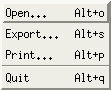
\includegraphics {./include/exit.pdf}}
%\makebox[\textwidth]{\framebox[5cm]{\rule{0pt}{5cm}}}
\caption{Exit the System} \label{fig:exitSys}
\end{figure}
\end{comment}

\subsection{Changing the ``Type''}

Often one will frequently change between the solution diagram and the bifurcation diagram.
The ``Type'' menu helps to complete this change. This menu includes two
items, ``Solution'', and ``Bifurcation''. There is a marker beside the current
diagram. For example, if the current diagram is the solution diagram, 
but we want to change to the bifurcation diagram, 
we can do so by clicking ``Type $\to$ Bifurcation'' to switch to the
bifurcation diagram. 

\begin{figure}[!htb]
    \begin{minipage}[b]{0.5\textwidth}
        \begin{center}
        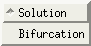
\includegraphics {./include/typeMenu.pdf}
        \caption{The Type Menu} \label{fig:tpyeMenu}
	\end{center}
    \end{minipage}%
    %\hspace{0.0\textwidth}%
    \begin{minipage}[b]{0.5\textwidth}
        \begin{center}
        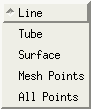
\includegraphics {./include/styleMenuNew.pdf}
        \caption{The Style Menu} \label{fig:styleMenu}
	\end{center}
    \end{minipage}
\end{figure}

\subsection{Changing the ``Style''}

\PLAUT~ provides four ways to draw the graphics, \textit{i.e.}, using 
curves, tubes, points, or as a surface. One can select the style from 
the ``Style'' menu. The ``Style'' menu is shown in Figure \ref{fig:styleMenu}.

\subsection{Coordinate axes} 

Figure \ref{fig:coordMenu} shows the selections of the ``Coord'' menu.
One may use this menu to select to show or not to show 
coordinate axes, and the type of coordinate axes, in the graphics.

\subsection{Options}

The ``Options'' Menu provides functions to add or remove widgets from the graphics.
It also allows to start/stop solution or orbit animation.
The ``normalize data'' normalizes the raw data to [0,1]. 
``Preference'' lets  us set preferences for the GUI (see Figure \ref{fig:optionMenu}). 
\begin{figure}[!htb]
	\centering
    \begin{minipage}[b]{0.5\textwidth}
        \centering
        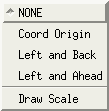
\includegraphics {./include/drawCoordMenu.pdf}
        \caption{The Draw-Coordinate-Axes Menu} \label{fig:coordMenu}
    \end{minipage}%
    %\hspace{0.2\textwidth}%
    \begin{minipage}[b]{0.5\textwidth}
        \centering
        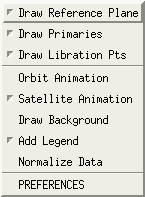
\includegraphics {./include/optionMenu.pdf}
    	\caption{The Options Menu} \label{fig:optionMenu}
    \end{minipage}
\end{figure}

\subsection{CR3BP animation}

The ``Center'' Menu allows to animate the motion of the three bodies in different
coordinate systems. We can animate the motion in a large-primary-centered inertial 
coordinate system, or in a small-primary-centered inertial system, or in the bary-centered
inertial system. Figure \ref{fig:centerMenu} displays the layout of the ``Center'' menu. 

\begin{figure}[!htb]
\centering
    \begin{minipage}[b]{0.5\textwidth}
        \centering
        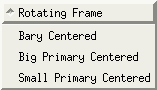
\includegraphics {./include/centerMenu.pdf}
        \caption{The Center Menu} \label{fig:centerMenu}
    \end{minipage}%
    %\hspace{0.2\textwidth}%
    \begin{minipage}[b]{0.5\textwidth}
        \centering
        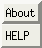
\includegraphics {./include/helpMenu.pdf}
        \caption{The Help Menu} \label{fig:helpMenu}
    \end{minipage}
\end{figure}


\subsection{Help}

The ``Help'' menu provides an on-line help on how to use \PLAUT.

\subsection{Picking a point in the diagram}

The picking operation is useful when we want to know data corresponding to a certain
point in the diagram. In order to execute a picking operation, we should follow these steps.
\begin{itemize}
	\item Click the arrow icon to change the mouse to picking state. 
    \item Move the mouse to the point of interest.
	\item Click the left button of the mouse to pick the point.
\end{itemize}

Once a point has been picked, a new window is popped up. In this new window, the Floquet
multipliers of the point are shown in an x-y plane.  
Black crosses in the diagram indicate the Floquet Multipliers.
The solution, and the values of the corresponding Floquet Multipliers, are given in the lower part of the
window. A unit circle is drawn in the diagram.
Figure \ref{fig:flq} is an example of the picking operation.
From this diagram, we can see that two Floquet Multipliers
are outside the unit circle, two are on the unit circle, and the other two are inside the unit circle.

\begin{figure}[!htb]
\centering
\scalebox{.60}{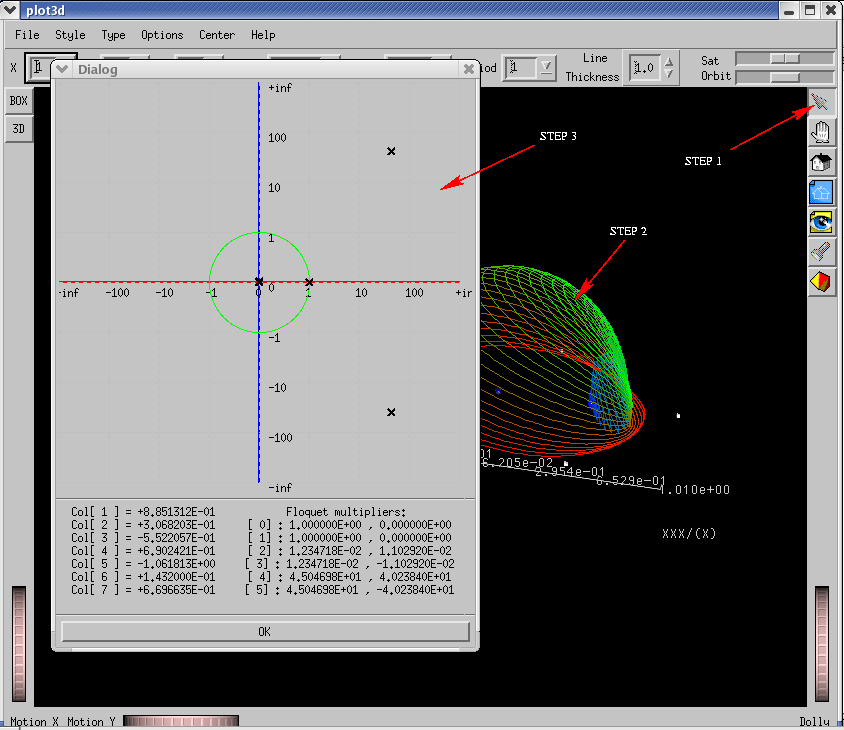
\includegraphics {./include/floquet.pdf}}
%\makebox[\textwidth]{\framebox[5cm]{\rule{0pt}{5cm}}}
\caption{Picking a point }
\label{fig:flq}
\end{figure}

\subsection{Choosing the variables}

\begin{figure}[!htb]
\centering
\scalebox{.60}{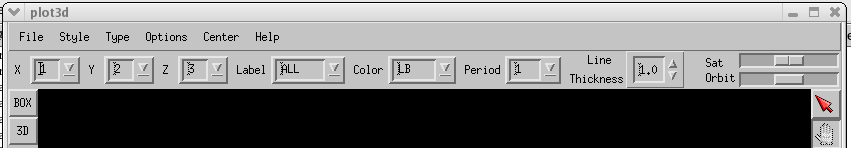
\includegraphics {./include/menubar.pdf}}
%\makebox[\textwidth]{\framebox[5cm]{\rule{0pt}{5cm}}}
\caption{Menu-bar layout}
\label{fig:mnbar}
\end{figure}

AUTO can generate large amounts of data. The CR3BP, for example, has 6 variables, \textit{i.e.}, $x,y,
z, x', y', z'$, and time. One can choose to draw any combination of these variables in 2  
or 3 dimensions using \PLAUT. On the list bar,  
we can see three {dropdown lists} with label ``X'', ``Y'', and ``Z'' (See Figure~\ref{fig:mnbar}).
Each of these three lists has the exact number of choices, namely, the number of variables of the system plus one.
In our case, these lists have 7 choices, which are represented by the integers 0 to 6. 
0 represents time. 1 to 6 stand for $x, y, z, x', y'$, and $z'$, respectively. 
``1'' is selected for ``X'', which indicates that $x$ is drawn on the X-axis. 
``2'' is selected for ``Y'',  which indicates that $y$ is represented on the Y-axis. 
``3'' is selected for ``Z'',  which indicates that $z$ is represented on the Z-axis. 

\begin{figure}[!htb]
\centering
\scalebox{.50}{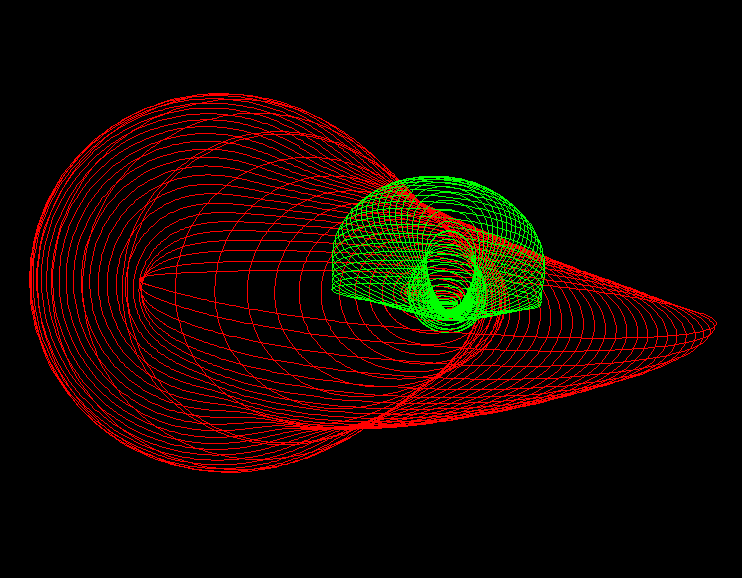
\includegraphics {./include/2component.pdf}}
%\makebox[\textwidth]{\framebox[5cm]{\rule{0pt}{5cm}}}
\caption{Displaying multiple components}
\label{fig:twoPairs}
\end{figure}

We can also show multiple combinations at the same time. For example, if we want 
to show x-y-z and x'-y'-z' in the same diagram, we can input $1,4$ in the ``X'' \textrm{dropdown list} to 
select $x$ and $x'$ being drawn on the X-axis, input $2,5$ in the ``Y'' list to show $y$ and $y'$ on the Y-axis,
and input $3,6$ in the ``Z'' \textrm{dropdown list} to draw $z$ and $z'$ on the Z-Axis. Note that after finishing 
the input in the \textrm{dropdown list} box, we must type ``ENTER'' for  
the input to be accepted by the system. Figure \ref{fig:twoPairs} shows the results of the above
choices. The combination is flexible. For example, if X is $1$, Y is $3, 5$, and Z is $4, 5, 6$, 
the system will automatically reorganize them to $1-3-4$, $1-5-5$, $1-3-6$ and show the results.
If X is $1, 5$,  Y is $2$, and Z is $3, 4$, the system reorganizes them to $1-2-3$, $5-2-4$.

Different components are drawn with different colors from blue to red. 

The default values can be set in the resource file. If no resource file exists, then the system
will use ``1'' for X-axis, ``2'' for Y-axis, and ``3''for Z-axis for both the solution and the bifurcation
diagrams.

\subsection{Choosing labels}

From the Label list, we can choose the label of the solution to be drawn. If ``ALL'' is chosen, all 
solutions are shown in the diagram. If ``NONE'' is chosen, none of the solutions is shown.
``HALF'' shows the solutions with odd labels and special solutions only. ``SPEC'' lets the system
show the special solutions only.
We can also show selected solutions by inputting their labels in the list
box separated by commas. 
For example, typing 1, 10, 15, 20 will lead the system to show only the solutions with label 1, 10, 15 and 20. 

We can set the default value for this list in the \PLAUT~resource file.

\subsection{Coloring}

Many coloring methods are provided. They can be classified into three groups. The first group
is coloring by variables. 
This group provides as many choices as the number of variables of a problem plus
1 for the time. 
The second group is coloring by parameters. These parameters are defined by the AUTO user. 
in the AUTO constants file. 
There are as many choices as the number of parameters defined in the AUTO constants file.
The third group includes ``TYPE'', type of solution, 
``PONT'', point number, 
``BRAN'', the branch to which the solution belongs, 
and ``LABL'', label of the solution. 
Different coloring methods cannot be used at the same time.
Figure \ref{fig:clrMethod} shows the difference between coloring by type and coloring by label. 
From Figure \ref{fig:clrMethod}(a), we can see that there is only one
branching orbit in this family, which is shown in cyan. 
In Figure~\ref{fig:clrMethod}(b), the start solution is colored in blue, and the last solution is colored in red. 
When using time to color the diagram, 0 is set to blue, while 1 is set to red. 
\begin{figure}[!htb]
    \subfigure[Coloring by ``Type'']{
    \label{fig:clrType}
    \begin{minipage}[b]{0.32\textwidth}
        \centering
        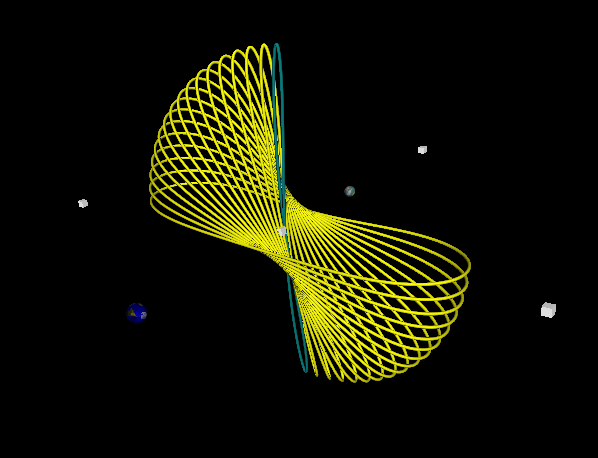
\includegraphics[width=5.0cm, height=5.0cm] {./include/clrTyMu0.pdf}
    \end{minipage}}%
    \subfigure[Coloring by ``Label'']{
    \label{fig:clrLabel}
    \begin{minipage}[b]{0.32\textwidth}
        \centering
        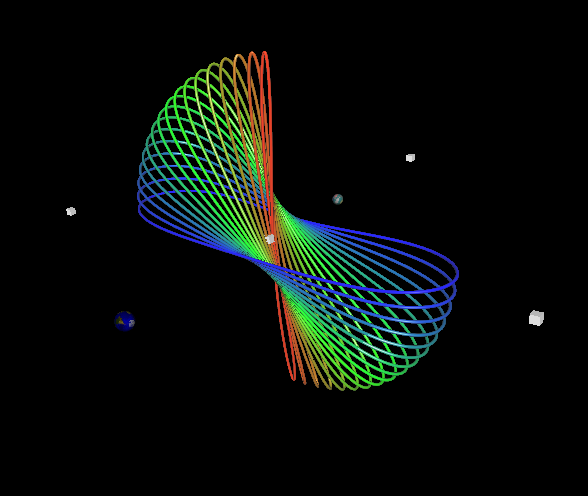
\includegraphics[width=5.0cm, height=5.0cm]{./include/clrLBMu0.pdf}
    \end{minipage}}%
    \subfigure[Coloring by ``Time'']{
    \label{fig:clrTime}
    \begin{minipage}[b]{0.32\textwidth}
        \centering
        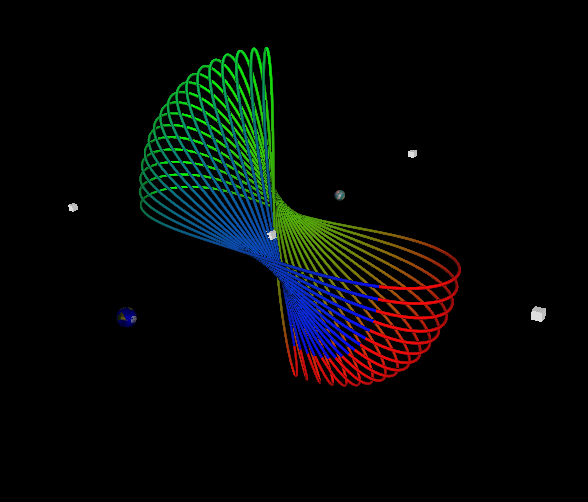
\includegraphics[width=5.0cm, height=5.0cm]{./include/clrTimeMu0.pdf}
    \end{minipage}}
    \caption{Coloring} \label{fig:clrMethod}
\end{figure}

We can set the default value in the \PLAUT~resource file.

\subsection{Number of periods to be animated}

Generally only one period is animated when we animate the solution in the inertial frame.
However, the SpinBox allows us to change the default value. 
 This is a specially designed function for the CR3BP. 
It is useful when  we animate the motion in the three bodies in the inertial frame.

\subsection{Changing the line/tube thickness}

The ``Line Thickness'' spinbox allows us to increase or decrease the line/tube thickness
in the diagram.  The \PLAUT~ resource file also provides a way to change the default values of the
line/tube thickness.

\subsection{Changing the animation speed}

The ``Sat'' and ``Orbit'' scale bar allow us to change the animation speed. 
Their Maximum and Minimum value can be set in the resource file.

\subsection{Changing the background picture}

A user can set the background with his favorite picture. 
To do this, a user should copy the picture to the directory ``\$AUTO\_DIR/plaut04/widgets'', 
and then change the name of the file to ``background.rgb''.

\section{Setting up the resource file}

The \PLAUT~resource file sets default values for 
almost all controls of \PLAUT. 
%Generally when we solve a problem, we want
%to put the solutions in the same directory. 
%For the same problem, what a user is interested in is almost the same.  
\PLAUT~allows us to write our own resources files and put them in the same directory as the AUTO data files. 
\PLAUT~first looks for the resource file in the current directory.
If it cannot find a resource file there, then it will try to use the one installed
in the AUTO root directory. If both these searches fail, then the internal
default values will be used.

In order to write a usable resource file, one should follow the following rules:
\begin{enumerate}
\item Comment lines start with ``\#''. Comments may take as many lines as desired.
\item Between the ``variable name'' and the default value, we must use 
``='' to tell the system that the left side is the ``variable name'', and
the right side is its corresponding default value.
\item If a ``variable'' has aggregate values, a comma ``,'' must be used between
two values.
\item The line type is set using 4-digit hexadecimals, starting with ``0x''. Its values can 
range from $0$ (invisible) to ``0xffff'' (solid). The system default is ``0xffff'' for stable
solutions, and ``0x3333'' for unstable ones. 
The line pattern is determined by the number of $1$s and $0$s when the hexadecimal
is converted to a $16$-bit binary. A ``$1$'' indicates that the drawing occurs, and ``$0$'' that 
it does not, on a pixel by pixel basis. For example, the pattern ``0xAAAA'', 
in binary is $0000100010001000$, and \PLAUT~interprets this as drawing 
3 bits off, 1 bit on, 3 bits off, 1 bit on, 3 bits off, 1 bit on and finally 4 bits off.
The pattern is read backward because the low order bits are used first.
\item Some variables can only be set to ``Yes'' or ``No''. They cannot be assigned other values.
\item No ``variable name'' should be  modified.
\end{enumerate}

It is strongly recommended that the default resource file is used as a template
when writing a custom resource file. 

Below is a copy of the default resource file. 
{\footnotesize
\begin{verbatim}
#version 0.0

# Line colors are represented by RGB values from 0 to 1.0.
# DEFAULT color is also used when animationLabel == 0, i.e.,
# when showing all solutions and animating the solution change.
# Point Type    RED  GREEN  BLUE PATTERN
DEFAULT       = 1.0,  1.0,  1.0, 0xffff
BP ALG        = 1.0,  0.0,  0.0, 0xffff
LP ALG        = 0.0,  1.0,  0.0, 0xffff
HB            = 0.0,  0.0,  1.0, 0xffff
UZ4           = 1.0,  1.0,  0.0, 0xffff
UZ-4          = 0.5,  0.5,  0.0, 0xffff
LP DIF        = 0.0,  0.0,  0.5, 0xffff
BP DIF        = 0.0,  0.5,  0.5, 0xffff
PD            = 1.0,  0.0,  1.0, 0xffff
TR            = 0.0,  1.0,  1.0, 0xffff
EP            = 0.3,  0.0,  0.3, 0xffff
MX            = 0.6,  0.0,  0.6, 0xffff
OTHERS        = 1.0,  1.0,  1.0, 0xffff

# Initialize the line pattern for showing stability:
UNSTABLE LINE PATTERN = 0xffff 
STABLE LINE PATTERN   = 0xffff

# Initialize the default options:
Draw Reference Plane  = No
Draw Reference Sphere = No
Orbit Animation       = No
Satellite Animation   = No 
Draw Primaries        = No 
Draw Libration Points = No 
Normalize Data        = No
Draw Labels           = No
Show Label Numbers    = No
Draw Background       = No
Draw Legend           = No

# Initialize the default coordinate axes:
#  0 --- None,
#  1 --- at origin
#  2 --- at left and behind
#  3 --- at left and ahead
#  4 --- always at origin
Coordinate Type = 3

# Draw Scale on the Aexs
Draw Scale = Yes 

#  Initialize the default graph type:
#  0 --- Solution (fort.8)
#  1 --- Bifurcation (fort.7)
Graph Type    = 0

# Initialize the default graph style:
#  0 --- LINES,
#  1 --- TUBES,
#  2 --- SURFACE
Graph Style  =  0

# Set the window width and height:
Window Width        = 1000
Window Height       = 1000 

# Set X, Y, Z axes for the solution diagram:
# 0 is Time for X,Y,Z.
X Axis Solution             = 1
Y Axis Solution             = 2
Z Axis Solution             = 3

# Set X, Y, Z axes for the bifurcation diagram:
X Axis Bifurcation          = 4
Y Axis Bifurcation          = 5
Z Axis Bifurcation          = 6

#Labeled solutions:
Labels              = 0

# Set coloring method:
# -6 --- STABILITY
# -5 --- POINT
# -4 --- BRANCH
# -3 --- TYPE 
# -2 --- LABEL 
# -1 --- COMPONENT 
# Otherwise, according to the data in the ith column of the solution file.
# It can only be set to an integer value.
#Coloring Method           = -3
# For the solution diagram:
Coloring Method Solution  = -3
# For the bifurcation diagram:
Coloring Method Bifurcation = -3
Number of Period Animated = 1

# Line Width Scaler adjusts the thickness of curves:
Line Width Scaler         = 1.0

# The AniLine Thickness Scaler sets the thickness of animated solution curves:
AniLine Thickness Scaler  = 3.0

# Background color:
Background Color  = 0.0,  0.0,   0.0

# Background transparency:
Background Transparency = 0.0 

# Set the radius of the spheres used for labels:
# The normal size is 1.0.
# For smaller radius, use 0.xxx
# For bigger radius, use  X.XXX
Label Sphere Radius       =  1.0

# Disk Rotation
Disk Rotation = 1.0, 0.0, 0.0, 1.570796

# Disk Position
Disk Position = 0.0, 0.0, 0.0

# Disk Radius
Disk Radius = 1.0

# Disk Height
Disk Height = 0.001

# Disk Transparency [0, 1]
Disk Transparency = 0.7 
 
# Read Disk From File
Disk From File = No 
 
# Sphere Position
Sphere Position = 0.0, 0.0, 0.0

# Sphere Radius
Sphere Radius = 1.0

# Sphere Transparency [0, 1]
Sphere Transparency = 0.7

# Read Sphere From File
Sphere From File = No

# Axes color:
X Axis Color    = 1.0,  0.0,   0.0
Y Axis Color    = 0.0,  1.0,   0.0
Z Axis Color    = 0.0,  0.0,   1.0

# Color of the satellite, large primary, and small primary in animation:
satellite Color             = 1.0,  0.0,   0.0
large primary Color         = 0.0,  1.0,   0.0
large primary tail Color    = 0.0,  1.0,   1.0
small primary Color         = 0.0,  0.0,   1.0
small primary tail Color    = 0.5,  0.5,   0.0

# Surface color:
Surface Color         =  0.0,  1.0,  0.0

# Stable solution color:
Stable Solution Color = 0.0, 0.0, 1.0

# Stable solution color:
Unstable Solution Color = 1.0, 0.0, 0.0

# Set the radius of the satellite, large primary, and small primary:
# The normal size is 1.0.
# For smaller radius, use 0.xxx
# For bigger radius, use  X.XXX
Satellite Radius        = 1.0
Large Primary Radius    = 1.0
Small Primary Radius    = 1.0
Libration Point Size    = 1.0

# Set the initial, maximum and minimum satellite animation speed:
Sat Animation Speed = 100
Sat Max Animation Speed = 100
Sat Min Animation Speed = 0

# Set the initial, maximum and minimum orbit-change animation speed:
Orbit Animation Speed = 50
Orbit Max Animation Speed = 100
Orbit Min Animation Speed = 0

# Set the active AUTO parameter indices:
parameter ID = 10

# Choose 3D or 2D graph:
#3D  = Yes 

# Choose 3D or 2D graph for the bifurcation diagram:
3DBif = Yes

# Choose 3D or 2D graph for the solution diagram:
3DSol = Yes

\end{verbatim}
}

\section{Example}

In this example, we want to view a CR3BP data set.
We want the diagram to show the ``$x$'' component on the X-axis, ``$y$'' component on the Y-axis, and ``$z$'' component on the Z-axis
for the solution diagram. 
%and column 4 of the AUTO b file as the X-axis, column 5
%on the Y-axis, and column 6 on the Z-axis, for the bifurcation diagram. 
In the CR3BP, we use the parameters ``1 2 3 10 21 22 23'' in the AUTO  
calculations, and we also want to be able to use these to color the diagram, so we set the ``parameter indices''.  

Other preferences include
\begin{itemize}
\item The diagram is drawn using Tubes.
\item Coordinate axes are not drawn.
\item No animation.
\item Reference plane, libration points, and primaries are drawn.
\item All labels are shown.
\item Data is not normalized. 
\end{itemize}

The settings are the settings in the resource file are then as follows:
{\footnotesize
\begin{verbatim}
#  Initialize the default options
Draw Reference Plane  = Yes
Orbit Animation       = No
Satellite Animation   = No 
Draw Primaries        = Yes
Draw Libration Points = Yes
Normalize Data        = No
Draw Background       = No

#  Initialize the default graph type
#  0 --- Solution(fort.8)  1 --- Bifurcation(fort.7)
Graph Type    = 0

# initialize the default graph style
#  0 --- LINES,  1 --- TUBES, 2 ---- SURFACE  3--- nurbs curve
graph Style  =  1

# set X, Y, Z, and Label
# 0 is Time for X,Y,Z. 0 is "All" for Label

Solution X Axis              = 1
Solution Y Axis              = 2
Solution Z Axis              = 3

Labels                       = 0

#set the parameter indices 
parameter ID = 1,  2,  3, 10,  15, 21, 22,  23
\end{verbatim}
}

Based on the above settings, 
the solution diagram for the CR3BP family \L{1} for $\mu=0.01215$ appears in Figure \ref{fig:AppEx1}.

\begin{comment}
\begin{figure}[!htb]
	\centering
	%\includegraphics[width=10cm] {./include/ex1Mu0.01215V1.pdf}
	%\includegraphics[width=10cm] {./include/emV4Surface.pdf}
	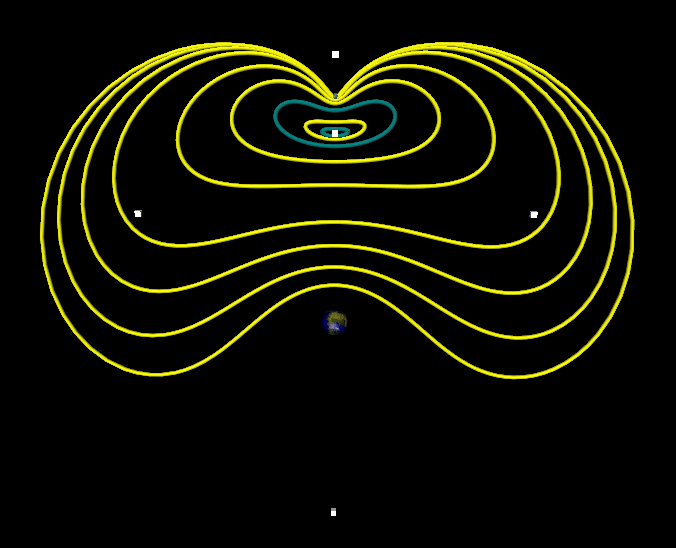
\includegraphics[width=10cm] {./include/emL1Sol.pdf}
%\makebox[\textwidth]{\framebox[5cm]{\rule{0pt}{5cm}}}
	\caption{Example}
\label{fig:AppEx1}
\end{figure}
\end{comment}

\begin{figure}[!htb]
        \centering
		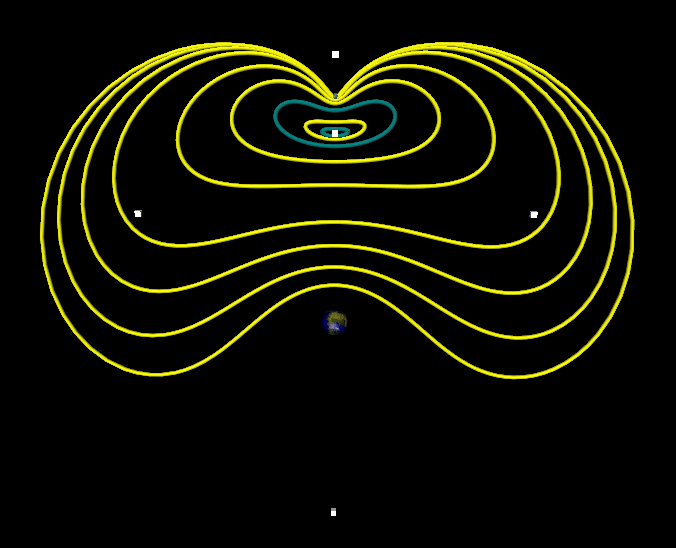
\includegraphics[width=10cm, height=10cm] {./include/emL1Sol.pdf}
        \caption{Example} \label{fig:AppEx1}
\end{figure}


%==============================================================================
%==============================================================================
\chapter{ The Graphical User Interface GUI94.} \label{ch:GUI}
%==============================================================================
%==============================================================================
\section{ General Overview.} \label{sec:GUI_Overview}
The {\cal AUTO} graphical user interface (GUI) is a tool
for creating and editing equations-files and constants-files;
see Section~\ref{ch:User_supplied_files}
 for a description of these files.
The GUI can also be used to run {\cal AUTO} and to manipulate and plot
output-files and data-files; 
see Section~\ref{sec:command_mode} for corresponding commands.
To use the GUI for a new equation, change to an empty work directory.
For an existing equations-file, change to its directory.
({\it Do not activate the GUI in the directory {\tt auto/07p} 
or in any of its subdirectories.})
Then type 

\centerline { @{\it auto}, }

or its abbreviation @{\it a}.
Here we assume that the {\cal AUTO} aliases have been activated; 
see Section~\ref{sec:Installation}.
The GUI includes a window for editing the equations-file,
and four groups of buttons, namely,
the {\it Menu Bar} at the top of the GUI,
the {\it Define Constants}-buttons at the center-left,
the {\it Load Constants}-buttons at the lower left,
and the {\it Stop- and Exit}-buttons.

{\bf Note :}~
Most GUI buttons are activated by point-and-click action with 
the {\it left} mouse button. 
If a beep sound results then the {\it right} mouse button must be used. 

\subsection{ The Menu bar.}
It contains the main buttons for running {\cal AUTO}
and for manipulating the equations-file, the constants-file,
the output-files, and the data-files.
In a typical application, these buttons are used from left to right.
First the {\it Equations} are defined and, if necessary, {\it Edited},
before being {\it Written}.
Then the {\cal AUTO}-constants are {\it Defined}.
This is followed by the actual {\it Run} of {\cal AUTO}.
The resulting output-files can be {\it Saved} as data-files,
or they can be {\it Appended} to existing data-files.
Data-files can be {\it Plotted} with the graphics program {\cal PLAUT},
and various file operations can be done with the {\it Files}-button.
Auxiliary functions are provided by the {\it Demos-}, {\it Misc-},
and {\it Help}-buttons.
The Menu Bar buttons are described in more detail 
in Section~\ref{sec:GUI_Menu_bar}.


\subsection{ The Define-Constants-buttons.}
These have the same function as
the {\it Define}-button on the  Menu Bar, namely to set and change
{\cal AUTO}-constants.
However, 
for the {\it Define}-button all constants appear in one panel, 
while 
for the Define Constants-buttons they
are grouped by function, 
as in Chapter~\ref{ch:AUTO_constants}, namely
{\it Problem} definition constants,
{\it Discretization} constants,
convergence {\it Tolerances},
continuation {\it Step Size},
diagram {\it Limits},
designation of free {\it Parameters},
constants defining the {\it Computation},
and
constants that specify {\it Output} options.


\subsection{ The Load-Constants-buttons.}
The {\it Previous}-button can be used to load an existing {\cal AUTO}-constants file.
Such a file is also loaded, if it exists,
by the {\it Equations}-button on the {\it Menu Bar}.
The {\it Default}-button can be used
to load  default values of all {\cal AUTO}-constants. 
Custom editing is normally necessary.


\subsection{ The Stop- and Exit-buttons.}
The {\it Stop}-button can be used to abort execution of an {\cal AUTO}-run.
This should be done only in exceptional circumstances.
Output-files, if any, will normally be incomplete and should be deleted.
Use the {\it Exit}-button to end a session.


\section{ The Menu Bar.} \label{sec:GUI_Menu_bar}
\subsection{ Equations-button.}
This pull-down menu contains the items
{\it Old}, to load an existing equations-file,
{\it New}, to load a model equations-file,
and
{\it Demo}, to load a selected demo equations-file.
Equations-file names are of the form {\tt xxx.f}.
The corresponding constants-file {\tt c.xxx} is also loaded if it exists.
The equation name {\tt xxx} remains active until redefined.

\subsection{ Edit-button.}
This pull-down menu contains the items
{\it Cut} and {\it Copy}, 
to be performed on text in the GUI window
highlighted by click-and-drag action of the mouse,
and the item {\it Paste}, which places editor buffer text at the
location of the cursor.



\subsection{ Write-button.}
This pull-down menu contains the item
{\it Write},
to write the loaded files {\tt xxx.f} and {\tt c.xxx},
by the active equation name,
and the item
{\it Write As}
to write these files by a selected new name, which then becomes the active name.


\subsection{ Define-button.}
Clicking this button will display the full {\cal AUTO}-constants panel.
Most of its text fields can be edited,
but some have restricted input values that can be selected with
the right mouse button.
Some text fields will display a subpanel for entering data.
To actually apply changes made in the panel, click the
{\it OK-} or {\it Apply}-button at the bottom of the panel.



\subsection{ Run-button.}
Clicking this button will write the constants-file {\tt c.xxx} and run {\cal AUTO}.
If the equations-file has been edited then it should first be rewritten 
with the {\it Write}-button. 


\subsection{ Save-button.}
This pull-down menu contains the item
{\it Save},
to save the output-files {\tt fort.7}, {\tt fort.8}, {\tt fort.9},
as {\tt b.xxx}, {\tt s.xxx}, {\tt d.xxx}, respectively.
Here {\tt xxx} is the active equation name.
It also contains the item
{\it Save As}, 
to save the output-files under another name. 
Existing data-files with the selected name, if any, will be overwritten.


\subsection{ Append-button.}
This pull-down menu contains the item
{\it Append},
to append the output-files {\tt fort.7}, {\tt fort.8}, {\tt fort.9},
to existing data-files {\tt b.xxx}, {\tt s.xxx}, {\tt d.xxx}, respectively.
Here {\tt xxx} is the active equation name.
It also contains the item
{\it Append To}, 
to append the output-files to other existing data-files.

\subsection{ Plot-button.}
This pull-down menu contains the items
{\it Plot},
to run the plotting program {\cal PLAUT} for the data-files 
{\tt b.xxx} and {\tt s.xxx},
where {\tt xxx} is the active equation name,
and the item
{\it Name}, 
to run {\cal PLAUT} with other data-files.


\subsection{ Files-button.}
This pull-down menu contains 
the item 
{\it Restart}, to redefine the restart file.
Normally, when restarting from a previously computed solution,
the restart data is expected in the file {\tt s.xxx},
where {\tt xxx} is the active equation name.
Use the {\it Restart}-button to read the restart data from another data-file
in the immediately following run.  
The pull-down menu also contains the following items~:
\begin{itemize}
\item[-]{\it Copy},~ to copy  
  {\tt b.xxx}, {\tt s.xxx}, {\tt d.xxx}, {\tt c.xxx},
  to
  {\tt b.yyy}, {\tt s.yyy}, {\tt d.yyy}, {\tt c.yyy}, resp.;

\item[-]{\it Append},~ to append data-files
  {\tt b.xxx}, {\tt s.xxx}, {\tt d.xxx},
  to
  {\tt b.yyy}, {\tt s.yyy}, {\tt d.yyy}, resp.;

\item[-]{\it Move},~ to move 
  {\tt b.xxx}, {\tt s.xxx}, {\tt d.xxx}, {\tt c.xxx},
  to
  {\tt b.yyy}, {\tt s.yyy}, {\tt d.yyy}, {\tt c.yyy}, resp.;

\item[-]{\it Delete},~ to delete data-files
  {\tt b.xxx}, {\tt s.xxx}, {\tt d.xxx};  

\item[-]{\it Clean}, to delete all files of the form 
  {\tt fort.*}, {\tt *.o}, and {\tt *.exe}.  
\end{itemize}


\subsection{ Demos-button.}
This pulldown menu contains the items
{\it Select},
to view and run a selected {\cal AUTO} demo in the demo directory,
and
{\it Reset},
to restore the demo directory to its original state.
Note that demo files can be copied to the user work directory
with the {\it Equations/Demo}-button.


\subsection{ Misc.-button.}
This pulldown menu contains the items
{\it Tek Window}
and
{\it VT102 Window},
for opening windows;
{\it Emacs}
and
{\it Xedit},
for editing files,
and
{\it Print}, for printing the active equations-file {\tt xxx.f}.


\subsection{ Help-button.}
This pulldown menu contains the items
{\it {\cal AUTO}-constants}, for help on {\cal AUTO}-constants,
and
{\it User Manual}, for viewing the user manual; i.e., this document.


\section{ Using the GUI.} \label{sec:Using_the_GUI}
{\cal AUTO}-commands are described in Section~\ref{sec:command_mode} and
illustrated in the demos.
In Table~\ref{tbl:CM_GUI} we list the main {\cal AUTO}-commands 
together with the corresponding GUI button.

\begin{table}[htbp]
\begin{center}
\begin{tabular}{| l | l |}
\hline
{\it @r }  & {\it Run} \\  
\hline
{\it @sv }  & {\it Save}  \\ 
\hline
{\it @ap }  & {\it Append} \\ 
\hline
{\it @p }  & {\it Plot}  \\ 
\hline
{\it @cp }  & {\it Files/Copy}  \\ 
\hline
{\it @mv }  & {\it Files/Move}  \\ 
\hline
{\it @cl }  & {\it Files/Clean} \\ 
\hline
{\it @dl }  & {\it Files/Delete} \\  
\hline
{\it @dm }  & {\it Equations/Demo} \\  
\hline
\end{tabular}
\caption{Command Mode - GUI correspondences.}
\label{tbl:CM_GUI}
\end{center}
\end{table}


The {\cal AUTO}-command {\it @r xxx yyy} is given in the GUI as follows~:
click {\it Files/Restart} and enter {\it yyy} as data.
Then click {\it Run}.
As noted in Section~\ref{sec:command_mode}, 
this will run {\cal AUTO} with the current equations-file
{\tt xxx.f} and the current constants-file {\tt c.xxx}, 
while expecting restart data in {\tt s.yyy}.
The {\cal AUTO}-command {\it @ap xxx yyy} is given in the GUI by
clicking {\it Files/Append}.

\section{ Customizing the GUI.} \label{sec:Customizing_the_GUI}
\subsection{ Print-button.}
The {\it Misc/Print}-button on the Menu Bar can be customized 
by editing the file {\tt GuiConsts.h} in directory {\tt auto/07p/include}.

\subsection{ GUI colors.}
GUI colors can be customized by creating an X resource file.
Two model files can be found in directory {\tt auto/07p/gui}, namely,
{\tt Xdefaults.1} and {\tt Xdefaults.2}.
To become effective, edit one of these, if desired,
and copy it to {\tt .Xdefaults} in your home directory.
Color names can often be found in the system file {\tt /usr/lib/X11/rgb.txt}.

\subsection{ On-line help.}
The file {\tt auto/07p/include/GuiGlobal.h}
contains on-line help on {\cal AUTO}-constants and demos.
The text can be updated, subject to a modifiable maximum length.
On SGI machines this is 10240 bytes,
which can be increased, for example, to 20480 bytes, 
by replacing the line
{\it CC = cc -Wf, -XNl10240 -O}
in {\tt auto/07p/gui/Makefile} by
{\it CC = cc -Wf, -XNl20480 -O}
On other machines, the maximum message length is the system defined maximum
string literal length.


%==============================================================================
%==============================================================================
\chapter{ Description of {\cal AUTO}-Constants.} \label{ch:AUTO_constants}
%==============================================================================
%==============================================================================
\section{ The {\cal AUTO}-Constants File.} \label{sec:The_AUTO_constants_file}
As described in Section~\ref{ch:User_supplied_files}, 
if the equations-file is {\tt xxx.f} 
then the constants that define the computation 
are normally expected in the file  {\tt c.xxx}.
The general format of this file is the same for all {\cal AUTO} runs.
For example, the file {\tt c.cusp} 
in directory {\tt auto/07p/demos/cusp} is listed below.
(The tutorial demo {\tt cusp} is described in detail in 
Chapter~\ref{ch:Demos:_Tutorial}.)  

\begin{verbatim}
1 1 0 1                 NDIM,IPS,IRS,ILP
2 2 1                   NICP,(ICP(I),I=1,NICP)
5 4 3 2 1 0 0 0         NTST,NCOL,IAD,ISP,ISW,IPLT,NBC,NINT
200 -2. 2. 0 100        NMX,RL0,RL1,A0,A1
20 0  2 8 5 3 0         NPR,MXBF,IID,ITMX,ITNW,NWTN,JAC
1.e-6 1.e-6 0.0001      EPSL,EPSU,EPSS
0.01 0.005 0.1 1        DS,DSMIN,DSMAX,IADS
0                       NTHL,((I,THL(I)),I=1,NTHL)
0                       NTHU,((I,THU(I)),I=1,NTHU)
0                       NUZR,((I,UZR(I)),I=1,NUZR)
\end{verbatim}

The significance of the {\cal AUTO}-constants, grouped by function, is 
described in the sections below. 
Representative demos that illustrate use of the {\cal AUTO}-constants
are also mentioned.

%=====================================================================
\section{ Problem Constants.} \label{sec:Problem_constants}
\subsection{\tt NDIM} \label{sec:NDIM}
 Dimension of the system of equations as specified in the user-supplied
 routine {\tt FUNC}.

\subsection{\tt NBC}  \label{sec:NBC}
 The number of boundary conditions as specified in the user-supplied
 routine {\tt BCND}. \\
(Demos {\tt exp}, {\tt kar}.)

\subsection{\tt NINT}  \label{sec:NINT}
 The number of integral conditions as specified in the user-supplied
 routine {\tt ICND}. \\ 
(Demos {\tt int}, {\tt lin}, {\tt obv}.)

\subsection{\tt JAC}  \label{sec:JAC}
 Used to indicate whether derivatives are supplied by the user
 or to be obtained by differencing~:
\begin{itemize}
\item[-] {\tt JAC=0}~: 
  No derivatives are given by the user. (Most demos use {\tt JAC}=0.)
\item[-] {\tt JAC=1}~:  
  Derivatives with respect to state- and problem-parameters are given 
  in the user-supplied routines 
  {\tt FUNC}, {\tt BCND}, {\tt ICND} and {\tt FOPT}, where 
  applicable.  This may be necessary for sensitive problems. 
  It is also recommended for computations in which {\cal AUTO} generates 
  an extended system, for example, when {\tt ISW}=2.
  (For {\tt ISW} see Section~\ref{sec:ISW}.) \\
(Demos {\tt int}, {\tt dd2}, {\tt obt}, {\tt plp}, {\tt ops}.)
\end{itemize}
%=====================================================================
\section{ Discretization Constants.} \label{sec:Discretization_constants}
\subsection{\tt NTST}  \label{sec:NTST}
 The number of mesh intervals used for discretization.
 {\tt NTST} remains fixed during any particular run, but can be changed
 when restarting. 
 (For mesh adaption see {\tt IAD} in Section~\ref{sec:IAD}.)
 Recommended value of {\tt NTST} : As small as possible to maintain convergence. \\ 
 (Demos {\tt exp}, {\tt ab}, {\tt spb}.)


\subsection{\tt NCOL}  \label{sec:NCOL}
 The number of Gauss collocation points per mesh interval,
 (2 $\le$ {\tt NCOL} $\le$ 7).
 {\tt NCOL} remains fixed during any given run, but can be changed
 when restarting at a previously computed solution.
 The choice {\tt NCOL}=4, used in most demos, is recommended.
 If {\tt NDIM} is ``large'' and the solutions ``very smooth'' then
 {\tt NCOL}=2 may be appropriate.

\subsection{\tt IAD} \label{sec:IAD}
This constant controls the mesh adaption~: 
\begin{itemize}
\item[-] {\tt IAD=0}~:
  Fixed mesh. Normally, this choice should never be used, as it may result
  in spurious solutions. (Demo {\tt ext}.)
\item[-] {\tt IAD$>$0}~:  
  Adapt the mesh every {\tt IAD} steps along the family.
  Most demos use {\tt IAD=3}, which is the strongly recommended value.
\end{itemize}

When computing  ``trivial'' solutions to a boundary value problem,
for example, when all solution components are constant, then the
mesh adaption may fail under certain circumstances, and overflow may
occur. In such case, try recomputing the solution family with a fixed
mesh {\tt (IAD=0)}. Be sure to set  {\tt IAD} back to {\tt IAD=3} 
for computing eventual non-trivial bifurcating solution families.
%=====================================================================
\section{ Tolerances.} \label{sec:Tolerances}
\subsection{\tt EPSL}  \label{sec:EPSL}
 Relative convergence criterion for equation parameters in the Newton/Chord 
 method. Most demos use {\tt EPSL}=$10^{-6}$ or {\tt EPSL}=$10^{-7}$,
 which is the recommended value range.

\subsection{\tt EPSU}  \label{sec:EPSU}
 Relative convergence criterion for solution components in the Newton/Chord 
 method. Most demos use {\tt EPSU}=$10^{-6}$ or {\tt EPSU}=$10^{-7}$,
 which is the recommended value range.

\subsection{\tt EPSS}  \label{sec:EPSS}
 Relative arclength convergence criterion for the detection of special solutions. 
 Most demos use {\tt EPSS}=$10^{-4}$ or  {\tt EPSS}=$10^{-5}$,
 which is the recommended value range.
 Generally, {\tt EPSS} should be approximately 100 to 1000 times the value
 of {\tt EPSL}, {\tt EPSU}.
 
\subsection{\tt ITMX}  \label{sec:ITMX}
 The maximum number of iterations allowed in the accurate
 location of special solutions, such as bifurcations, folds, 
 and user output points, by M\"uller's method with bracketing.
 The recommended value is {\tt ITMX}=8, used in most demos.

\subsection{\tt NWTN}  \label{sec:NWTN}
 After {\tt NWTN} Newton iterations the Jacobian is frozen, i.e.,
 {\cal AUTO} uses full Newton for the first {\tt NWTN} iterations
 and the Chord method for iterations {\tt NWTN}+1 to {\tt ITNW}.
 The choice {\tt NWTN}=3 is strongly recommended and used in most demos.
 Note that this constant is only effective for ODEs, i.e., for solving
 the piecewise polynomial collocation equations.
 For algebraic systems {\cal AUTO} always uses full Newton.

\subsection{\tt ITNW}  \label{sec:ITNW}
 The maximum number of combined Newton-Chord iterations.
 When this maximum is reached, the step will be retried with 
 half the stepsize.
 This is repeated until convergence, or until the minimum
 stepsize is reached. In the latter case the computation of
 the family is discontinued and a message printed in {\tt fort.9}.
 The recommended value is {\tt ITNW}=5, but {\tt ITNW}=7 may be used for 
 ``difficult'' problems, for example, 
 demos {\tt spb}, {\tt chu}, {\tt plp}, etc.

%=====================================================================
\section{ Continuation Step Size.} \label{sec:step_size}
\subsection{\tt DS}  \label{sec:DS}
 {\cal AUTO} uses pseudo-arclength continuation for following solution families.
 The pseudo-arclength stepsize is the distance between
 the current solution and the next solution on a family.
 By default, this distance includes all state variables
 (or state functions) and all free parameters.
 The constant {\tt DS} defines the pseudo-arclength stepsize to be used for the
 first attempted step along any family. 
 (Note that if {\tt IADS}$>$0 then {\tt DS} will automatically be adapted
 for subsequent steps and for failed steps.)
 {\tt DS} may be chosen positive or negative; changing its sign 
 reverses the direction of computation.
 The relation {\tt DSMIN} $\le$ $\abs {\tt DS}$ $\le$ {\tt DSMAX} must be satisfied.
 The precise choice of {\tt DS} is problem-dependent; the demos use a value 
 that was found appropriate after some experimentation.
 

\subsection{\tt DSMIN}  \label{sec:DSMIN}
 This is minimum allowable absolute value of the pseudo-arclength 
 stepsize. {\tt DSMIN} must be positive.
 It is only effective if the pseudo-arclength step is adaptive,
 i.e., if {\tt IADS}$>$0.
 The choice of {\tt DSMIN} is highly problem-dependent;
 most demos use a value that was found appropriate after some
 experimentation.
 See also the discussion in Section~\ref{sec:Efficiency}.

\subsection{\tt DSMAX}  \label{sec:DSMAX}
 The maximum allowable absolute value of the pseudo-arclength stepsize.
 {\tt DSMAX} must be positive.
 It is only effective if the pseudo-arclength step is adaptive,
 i.e., if {\tt IADS}$>$0.
 The choice of {\tt DSMAX} is highly problem-dependent; 
 most demos use a value that was found appropriate after some
 experimentation.
 See also the discussion in Section~\ref{sec:Efficiency}.

\subsection{\tt IADS}  \label{sec:IADS}
This constant controls the frequency of adaption of the 
pseudo-arclength stepsize.
\begin{itemize}
\item[-] {\tt IADS=0}~: 
  Use fixed pseudo-arclength stepsize, i.e., the stepsize will
  be equal to the specified value of {\tt DS} for every step.
  The computation of a family will be discontinued as soon as
  the maximum number of iterations {\tt ITNW} is reached.
  This choice is not recommended. \\(Demo {\tt tim}.)
\item[-] {\tt IADS$>$0}~:  
 Adapt the pseudo-arclength stepsize after every {\tt IADS} steps.
  If the Newton/Chord iteration converges rapidly then 
  $\abs{\tt DS}$ will be increased, but never beyond {\tt DSMAX}.
  If a step fails then it will be retried with half
  the stepsize. This will be done repeatedly until the
  step is successful or until $\abs{\tt DS}$ reaches {\tt DSMIN}. 
  In the latter case nonconvergence will be signalled.
  The strongly recommended value is {\tt IADS}=1, which is used in 
  almost all demos.
\end{itemize}
  
\subsection{\tt NTHL}  \label{sec:NTHL}
By default, the pseudo-arclength stepsize includes all state variables
(or state functions) and all free parameters.
Under certain circumstances one may want to modify the weight accorded 
to individual parameters in the definition of stepsize.
For this purpose, {\tt NTHL} defines the number of parameters whose weight 
is to be modified.
If {\tt NTHL}=0 then all weights will have default value 1.0~.
If {\tt NTHL}$>$0 then one must enter {\tt NTHL} pairs,
             ~{\it Parameter Index} ~ {\it Weight}~,
with each pair on a separate line.

For example, for the computation of periodic solutions it is 
recommended that the period not be included in the pseudo-arclength 
continuation stepsize, in order to avoid period-induced limitations 
on the stepsize near orbits of infinite period. 
This exclusion can be accomplished by setting {\tt NTHL=1}, with, 
on a separate line, the pair ~ 11 ~ 0.0 ~.
Most demos that compute periodic solutions use this option;
see for example demo {\tt ab}.

\subsection{\tt NTHU}  \label{sec:NTHU}
Under certain circumstances one may want to modify the weight accorded 
to individual state variables (or state functions) in the definition 
of stepsize.
For this purpose, {\tt NTHU} defines the number of states whose weight 
is to be modified.
If {\tt NTHU}=0 then all weights will have default value 1.0~.
If {\tt NTHU}$>$0 then one must enter {\tt NTHU} pairs,
             ~{\it State Index} ~ {\it Weight}~,
with each pair on a separate line.
At present none of the demos use this option.
%=====================================================================
\section{ Diagram Limits.} \label{sec:Diagram_limits}

There are three ways to limit the computation of a family~:

\begin{itemize}
\item[-]
By appropriate choice of the computational window 
defined by the constants {\tt RL0}, {\tt RL1}, {\tt A0}, and {\tt A1}.
One should always check that the starting solution lies within
this computational window, otherwise the computation will stop immediately
at the starting point.

\item[-]
By specifying the maximum number of steps, {\tt NMX}.

\item[-]
By specifying a negative parameter index in the list associated 
with the constant {\tt NUZR}; see Section~\ref{sec:NUZR}. 
\end{itemize}

\subsection{\tt NMX} \label{sec:NMX}
The maximum number of steps to be taken along any family.

\subsection{\tt RL0}  \label{sec:RL0}
 The lower bound on the principal continuation parameter.
 (This is the parameter which appears first in the {\tt ICP} list;
 see Section~\ref{sec:ICP}.). 


\subsection{\tt RL1}  \label{sec:RL1}
 The upper bound on the principal continuation parameter. 

\subsection{\tt A0}  \label{sec:A0}
 The lower bound on the principal solution measure.
 (By default, if {\tt IPLT}=0, the principal solution measure
 is the $L_2$-norm of the state vector or state vector function.
 See the {\cal AUTO}-constant {\tt IPLT} in Section~\ref{sec:IPLT} 
 for choosing another principal solution measure.)

\subsection{\tt A1}  \label{sec:A1}
 The upper bound on the principal solution measure.

%=====================================================================
%=====================================================================
\section{ Free Parameters.} \label{sec:Free_parameters}


\subsection{\tt NICP, ICP}  \label{sec:ICP}
For each equation type and for each continuation calculation there is
a typical (``generic'') number of problem parameters that must be 
allowed to vary, in order for the calculations to be properly posed.
The constant {\tt NICP} indicates how many free parameters have been specified,
while the array {\tt ICP} actually designates these free parameters.
The parameter that appears first in the {\tt ICP} list is called the 
``principal continuation parameter''.
Specific examples and special cases are described below.

%=====================================================================
\subsection{ Fixed points.}
The simplest case is the continuation of a solution family to the system
$ f( u , p ) = 0$,  where $f(\cdot,\cdot), u \in \Rn$, cf. Equation~(\ref{1}).
Such a system arises in the continuation of ODE stationary solutions and 
in the continuation of fixed points of discrete dynamical systems.
There is only one free parameter here, so {\tt NICP}=1.

As a concrete example, consider Run~1 of demo {\tt ab},
where {\tt NICP=1}, with {\tt ICP(1)=1}. 
Thus, in this run {\tt PAR(1)} is designated as the free parameter.

%=====================================================================
\subsection{ Periodic solutions and rotations.}
The continuation of periodic solutions and rotations generically requires 
two parameters, namely, one problem parameter and the period.
Thus, in this case  {\tt NICP}=2.
For example, in Run~2 of demo {\tt ab} we have {\tt NICP}=2,
with {\tt ICP}(1)=1 and {\tt ICP}(2)=11.
Thus, in this run, the free parameters are {\tt PAR(1)} and {\tt PAR(11)}.
(Note that {\cal AUTO} reserves {\tt PAR(11)} for the period.)

Actually, for periodic solutions, one can set {\tt NICP}=1 and only specify 
the index of the free problem parameter, as {\cal AUTO} will automatically 
addd {\tt PAR(11)}.
However, in this case the period will not appear in the screen output 
and in the {\tt fort.7} output-file. 

For fixed period orbits one must set {\tt NICP}=2 and specify two free problem 
parameters.
For example, in Run~7 of demo {\tt pp2}, we have {\tt NICP}=2, with 
{\tt PAR(1)} and {\tt PAR(2)}
specified as free problem parameters.
The period {\tt PAR(11)} is fixed in this run.
If the period is large then such a continuation provides a simple and 
effective method for computing a locus of homoclinic orbits.
%=====================================================================
\subsection{ Folds and Hopf bifurcations.}
The continuation of folds for algebraic problems and the continuation of
Hopf bifurcations requires two free problem parameters, i.e.,  {\tt NICP}=2.
For example, to continue a fold in Run~3 of demo {\tt ab}, we have {\tt NICP}=2, 
with {\tt PAR(1)} and {\tt PAR(3)} specified as free parameters.
Note that one must set {\tt ISW}=2 for computing such loci of special solutions.
Also note that in the continuation of folds the principal continuation parameter
must be the one with respect to which the fold was located.

%=====================================================================
\subsection{ Folds and period-doublings.}
The continuation of folds, for periodic orbits and rotations,
and the continuation of period-doubling bifurcations require two free 
problem parameters plus the free period. Thus, one would normally set {\tt NICP}=3.
For example, in Run~6 of demo {\tt pen}, where a locus of period-doubling
bifurcations is computed for rotations, we have {\tt NICP}=3, 
with {\tt PAR(2)}, {\tt PAR(3)}, and {\tt PAR(11)} specified as free parameters. 
Note that one must set {\tt ISW}=2 for computing such loci of special solutions.
Also note that in the continuation of folds the principal continuation parameter
must be the one with respect to which the fold was located.

Actually, one may set {\tt NICP}=2, and only specify the problem parameters,
as {\cal AUTO} will automatically add the period.
For example, in Run~3 of demo {\tt plp}, where a locus of folds is computed 
for periodic orbits, we have {\tt NICP}=2, with {\tt PAR(4)} and {\tt PAR(1)} specified
as free parameters. 
However, in this case the period will not appear in the screen output 
and in the {\tt fort.7} output-file. 

To continue a locus of folds or period-doublings with fixed period, simply
set {\tt NICP}=3 and specify three problem parameters, not including {\tt PAR(11)}.

%=====================================================================
\subsection{ Boundary value problems.}
The simplest case is that of boundary value problems where 
{\tt NDIM}={\tt NBC} 
and where {\tt NINT}=0.
Then, generically, one free problem parameter is required for computing 
a solution family.
For example, in demo {\tt exp}, we have {\tt NDIM}={\tt NBC}=2, {\tt NINT}=0. 
Thus {\tt NICP}=1.
Indeed, in this demo one free parameter is designated,
namely {\tt PAR(1)}.

More generally, for boundary value problems with integral constraints,
the generic number of free parameters is {\tt NBC} + {\tt NINT}$-${\tt NDIM} +1.
For example, in demo {\tt lin}, we have {\tt NDIM}=2, {\tt NBC}=2, and {\tt NINT}=1.
Thus {\tt NICP}=2. 
Indeed, in this demo two free parameters are designated,
namely {\tt PAR(1)} and {\tt PAR(3)}.

%=====================================================================
\subsection{ Boundary value folds.}
To continue a locus of folds for a general boundary value problem
with integral constraints, set {\tt NICP}={\tt NBC}+{\tt NINT}$-${\tt NDIM}+2, 
and specify this number of parameter indices to designate the free parameters.

%=====================================================================
\subsection{ Optimization problems.}
In algebraic optimization problems one must set {\tt ICP}(1)=10, 
as {\cal AUTO} uses {\tt PAR(10)} as principal continuation parameter
to monitor the value of the objective function.
Furthermore, one must designate one free equation parameter in {\tt ICP}(2). 
Thus, {\tt NICP}=2 in the first run.

Folds with respect to {\tt PAR(10)} correspond to extrema of the objective function.
In a second run one can restart at such a fold, with an additional
free equation parameter specified in {\tt ICP}(3).
Thus, {\tt NICP}=3 in the second run.

The above procedure can be repeated.
For example, folds from the second run can be continued in a third run
with three equation parameters specified in addition to {\tt PAR(10)}.
Thus, {\tt NICP}=4 in the third run.

For a simple example see demo {\tt opt}, where a four-parameter extremum
is located.
Note that {\tt NICP}=5 in each of the four constants-files of this demo, 
with the indices of {\tt PAR(10)} and {\tt PAR(1)-PAR(4)} specified in {\tt ICP}.
Thus, in the first three runs, there are overspecified parameters.
However, {\cal AUTO} will always use the correct number of parameters.
Although the overspecified parameters will be printed, their values will
remain fixed. 

%=====================================================================
\subsection{ Internal free parameters.}
The actual continuation scheme in {\cal AUTO} may use additional free
parameters that are automatically added.
The simplest example is the computation of periodic solutions and rotations,
where {\cal AUTO} automatically adds the period, if not specified.
The computation of loci of folds, Hopf bifurcations, and period-doublings
also requires additional internal continuation parameters.
These will be automatically added, and their indices will be greater
than 10.


%=====================================================================
\subsection{ Parameter overspecification.} \label{sec:Parameter_over_specification}
The number of specified parameter indices is allowed to be be greater 
than the generic number.
In such case there will be ``overspecified'' parameters, whose values
will appear in the screen and {\tt fort.7} output, but which are not
part of the continuation process.
A simple example is provided by demo {\tt opt}, where the first three runs
have overspecified parameters whose values, although constant, are printed.

There is, however, a more useful application of parameter overspecification.
In the user-supplied routine {\tt PVLS} one can define solution measures
and assign these to otherwise unused parameters.
Such parameters can then be overspecified, in order to print them
on the screen and in the {\tt fort.7} output.
It is important to note that such overspecified parameters must appear
at the end of the {\tt ICP} list, as they cannot be used as true continuation
parameters.

For an example of using parameter overspecification for printing user-defined
solution measures, see demo {\tt pvl}.
This is a boundary value problem (Bratu's equation) which has
only one true continuation parameter, namely {\tt PAR(1)}.
Three solution measures are defined in the routine {\tt PVLS}, namely,
the $L_2$-norm of the first solution component,
the minimum of the second component, and
the left boundary value of the second component.
These solution measures are assigned to {\tt PAR(2), PAR(3)}, and {\tt PAR(4)}, respectively.
In the constants-file {\tt c.pvl} we have {\tt NICP}=4, with {\tt PAR(1)-PAR(4)}
specified as parameters.
Thus, in this example, {\tt PAR(2)-PAR(4)} are overspecified.
Note that {\tt PAR(1)} must appear first in the {\tt ICP} list;
the other parameters cannot be used as true continuation parameters.
%=====================================================================
%=====================================================================
\section{ Computation Constants.} \label{sec:Computation_constants}
\subsection{\tt ILP}  \label{sec:ILP}
\begin{itemize}
\item[-] {\tt ILP=0}~: 
  No detection of folds. This choice is recommended.
\item[-] {\tt ILP=1}~: 
  Detection of folds. To be used if subsequent fold continuation is intended.
\end{itemize}
 
\subsection{\tt ISP}  \label{sec:ISP}
This constant controls the detection of branch points,
period-doubling bifurcations, and torus bifurcations. 
\begin{itemize}
\item[-] {\tt ISP=0}~:  
  This setting disables the detection of branch points, period-doubling 
  bifurcations, and torus bifurcations and the computation of 
  Floquet multipliers.
\item[-] {\tt ISP=1}~:  
  Branch points are detected for algebraic equations, but not for
  periodic solutions and boundary value problems.
  Period-doubling bifurcations and torus bifurcations are not located either.
  However, Floquet multipliers are computed.
\item[-] {\tt ISP=2}~: This setting enables the detection of all special 
 solutions.
 For periodic solutions and rotations, the choice {\tt ISP}=2 should be used with
 care, due to potential inaccuracy in the computation of the
 linearized Poincar\'e map and possible rapid variation of the
 Floquet multipliers.
 The linearized Poincar\'e map always has a multiplier $z=1$.
 If this multiplier becomes inaccurate
 then the automatic detection of secondary periodic
 bifurcations will be discontinued and a
 warning message will be printed in {\tt fort.9}.
 See also Section~\ref{sec:Bifurcations}.
\item[-] {\tt ISP=3}~:  
  Branch points will be detected, but {\cal AUTO} will not monitor the 
  Floquet multipliers. Period-doubling and torus bifurcations will go undetected. 
  This option is useful for certain problems with non-generic Floquet behavior.
\end{itemize}

\subsection{\tt ISW}  \label{sec:ISW}
 This constant controls branch switching at branch points for the case
 of differential equations.
 Note that branch switching is automatic for algebraic equations.
\begin{itemize}
\item[-] {\tt ISW=1}~: This is the normal value of {\tt ISW}.
\item[-] {\tt ISW=$-$1}~:
  If {\tt IRS} is the label of a branch point or a period-doubling
  bifurcation then branch switching will be done.
  For period doubling bifurcations it is recommended that {\tt NTST} be increased.
  For examples see Run~2 and Run~3 of demo {\tt lor}, where branch switching
  is done at period-doubling bifurcations, and Run~2 and Run~3 of demo {\tt bvp},
  where branch switching is done at a transcritical branch point.
\item[-] {\tt ISW=2}~:
  If {\tt IRS} is the label of a fold, a Hopf bifurcation point, 
  or a period-doubling or torus bifurcation then a locus of such points will be
  computed. An additional free parameter must be specified for such 
  continuations; see also Section~\ref{sec:Free_parameters}.
\end{itemize}

\subsection{\tt MXBF}  \label{sec:MXBF}
 This constant, which is effective for algebraic problems only,
 sets the maximum number of bifurcations to be treated.
 Additional branch points will be noted, but the corresponding bifurcating
 families will not be computed.
 If {\tt MXBF} is positive then the bifurcating families of the first {\tt MXBF}
  branch points will be traced out in both directions.
 If {\tt MXBF} is negative then the bifurcating families of the first 
 $\abs{{\tt MXBF}}$ branch points will be traced out in only one direction. 

\subsection{\tt IRS}  \label{sec:IRS}
This constant sets the label of the solution where the computation
is to be restarted.
\begin{itemize}
\item[-] {\tt IRS=0}~:  
  This setting is typically used in the first run of a new problem.
  In this case a starting solution must be defined in the user-supplied
  routine {\tt STPNT}.
  For representative examples of analytical starting solutions 
  see demos {\tt ab} and {\tt frc}.
  For starting from unlabeled numerical data see the {\it @fc} command
  (Section~\ref{sec:command_mode}) and demos {\tt lor} and {\tt pen}.
  
\item[-] {\tt IRS$>$0}~: 
  Restart the computation at the previously computed solution with label {\tt IRS}. 
  This solution is normally expected to be in the current data-file 
 {\tt s.xxx}; see also the {\it @r} and {\it @R} commands in 
 Section~\ref{sec:command_mode}.
 Various {\cal AUTO}-constants can be modified when restarting.
\end{itemize}

\subsection{\tt IPS}  \label{sec:IPS}
This constant defines the problem type~:
\begin{itemize}
%=====================================================================
\item[-] {\tt IPS=0}~: 
  An algebraic bifurcation problem.
  Hopf bifurcations will not be detected and stability
  properties will not be indicated in the {\tt fort.7} output-file.
%=====================================================================
\item[-] {\tt IPS=1}~: 
  Stationary solutions of ODEs with detection of Hopf bifurcations.
  The sign of PT, the point number, in {\tt fort.7} is used 
  to indicate stability~: $-$ is stable , + is unstable.\\
 (Demo {\tt ab}.)
%=====================================================================
\item[-] {\tt IPS=$-$1}~:  
  Fixed points of the discrete dynamical system
  $u^{(k+1)}=f(u^{(k)},p ),$ with detection of Hopf bifurcations.
  The sign of PT in {\tt fort.7} indicates stability~: 
  $-$ is stable , + is unstable.  
 (Demo {\tt dd2}.)
%=====================================================================
\item[-] {\tt IPS=$-$2}~: 
  Time integration using implicit Euler. 
  The {\cal AUTO}-constants {\tt DS}, {\tt DSMIN}, {\tt DSMAX}, and {\tt ITNW}, {\tt NWTN} control 
  the stepsize.
  In fact, pseudo-arclength is used for ``continuation in time''. 
  Note that the time discretization is only first order accurate, 
  so that results should be carefully interpreted. 
  Indeed, this option has been included primarily for the detection 
  of stationary solutions, which can then be entered in the user-supplied
  routine {\tt STPNT}.  \\  
 (Demo {\tt ivp}.)
%=====================================================================
\item[-]  {\tt IPS=2}~:
  Computation of periodic solutions. Starting data can be
  a Hopf bifurcation point (Run~2 of demo {\tt ab}),
  a periodic orbit from a previous run (Run~4 of demo {\tt pp2}),
  an analytically known periodic orbit (Run~1 of demo {\tt frc}),
  or a numerically known periodic orbit (Demo {\tt lor}).
  The sign of PT in {\tt fort.7} is used to indicate
  stability~: $-$ is stable , + is unstable or unknown.
%=====================================================================
\item[-] {\tt IPS=4}~: 
  A boundary value problem. Boundary conditions must be
  specified in the user-supplied routine {\tt BCND}
  and integral constraints in {\tt ICND}. The {\cal AUTO}-constants
  {\tt NBC} and {\tt NINT} must be given correct values.
 (Demos {\tt exp}, {\tt int}, {\tt kar}.)
%=====================================================================
\item[-] {\tt IPS=5}~:
  Algebraic optimization problems. The objective function
  must be specified in the user-supplied routine {\tt FOPT}. 
 (Demo {\tt opt}.)
%=====================================================================
\item[-] {\tt IPS=7}~:
  A boundary value problem with computation of Floquet multipliers. 
  This is a very special option; for most boundary value problems 
  one should use {\tt IPS=4}.
  Boundary conditions must be
  specified in the user-supplied routine {\tt BCND}
  and integral constraints in {\tt ICND}. The {\cal AUTO}-constants
  {\tt NBC} and {\tt NINT} must be given correct values.
%=====================================================================
\item[-] {\tt IPS=9}~:
  This option is used in connection with the {\cal HomCont} algorithms
  described in 
  Chapters~\ref{ch:HomCont}-\ref{ch:HomCont_rev}
  for the  detection and continuation of homoclinic bifurcations.\\  
 (Demos {\tt san}, {\tt mtn}, {\tt kpr}, {\tt cir}, {\tt she},
  {\tt rev}.)
%=====================================================================
\item[-] {\tt IPS=11}~: 
  Spatially uniform solutions of a system of parabolic PDEs,
  with detection of traveling wave bifurcations.
  The user need only define the nonlinearity (in routine {\tt FUNC}),
  initialize the wave speed in {\tt PAR(10)}, initialize the diffusion 
  constants in {\tt PAR(15,16,$\cdots$)}, and set a free equation parameter 
  in {\tt ICP}(1).
  (Run~2 of demo {\tt wav}.)
%=====================================================================
\item[-] {\tt IPS=12}~: 
  Continuation of traveling wave solutions to a system of parabolic PDEs.
  Starting data can be a Hopf bifurcation point from a previous run 
  with {\tt IPS}=11, or a traveling wave from a previous run with {\tt IPS}=12.
  (Run~3  and Run~4 of demo {\tt wav}.)
%=====================================================================
\item[-] {\tt IPS=14}~:  
  Time evolution for a system of parabolic PDEs subject to periodic 
  boundary conditions. 
  Starting data may be solutions from a previous run with {\tt IPS}=12 or 14. 
  Starting data can also be specified in {\tt STPNT}, in which case
  the wave length must be specified in {\tt PAR(11)}, and the diffusion
  constants in {\tt PAR(15,16,$\cdots$)}.
  {\cal AUTO} uses {\tt PAR(14)} for the time variable.
  {\tt DS}, {\tt DSMIN}, and {\tt DSMAX} govern the pseudo-arclength continuation 
  in the space-time variables.
  Note that the time discretization is only first order accurate, 
  so that results should be carefully interpreted. 
  Indeed, this option is mainly intended for the detection of stationary 
  waves.
  (Run~5 of demo {\tt wav}.)
%=====================================================================
\item[-] {\tt IPS=15}~:   
  Optimization of periodic solutions. The integrand of the
  objective functional must be specified in the user supplied
  routine {\tt FOPT}. Only {\tt PAR(1-9)} should be used for
  problem parameters. {\tt PAR(10)} is the value of the objective
  functional, {\tt PAR(11)} the period, {\tt PAR(12)} the norm of the
  adjoint variables, {\tt PAR(14)} and {\tt PAR(15)} are internal optimality
  variables. {\tt PAR(21-29)} and {\tt PAR(31)} are used to monitor the 
  optimality functionals associated with the problem parameters 
  and the period. 
  Computations can be started at a solution computed with {\tt IPS}=2
  or {\tt IPS}=15.
  For a detailed example see demo {\tt ops}.
%=====================================================================
\item[-] {\tt IPS=16}~:
  This option is similar to {\tt IPS}=14, except that the user supplies the
  boundary conditions. Thus this option can be used for 
  time-integration of parabolic systems subject to 
  user-defined boundary conditions. For examples see the first runs
  of demos {\tt pd1}, {\tt pd2}, and {\tt bru}. Note that
  the space-derivatives of the initial conditions must
  also be supplied in the user supplied routine {\tt STPNT}. 
  The initial conditions must satisfy the boundary conditions.
  This option is mainly intended for the detecting stationary solutions.
%=====================================================================
 \item[-] {\tt IPS=17}~: 
  This option can be used to continue stationary solutions
  of parabolic systems obtained from an evolution run with {\tt IPS}=16.
  For examples see the second runs of demos {\tt pd1} and {\tt pd2}.
\end{itemize}
%=====================================================================


\section{ Output Control.} \label{sec:Output_control}
\subsection{\tt NPR}  \label{sec:NPR}
 This constant can be used to regularly write {\tt fort.8} plotting and restart 
 data.  
 IF {\tt NPR}$>$0 then such output is written every {\tt NPR} steps.
 IF {\tt NPR}$=$0 or if {\tt NPR}$\ge${\tt NMX} then no such output is written.
 Note that special solutions, such as branch points, folds, end points, etc., 
 are always written in {\tt fort.8}.
 Furthermore, one can specify parameter values where plotting and restart 
 data is to be written; see Section~\ref{sec:NUZR}.
 For these reasons, and to limit the output volume, it is recommended that
 {\tt NPR} output be kept to a minimum.

\subsection{\tt IID} \label{sec:IID} 
 This constant controls the amount of diagnostic output printed in {\tt fort.9}~:
 the greater {\tt IID} the more detailed the diagnostic output.
\begin{itemize}
\item[-] {\tt IID=0}~:  
  Minimal diagnostic output. This setting is not recommended.
\item[-] {\tt IID=2}~: 
  Regular diagnostic output. This is the recommended value of {\tt IID}.
\item[-] {\tt IID=3}~: 
  This setting gives additional diagnostic output for algebraic equations,
  namely the Jacobian and the residual vector at the starting point.
  This information, which is printed at the beginning of {\tt fort.9},
  is useful for verifying whether the starting solution in {\tt STPNT} is indeed 
  a solution.
\item[-] {\tt IID=4}~: 
  This setting gives additional diagnostic output for differential equations,
  namely the reduced system and the associated residual vector. 
  This information is printed for every step and for every Newton iteration,
  and should normally be suppressed.
  In particular it can be used to verify whether the starting solution
  is indeed a solution. For this purpose, the stepsize {\tt DS} should
  be small, and one should look at the residuals printed in the {\tt fort.9}
  output-file. (Note that the first residual vector printed in {\tt fort.9} may
  be identically zero, as it may correspond to the computation of the starting
  direction. Look at the second residual vector in such case.)
  This residual vector has dimension 
  {\tt NDIM}+{\tt NBC}+{\tt NINT}+1, which accounts for the {\tt NDIM}
  differential equations, the {\tt NBC} boundary conditions, the {\tt NINT} user-defined
  integral constraints, and the pseudo-arclength equation.
  For proper interpretations of these data one may want to refer to the solution
  algorithm for solving the collocation system, as described in
  \citename{DoKeKe:91b} \citeyear{DoKeKe:91b}.
\item[-] {\tt IID=5}~:
  This setting gives very extensive diagnostic output for differential equations,
  namely, debug output from the linear equation solver.
  This setting should not normally be used as it may result
  in a huge {\tt fort.9} file. 
\end{itemize}

\subsection{\tt IPLT}  \label{sec:IPLT}
 This constant allows redefinition of the principal solution measure, which is
 printed as the second (real) column in the screen output and in the {\tt fort.7}
 output-file~:
 
\begin{itemize}
\item[-]
  If {\tt IPLT} = 0 then the $L_2$-norm is printed. Most demos use this setting.
  For algebraic problems, the standard definition of $L_2$-norm is used.
  For differential equations, the $L_2$-norm is defined as 
  $$ \sqrt{ \int_0^1 \sum_{k=1}^{NDIM} U_k(x)^2 ~ dx}~.$$
  Note that the interval of integration is $[0,1]$, the standard interval
 used by AUTO. For periodic solutions the independent variable is transformed
 to range from 0 to 1, before the norm is computed. The AUTO-constants THL(*) 
 and THU(*) (see Section~\ref{sec:NTHL} and Section~\ref{sec:NTHU})
 affect the definition of the $L_2$-norm.
\item[-]
  If 0 $<$ {\tt IPLT} $\le$ {\tt NDIM} then the maximum of the {\tt IPLT}'th solution component 
  is printed.
\item[-]
  If $-${\tt NDIM} $\le$ {\tt IPLT} $<$0 then the minimum of the {\tt IPLT}'th solution component
  is printed.  (Demo {\tt fsh}.)
\item[-]
  If {\tt NDIM} $<$ {\tt IPLT} $\le$ 2*{\tt NDIM} then the integral 
  of the ({\tt IPLT}$-${\tt NDIM})'th 
  solution component is printed. (Demos {\tt exp}, {\tt lor}.)
\item[-]
  If 2*{\tt NDIM} $<$ {\tt IPLT} $\le$ 3*{\tt NDIM} 
  then the $L_2$-norm of the ({\tt IPLT}$-${\tt NDIM})'th 
  solution component is printed. (Demo {\tt frc}.)
\end{itemize}

Note that for algebraic problems the maximum and the minimum are identical.
Also, for ODEs the maximum and the minimum of a solution component are generally
much less accurate than the $L_2$-norm and component integrals.
Note also that the routine {\tt PVLS} provides a second, more general way
of defining solution measures; see Section~\ref{sec:Parameter_over_specification}.


\subsection{\tt NUZR} \label{sec:NUZR} 
 This constant allows the setting of parameter values at which labeled plotting 
 and restart information is to be written in the {\tt fort.8} output-file.
 Optionally, it also allows the computation to terminate at such a point.

\begin{itemize}
\item[-]
 Set {\tt NUZR}=0 if no such output is needed. Many demos use this setting.
\item[-]
 If {\tt NUZR}$>$0 then one must enter {\tt NUZR} pairs,
            ~{\it Parameter-Index} ~ {\it Parameter-Value}~,
 with each pair on a separate line, to designate the parameters and the parameter
 values at which output is to be written.
 For examples see demos {\tt exp}, {\tt int}, and {\tt fsh}.
\item[-]
 If such a parameter index is preceded by a minus sign then the computation will
 terminate at such a solution point.
 (Demos {\tt pen} and {\tt bru}.)
\end{itemize}

Note that {\tt fort.8} output can also be written at selected values of 
overspecified parameters. For an example see demo {\tt pvl}.
For details on overspecified parameters see 
Section~\ref{sec:Parameter_over_specification}.
%=====================================================================

\section{Quick reference}

\begin{tabular}{|l|l|}
\hline
{\tt NDIM} & Problem dimension \\
{\tt IPS}  & Problem type; 0=AE, 1=FP(ODEs), -1=FP(maps), 2=PO,
           -2=IVP,\\
           & 4=BVP, 7=BVP with Floquet multipliers, 5=algebraic
           optimization \\
 	   & problem, 15=optimization of periodic solutions \\
{\tt IRS}  & Start solution label \\
{\tt ILP}  & Fold detection; 1=on, 0=off \\
\hline
{\tt NICP} & Continuation parameters \\
\hline
{\tt NTST} & \# mesh intervals \\
{\tt NCOL} & \# collocation points \\
{\tt IAD} & Mesh adaption every IAD steps; 0=off \\
{\tt ISP} & Bifurcation detection; 0=off, 1=BP(FP), 3=BP(PO,BVP), 2=all \\
{\tt ISW} & Branch switching; 1=normal, -1=switch branch (BP, HB, PD),\\
          & 2=switch to two-parameter continuation (LP, HB, TR) \\
{\tt IPLT} & Select principal solution measure \\
{\tt NBC} & \# boundary conditions \\
{\tt NINT} & \# integral conditions \\
\hline
{\tt NMX} & Maximum number of steps \\
{\tt RL0, RL1} & Parameter interval $ RL0 \leq \lambda \leq RL1$ \\
{\tt A0, A1} & Interval of principal solution measure $ A0 \leq
\Vert\cdot\Vert \leq A1$ \\
\hline
{\tt NPR} & Print and save restart data every NPR steps \\
{\tt MXBF} & Automatic branch switching for the first MXBF bifurcation \\
 	  & points if IPS=0, 1 	 \\
{\tt IID} & Control diagnostic output; 1=little, 2=normal, 4=extensive \\
{\tt ITMX} & Maximum \# of iterations for locating special solutions/points \\
{\tt ITNW} & Maximum \# of correction steps \\
{\tt NWTN} & Corrector uses full newton for NWTN steps \\
{\tt JAC}  & User defines derivatives; 0=no, 1=yes \\
\hline
{\tt EPSL} & Convergence criterion for equation parameters \\
{\tt EPSU} & Convergence criterion for solution components \\
{\tt EPSS} & Convergence criterion for special solutions/points \\
\hline
{\tt DS}  & Start step size \\
{\tt DSMIN, DSMAX} & Step size interval $\mathtt{DSMIN} \leq h \leq \mathtt{DSMAX}$ \\
{\tt IADS} & Step size adaption every IADS steps; 0=off \\
\hline
{\tt NTHL, NTHU} & list of parameter and solution weights \\
\hline
{\tt NUZR} & list of values for user defined output\\
\hline
\end{tabular}

 

%==============================================================================
%==============================================================================
\chapter{ Notes on Using {\cal AUTO}.}  \label{ch:Notes_on_Using_AUTO}
%==============================================================================
%==============================================================================
\section{ Restrictions on the Use of {\tt PAR}.} \label{sec:Restrictions_on_PAR}
The array {\tt PAR} in the user-supplied routines is available
for equation parameters that the user wants to vary at some point
in the computations.
In any particular computation the free parameter(s) must be designated
in {\tt ICP}; see Section~\ref{sec:Free_parameters}.
The following restrictions apply~:

\begin{itemize}
\item[-]
  The maximum number of parameters, {\tt NPARX} in {\tt auto/07p/include/auto.h},
  has pre-defined value {\tt NPARX}=36.  {\tt NPARX} should not normally be increased
  and it should never be decreased.
  Any increase of {\tt NPARX} must be followed by recompilation of {\cal AUTO}.
\item[-]
  Generally one should only use {\tt PAR(1)-PAR(9)} for equation parameters,
  as {\cal AUTO} may need the other components internally.  
\end{itemize}

\section{ Efficiency.} \label{sec:Efficiency}
In {\cal AUTO}, efficiency has at times been sacrificed for generality of programming.
This applies in particular to computations in which {\cal AUTO} generates
an extended system, for example, computations with {\tt ISW}=2.
However, the user has significant control over computational efficiency,
in particular through judicious choice of the {\cal AUTO}-constants  
{\tt DS}, {\tt DSMIN}, and {\tt DSMAX}, and, for ODEs, {\tt NTST} and {\tt NCOL}.
Initial experimentation normally suggests appropriate values.

Slowly varying solutions to ODEs can often 
be computed with remarkably small values of {\tt NTST} and {\tt NCOL}, 
for example, {\tt NTST}=5,  {\tt NCOL}=2.
Generally, however, it is recommended to set {\tt NCOL}=4,
and then to use the ``smallest'' value of {\tt NTST} that maintains convergence.

The choice of the pseudo-arclength stepsize parameters
{\tt DS}, {\tt DSMIN}, and {\tt DSMAX}
is highly problem dependent.
Generally, {\tt DSMIN} should not be taken too small,
in order to prevent excessive step refinement in case of non-convergence.
It should also not be too large, in order to avoid instant non-convergence.
{\tt DSMAX} should be sufficiently large, in order to reduce computation time
and amount of output data.
On the other hand, it should be sufficiently small, in order to prevent
stepping over bifurcations without detecting them.
For a given equation, appropriate values of these constants 
can normally be found after some initial experimentation.

The constants {\tt ITNW}, {\tt NWTN}, {\tt THL}, {\tt EPSU}, {\tt EPSL}, {\tt EPSS} 
also affect efficiency.
Understanding their significance is therefore useful; 
see Section~\ref{sec:Tolerances} and Section~\ref{sec:step_size}.
Finally, it is recommended that initial computations be done with 
{\tt ILP=0}; no fold detection;
and {\tt ISP}=1; no bifurcation detection for ODEs.
 
\section{ Correctness of Results.} \label{sec:Correctness}
{\cal AUTO}-computed solutions to ODEs are almost always structurally correct,
because the mesh adaption strategy, if {\tt IAD}$>$0, safeguards to some extent
against spurious solutions.
If these do occur, possibly near infinite-period orbits,
the unusual appearance of the solution family typically serves as a warning.
Repeating the computation with increased {\tt NTST} is then recommended.

\section{ Bifurcation Points and Folds.} \label{sec:Bifurcations}
It is recommended that the detection of folds 
and bifurcation points be initially disabled.
For example, if an equation has a ``vertical'' solution family
then {\cal AUTO} may try to locate one fold after another.

Generally, degenerate bifurcations cannot be detected.
Furthermore, bifurcations that are close to each other may not
be noticed when the pseudo-arclength step size is not sufficiently small.
Hopf bifurcation points may go unnoticed if no clear crossing of
the imaginary axis takes place. This may happen when there are other
real or complex eigenvalues near the imaginary axis and when 
the pseudo-arclength step is large compared to the rate
of change of the critical eigenvalue pair.
A typical  case is a Hopf bifurcation close to a fold.
Similarly, Hopf bifurcations may go undetected if switching from
real to complex conjugate, followed by crossing of the imaginary
axis, occurs rapidly with respect to the pseudo-arclength step size.
Secondary periodic bifurcations may not be detected for similar reasons.
In case of doubt, carefully inspect the contents of the diagnostics file
{\tt fort.9}.
 
\section{ Floquet Multipliers.} \label{sec:Floquet_multipliers}

{\cal AUTO} extracts an approximation to the linearized Poincar\'e map from 
the Jacobian of the linearized collocation system that arises in Newton's method.
This procedure is very efficient; the map is computed at negligible extra cost.
The linear equations solver of {\cal AUTO} is described in 
\citename{DoKeKe:91b} \citeyear{DoKeKe:91b}.
The actual Floquet multiplier solver was written by
\citename{Fa:94} \citeyear{Fa:94}.
For a detailed description of the algorithm see 
\citename{FaJe:91} \citeyear{FaJe:91}.

For periodic solutions, the exact linearized Poincar\'e map always has 
a multiplier $z=1$.
A good accuracy check is to inspect this 
multiplier in the diagnostics output-file {\tt fort.9}.
If this multiplier becomes inaccurate then the automatic detection 
of potential secondary periodic bifurcations (if {\tt ISP}=2) is discontinued 
and a warning is printed in {\tt fort.9}.
It is strongly recommended that the contents of this file be
habitually inspected,
in particular to verify whether solutions labeled as BP or TR 
(cf.~Table~\ref{tbl:Solution_Types}) have indeed  been correctly classified.
 
\section{ Memory Requirements.} \label{sec:Memory_requirements}
The run-time memory requirements depend on the values the user set in
the constants file and are roughly proportional to the value
${\tt NTST}\times({\tt NDIM}\times({\tt NCOL}+1)+{\tt NBC})\times
({\tt NDIM}\times{\tt NCOL}+{\tt NINT}+1)$.

%==============================================================================
%==============================================================================
\chapter{ \AUTO Demos : Tutorial.} \label{ch:Demos:_Tutorial}
%==============================================================================
%==============================================================================
\newpage
\section{ Introduction.} \label{sec:Tutorial_Introduction}
The directory {\tt auto/07p/demos} has a large number of subdirectories,
for example {\tt ab}, {\tt pp2}, {\tt exp}, etc.,
each containing all necessary files for certain illustrative calculations.
Each subdirectory, say {\tt xxx}, corresponds to a particular equation
and contains one equations-file {\tt xxx.\{f90,f,c\}}
and one or more constants-files {\tt c.xxx.i}, 
one for each successive run of the demo.
To see how the equations have been programmed, inspect the equations-file. 
To understand in detail how {\cal AUTO} is instructed to carry out a 
particular task, inspect the appropriate constants-file.
In this chapter we describe the tutorial demo {\tt cusp} in detail.
A brief description of other demos is given in later chapters.


\section{ cusp : A Tutorial Demo.} \label{sec:Demos_cusp}
This demo illustrates the computation of 
stationary solutions, locating saddle-node bifurcations of these
solutions, and the continuation of a saddle-node bifurcation in two
parameters.\\
The cusp normal form equation is given by
\begin{equation}
  \dot x = \mu + \lambda x - x^3.
\end{equation}

\section{ Copying the Demo Files.}  \label{sec:Tutorial_copying}
The commands listed in Table~\ref{tbl:demo_cusp_1}
will copy the demo files to your work directory.

\begin{table}[htbp]
\begin{center}
\begin{tabular}{| l | l |}
\hline
  {\cal Unix}-COMMAND  & ACTION \\
\hline
%==============================================================================
  \commandf{ auto}  & start the AUTO-07p Command Line User Interface\\ 
\hline
  \AUTO-COMMAND  & ACTION \\
\hline
  \commandf{ cd } & go to main directory (or other directory).\\
  \commandf{ ! mkdir cusp}  & \parbox[t]{3in}{create an empty work directory.  
                            Note:  the '!' is used to signify a command 
                            which is sent to the shell.\vspace{0.2cm}}\\ 
  \commandf{ cd cusp}  & change to the work directory.\\

  \commandf{ demo('cusp')}  & copy the demo files to the work directory.\\
\hline
%==============================================================================
\end{tabular}
\caption{Copying the demo \filef{ cusp} files.}
\label{tbl:demo_cusp_1}
\end{center}
\end{table}

Typing \commandf{ ls } reveals the existence of 5 files:
\begin{enumerate}
\item
\commandf{ cusp.f90 }: This file contains the differential equations
and the initial values. If you inspect it, you will see that only two
routines are used. The subroutine {\tt FUNC} specifies the actual
differential equation. The routine {\tt STPNT} gives {\cal AUTO}
the initial values of {\tt PAR(1)}$=\lambda$ and
{\tt PAR(2)}$=\mu$, which
are $1.0$ and $0.0$, and the initial value of $x$, which is $0$.
For your own models you would generally copy another equation file
and then only change the pieces that actually define the equation.

\item
\commandf{ c.cusp }: The initial computational constants are stored
in this file. Most importantly, you see that the dimension of the
problem ({\tt NDIM}) is set to 1, and the problem type {\tt IPS}
is set to 1 to specify continuation of a stationary solution.
The constants given by {\tt ICP} specify the parameters that are
used for the continuation. In this case these are 2 for $\mu$ and
1 for $\lambda$.
Since initially we only really continue in one parameter ($\mu$),
the second parameter $\lambda$ is \emph{overspecified}.
Another important constant is the initial step size {\tt DS}: as it is
positive, we initally continue in the positive $\mu$ direction.

\item
\commandf{ c.cusp.1 }: A copy of c.cusp, for convenience.

\item
\commandf{ cusp.auto }: A script with Python CLUI commands that steer
the calculation.

\item
\commandf{ plaut04.rc }: A file that contains default settings for
the 3-dimensional plotting tool PLAUT04.

\end{enumerate}

\section{ Executing all Runs Automatically.} \label{sec:Tutorial_all_runs}
To execute all prepared runs of demo \filef{ cusp},
simply type the command given in Table~\ref{tbl:demo_cusp_2}.

\begin{table}[htbp]
\begin{center}
\begin{tabular}{| l | l |}
\hline
  \AUTO-COMMAND  & ACTION \\
\hline
%==============================================================================
  \commandf{demofile('cusp.auto')}  & \parbox[t]{3in}{execute all runs of demo \filef{ ab} interactively\vspace{0.2cm}}\\ 
\hline
%==============================================================================
\end{tabular}
\caption{Executing all runs of demo \filef{ cusp}.}
\label{tbl:demo_cusp_2}
\end{center}
\end{table}

The command in Table~\ref{tbl:demo_cusp_2} begins
a tutorial which will proceed one step each time
the user presses a key.  Each step consists of a
single \AUTO command preceded by instructions as
to what action the command performs.
The tutorial script \filef{cusp.auto} performs the
demo by reading in a single \AUTO constants file
and then interactively modifying it to perform
each of the demo. The essential commands in \filef{cusp.auto}
are given in Table~\ref{tbl:demo_cusp_4a}.

Note that there are four separate runs, where each \commandf{run}
command (\commandf{r} is an abbreviation) performs a run.
In the first run, a branch of stationary solutions is traced out.
Along it, one fold (LP) (limit point, or in this case, a saddle-node
bifurcation) is located. The free parameter is $\mu$.
The other parameter $\lambda$ remains fixed in this run.
Note also that only special, labeled solution points are printed on the screen.
More detailed results are saved 
in the data-files \filef{ b.mu}, \filef{ s.mu}, and \filef{ d.mu}.

The second run does the same thing but now in the negative direction
of $\mu$, i.e., backwards instead of forwards. The backwards
continuation is appended to the forwards continuation in the
data-files. Afterwards we perform a relabelling to make sure that we have
unique labels for each special solution.

The results are then plotted on the screen. Pressing the enter key
at the command line causes an automatic $\mu$ vs. $x$ display that
shows the two fold points at labels 2 and 7.

In the third run, the fold detected in the first run is followed in
the two parameters $\mu$ and $\lambda$. The commands that accomplish
this must change a few constants of the constant file: the first
constant is {\tt ISW}, that must be set to 2 to cause a two-parameter
continuation.

The second constant is the starting label for the file
\filef{s.mu} that we are starting from. We know that 2 is a good label.
However, we did not know this number in advance, and moreover,
in sensitive cases, it can be different on different computer types.
Another way to specify the starting label is to use the {\tt
  splabs} Python function: in this case {\tt splabs('mu','LP')}
returns the list of 'LP' labels for \filef{b.mu}, and \filef{s.mu},
and so the first one, {\tt splabs('mu','LP')[0]} denotes label 2.

The fourth run continues this branch in opposite direction.
The detailed results of these continuations are accumulated
in the data-files \filef{ b.cusp}, \filef{ s.cusp}, and \filef{
  d.cusp}. Finally, a plot of the cusp is produced.

The numerical results are given below
in somewhat abbreviated form.
Some differences in output are to be expected on different machines.
This does not mean that the results have different accuracy, but simply
that arithmetic differences have accumulated from step to step, possibly
leading to different step size decisions.

Next, reset the work directory, by typing the command given
in Table~\ref{tbl:demo_cusp_3}.

\begin{table}[htbp]
\begin{center}
\begin{tabular}{| l | l |}
\hline
  \AUTO-COMMAND  & ACTION \\
\hline
%==============================================================================
  \commandf{ cl()}  & remove temporary files of demo \filef{ cusp} \\ 
  \commandf{ dl('mu')}  & remove 'mu' data-files of demo \filef{ cusp} \\ 
  \commandf{ dl('cusp')}  & remove 'cusp' data-files of demo \filef{ cusp} \\ 
\hline
%==============================================================================
\end{tabular}
\caption{Cleaning the demo \filef{ cusp} work directory.}
\label{tbl:demo_cusp_3}
\end{center}
\end{table}

\begin{center}
\vspace{-0.2in}
\begin{verbatim}
# Run forwards
 
  BR    PT  TY  LAB    PAR(2)        L2-NORM         U(1)        PAR(1)     
   1     1  EP    1   0.00000E+00   0.00000E+00   0.00000E+00   1.00000E+00
   1    14  LP    2   3.84900E-01   5.77360E-01  -5.77360E-01   1.00000E+00
   1    20        3   1.26582E-01   9.29410E-01  -9.29410E-01   1.00000E+00
   1    40        4  -1.38347E+00   1.40803E+00  -1.40803E+00   1.00000E+00
   1    47  EP    5  -2.07212E+00   1.53340E+00  -1.53340E+00   1.00000E+00

# Run backwards
 
  BR    PT  TY  LAB    PAR(2)        L2-NORM         U(1)        PAR(1)     
   1     1  EP    1   0.00000E+00   0.00000E+00   0.00000E+00   1.00000E+00
   1    14  LP    2  -3.84900E-01   5.77360E-01   5.77360E-01   1.00000E+00
   1    20        3  -1.26582E-01   9.29410E-01   9.29410E-01   1.00000E+00
   1    40        4   1.38347E+00   1.40803E+00   1.40803E+00   1.00000E+00
   1    47  EP    5   2.07212E+00   1.53340E+00   1.53340E+00   1.00000E+00

# Forward continuation of the first fold in two parameters
 
  BR    PT  TY  LAB    PAR(2)        L2-NORM         U(1)        PAR(1)     
   2    20       11   5.42543E-02   3.00470E-01  -3.00470E-01   2.70847E-01
   2    40       12  -9.99228E-02   3.68308E-01   3.68308E-01   4.06953E-01
   2    60       13  -5.89228E-01   6.65403E-01   6.65403E-01   1.32828E+00
   2    80       14  -1.71622E+00   9.50271E-01   9.50271E-01   2.70904E+00
   2    85  EP   15  -2.06374E+00   1.01051E+00   1.01051E+00   3.06341E+00

# Backward continuation of the fold in two parameters

  BR    PT  TY  LAB    PAR(2)        L2-NORM         U(1)        PAR(1)     
   2    20       11   1.09209E+00   8.17354E-01  -8.17354E-01   2.00420E+00
   2    34  EP   12   2.02776E+00   1.00461E+00  -1.00461E+00   3.02770E+00
\end{verbatim}
\end{center}

The CLUI was used to generate the constants
file at runtime.  In the example below, the constant file \filef{c.cusp}
will be read in, and the CLUI will be used to make the appropriate
changes to perform the calculation.

\begin{table}[htbp]
\begin{center}
\begin{tabular}{| l | l |}
\hline
  \AUTO-COMMAND  & ACTION \\
\hline
%==============================================================================
  \commandf{ ld('cusp')}  & load the problem definition  \filef{ cusp} \\ 
  \commandf{ r(sv='mu')}  & execute the run and save the results\\
                          & in the files \filef{b.mu}, \filef{s.mu}, and \filef{d.mu}\\ 
  \commandf{ r(DS='-',ap='mu')}  & execute the run backwards and \\
    & append the results to the above files\\ 
  \commandf{ rl('mu') } & relabel solutions in b.mu and s.mu \\
  \commandf{ ld(s='mu',ISW=2,IRS=splabs('mu','LP')[0]) } & use s.mu as
  the solution file to start from,\\
  & change ISW to 2,\\
  & and change IRS to select the first fold in b.mu. \\
  \commandf{ r(sv='cusp') } & execute the third run of demo \filef{ cusp} \\ 
  \commandf{ r(DS='-',ap='cusp') } & execute the fourth run of demo \filef{ cusp} \\ 
\hline
%==============================================================================
\end{tabular}
\caption{Selected runs of demo \filef{ ab}.}
\label{tbl:demo_cusp_4a}
\end{center}
\end{table}

\section{ Plotting the Results with \AUTO.} \label{sec:Tutorial_plotting}
The bifurcation diagram computed in the runs above
was stored in the files \filef{ b.mu} and \filef{ b.cusp},
while each labeled solution is fully stored in \filef{ s.mu} and
\filef{ s.cusp}.
To use \AUTO to graphically inspect these data-files.
type the \AUTO-command given in Table~\ref{tbl:demo_cusp_7}.
The saved plots are shown in Figure~\ref{fig:cusp_1}
and in Figure~\ref{fig:cusp_2}.

Figure~\ref{fig:cusp_1} shows the bifurcation diagrams for the first
run, and Figure~\ref{fig:cusp_2} for the second run.

The plotting window consists of a menubar at the top, a plotting area,
and a control panel with four control widgets at the bottom.  By
default the first two columns in the bifurcation diagram output
are plotted against each other. To obtain a $\mu$ versus $x$
bifurcation diagram you need to plot column 0 versus column 1.
You can do that by changing the ``Y'' box to say ``[2]'', either by
typing it there, by using the menu obtained by clicking the
downwards facing triangle or by using a scripted command as used
in \filef{cusp.auto}.
You can also change the mode of
the plotting tool from ``bifurcation'' to ``solution''.  This is
accomplished by clicking on the widget marked ``Type'' on the bottom
control panel and setting it from ``bifurcation'' to ``solution''.  In
the plotting window will appear a plot of the first labeled solution,
in this case just a point. You can plot all points by changing
the ``Label'' to ``[1,2,3,4,5,6,7,8,9,10]''.

The plotting tool can also be used to create Postscript files from
plots by selecting the ``File'' on the menubar and then selecting the
``Save Postscript...'' from the drop down menu.  This will bring up
a dialog into which the user can enter the filename of the postscript
file to save the plot in.  
Further information on the plotting tool can be found in
Section~\ref{clui:2d plotting}.

\begin{table}[htbp]
\begin{center}
\begin{tabular}{| l | l |}
\hline
  \AUTO-COMMAND  & ACTION \\
\hline
%==============================================================================
  \commandf{ plot("mu")} & run \AUTO to graph the contents of \filef{ b.mu} and \filef{ s.mu}; \\  
%==============================================================================
\hline
\end{tabular}
\caption{Command for plotting the files \filef{ b.ab} and \filef{ s.ab}.}
\label{tbl:demo_cusp_7}
\end{center}
\end{table}

\begin{figure}[p]
\epsfysize 9.0cm
\centerline{\epsffile{include/cusp1.ps}}
\caption{The first bifurcation diagram of demo \filef{ cusp}.}
\label{fig:cusp_1}
\end{figure}
\begin{figure}[p]
\epsfysize 9.0cm
\centerline{\epsffile{include/cusp2.ps}}
\caption{The second bifurcation diagram of demo \filef{ cusp}.}
\label{fig:cusp_2}
\end{figure}

\section{ Plotting the Results with \AUTO in 3D.}
Whilst not very useful for this simple example, you can also plot
your results in 3D, using the \commandf{plot3} command (PLAUT04), for example
\commandf{plot3('mu')}. Unlike the 2D tool, this shows the stable and
unstable parts: blue is stable, and red is unstable. You can also
spin the bifurcation diagram around and zoom in using the mouse.

\section{ Exporting the Results for different plotters.}
It is often useful to use other plotting programs or general-purpose
tools to work with AUTO's data. The ``writeRawFilename'' method (see
also the CLUI chapter) can be used for this. In this tutorial we can for
instance export the bifurcation diagram using\\
\commandf{ dg('cusp').writeRawFilename('cusp.dat') }, and then use
the command \commandf{ plot 'cusp.dat' using 1:4 wi li } to plot
the bifurcation diagram in GNUPlot.

\newpage
\section{ ab : A Programmed Demo.} \label{sec:Demos_ab}
%==============================================================================
%DEMO=ab=======================================================================
%==============================================================================
This demo illustrates the computation of 
stationary solutions,
Hopf bifurcations 
and 
periodic solutions.
The equations, that model an A $\to$ B  reaction, are those from
\citename{URP:74} \citeyear{URP:74}, namely
\begin{equation} \begin{array}{cl}
  u_1 ' &=  -u_1 + p_1 (1-u_1) e^{u_2}, \\
  u_2 ' &=  -u_2 +  p_1 p_2 ( 1-u_1) e^{u_2} - p_3 u_2.\\
\end{array} \end{equation}
This demo is full scripted, see Table~\ref{tbl:demo_ab}.

\begin{table}[htbp]
\begin{center}
\begin{tabular}{| l | l |}
\hline
  \AUTO-COMMAND  & ACTION \\
\hline
%==============================================================================
  \commandf{ ! mkdir ab} & create an empty work directory \\ 
  \commandf{ cd ab} & change directory \\
  \commandf{ demo('ab')} & copy the demo files to the work directory \\
\hline
%==============================================================================
  \commandf{ execfile('ab.auto')} & run the demo \\
\hline
\end{tabular}
\caption{Commands for running demo \filef{ ab}.}
\label{tbl:demo_ab}
\end{center}
\end{table}

If you look at the file \filef{ab.auto } you see that the script
computes a stationary solution family for certain values of $p_2$,
and that a periodic orbit family is computed for each Hopf bifurcation
that was found in the stationary solution families.

%==============================================================================
%==============================================================================
\chapter{ \AUTO Demos : Fixed points.} \label{ch:Demos_Fixed_points}
%==============================================================================
%==============================================================================

%==============================================================================
%DEMO=enz======================================================================
%==============================================================================
\section{ enz : Stationary Solutions of an Enzyme Model.} \label{sec:Demos_enz}
The equations, that model a two-compartment enzyme system 
(\citename{JPK:80} \citeyear{JPK:80}),
are given by
\begin{equation} \label{2'} \begin{array}{cl}
 s_1 '&=
 (s_0 - s_1) + (s_2 - s_1) - \rho R (s_1), \\
 s_2 '&=
 (s_0 +\mu - s_2) + (s_1 - s_2) - \rho R (s_2), \\\end{array} \end{equation}
where
$$ R (s)=\frac{s}{1+s+ \kappa s^{2} }.$$
The free parameter is $s_0$. Other parameters are fixed.
This equation is also considered in 
\citename{DoKeKe:91a} \citeyear{DoKeKe:91a}.

\begin{table}[htbp]
\begin{center}
\begin{tabular}{| l | l |}
\hline
  \AUTO-COMMAND  & ACTION \\
\hline
%==============================================================================
  \commandf{ ! mkdir enz} & create an empty work directory \\ 
  \commandf{ cd enz} & change directory \\
  \commandf{ demo('enz')} & copy the demo files to the work directory \\
\hline
%==============================================================================
  \commandf{ ld('enz')} & load the problem definition \\
  \commandf{ run(c='enz.1')} & compute stationary solution families \\ 
  \commandf{ sv('enz')} & save output-files as \filef{ b.enz, s.enz, d.enz} \\ 
\hline
\end{tabular}
\caption{Commands for running demo \filef{ enz}.}
\label{tbl:demo_enz}
\end{center}
\end{table}

\newpage
%==============================================================================
%DEMO=dd2======================================================================
%==============================================================================
\section{ dd2 : Fixed Points of a Discrete Dynamical System.} \label{sec:Demos_dd2}
This demo illustrates the computation of a solution family and
its bifurcating families for a discrete dynamical system.
Also illustrated is the continuation of 
Naimark-Sacker (or Hopf) bifurcations
The equations, a discrete predator-prey system, are
\begin{equation} \begin{array}{cl}
 u_1^{k+1} &=p_1
 u_1^{k}(1-u_1^{k})-p_2u_1^{k} u_2^{k},\\
 u_2^{k+1}&=(1-p_3)u_2^{k}+p_2u_1^{k}u_2^{k}.\\
\end{array} \end{equation}
In the first run $p_1$ is free.
In the second run, both $p_1$ and $p_2$ are free.
The remaining equation parameter, $p_3$, is fixed in both runs.

\begin{table}[htbp]
\begin{center}
\begin{tabular}{| l | l |}
\hline
  \AUTO-COMMAND  & ACTION \\
\hline
%==============================================================================
  \commandf{ ! mkdir dd2 } & create an empty work directory \\ 
  \commandf{ cd dd2 } & change directory \\
  \commandf{ demo('dd2') } & copy the demo files to the work directory \\
\hline
%==============================================================================
 
  \commandf{ ld('dd2')} & load the problem definition \\ 
  \commandf{ run(c='dd2.1')} & 1st run; fixed point solution branches \\ 
  \commandf{ sv('dd2')} & save output-files as \filef{ b.dd2, s.dd2, d.dd2} \\ 
\hline
%==============================================================================
  \commandf{ run(c='dd2.2',s='dd2')} & \parbox[t]{3in}{2nd run; a locus of Naimark-Sacker bifurcations.  Constants changed : {\tt IRS, ISW} \vspace{0.2cm}}\\ 
  \commandf{ sv('ns')} & save output-files as \filef{ b.ns, s.ns, d.ns} \\ 
\hline
\end{tabular}
\caption{Commands for running demo \filef{ dd2}.}
\label{tbl:demo_dd2}
\end{center}
\end{table}


%==============================================================================
%==============================================================================
\chapter{ {\cal AUTO} Demos : Periodic solutions.} \label{ch:Demos_Periodic}
%==============================================================================
%==============================================================================

%==============================================================================
%DEMO=lrz======================================================================
%==============================================================================
\newpage
\section{ lrz : The Lorenz Equations.} \label{sec:Demos_lrz}
This demo computes two symmetric homoclinic orbits in the Lorenz equations
\begin{equation} \begin{array}{cl}
  u_1' &=  p_3 (u_2 - u_1), \\
  u_2' &=  p_1 u_1 - u_2 - u_1 u_3,  \\
  u_3' &=  u_1 u_2 - p_2 u_3. \\ \end{array} \end{equation}
Here $p_1$ is the free parameter, and $p_2=8/3$, $p_3=10$.
The two homoclinic orbits correspond to the final, large period orbits 
on the two periodic solution families.

\begin{table}[htbp]
\begin{center}
\begin{tabular}{| l | l |}
\hline
  \AUTO-COMMAND  & ACTION \\
\hline
%==============================================================================

  \commandf{ ! mkdir lrz} & create an empty work directory \\ 
  \commandf{ cd lrz} & change directory \\
  \commandf{ demo('lrz')} & copy the demo files to the work directory \\
\hline
%==============================================================================
  \commandf{ ld('lrz')} & load the problem definition \\ 
  \commandf{ run(c='lrz.1')} & compute stationary solutions \\ 
  \commandf{ sv('lrz')} & save output-files as \filef{ b.lrz, s.lrz, d.lrz} \\ 
\hline
%==============================================================================
  \commandf{ run(c='lrz.2',s='lrz')} & \parbox[t]{3in}{ compute periodic solutions; the final orbit is near-homoclinic.  Constants changed : {\tt IPS, IRS, NICP, ICP, NMX, NPR, DS} \vspace{0.2cm}} \\ 
  \commandf{ ap('lrz')} & append the output-files to \filef{ b.lrz, s.lrz, d.lrz} \\ 
\hline
%==============================================================================
  \commandf{ run(c='lrz.3',s='lrz')} & \parbox[t]{3in}{ compute the symmetric periodic solution family.  Constants changed : {\tt IRS} \vspace{0.2cm}} \\ 
  \commandf{ ap('lrz')} & append the output-files to \filef{ b.lrz, s.lrz, d.lrz} \\ 
\hline
\end{tabular}
\caption{Commands for running demo \filef{ lrz}.}
\label{tbl:demo_lrz}
\end{center}
\end{table}

\newpage
%==============================================================================
%DEMO=abc======================================================================
%==============================================================================
\section{ abc : The A $\to$ B $\to$ C Reaction.} \label{sec:Demos_abc}
This demo illustrates the computation of 
stationary solutions,
Hopf bifurcations 
and
periodic solutions
in the A $\to$ B $\to$ C reaction 
(\citename{DoHe:83} \citeyear{DoHe:83}).
\begin{equation} \begin{array}{cl}
  u_1 ' &=  -u_1 + p_1 (1-u_1) e^{u_3}, \\
  u_2 ' &=  -u_2 +  p_1 e^{u_3} ( 1-u_1 - p_5 u_2 ),\\
  u_3 ' &=  -u_3 - p_3 u_3 + p_1 p_4 e^{u_3}  
  ( 1-u_1 + p_2 p_5 u_2 ),\\ \end{array} \end{equation}
with $p_2=1$, $p_3=1.55$, $p_4=8$, and $p_5=0.04$. 
The free parameter is $p_1$.

The equations, as programmed in the equations-file {\tt abc.f},
appear in Table~\ref{tbl:demo_abcE1}.
The starting point, an equilibrium of the equations,
is also defined in  the equations-file {\tt abc.f},
as shown in  Table~\ref{tbl:demo_abcE2}.
(The equations-file {\tt abc.f} also contains the skeletons
of some other routines, which must be supplied, but which 
are not used in this application.)

In the constants-file ({\tt c.abc.1}) for the first run, as shown in 
Table~\ref{tbl:demo_abcC1}, we note the following:

\begin{itemize}
\item[-] {\tt IPS=1}~: a family of stationary solutions is computed.

\item[-] {\tt IRS=0}~: the starting point defined in {\tt STPNT} 
	 is to be used (see  Table~\ref{tbl:demo_abcE2}). 

\item[-] {\tt ICP(1)=1}~: the continuation parameter is PAR(1) 

\item[-] {\tt NUZR=1}~: there is one user output point, namely at
	 {\tt PAR(1)=0.4}. Moreover, since the index ("{\tt -1}") in
	 the last line of the constants-file {\tt c.abc.1} is negative, 
	 the calculation will terminate when the calculation reaches
	 the value {\tt PAR(1)=0.4}..
\end{itemize}

In the constants-file ({\tt c.abc.2}) for the second run, as shown in 
Table~\ref{tbl:demo_abcC2}, we note that:

\begin{itemize}
\item[-] {\tt IPS=2}~: a family of periodic solutions is computed.

\item[-] {\tt IRS=2}~: the starting point is the solution with label 2,
         (a Hopf bifurcation point), to be read from the solutions-file 
	 (here {\tt s.abc}).

\item[-] {\tt NICP=2}~: there are two continuation parameters
	 (namely {\tt PAR(1)}, and the period, {\tt PAR(11)}). 

\item[-] {\tt NUZR=1}~: there is one user output point, now at
	 {\tt PAR(1)=0.25}, where the calculation is to terminate,
	 since the index ("{\tt -1}") is negative.
\end{itemize}

%------------------------------------------------------
\begin{table}[htbp]
{\small
\begin{center}
\begin{boxedverbatim}
      SUBROUTINE FUNC(NDIM,U,ICP,PAR,IJAC,F,DFDU,DFDP)
C     ---------- ----
C
      IMPLICIT DOUBLE PRECISION (A-H,O-Z)
      DIMENSION U(NDIM),PAR(*),F(NDIM)
C
       X1=U(1)
       X2=U(2)
       X3=U(3)
C
       D=PAR(1)
       ALPHA=PAR(2)
       BETA=PAR(3)
       B=PAR(4)
       S=PAR(5)
C
       E=DEXP(X3)
       X1C=1-X1
C
       F(1)=-X1 + D*X1C*E
       F(2)=-X2 + D*E*(X1C - S*X2)
       F(3)=-X3 - BETA*X3 + D*B*E*(X1C + ALPHA*S*X2)
C
      RETURN
      END
\end{boxedverbatim}
\end{center}
}
\caption{The equations for demo {\tt abc}, 
as defined in the equations-file {\tt abc.f}.}
\label{tbl:demo_abcE1}
\end{table}
%------------------------------------------------------


%------------------------------------------------------
\begin{table}[htbp]
{\small
\begin{center}
\begin{boxedverbatim}
      SUBROUTINE STPNT(NDIM,U,PAR,T)
C     ---------- -----
C
      IMPLICIT DOUBLE PRECISION (A-H,O-Z)
      DIMENSION U(NDIM),PAR(*)
C
       PAR(1)=0.0
       PAR(2)=1.0
       PAR(3)=1.55
       PAR(4)=8.
       PAR(5)=0.04
C
       U(1)=0.
       U(2)=0.
       U(3)=0.
C
      RETURN
      END
\end{boxedverbatim}
\end{center}
}
\caption{The starting solution for demo {\tt abc}, 
as defined in the equations-file {\tt abc.f}.}
\label{tbl:demo_abcE2}
\end{table}
%------------------------------------------------------

%------------------------------------------------------
\begin{table}[htbp]
{\small
\begin{center}
\begin{boxedverbatim}
3 1 0 1                         NDIM,IPS,IRS,ILP
1   1                           NICP,(ICP(I),I=1,NICP)
15 4 3 1 1 0 0 0                NTST,NCOL,IAD,ISP,ISW,IPLT,NBC,NINT
130 0 0.4 0 25                  NMX,RL0,RL1,A0,A1
200 10 2 8 5 3 0                NPR,MXBF,IID,ITMX,ITNW,NWTN,JAC
1e-7 1e-7 1e-4                  EPSL,EPSU,EPSS
0.02 0.001 0.1 1                DS,DSMIN,DSMAX,IADS
1                               NTHL,((I,THL(I)),I=1,NTHL)
11 0
0                               NTHU,((I,THU(I)),I=1,NTHU)
1                               NUZR,((I,UZR(I)),I=1,NUZR)
-1 0.4
\end{boxedverbatim}
\end{center}
}
\caption{The constants-file {\tt c.abc.1} for Run 1 (stationary solutions)
of demo {\tt abc}.}
\label{tbl:demo_abcC1}
\end{table}
%------------------------------------------------------


%------------------------------------------------------
\begin{table}[htbp]
{\small
\begin{center}
\begin{boxedverbatim}
3 2 2 1                         NDIM,IPS,IRS,ILP
2   1 11                        NICP,(ICP(I),I=1,NICP)
25 4 3 1 1 0 0 0                NTST,NCOL,IAD,ISP,ISW,IPLT,NBC,NINT
200 0 0.4 0 25                  NMX,RL0,RL1,A0,A1
200 10 2 8 5 3 0                NPR,MXBF,IID,ITMX,ITNW,NWTN,JAC
1e-7 1e-7 1e-4                  EPSL,EPSU,EPSS
0.02 0.001 0.1 1                DS,DSMIN,DSMAX,IADS
1                               NTHL,((I,THL(I)),I=1,NTHL)
11 0
0                               NTHU,((I,THU(I)),I=1,NTHU)
1                               NUZR,((I,UZR(I)),I=1,NUZR)
-1 0.25
\end{boxedverbatim}
\end{center}
}
\caption{The constants-file {\tt c.abc.2} for Run 2 (periodic orbits) 
of demo {\tt abc}.}
\label{tbl:demo_abcC2}
\end{table}
%------------------------------------------------------


\begin{table}[htbp]
\begin{center}
\begin{tabular}{| l | l |}
\hline
  COMMAND  & ACTION \\ 
\hline
%==============================================================================
  \commandf{ mkdir abc} & create an empty work directory \\ 
  \commandf{ cd abc} & change directory \\
  \commandf{ @dm abc} & copy the demo files to the work directory \\
\hline
%==============================================================================
  \commandf{ @R abc 1} & compute the stationary solution family 
						with four Hopf bifurcations \\ 
  \commandf{ @sv abc} & save output-files as {\tt b.abc, s.abc, d.abc} \\ 
\hline
%==============================================================================
  \commandf{ @R abc 2} & compute a family of periodic solutions from the first Hopf point \\ 
  \commandf{ @ap abc} & append the output-files to {\tt b.abc, s.abc, d.abc} \\ 
\hline
%==============================================================================
  \commandf{ @R abc 3} & compute a family of periodic solutions from the second Hopf point \\ 
  \commandf{ @ap abc} & append the output-files to {\tt b.abc, s.abc, d.abc} \\ 
\hline
%==============================================================================
  \commandf{ @R abc 4} & compute a family of periodic solutions from the third Hopf point \\ 
  \commandf{ @ap abc} & append the output-files to {\tt b.abc, s.abc, d.abc} \\ 
\hline
%==============================================================================
  \commandf{ @R abc 5} & compute a family of periodic solutions from the fourth Hopf point \\ 
  \commandf{ @ap abc} & append the output-files to {\tt b.abc, s.abc, d.abc} \\ 
\hline
%==============================================================================
\end{tabular}
\caption{Unix Commands for running demo {\tt abc}.}
\label{tbl:demo_abcL}
\end{center}
\end{table}

%------------------------------------------------------
\begin{table}[htbp]
{\small 
\begin{center} 
\begin{boxedverbatim}
ld(e='abc',c='abc.1')
run()
sv('abc')
ld(c='abc.2',s='abc')
run()
ap('abc')
ld(c='abc.3',s='abc')
run()
ap('abc')
ld(c='abc.4',s='abc')
run()
ap('abc')
ld(c='abc.5',s='abc')
run()
ap('abc')
\end{boxedverbatim}
\end{center}
}
\caption{Python Commands for running demo {\tt abc}.}
\label{tbl:demo_abcP1}
\end{table}
%------------------------------------------------------

%------------------------------------------------------
\begin{table}[htbp]
{\small
\begin{center}
\begin{boxedverbatim}
ld(e='abc',c='abc.1')
run()
sv('abc')
ld(c='abc.2',s='abc')
data = sl('abc')
for solution in data:
    if solution["Type name"] == "HB":
        ch("IRS", solution["Label"])
        run()
        ap('abc')

\end{boxedverbatim}
\end{center}
}
\caption{Python Program for running demo {\tt abc}.}
\label{tbl:demo_abcP2}
\end{table}
%------------------------------------------------------


\newpage
%==============================================================================
%DEMO=pp2======================================================================
%==============================================================================
\section{ pp2 : A 2D Predator-Prey Model.} \label{sec:Demos_pp2}
This demo illustrates the computation of families of stationary
solutions, including bifurcating stationary families, as well as
the detection of a Hopf bifurcation.
In the second run the family of periodic solutions that emanates
from the Hopf bifurcation is computed. This family terminates in
a heteroclinic orbit.

The equations, which model a predator-prey system with harvesting, are
\begin{equation} \begin{array}{cl}
  u_1 ' &= p_2 u_1 (1 - u_1 ) - u_1 u_2 - p_1 (1-e^{-p_3 u_1}) ,\\
  u_2 ' &= -u_2  + p_4 u_1 u_2  .\end{array} \end{equation}
Here $p_1$ is the principal continuation parameter,
while $p_2=p_4=3$ and $p_3=5$, are fixed
The use of {\cal PLAUT} is also illustrated. The saved plots are shown
in Figure~\ref{fig:pp2_1} and  Figure~\ref{fig:pp2_2}.
\begin{table}[htbp]
\begin{center}
\begin{tabular}{| l | l |}
\hline
  COMMAND  & ACTION \\
\hline
%==============================================================================
  \commandf{ mkdir pp2} & create an empty work directory \\ 
  \commandf{ cd pp2} & change directory \\ 
  \commandf{ @dm pp2} & copy the demo files to the work directory \\ 
\hline
%============================================================================== 
  \commandf{ @R pp2 1} & 1st run, using constants-file {\tt c.pp2.1}; stationary solutions \\ 
  \commandf{ @sv pp2} & save output-files as {\tt b.pp2, s.pp2, d.pp2} \\ 
\hline
%============================================================================== 
  \commandf{ @R pp2 2} & 2nd run, using constants-file {\tt c.pp2.2}; periodic solutions \\ 
  \commandf{ @ap pp2} & append output-files to {\tt b.pp2, s.pp2, d.pp2} \\ 
\hline
%==============================================================================
\end{tabular}
\caption{Commands for running demo {\tt pp2}.}
\label{tbl:demo_pp2_1}
\end{center}
\end{table}


\begin{table}[htbp]
\begin{center}
\begin{tabular}{| l | l |}
\hline
  {\cal AUTO}-COMMAND  & ACTION \\
\hline
  \commandf{ @p pp2} & run {\cal PLAUT} to graph the contents of {\tt b.pp2} and {\tt s.pp2}; \\ 
\hline
  {\cal PLAUT}-COMMAND  & ACTION \\
\hline
  \commandf{ d2}  & set convenient defaults\\ 
  \commandf{ ax}  & select axes \\ 
  \commandf{ 1 3}  & select real columns 1 and 3 in {\tt b.pp2} \\ 
  \commandf{ bd0}  & plot the bifurcation diagram; $max~u_1$ versus $p_1$ \\
\hline
  \commandf{ d1}  & choose other default settings \\ 
  \commandf{ bd}  & get blow-up of current bifurcation diagram \\ 
  \commandf{ 0~ 1 ~-0.25~ 1} & enter diagram limits  \\
  \commandf{ sav}  & save plot (see Figure~\ref{fig:pp2_1})\\
  \commandf{ fig.1}  & upon prompt, enter a new file name, e.g., {\tt fig.1} \\
  \commandf{ cl}  & clear the screen  \\
\hline
  \commandf{ 2d}  & enter 2D mode, for plotting labeled solutions\\ 
  \commandf{ 11 15 19 23}  & select these labeled orbits in {\tt s.pp2}\\ 
  \commandf{ d}  & default orbit display; $u_1$ versus time\\
\hline
  \commandf{ 1 3}  & select columns 1 and 3 in {\tt s.pp2} \\
  \commandf{ d}  & display the orbits; $u_2$ versus time\\
\hline
  \commandf{ 2 3}  & select columns 2 and 3 in {\tt s.pp2} \\
  \commandf{ d}  & phase plane display; $u_2$ versus $u_1$\\
  \commandf{ sav}  & save plot  (see Figure~\ref{fig:pp2_2})\\
  \commandf{ fig.2}  & upon prompt, enter a new file name \\
  \commandf{ ex}  & exit from 2D mode  \\
\hline
  \commandf{ end}  & exit from {\cal PLAUT} \\
\hline
%==============================================================================
\end{tabular}
\caption{Plotting commands for demo {\tt pp2}.}
\label{tbl:demo_pp2_2}
\end{center}
\end{table}

%------------------------------------------------------
\begin{figure}[p]
\epsfysize 9.0cm
\centerline{\epsffile{include/pp21.ps}}
\caption{The bifurcation diagram of demo {\tt pp2}.}
\label{fig:pp2_1}
\end{figure}
%------------------------------------------------------

%------------------------------------------------------
\begin{figure}[p]
\epsfysize 9.0cm
\centerline{\epsffile{include/pp22.ps}}
\caption{The phase plot of solutions 11, 15, 19, and 23 in demo {\tt pp2}.}
\label{fig:pp2_2}
\end{figure}
%------------------------------------------------------


\newpage
%==============================================================================
%DEMO=lor======================================================================
%==============================================================================
\section{ lor : Starting an Orbit from Numerical Data.} \label{sec:Demos_lor}
This demo illustrates how to start the computation of a family of
periodic solutions from numerical data obtained, for example, from an
initial value solver.
As an illustrative application we consider the Lorenz equations
\begin{equation} \begin{array}{cl}
  u_1' &=  p_3 (u_2 - u_1), \\
  u_2' &=  p_1 u_1 - u_2 - u_1 u_3,  \\
  u_3' &=  u_1 u_2 - p_2 u_3. \\\end{array} \end{equation}
Numerical simulations with a simple initial value solver show the
existence of a stable periodic orbit when $p_1=280$, $p_2=8/3$, $p_3=10$.
Numerical data representing one complete periodic oscillation are
contained in the file \filef{ lor.dat}. 
Each row in \filef{ lor.dat} contains four real numbers, namely,
the time variable $t$, $u_1$, $u_2$ and $u_3$.
The correponding parameter values are defined in the user-supplied subroutine
\filef{ stpnt}.
The \AUTO-command \commandf{us('lor')} then converts the data in \filef{ lor.dat}
to a labeled
\AUTO solution (with label~1) in a new file \filef{ s.dat}.
The mesh will be suitably adapted to the solution, using the number of
mesh intervals \parf{ NTST} and the number of collocation point per mesh
interval \parf{ NCOL} specified in the constants-file \filef{ c.lor}.
(Note that the file \filef{ s.dat} should be used for restart only.
Do not append new output-files to \filef{ s.dat}, as the command \commandf{us('lor')}
only creates \filef{ s.dat}, with no corresponding \filef{ b.dat}.)

\begin{table}[htbp]
\begin{center}
\begin{tabular}{| l | l |}
\hline
  \AUTO-COMMAND  & ACTION \\
\hline
%==============================================================================
  \commandf{ ! mkdir lor} & create an empty work directory \\ 
  \commandf{ cd lor} & change directory \\
  \commandf{ demo('lor')} & copy the demo files to the work directory \\
\hline
%==============================================================================
  \commandf{ ld('lor')} & load the problem definition \\ 
  \commandf{ us('lor')} & convert \filef{ lor.dat} to \AUTO format in \filef{ s.dat} \\ 
\hline
%==============================================================================
  \commandf{ run(c='lor.1',s='dat')} & compute a solution family, restart from \filef{ s.dat} \\ 
  \commandf{ sv('lor')} & save output-files as \filef{ b.lor, s.lor, d.lor} \\ 
\hline
%==============================================================================
  \commandf{ run(c='lor.2',s='lor')} & \parbox[t]{3in}{ switch branches at a period-doubling detected in the first run.  Constants changed : {\tt IRS, ISW, NTST} \vspace{0.2cm}} \\ 
  \commandf{ ap('lor')} & append the output-files to \filef{ b.lor, s.lor, d.lor} \\ 
\hline
%==============================================================================
\end{tabular}
\caption{Commands for running demo \filef{ lor}.}
\label{tbl:demo_lor}
\end{center}
\end{table}

\newpage
%==============================================================================
%DEMO=frc======================================================================
%==============================================================================
\section{ frc : A Periodically Forced System.} \label{sec:Demos_frc}
This demo illustrates the computation of periodic solutions
to a periodically forced system.
In \AUTO this can be done by adding a nonlinear oscillator with
the desired periodic forcing as one of the solution components.
An example of such an oscillator is
\begin{equation} \begin{array}{cl}
 x'&=x + \beta y - x (x^{2} + y^{2}),  \\
 y'&=-\beta x + y - y (x^{2} + y^{2}), \\\end{array} \end{equation}
which has the asymptotically stable solution $x=sin (\beta t)$,
$y=cos (\beta t)$.
We couple this oscillator to the Fitzhugh-Nagumo equations~:
\begin{equation} \begin{array}{cl}
 v'&=\bigl( F(v) - w \bigr) / \eps,  \\
 w'&=v - dw - \bigl( b + r \sin(\beta t) \bigr) ,
\end{array} \end{equation}
by replacing $\sin(\beta t)$ by $x$.
Above, $F(v) = v (v-a) (1-v)$ and $a,b,\eps$ and $d$ are fixed.
The first run is a homotopy from $r=0$, where a solution is known analytically,
to $r=0.2$.
Part of the solution family with $r=0.2$ and varying $\beta$ 
is computed in the second run.
For detailed results see 
\citename{AlDoOt:90} \citeyear{AlDoOt:90}.


\begin{table}[htbp]
\begin{center}
\begin{tabular}{| l | l |}
\hline
  \AUTO-COMMAND  & ACTION \\
\hline
%==============================================================================
  \commandf{ ! mkdir frc} & create an empty work directory \\ 
  \commandf{ cd frc} & change directory \\
  \commandf{ demo('frc')} & copy the demo files to the work directory \\
\hline
%============================================================================== 
  \commandf{ ld('frc')} & load the problem definition \\ 
  \commandf{ run(c='frc.1')} & homotopy to $r=0.2$ \\ 
  \commandf{ sv('0')} & save output-files as \filef{ b.0, s.0, d.0} \\ 
\hline
%==============================================================================
  \commandf{ run(c='frc.2',s='0')} & \parbox[t]{3in}{ compute solution family; restart from \filef{ s.0}.  Constants changed : {\tt IRS, ICP(1), NTST, NMX, DS, DSMAX} \vspace{0.2cm}} \\ 
  \commandf{ sv('frc')} & save output-files as \filef{ b.frc, s.frc, d.frc} \\ 
\hline
%==============================================================================
\end{tabular}
\caption{Commands for running demo \filef{ frc}.}
\label{tbl:demo_frc}
\end{center}
\end{table}

\newpage
%==============================================================================
%DEMO=ppp======================================================================
%==============================================================================
\section{ ppp :  Continuation of Hopf Bifurcations.} \label{sec:Demos_ppp}
This demo illustrates the continuation of Hopf bifurcations in a 3-dimensional 
predator prey model (\citename{Do:84} \citeyear{Do:84}).
This curve contain branch points, where one locus of Hopf points
bifurcates from another locus of Hopf points.
The equations are
\begin{equation} \begin{array}{cl}
  u_1 ' &= u_1(1-u_1) - p_4 u_1 u_2  ,  \\
  u_2 ' &= -p_2 u_2 + p_4 u_1 u_2 - p_5 u_2 u_3
  -p_1(1-e^{-p_6 u_2}) \\
  u_3 ' &= -p_3 u_3  + p_5 u_2 u_3  .  \\  
\end{array} \end{equation}
Here $p_2=1/4$,  $p_3=1/2$,  $p_4=3$,  $p_5=3$,  $p_6=5$,
and $p_1$ is the free parameter.
In the continuation of Hopf points the parameter $p_4$
is also free.

\begin{table}[htbp]
\begin{center}
\begin{tabular}{| l | l |}
\hline
  \AUTO-COMMAND  & ACTION \\
\hline
%==============================================================================
  \commandf{ ! mkdir ppp} & create an empty work directory \\ 
  \commandf{ cd ppp} & change directory \\
  \commandf{ demo('ppp')} & copy the demo files to the work directory \\
\hline
%==============================================================================
  \commandf{ ld('ppp')} & load the problem definition \\ 
  \commandf{ run(c='ppp.1')} & compute stationary solutions; detect Hopf bifurcations \\ 
  \commandf{ sv('ppp')} & save output-files as \filef{ b.ppp, s.ppp, d.ppp} \\ 
\hline
%==============================================================================
  \commandf{ run(c='ppp.2',s='ppp')} & \parbox[t]{3in}{ compute a family of periodic solutions.  Constants changed : {\tt IPS, IRS, ICP} \vspace{0.2cm}} \\ 
  \commandf{ ap('ppp')} & append the output-files to \filef{ b.ppp, s.ppp, d.ppp} \\ 
\hline
%==============================================================================

  \commandf{ run(c='ppp.3',s='ppp')} & compute Hopf bifurcation curves \\ 
  \commandf{ sv('hb')} & save the output-files as \filef{ b.hb, s.hb, d.hb} \\ 
\hline
%==============================================================================
\end{tabular}
\caption{Commands for running demo \filef{ ppp}.}
\label{tbl:demo_ppp_1}
\end{center}
\end{table}


\newpage
%==============================================================================
%DEMO=plp======================================================================
%==============================================================================
\section{ plp : Fold Continuation for Periodic Solutions.} \label{sec:Demos_plp}
This demo, which corresponds to computations in 
\citename{DoKeKe:91a} \citeyear{DoKeKe:91a}, shows how one can
continue a fold on a family of periodic solution in two parameters.
The calculation of a locus of Hopf bifurcations is also included.
The equations, that model a one-compartment activator-inhibitor system 
(\citename{JPK:80} \citeyear{JPK:80}),
are given by
\begin{equation} \begin{array}{cl}
 s' &= (s_{0} - s) - \rho R (s,a), \\
 a' &=\alpha (a_{0} - a) - \rho R (s,a), \\
\end{array} \end{equation}
where
$$ R(s,a)=\frac{s a}{1+s+ \kappa s^{2} },
\qquad \kappa  > 0. $$
The free parameter is $\rho$.
In the fold continuation $s_0$ is also free.

\begin{table}[htbp]
\begin{center}
\begin{tabular}{| l | l |}
\hline
  \AUTO-COMMAND  & ACTION \\
\hline
%==============================================================================
  \commandf{ ! mkdir plp} & create an empty work directory \\ 
  \commandf{ cd plp} & change directory \\
  \commandf{ demo('plp')} & copy the demo files to the work directory \\
\hline
%==============================================================================
  \commandf{ ld('plp')} & load the problem definition \\ 
  \commandf{ run(c='plp.1')} & 1st run; compute a stationary solution family and locate HBs \\ 
  \commandf{ sv('plp')} & save output-files as \filef{ b.plp, s.plp, d.plp} \\ 
\hline
%==============================================================================
  \commandf{ run(c='plp.2',s='plp')} & \parbox[t]{3in}{ compute a family of periodic solutions and locate a fold.  Constants changed : \parf{ IPS, IRS, NMX} \vspace{0.2cm}} \\ 
  \commandf{ ap('plp')} & append output-files to \filef{ b.plp, s.plp, d.plp} \\ 
\hline
%==============================================================================
  \commandf{ run(c='plp.3',s='plp')} & \parbox[t]{3in}{ Compute a locus of Hopf bifurcation points.  Constants changed : \parf{ IPS, ICP, ISW, NMX, RL1} \vspace{0.2cm}} \\ 
  \commandf{ sv('2p')} & save output-files as \filef{ b.2p, s.2p, d.2p} \\ 
\hline
%==============================================================================
  \commandf{ run(c='plp.4',s='plp')} & \parbox[t]{3in}{ generate starting data for the fold continuation.  Constants changed : \parf{ IPS, IRS, ICP, NMX} \vspace{0.2cm}} \\ 
  \commandf{ sv('tmp')} & save output-files as \filef{ b.tmp, s.tmp, d.tmp} \\ 
\hline
%==============================================================================
  \commandf{ run(c='plp.5',s='tmp')} & \parbox[t]{3in}{  fold continuation; restart data from \filef{ s.tmp}.  Constants changed : \parf{ IRS, NUZR} \vspace{0.2cm}} \\ 
  \commandf{ ap('2p')} & append output-files to \filef{ b.2p, s.2p, d.2p} \\ 
\hline
%==============================================================================
  \commandf{ run(c='plp.6',s='2p')} & \parbox[t]{3in}{ compute an isola of periodic solutions; restart data from \filef{ s.2p}.  Constants changed : \parf{ IRS, ISW, NMX, NUZR } \vspace{0.2cm}} \\ 
  \commandf{ sv('iso')} & save output-files as \filef{ b.iso, s.iso, d.iso} \\ 
\hline
%==============================================================================
\end{tabular}
\caption{Commands for running demo \filef{ plp}.}
\label{tbl:demo_plp}
\end{center}
\end{table}

\newpage
%==============================================================================
%DEMO=pp3======================================================================
%==============================================================================
\section{ pp3 : Periodic Families and Loci of Hopf Points.} \label{sec:Demos_pp3}
This demo illustrates the computation of stationary solution families
that contain Hopf bifurcations, and the computation of the emanating
families of periodic solutions.  In this example the periodic 
solution families intersect at a secondary bifurcation point 
(a branch point). It it also shown how to compute a locus of Hopf bifurcation
points in two parameters. (In this example the locus contains branch points,
which lead to another locus!)

The equations, which model a 3D predator-prey system with harvesting
(\citename{Do:84} \citeyear{Do:84}), are 
\begin{equation} \begin{array}{cl}
  u_1 ' &= u_1(1-u_1) - p_4 u_1 u_2  ,  \\
  u_2 ' &= -p_2 u_2 + p_4 u_1 u_2 - p_5 u_2 u_3
  -p_1(1-e^{-p_6 u_2}) \\
  u_3 ' &= -p_3 u_3  + p_5 u_2 u_3  .  \\\end{array} \end{equation}
The free parameter is $p_1$, while the other parameters are fixed,
namely $p_2=0.25$, $p_3=0.5$, $p_4=4$, $p_5=3$, and $p_6=5$.
However, both $p_1$ and $p_4$ are free in the computation of loci of Hopf points.

\begin{table}[htbp]
\begin{center}
\begin{tabular}{| l | l |}
\hline
  COMMAND  & ACTION \\
\hline
%==============================================================================
  \commandf{ mkdir pp3} & create an empty work directory \\ 
  \commandf{ cd pp3} & change directory \\
  \commandf{ @dm pp3} & copy the demo files to the work directory \\
\hline
%==============================================================================
  \commandf{ @R pp3 1} & 1st run; stationary solutions with 4 Hopf bifurcations \\ 
  \commandf{ @sv pp3} & save output-files as {\tt b.pp3, s.pp3, d.pp3} \\ 
\hline
%==============================================================================
  \commandf{ @R pp3 2} & compute a family of periodic solutions \\ 
  \commandf{ @ap pp3} & append output-files to {\tt b.pp3, s.pp3, d.pp3} \\ 
\hline
%==============================================================================
  \commandf{ @R pp3 3} & compute another family of periodic solutions \\ 
  \commandf{ @ap pp3} & append output-files to {\tt b.pp3, s.pp3, d.pp3} \\ 
\hline
%==============================================================================
  \commandf{ @R pp3 4} & compute loci of Hopf points \\ 
  \commandf{ @rl} & relabel the labeled solutions from this run \\ 
  \commandf{ @sv hb} & save the output-files as {\tt b.hb, s.hb, d.pp3} \\ 
\hline
%==============================================================================
\end{tabular}
\caption{Commands for running demo {\tt pp3}.}
\label{tbl:demo_pp3}
\end{center}
\end{table}

\begin{table}[htbp]
\begin{center}
\begin{tabular}{| l | l |}
\hline
  {\cal AUTO}-COMMAND  & ACTION \\
\hline
  \commandf{ @p pp3} & run {\cal PLAUT} to graph the contents of {\tt b.pp3} and {\tt s.pp3}; \\ 
\hline
  {\cal PLAUT}-COMMAND  & ACTION \\
\hline
  \commandf{ d2}  & set convenient defaults\\ 
  \commandf{ ax}  & select axes \\ 
  \commandf{ 1 3}  & select real columns 1 and 3 in {\tt b.pp3} \\ 
  \commandf{ bd0}  & plot the bifurcation diagram; $max~u_1$ versus $p_1$ \\
\hline
  \commandf{ bd}  & get blow-up of current bifurcation diagram \\ 
  \commandf{ 0~ 0.6 ~0~ 1.2} & enter diagram limits  \\
\hline
  \commandf{ d1}  & choose other default settings (with labels) \\ 
  \commandf{ bd}  & another blow-up of the bifurcation diagram \\ 
  \commandf{ 0~ 0.6 ~0~ 0.75} & enter diagram limits  \\
\hline
  \commandf{ d2}  & set defaults\\ 
  \commandf{ 2d}  & enter 2D mode, for plotting labeled solutions\\ 
  \commandf{ 13 15 17 19 21 23 25 27}  & select these orbits from {\tt s.pp3}\\ 
  \commandf{ d}  & default orbit display; $u_1$ versus time\\
\hline
  \commandf{ 2 3}  & select columns 2 and 3 in {\tt s.pp3} \\
  \commandf{ d}  & display the orbits; $u_2$ versus $u_1$\\
\hline
  \commandf{ 2d}  & enter 2D mode, for plotting labeled solutions\\ 
  \commandf{ 28 30 32 34 36 38 40 42 44}  & select these orbits\\ 
  \commandf{ d}  & default orbit display; $u_1$ versus time\\
\hline
  \commandf{ 2 3}  & select columns 2 and 3 in {\tt s.pp3} \\
  \commandf{ d}  & phase plane display; $u_2$ versus $u_1$\\
\hline
  \commandf{ 2 4}  & select columns 2 and 4 in {\tt s.pp3} \\
  \commandf{ d}  & phase plane display; $u_3$ versus $u_1$\\
  \commandf{ ex}  & exit from 2D mode  \\
\hline
  \commandf{ end}  & exit from {\cal PLAUT} \\
\hline
%==============================================================================
\end{tabular}
\caption{Plotting commands for demo {\tt pp3}.}
\label{tbl:demo_pp3_2}
\end{center}
\end{table}

\begin{table}[htbp]
\begin{center}
\begin{tabular}{| l | l |}
\hline
  {\cal AUTO}-COMMAND  & ACTION \\
\hline
  \commandf{ @p hb} & run {\cal PLAUT} to graph the contents of {\tt b.hb} and {\tt s.hb}; \\ 
\hline
  {\cal PLAUT}-COMMAND  & ACTION \\
\hline
  \commandf{ d0}  & set defaults\\ 
  \commandf{ ax}  & select axes \\ 
  \commandf{ 1 6}  & select real columns 1 and 6 in {\tt b.hb} \\ 
  \commandf{ bd0}  & plot the bifurcation diagram; $p_4$ versus $p_1$ \\
\hline
  \commandf{ end}  & exit from {\cal PLAUT} \\
\hline
%==============================================================================
\end{tabular}
\caption{Plotting the Hopf loci for demo {\tt pp3}.}
\label{tbl:demo_pp3_3}
\end{center}
\end{table}


\newpage
%==============================================================================
%DEMO=tor======================================================================
%==============================================================================
\section{ tor : Detection of Torus Bifurcations.} \label{sec:Demos_tor}
This demo uses a model in 
\citename{FrRLuGaPo:93} \citeyear{FrRLuGaPo:93}
 to illustrate the detection of a torus bifurcation. 
It also illustrates branch switching at a secondary periodic bifurcation
with double Floquet multiplier at $z=1$.
The computational results also include folds, homoclinic orbits,
and period-doubling bifurcations.
Their continuation is not illustrated here;
see instead the demos \filef{ plp}, \filef{ pp2}, and \filef{ pp3}, respectively.  
The equations are
\begin{equation} \begin{array}{cl}
  x'(t) & = \bigr[ -(\beta+\nu)x + \beta y - a_3 x^3 + b_3 (y-x)^3 \bigr] / r,\\
  y'(t) &= \beta x - (\beta + \gamma) y - z - b_3 (y-x)^3, \\
  z'(t) &= y,\end{array} \end{equation}
where $\gamma=-0.6$, $r=0.6$, $a_3=0.328578$, and $b_3=0.933578$.
Initially $\nu=-0.9$ and $\beta=0.5$.

\begin{table}[htbp]
\begin{center}
\begin{tabular}{| l | l |}
\hline
  \AUTO-COMMAND  & ACTION \\
\hline
%==============================================================================
  \commandf{ ! mkdir tor} & create an empty work directory \\ 
  \commandf{ cd tor} & change directory \\
  \commandf{ demo('tor')} & copy the demo files to the work directory \\
\hline
%==============================================================================
  \commandf{ ld('tor')} & load the problem definition \\ 
  \commandf{ run(c='tor.1')} & 1st run; compute a stationary solution family with Hopf bifurcation \\ 
  \commandf{ sv('1')} & save output-files as \filef{ b.1, s.1, d.1} \\ 
\hline
%==============================================================================
  \commandf{ run(c='tor.2',s='1')} & \parbox[t]{3in}{ compute a family of periodic solutions; restart from \filef{ s.1}.   Constants changed : \parf{ IPS, IRS } \vspace{0.2cm}} \\ 
  \commandf{ ap('1')} & append output-files to \filef{ b.1, s.1, d.1} \\ 
\hline
%==============================================================================
  \commandf{ run(c='tor.3',s='1')} & \parbox[t]{3in}{ compute a bifurcating family of periodic solutions; restart from \filef{ s.1}.  Constants changed : \parf{ IRS, ISW, NMX} \vspace{0.2cm}} \\ 
  \commandf{ ap('1')} & append output-files to \filef{ b.1, s.1, d.1} \\ 
\hline
%==============================================================================
\end{tabular}
\caption{Commands for running demo \filef{ tor}.}
\label{tbl:demo_tor}
\end{center}
\end{table}

\newpage
%==============================================================================
%DEMO=pen======================================================================
%==============================================================================
\section{ pen : Rotations of Coupled Pendula.} \label{sec:Demos_pen}
This demo illustrates the computation of rotations, i.e., solutions that
are periodic, modulo a phase gain of an even multiple of $\pi$.
\AUTO checks the starting data for components with such a phase gain
and, if present, it will automatically adjust the computations accordingly.
The model equations, a system of two coupled  pendula, 
(\citename{DoArOt:91} \citeyear{DoArOt:91}),
are given by
\begin{equation} \begin{array}{cl}
 & \phi_1'' + \eps \phi_1' + \sin \phi_1 
  = I + \gamma(\phi_2-\phi_1), \\
 & \phi_2'' + \eps \phi_2' + \sin \phi_2 
  = I + \gamma(\phi_1-\phi_2) ,\\
\end{array} \end{equation}
or, in equivalent first order form,
\begin{equation} \begin{array}{cl}
 & \phi_1'  =  \psi_1, \\
 & \phi_2'  =  \psi_2, \\
 & \psi_1'  = - \eps \psi_1 - \sin \phi_1 + I + \gamma(\phi_2-\phi_1), \\
 & \psi_2'  = - \eps \psi_2 - \sin \phi_2 + I + \gamma(\phi_1-\phi_2).\\
\end{array} \end{equation}
Throughout $\gamma=0.175$. Initially, $\eps=0.1$ and $I=0.4$.

Numerical data representing one complete rotation are
contained in the file \filef{ pen.dat}. 
Each row in \filef{ pen.dat} contains five real numbers, namely,
the time variable $t$, $\phi_1$, $\phi_2$, $\psi_1$ and $\psi_2$.
The correponding parameter values are defined in the user-supplied subroutine
\funcf{ STPNT}.

Actually, in this example, a scaled time variable $t$ is given in \filef{ pen.dat}. 
For this reason the period (\parf{ PAR(11)}) is also set in \funcf{ STPNT}.
Normally \AUTO would automatically set the period according to
the data in \filef{ pen.dat}.

The \AUTO-command \commandf{us('pen')} converts the data in \filef{ pen.dat}
to a labeled
\AUTO solution (with label~1) in a new file \filef{ s.dat}.
The mesh will be suitably adapted to the solution, using the number of
mesh intervals \parf{ NTST} and the number of collocation point per mesh
interval \parf{ NCOL} specified in the constants-file \filef{ c.pen}.
(Note that the file \filef{ s.dat} should be used for restart only.
Do not append new output-files to \filef{ s.dat}, as the command \commandf{us('pen')}
only creates \filef{ s.dat}, with no corresponding \filef{ b.dat}.)

The first run, with $I$ as free problem parameter,
starts from the converted solution with label~1 in \filef{ pen.dat}.
A period-doubling bifurcation is located, and the period-doubled family
is computed in the second run.
Two branch points are located, and the bifurcating
families are traced out in the third and fourth run, respectively.
The fifth run generates starting data for the subsequent computation of
a locus of period-doubling bifurcations.
The actual computation is done in the sixth run, with $\eps$ and $I$
as free problem parameters.

\begin{table}[htbp]
\begin{center}
\begin{tabular}{| l | l |}
\hline
  \AUTO-COMMAND  & ACTION \\
\hline
%==============================================================================
  \commandf{ ! mkdir pen} & create an empty work directory \\ 
  \commandf{ cd pen} & change directory \\
  \commandf{ demo('pen')} & copy the demo files to the work directory \\
\hline
%==============================================================================
  \commandf{ ld('pen')} & load the problem definition \\ 
  \commandf{ us('pen')} & convert \filef{ pen.dat} to \AUTO format in \filef{ s.dat} \\ 
\hline
%==============================================================================
  \commandf{ run(c='pen.1',s='dat')} & locate a period doubling bifurcation; restart from \filef{ s.dat} \\ 
  \commandf{ sv('pen')} & save output-files as \filef{ b.pen, s.pen, d.pen} \\ 
\hline
%==============================================================================
  \commandf{ run(c='pen.2',s='pen')} & \parbox[t]{3in}{ a family of  period-doubled (and out-of-phase) rotations.   Constants changed : \parf{ IPS, NTST, ISW, NMX} \vspace{0.2cm}} \\ 
  \commandf{ ap('pen')} & append output-files tp \filef{ b.pen, s.pen, d.pen} \\ 
\hline
%============================================================================== 
  \commandf{ run(c='pen.3',s='pen')} & \parbox[t]{3in}{  a secondary bifurcating family (without bifurcation detection).  Constants changed : \parf{ IRS, ISP} \vspace{0.2cm}} \\ 
  \commandf{ ap('pen')} & append output-files to \filef{ b.pen, s.pen, d.pen} \\ 
\hline
%==============================================================================
  \commandf{ run(c='pen.4',s='pen')} & \parbox[t]{3in}{  another secondary bifurcating family (without bifurcation detection).  Constants changed : \parf{ IRS} \vspace{0.2cm}} \\ 
  \commandf{ ap('pen')} & append output-files to \filef{ b.pen, s.pen, d.pen} \\ 
\hline
%==============================================================================
  \commandf{ run(c='pen.5',s='pen')} & \parbox[t]{3in}{  generate starting data for period doubling continuation.  Constants changed : \parf{ IRS, ICP, ICP, ISW, NMX} \vspace{0.2cm}} \\ 
  \commandf{ sv('t')} & save output-files as \filef{ b.t, s.t, d.t} \\ 
\hline
%==============================================================================
  \commandf{ run(c='pen.6',s='t')} & \parbox[t]{3in}{  compute a locus of period doubling bifurcations; restart from \filef{ s.t}.  Constants changed : \parf{ IRS} \vspace{0.2cm}} \\ 
  \commandf{ sv('pd')} & save output-files as \filef{ b.pd, s.pd, d.pd} \\ 
%\hline
%==============================================================================
%%  \commandf{ @pn pen} & run an animation program to view the solutions in \filef{ s.pen} \\ 
%%  & (on SGI machines only; see also the file \filef{ auto/07p/pendula/README}).
%  \\ 
\hline
%==============================================================================
\end{tabular}
\caption{Commands for running demo \filef{ pen}.}
\label{tbl:demo_pen}
\end{center}
\end{table}

\newpage
%==============================================================================
%DEMO=chu======================================================================
%==============================================================================
\section{ chu :  A Non-Smooth System (Chua's Circuit).} \label{sec:Demos_chu}
Chua's circuit 
is one of the simplest electronic devices to exhibit complex behavior. 
For related calculations see
\citename{KhRoCh:93} \citeyear{KhRoCh:93}.
The equations modeling the circuit are
\begin{equation} \begin{array}{cl}
 u_1' &=  \alpha \bigl[~ u_2 - h(u_1) ~\bigr]~,\\ 
 u_2' &=  u_1 - u_2 + u_3~, \\  
 u_3' &=  - \beta~ u_2~,  
\end{array} \end{equation}
where
$$ h(x) = a_1 x + \frac{1}{2}~ (a_0 - a_1) ~
  \bigl\{ \abs{x+1} -  \abs{x-1} \bigr\}~,$$
and where we take
$\beta = 14.3$, $a_0 = - 1/7$, $a_1 = 2/7$.

Note that $h(x)$ is not a smooth function, and hence the solution 
to the equations  may have non-smooth derivatives.
However, for the orthogonal collocation method to attain its optimal accuracy,
it is necessary that the solution be sufficiently smooth.
Moreover, the adaptive mesh selection strategy will fail
if the solution or one of its lower order derivatives has discontinuities.
For these reasons  we use the smooth approximation
$$ \abs{x} ~\approx~ \frac{2 x}{\pi } ~ {\rm arctan}(Kx),$$
which get better as $K$ increases.
In the numerical calculations below we use $K = 10$.
The free parameter is $\alpha$.


\begin{table}[htbp]
\begin{center}
\begin{tabular}{| l | l |}
\hline
  \AUTO-COMMAND  & ACTION \\
\hline
%==============================================================================
  \commandf{ ! mkdir chu} & create an empty work directory \\ 
  \commandf{ cd chu} & change directory \\
  \commandf{ demo('chu')} & copy the demo files to the work directory \\
\hline
%==============================================================================
  \commandf{ ld('chu')} & load the problem definition \\ 
  \commandf{ run(c='chu.1')} & 1st run; stationary solutions \\ 
  \commandf{ sv('chu')} & save output-files as \filef{ b.chu, s.chu, d.chu} \\ 
\hline
%==============================================================================
  \commandf{ run(c='chu.2',s='chu')} & \parbox[t]{3in}{ 2nd run; periodic solutions, with detection of period-doubling.  constants changed : \parf{ IPS, IRS, ICP, ICP} \vspace{0.2cm}} \\ 
  \commandf{ ap('chu')} & append the output-files to \filef{ b.chu, s.chu, d.chu} \\ 
\hline
%==============================================================================
\end{tabular}
\caption{Commands for running demo \filef{ chu}.}
\label{tbl:demo_chu}
\end{center}
\end{table}

\newpage
%==============================================================================
%DEMO=phs======================================================================
%==============================================================================
\section{ phs : Effect of the Phase Condition.} \label{sec:Demos_phs}
This demo illustrates the effect of the phase condition 
on the computation of periodic solutions.
We consider the differential equation
\begin{equation} \begin{array}{cl}
 u_1'&= \lambda u_1 - u_2,  \\
 u_2'&= u_1 (1-u_1) .  \\
\end{array} \end{equation}
This equation has a Hopf bifurcation from the trivial solution at $\lambda=0$. 
The bifurcating family of periodic solutions
is vertical and along it the period increases monotonically.
The family terminates in a homoclinic orbit containing the
saddle point $(u_1,u_2)=(1,0)$.
Graphical inspection of the computed periodic orbits,
for example $u_1$ versus the scaled time variable $t$,
shows how the phase condition has the effect of keeping the ``peak'' 
in the solution in the same location.

\begin{table}[htbp]
\begin{center}
\begin{tabular}{| l | l |}
\hline
  \AUTO-COMMAND  & ACTION \\
\hline
%==============================================================================
  \commandf{ ! mkdir phs} & create an empty work directory \\ 
  \commandf{ cd phs} & change directory \\
  \commandf{ demo('phs')} & copy the demo files to the work directory \\
\hline
%==============================================================================
  \commandf{ ld('phs')} & load the problem definition \\ 
  \commandf{ run(c='phs.1')} & detect Hopf bifurcation \\ 
  \commandf{ sv('phs')} & save output-files as \filef{ b.phs, s.phs, d.phs} \\ 
\hline
%==============================================================================
  \commandf{ run(c='phs.2',s='phs')} & \parbox[t]{3in}{ compute periodic solutions. Constants changed : \parf{ IRS, IPS, NPR} \vspace{0.2cm}} \\ 
  \commandf{ ap('phs')} & append output-files to \filef{ b.phs, s.phs, d.phs} \\ 
\hline
%==============================================================================
\end{tabular}
\caption{Commands for running demo \filef{ phs}.}
\label{tbl:demo_phs}
\end{center}
\end{table}

\newpage
%==============================================================================
%DEMO=ivp======================================================================
%==============================================================================
\section{ ivp :  Time Integration with Euler's Method.} \label{sec:Demos_ivp}
This demo uses Euler's method to locate a stationary solution of the
following predator-prey system with harvesting~:

\begin{equation} \begin{array}{cl}
  u_1 ' &= p_2 u_1 (1 - u_1 ) - u_1 u_2 - p_1 (1-e^{-p_3 u_1}) ,\\
  u_2 ' &= -u_2  + p_4 u_1 u_2  ,\\\end{array} \end{equation}
where all problem parameters have a fixed value.
The equations are the same as those in demo \filef{ pp2}.
The continuation parameter is the independent time variable, namely \parf{ PAR(14)}.

Note that Euler time integration is only first order accurate, so that
the time step must be sufficiently small to ensure correct results.
Indeed, this option has been added only as a convenience, and should 
generally be used only to locate stationary states.
Note that the \AUTO-constants \parf{ DS}, \parf{ DSMIN}, and \parf{ DSMAX}
control the step size
in the space consisting of time, here \parf{ PAR(14)}, and the state vector,
here $(u_1,u_2)$.

\begin{table}[htbp]
\begin{center}
\begin{tabular}{| l | l |}
\hline
  \AUTO-COMMAND  & ACTION \\
\hline
%==============================================================================
  \commandf{ ! mkdir ivp} & create an empty work directory \\ 
  \commandf{ cd ivp} & change directory \\
  \commandf{ demo('ivp')} & copy the demo files to the work directory \\
\hline
%==============================================================================
  \commandf{ ld('ivp')} & load the problem definition \\ 
  \commandf{ run(c='ivp.1')} & time integration \\ 
  \commandf{ sv('ivp')} & save output-files as \filef{ b.ivp, s.ivp, d.ivp} \\ 
\hline
%==============================================================================
\end{tabular}
\caption{Commands for running demo \filef{ ivp}.}
\label{tbl:demo_ivp}
\end{center}
\end{table}

%==============================================================================
%==============================================================================
\chapter{ \AUTO Demos : BVP.} \label{ch:Demos_BVP}
%==============================================================================
%==============================================================================

%==============================================================================
%DEMO=exp======================================================================
%==============================================================================
\section{ exp : Bratu's Equation.} \label{sec:Demos_exp}
This demo illustrates the computation of a solution family to
the boundary value problem


\begin{equation} \begin{array}{cl}
  u_1 ' &= u_2  ,  \\
  u_2 ' &= -p_1  e^{u_1} , \\
\end{array} \end{equation}
with boundary conditions $ u_1(0)=0 ,  \quad  u_1(1)=0.$
This equation is also considered in 
\citename{DoKeKe:91a} \citeyear{DoKeKe:91a}.
\begin{table}[htbp]
\begin{center}
\begin{tabular}{| l | l |}
\hline
  \AUTO-COMMAND  & ACTION \\
\hline
%==============================================================================
  \commandf{ ! mkdir exp} & create an empty work directory \\ 
  \commandf{ cd exp} & change directory \\
  \commandf{ demo('exp')} & copy the demo files to the work directory \\
\hline
%==============================================================================
  \commandf{ run(c='exp.1')} & 1st run; compute solution family containing fold \\ 
  \commandf{ sv('exp')} & save output-files as \filef{ b.exp, s.exp, d.exp} \\ 
\hline
%==============================================================================
  \commandf{ run(c='exp.2',s='exp')} & \parbox[t]{3in}{2nd run; restart at a labeled solution, using increased accuracy.  Constants changed : \parf{ IRS, NTST, A1, DSMAX} vspace{0.2cm}}\\ 
  \commandf{ ap('exp')} & append output-files to \filef{ b.exp, s.exp, d.exp} \\ 
\hline
%==============================================================================
\end{tabular}
\caption{Commands for running demo \filef{ exp}.}
\label{tbl:demo_exp}
\end{center}
\end{table}

\newpage
%==============================================================================
%DEMO=int======================================================================
%==============================================================================
\section{ int : Boundary and Integral Constraints.} \label{sec:Demos_int}
This demo illustrates the computation of a solution family to
the equation

\begin{equation} \begin{array}{cl}
 u_1 ' &= u_2 , \\
  u_2 ' &= -p_1  e^{u_1} , \\\end{array} \end{equation}
with a non-separated boundary condition and an integral constraint:

$$ u_1(0)-u_1(1)-p_2=0 ,\qquad \int_0^{1}u(t)dt-p_3=0 . $$
The solution family contains a fold, which, in the second run, is  
continued in two equation parameters.

\begin{table}[htbp]
\begin{center}
\begin{tabular}{| l | l |}
\hline
  \AUTO-COMMAND  & ACTION \\
\hline
%==============================================================================
  \commandf{ ! mkdir int} & create an empty work directory \\ 
  \commandf{ cd int} & change directory \\
  \commandf{ demo('int')} & copy the demo files to the work directory \\
\hline
%==============================================================================
  \commandf{ run(c='int.1')} & 1st run; detection of a fold \\ 
  \commandf{ sv('int')} & save output-files as \filef{ b.int, s.int, d.int} \\ 
\hline
%==============================================================================
  \commandf{ run(c='int.2',s='int')} & 2nd run; generate starting data for a curve of folds.  \parbox[t]{3in}{Constants changed : \parf{ IRS, ISW } vspace{0.2cm}}\\ 
  \commandf{ sv('t')} & save the output-files as \filef{ b.t, s.t, d.t} \\ 
\hline
%==============================================================================

  \commandf{ run(c='int.3',s='t')} & \parbox[t]{3in}{3rd run; compute a curve of folds; restart from \filef{ s.t}.  Constants changed : \parf{ IRS} vspace{0.2cm}}\\ 
  \commandf{ sv('lp')} & save the output-files as \filef{ b.lp, s.lp, d.lp} \\ 
\hline
%==============================================================================
\end{tabular}
\caption{Commands for running demo \filef{ int}.}
\label{tbl:demo_int}
\end{center}
\end{table}

\newpage
%==============================================================================
%DEMO=bvp======================================================================
%==============================================================================
\section{ bvp : A Nonlinear ODE Eigenvalue Problem.} \label{sec:Demos_bvp}
This demo illustrates the location of eigenvalues of a nonlinear ODE
boundary value problem as bifurcations from the trivial solution family.
The family of solutions that bifurcates at the first eigenvalue
is computed in both directions.
The equations are
\begin{equation} \begin{array}{cl}
 u_1 ' &= u_2  ,  \\
  u_2 ' &=-(p_1 \pi)^{2}u_1 + u_1^{2} ,\end{array} \end{equation}
with boundary conditions $ u_1(0)=0 ,  \quad  u_1(1)=0.$~~~

\begin{table}[htbp]
\begin{center}
\begin{tabular}{| l | l |}
\hline
  \AUTO-COMMAND  & ACTION \\
\hline
%==============================================================================
  \commandf{ ! mkdir bvp} & create an empty work directory \\ 
  \commandf{ cd bvp} & change directory \\
  \commandf{ demo('bvp')} & copy the demo files to the work directory \\
\hline
%==============================================================================
  \commandf{ run(c='bvp.1')} &  compute the trivial solution family and locate eigenvalues \\ 
  \commandf{ sv('bvp')} & save output-files as \filef{ b.bvp, s.bvp, d.bvp} \\ 
\hline
%==============================================================================
  \commandf{ run(c='bvp.2',s='bvp')} &  \parbox[t]{3in}{compute the first bifurcating family.  Constants changed : \parf{ IRS, ISW, NPR, DSMAX} \vspace{0.2cm}}\\ 
  \commandf{ ap('bvp')} & append output-files to \filef{ b.bvp, s.bvp, d.bvp} \\ 
\hline
%==============================================================================
  \commandf{ run(c='bvp.3',s='bvp')} &  \parbox[t]{3in}{compute the first bifurcating family in opposite direction.  Constants changed : \parf{ DS} \vspace{0.2cm}}\\ 
  \commandf{ ap('bvp')} & append output-files to \filef{ b.bvp, s.bvp, d.bvp} \\ 
\hline
%==============================================================================
\end{tabular}
\caption{Commands for running demo \filef{ bvp}.}
\label{tbl:demo_bvp}
\end{center}
\end{table}

\newpage
%==============================================================================
%DEMO=lin======================================================================
%==============================================================================
\section{ lin : A Linear ODE Eigenvalue Problem.} \label{sec:Demos_lin}
This demo illustrates the location of eigenvalues of a linear ODE
boundary value problem as bifurcations from the trivial solution family.
By means of branch switching an eigenfunction is computed,
as is illustrated for the first eigenvalue. 
This eigenvalue is then continued in two parameters
by fixing the $L_2$-norm of the first solution component.
The eigenvalue problem is given by the equations

\begin{equation} \begin{array}{cl}
  u_1 ' &= u_2  ,  \\
  u_2 ' &= (p_1 \pi)^{2} u_1 , \end{array} \end{equation}
with boundary conditions $ u_1(0)-p_2=0 $ and $  u_1(1)=0.$
We add the integral constraint
 $$ \int_0^{1} u_1(t)^{2} dt - p_3 = 0. $$
Then $p_3$ is simply the $L_2$-norm of the first solution component.
In the first two runs $p_2$ is fixed, while $p_1$ and $p_3$ are free.
In the third run  $p_3$ is fixed, while $p_1$ and $p_2$ are free.

\begin{table}[htbp]
\begin{center}
\begin{tabular}{| l | l |}
\hline
  \AUTO-COMMAND  & ACTION \\
\hline
%==============================================================================
  \commandf{ ! mkdir lin} & create an empty work directory \\ 
  \commandf{ cd lin} & change directory \\
  \commandf{ demo('lin')} & copy the demo files to the work directory \\
\hline
%==============================================================================
  \commandf{ run(c='lin.1')} & 1st run; compute the trivial solution family and locate eigenvalues \\ 
  \commandf{ sv('lin')} & save output-files as \filef{ b.lin, s.lin, d.lin} \\ 
\hline
%==============================================================================
  \commandf{ run(c='lin.2',s='lin')} & \parbox[t]{3in}{2nd run; compute a few steps along the bifurcating family.  Constants changed : \parf{ IRS, ISW, DSMAX} \vspace{0.2cm}}\\ 
  \commandf{ ap('lin')} & append output-files to \filef{ b.lin, s.lin, d.lin} \\ 
\hline
%==============================================================================
  \commandf{ run(c='lin.3',s='lin')} & \parbox[t]{3in}{3rd run; compute a two-parameter curve of eigenvalues. Constants changed : \parf{ IRS, ISW, ICP(2)} \vspace{0.2cm}} \\ 
  \commandf{ sv('2p')} & save the output-files as \filef{ b.2p, s.2p, d.2p} \\ 
\hline
%==============================================================================
\end{tabular}
\caption{Commands for running demo \filef{ lin}.}
\label{tbl:demo_lin}
\end{center}
\end{table}

\newpage
%==============================================================================
%DEMO=non======================================================================
%==============================================================================
\section{ non : A Non-Autonomous BVP.} \label{sec:Demos_non}
This demo illustrates the continuation of solutions to
the non-autonomous boundary value problem

\begin{equation} \begin{array}{cl}
  u_1 ' &= u_2  ,  \\
  u_2 ' &= -p_1  e^{x^3 u_1} , \\\end{array} \end{equation}
with boundary conditions $ u_1(0)=0 ,  \quad  u_1(1)=0.$
Here $x$ is the independent variable.
This system is first converted to the following equivalent
autonomous system~:
\begin{equation} \begin{array}{cl}
  u_1 ' &= u_2  ,  \\
  u_2 ' &= -p_1  e^{u_3^3 u_1} ,  \\  
  u_3 ' &= 1 ,  \\
\end{array} \end{equation}
 with boundary conditions $ u_1(0)=0 ,  \quad  u_1(1)=0, \quad u_3(0)=0.$
(For a periodically forced system see demo \filef{ frc}).

\begin{table}[htbp]
\begin{center}
\begin{tabular}{| l | l |}
\hline
  \AUTO-COMMAND  & ACTION \\
\hline
%==============================================================================
  \commandf{ ! mkdir non} & create an empty work directory \\ 
  \commandf{ cd non} & change directory \\
  \commandf{ demo('non')} & copy the demo files to the work directory \\
\hline
%==============================================================================

  \commandf{ run(c='non.1')} & compute the solution family \\ 
  \commandf{ sv('non')} & save output-files as \filef{ b.non, s.non, d.non} \\ 
\hline
%==============================================================================
\end{tabular}
\caption{Commands for running demo \filef{ non}.}
\label{tbl:demo_non}
\end{center}
\end{table}

\newpage
%==============================================================================
%DEMO=kar======================================================================
%==============================================================================
\section{ kar : The Von Karman Swirling Flows.} \label{sec:Demos_kar}
The steady axi-symmetric flow of a viscous incompressible fluid
above an infinite rotating disk is modeled by the following 
ODE boundary value problem (Equation (11) in
\citename{LeKe:80} \citeyear{LeKe:80}~:
\begin{equation} \begin{array}{cl}
  u_1' &= T u_2,  \\
  u_2' &= T u_3,  \\
  u_3' &= T \bigl[ -2 \gamma u_4 + u_2^2 - 2 u_1 u_3 - u_4^2 \bigr], \\
  u_4' &= T u_5, \\
  u_5' &= T \bigl[ 2 \gamma u_2 + 2 u_2 u_4 - 2 u_1 u_5 \bigr], \\
\end{array} \end{equation}
with left boundary conditions
$$ u_1(0)=0, \qquad u_2(0)=0, \qquad u_4(0)=1-\gamma, $$
and (asymptotic) right boundary conditions
\begin{equation} \begin{array}{cl}
  & \bigl[ f_\infty + a(f_\infty,\gamma) \bigr] ~ u_2(1) + u_3(1)
  - \gamma ~ \frac{ u_4(1) }{ a(f_\infty,\gamma) } = 0,  \\
  & a(f_\infty,\gamma)~ \frac{ b^2(f_\infty,\gamma) }{ \gamma } ~u_2(1)
  + \bigl[ f_\infty + a(f_\infty,\gamma) \bigr] ~u_4(1) 
  + u_5(1) = 0, \\
 & u_1(1) = f_\infty,
 \end{array} \end{equation}
where
\begin{equation} \begin{array}{cl}
 & a(f_\infty,\gamma) = \frac{1 }{ \sqrt{2} }
  \bigl[ (f_\infty^4 + 4 \gamma^2)^{1/2} + f_\infty^2 \bigr]^{1/2}, \\
 & b(f_\infty,\gamma) = \frac{1 }{ \sqrt{2} }
  \bigl[ (f_\infty^4 + 4 \gamma^2)^{1/2} - f_\infty^2 \bigr]^{1/2}.  \\
\end{array} \end{equation}
Note that there are five differential equations and six boundary conditions.
Correspondingly, there are two free parameters in the computation of a 
solution family, namely $\gamma$ and $f_\infty$.
The ``period'' $T$ is fixed; $T=500$.
The starting solution is $u_i=0$, $i=1,\cdots,5$, 
at $\gamma=1$, $f_\infty=0$.

\begin{table}[htbp]
\begin{center}
\begin{tabular}{| l | l |}
\hline
  \AUTO-COMMAND  & ACTION \\
\hline
%==============================================================================
  \commandf{ ! mkdir kar} & create an empty work directory \\ 
  \commandf{ cd kar} & change directory \\
  \commandf{ demo('kar')} & copy the demo files to the work directory \\
\hline
%==============================================================================
  \commandf{ run(c='kar.1')} & computation of the solution family \\ 
  \commandf{ sv('kar')} & save output-files as \filef{ b.kar, s.kar, d.kar} \\ 
\hline
%==============================================================================
\end{tabular}
\caption{Commands for running demo \filef{ kar}.}
\label{tbl:demo_kar}
\end{center}
\end{table}

\newpage
%==============================================================================
%DEMO=spb======================================================================
%==============================================================================
\section{ spb : A Singularly-Perturbed BVP.} \label{sec:Demos_spb}
This demo illustrates the use of continuation to compute 
solutions to the singularly perturbed boundary value problem
\begin{equation} \begin{array}{cl}
  u_1 ' &= u_2  ,  \\
  u_2 ' &= \frac{\lambda }{ \eps} \bigl(
  u_1 u_2 (u_1^2 - 1) + u_1
  \bigr)  , \\ \end{array} \end{equation}
with boundary conditions $u_1(0)=3/2$,  $u_1(1)=\gamma.$
The parameter $\lambda$ has been introduced into the equations in order
to allow a homotopy from a simple equation with known exact solution
to the actual equation. This is done in the first run.
In the second run $\eps$ is decreased by continuation.
In the third run $\eps$ is fixed at $\eps=.001$ and the solution is continued 
in $\gamma$.
This run takes more than 1500 continuation steps.
For a detailed analysis of the solution behavior see 
\citename{JL:82} \citeyear{JL:82}.
\begin{table}[htbp]
\begin{center}
\begin{tabular}{| l | l |}
\hline
  \AUTO-COMMAND  & ACTION \\
\hline
%==============================================================================
  \commandf{ ! mkdir spb} & create an empty work directory \\ 
  \commandf{ cd spb} & change directory \\
  \commandf{ demo('spb')} & copy the demo files to the work directory \\
\hline
%==============================================================================
  \commandf{ run(c='spb.1')} & 1st run; homotopy from $\lambda=0$ to $\lambda=1$ \\ 
  \commandf{ sv('1')} & save output-files as \filef{ b.1, s.1, d.1} \\ 
\hline
%==============================================================================
  \commandf{ run(c='spb.2',s='1')} & \parbox[t]{3in}{2nd run; let $\eps$ tend to zero; restart from \filef{ s.1}.  constants changed : \parf{ IRS, ICP(1), NTST, DS} \vspace{0.2cm}}\\ 
  \commandf{ sv('2')} & save the output-files as \filef{ b.2, s.2, d.2} \\ 
\hline
%==============================================================================
  \commandf{ run(c='spb.3',s='2')} & \parbox[t]{3in}{3rd run; continuation in $\gamma$; $\eps=0.001$; restart from \filef{ s.2}.  Constants changed : \parf{ IRS, ICP(1), RL0, ITNW, EPSL, EPSU, NUZR} \vspace{0.2cm}} \\ 
  \commandf{ sv('3')} & save the output-files as \filef{ b.3, s.3, d.3} \\ 
\hline
%==============================================================================
\end{tabular}
\caption{Commands for running demo \filef{ spb}.}
\label{tbl:demo_spb}
\end{center}
\end{table}

\newpage
%==============================================================================
%DEMO=ezp======================================================================
%==============================================================================
\section{ ezp : Complex Bifurcation in a BVP.} \label{sec:Demos_ezp}
This demo illustrates the computation of a solution family to
the the complex boundary value problem

\begin{equation} \begin{array}{cl}
  u_1 ' &= u_2  ,  \\
  u_2 ' &= -p_1  e^{u_1} , \\
\end{array} \end{equation}
with boundary conditions $ u_1(0)=0 , ~u_1(1)=0.$
Here $u_1$ and $u_2$ are allowed to be complex, 
while the parameter $p_1$ can only take real values.
In the real case, this is Bratu's equation, whose solution family 
contains a fold; see the demo \filef{ exp}.
It is known 
(\citename{HeKe:90} \citeyear{HeKe:90}) that a simple quadratic fold gives rise to a pitch fork
bifurcation in the complex equation.
This bifurcation is located in the first computation below.
In the second and third run, both legs of the bifurcating solution family
are computed.
On it, both solution components $u_1$ and $u_2$ have nontrivial 
imaginary part.



\begin{table}[htbp]
\begin{center}
\begin{tabular}{| l | l |}
\hline
  \AUTO-COMMAND  & ACTION \\
\hline
%==============================================================================
  \commandf{ ! mkdir ezp} & create an empty work directory \\ 
  \commandf{ cd ezp} & change directory \\
  \commandf{ demo('ezp')} & copy the demo files to the work directory \\
\hline
%==============================================================================
  \commandf{ run(c='ezp.1')} & 1st run; compute solution family containing fold \\ 
  \commandf{ sv('ezp')} & save output-files as \filef{ p.ezp, s.ezp, d.ezp} \\ 
\hline
%==============================================================================
  \commandf{ run(c='ezp.2',s='ezp')} & \parbox[t]{3in}{2nd run; compute bifurcating complex solution family.  Constants changed : \parf{ IRS, ISW} \vspace{0.2cm}}\\ 
  \commandf{ ap('ezp')} & append output-files to \filef{ p.ezp, s.ezp, d.ezp} \\ 
\hline
%==============================================================================
  \commandf{ run(c='ezp.3',s='ezp')} & \parbox[t]{3in}{3rd run; compute 2nd leg of bifurcating family.  constant changed : \parf{ DS} \vspace{0.2cm}}\\ 
  \commandf{ ap('ezp')} & append output-files to \filef{ p.ezp, s.ezp, d.ezp} \\
\hline
%==============================================================================
\end{tabular}
\caption{Commands for running demo \filef{ ezp}.}
\label{tbl:demo_ezp}
\end{center}
\end{table}
%==============================================================================


\newpage
%==============================================================================
%DEMO=r3b======================================================================
%==============================================================================
\section{ r3b : The Circular Restricted 3-Body Problem (CR3BP).} \label{sec:Demo_r3b}

This demo computes periodic solutions and two-dimensional unstable
manifolds of those periodic solutions in the restricted three body
problem:
\begin{align*}
\dot x &= x_p\\
\dot y &= y_p\\
\dot z &= z_p\\
\dot x_p&= 2y_p+x-(1-\mu)\frac{x+\mu}{{d_E}^3}-\mu\frac{x-1+\mu}{{d_M}^3}+lx_p\\
\dot y_p &= -2x_p +y - (1-\mu)\frac{y}{{d_E}^3} - \mu\frac{y}{{d_M}^3} + l y_p\\
\dot z_p &= -(1-\mu)\frac{z}{{d_E}^3} - \mu\frac{z}{{d_M}^3} + l z_p
\end{align*}
where $d_E=\sqrt{(x+\mu)^2+y^2+z^2}$ and $d_M=\sqrt{(x-1+\mu)^2+y^2+z^2}$.
Here $l\ne 0$ breaks the conservativeness of the system. In general,
continuations involve $l$ as a parameter, and $l$ will then
approximately stay at zero.

\subsection{Computation of Periodic Solutions of the CR3BP}

Running the Python script \filef{r3b.auto} will generate the families of periodic 
solutions L1, H1, and V1, for the case of the mass-ratio $\mu=0.063$:
\begin{center}
\begin{tabular}{l | l }
\commandf{auto r3b.auto} & \commandf{execfile('r3b.auto')} \\
\end{tabular}
\end{center}
where, as in the following examples, the left hand side command can be used
at the shell prompt, and the right hand side command at the Python CLUI
prompt. Note that the commands starting with @ work in both interfaces,
but cannot be used in the expert scripts with a .py suffix.

For example, the data generated for the Lyapunov family L1 will
consist of
\begin{center}
\begin{tabular}{l l}
\filef{b.L1} & the bifurcation diagram data \\
\filef{s.L1} & a selection of periodic orbits \\
\filef{d.L1} & diagnostic data, including Floquet multipliers \\
\end{tabular}
\end{center}
The necessary labeled starting solutions are first computed and stored
in the file \filef{s.start}.
Each starting solution is an equilibrium (``libration
point''), and its data also contains the period of a bifurcating family of
periodic orbits.

The Table below shows the label of each of the starting solutions in 
s.start, indicating which libration point it corresponds to, and which 
family of periodic orbits it will generate:
\begin{center}
\begin{tabular}{| l | l | l |}
\hline
		Label&	Libration Pt.	&Family \\
\hline
		  1 &	    L1	&	  L1 \\
	  	  2 &       L1	&	  V1 \\
	  	  3 &       L2	&	  L2 \\
	  	  4 &       L2	&	  V2 \\
	  	  5 &       L3	&         L3 \\
	  	  6 &       L3	&	  V3 \\
	  	  7 &       L4	&	  V4 \\
	  	  8 &       L5	&	  V5 \\
\hline
\end{tabular}
\end{center}
Note (by looking at the constant-files \filef{c.r3b.*}) that actually only the 
starting solutions labeled 1 and 2 are used in the current calculations, 
as executed by the Python script.

Starting solution for other values of $\mu$ can be generated using the script
\filef{compute\_lps.py}, for instance by running
\begin{center}
\begin{tabular}{l | l}
\commandf{autox compute\_lps.py 0.05}	& \commandf{import compute\_lps} \\
					& \commandf{compute\_lps.compute(0.05)} \\
\end{tabular}
\end{center}
After that, it is necessary to run \filef{r3b.auto} again to regenerate the
families.

The demos L1a, H1a, H1b, H1c, V1a, V1b can be run subsequent to the r3b
demo to compute 2D unstable manifolds of selected periodic orbits that
belong to the L1, V1, and H1 families.

\subsection{Computing Unstable Manifolds of Periodic Orbits in the CR3BP}

Instructions for computing 2-d unstable manifolds of periodic orbits 
in the Circular Restricted 3-Body Problem (CR3BP) using AUTO-07p. 

\subsubsection{The instructions below are for the Halo family L1 in AUTO demo L1a.}

Instructions for computing 2-d unstable manifolds of other periodic 
orbits in the CR3BP are similar (Demos H1a, H1b, H1c, V1a, V1b), and
are given after these instructions.

Select a labeled solution which has exactly one Floquet multiplier with
absolute value greater than 1. (Floquet multipliers can be found in the file
\filef{d.L1} generated by demo r3b.) Enter the label of the periodic solution
in the file \filef{L1a.auto} at {\tt label=} in \filef{L1a.auto}. Also enter
the size of the
initial step into the direction of the unstable manifold there at {\tt step=}.
Note that representative values of these three quantities have already
been entered there.\\
Now run the Python script \filef{L1a.auto}:
\begin{center}
\begin{tabular}{ l | l }
\commandf{auto L1a.auto} & \commandf{execfile('L1a.auto')}
\end{tabular}
\end{center}
This will run \filef{r3b.auto} as above if this was not already done.

Through various computational steps the execution of the Python script
will result in AUTO files \filef{b.L1a}, \filef{s.L1a}, and
\filef{d.L1a}, where the orbits in 
\filef{s.L1a} constitute the manifold, which can be viewed with the graphics 
program \commandf{plaut04} or \commandf{r3bplaut04}:
\begin{center}
\commandf{@pl L1a} or \commandf{@r3b L1a}
\end{center}
The various steps executed by the Python commands in the script file
\filef{L1a.auto} are explained below in Tables~\ref{tbl:demo_l1a1} and
\ref{tbl:demo_l1a2}, which also show
the equivalent Unix shell versions of these AUTO commands.

The Python script \filef{L1aX.auto} does the same as
\filef{L1a.auto}, but with
additional calculations that generate additional AUTO data files, e.g., 
to detect heteroclinic connections. Some of these additional runs take 
quite a bit of CPU time and generate big data files.

\begin{table}[htbp]
\begin{center}
\begin{tabular}{|l|l|}
\hline
\commandf{mkdir r3b}	& \commandf{mkdir r3b} \\
\commandf{cd r3b}	& \commandf{cd r3b} \\
\commandf{@dm r3b}	& \commandf{demo('r3b')} \\
\multicolumn{2}{|l|}{Copy the r3b demo to the local directory r3b.}\\
\hline

\commandf{auto r3b.auto} & \commandf{execfile('r3b.auto')} \\
\multicolumn{2}{|l|}{Generate the CR3BP AUTO data files.} \\
\hline

\commandf{autox ext.py L1 3 -1e-5} & \commandf{import ext} \\
			& \commandf{ext.make\_s('L1',3,-1e-5)} \\
\multicolumn{2}{|p{7in}|}{
                Convert the data for a selected labeled solution from
                \filef{s.L1}, 
		adding a zero adjoint variable. The solution label is 3,
                and the initial step size into the unstable manifold
                is $-10^{-5}$.
		The \filef{ext.py} script looks for the relevant
                Floquet multiplier in
		\filef{d.L1}. The converted solution will be written in the
                file \filef{s.ext}.}\\
\hline

\commandf{@r flq ext}	& \commandf{run(e='flq',c='flq',s='ext')} \\
\multicolumn{2}{|p{7in}|}{
		Compute the Floquet eigenfunction. Free scalar variables in
		this run (see \filef{c.flq}) are: 

                \begin{tabular}{l@{=}l}
		\parf{PAR(1)} & unfolding parameter \\
		\parf{PAR(4)} & multiplier\\
		\parf{PAR(5)} & norm of eigenfunction\\
                \end{tabular}

		If this run is successful then \filef{PAR(5)}
                should become nonzero,
		in fact, \filef{PAR(5)} should reach the value 1. 
                If the run is not successful then see REMARK 1 below.}\\
\hline

\commandf{@sv flq} & \commandf{sv('flq')} \\
\multicolumn{2}{|l|}{
		Save the results in \filef{b.flq}, \filef{s.flq}, and
                \filef{d.flq}.}\\
\hline

\commandf{autox data.py} & \commandf{import data} \\
			& \commandf{data.create()} \\
\multicolumn{2}{|p{7in}|}{
		Extract data for a selected orbit from \filef{s.flq}.
                These data 
		are for both the orbit and its Floquet eigenfunction. It 
		is assumed that \filef{s.flq}
                contains only one labeled solution, 
		with label 2. If you did the ``optional'' computation (see 
		Remark 2) you may need to change the label of the 
		restart solution:}\\
\commandf{autox data.py flq n} & \commandf{data.create(label=n)}\\
\multicolumn{2}{|p{7in}|}{
		where $n$ is the different label number.
                The extracted data will be saved in a file called
                \filef{man.dat},
                which contains, in order, the mass-ratio parameter mu, the
                energy, the initial step size, epsilon, into the direction
                of the unstable manifold, the orbit coordinates at
                ``time zero'', and the Floquet eigenfunction
                coordinates at ``time zero''.}\\
\hline

\commandf{@R man L1a.0}	& \commandf{run(e='man',c='man.L1a.0')} \\
\multicolumn{2}{|p{7in}|}{
                This step does a time integration using continuation in the
                ``period'' $T$, i.e., \parf{PAR(11)}, which here is
                the
                ``integration time''.
                The labeled solutions from this run all correspond
                to the same orbit, except that the orbit gets longer and
                longer. The starting point of the orbit is the point on the
                periodic orbit at ``time zero'' plus a small distance
                ($\varepsilon$)
                into the direction of the unstable manifold. In AUTO,
                $\varepsilon$
                corresponds to
                \parf{PAR(6)}. This parameter $\varepsilon$ is initialized
                in the file \filef{flq.dat}.
                (The sign of $\varepsilon$ is significant!)
                The parameters in this run (see \filef{c.man.L1a.0}) are:

                \begin{tabular}{l@{=}lll@{=}l}
                  \parf{PAR(3)}  & energy & &
                  \parf{PAR(21)} & $x$-coordinate at end point\\
                  \parf{PAR(11)} & integration time & &
                  \parf{PAR(22)} & $y$-coordinate at end point\\
                  \parf{PAR(12)} & length of the orbit & &
                  \parf{PAR(23)} & $z$-coordinate at end point
                \end{tabular}
              }\\
\hline

\commandf{@sv startL1a}		& \commandf{sv('startL1a')} \\
\multicolumn{2}{|l|}{
Save the results in \filef{b.startL1a}, \filef{s.startL1a}, 
and \filef{d.startL1a}.
}\\
\hline
\end{tabular}
\end{center}
\caption{Detailed AUTO shell and Python commands for the L1a demo
  (part 1).}
\label{tbl:demo_l1a1}
\end{table}


\begin{table}[htbp]
\begin{center}
\begin{tabular}{|l|l|}
\hline
\commandf{@R man L1a.1 startL1a} & \commandf{run(e='man',c='man.L1a.1',s='startL1a')} \\
\multicolumn{2}{|p{7in}|}{
		Look at c.man.L1a.1 to see from which label in s.startL1a this
		run starts. In this run the y-coordinate of the end point 
		(\parf{PAR(22)}) is kept fixed,
                while the ``period'' (\parf{PAR(11)}), 
		i.e., the total integration time, is allowed to vary, as 
		is the value of epsilon, i.e., \parf{PAR(6)}.
                Note that if \parf{PAR(6)}
		becomes ``large'' then the manifold may no longer be accurate.
		The free parameters in this run are:

                \begin{tabular}{l@{=}lll@{=}l}
                  \parf{PAR(3)}  & energy & &
                  \parf{PAR(12)} & length of the orbit \\
                  \parf{PAR(6)}  & ``starting distance'' & &
                  \parf{PAR(21)} & $x$-coordinate at end point \\
                  \parf{PAR(11)} & integration time & &
                  \parf{PAR(23)} & $z$-coordinate at end point
                \end{tabular}
}\\
\hline

\commandf{@sv L1a}			& \commandf{sv('L1a')} \\

\multicolumn{2}{|l|}{
Save the results in \filef{b.L1a}, \filef{s.L1a}, and \filef{d.L1a}.
}\\
\hline

\commandf{@R man L1a.2 startL1a} &
\commandf{run(e='man',c='man.L1a.2',s='startL1a')} \\
\multicolumn{2}{|p{7in}|}{
		Another run, starting from a longer initial orbit, which 
		computes part of the manifold. The free parameters are the 
		same as in the preceding run. This computation results in 
		the orbit winding around the selected periodic L1
                orbit.
}\\
\hline
\commandf{@sv L1a2} & \commandf{sv('L1a2')} \\

\multicolumn{2}{|l|}{
		Save the results in \filef{b.L1a2}, \filef{s.L1a2},
                and
                \filef{d.L1a2} .}\\
\hline
\end{tabular}
\end{center}
\caption{Detailed AUTO shell and Python commands for the L1a demo
  (part 2).}
\label{tbl:demo_l1a2}
\end{table}

\noindent Use
\begin{center}
\begin{tabular}{ l | l }
\commandf{auto clean.auto} & \commandf{execfile('clean.auto')}\\
\end{tabular}
\end{center}
to remove all generated files.

\noindent\textbf{REMARK 1}\\
If the run to compute the Floquet eigenfunction is not successful, i.e., if 
\parf{PAR(5)} does not become nonzero,
then try to compute the Floquet eigenfunction
in more stages, as in Table~\ref{tbl:demo_r3b_remark1}.

\begin{table}[htbp]
\begin{center}
\begin{tabular}{|l|l|}
\hline
\multicolumn{2}{|p{7in}|}{
		Give the label of the selected solution, and a value that 
		is smaller than the associated Floquet multiplier (magnitude
		greater than 1) .}\\
\commandf{autox ext.py L1 3 -1e-5 2000} & \commandf{import ext} \\
			& \commandf{ext.make\_s('L1',3,-1e-5,2000)} \\
\hline
\commandf{@R flq 2 ext}	& \commandf{run(e='flq',c='flq.2',s='ext')} \\

\multicolumn{2}{|p{7in}|}{
		Continue the approximate multiplier; If all goes well then 
		the actual multiplier will be detected as a branch point 
		(BP) with Label 2. Free scalar variables in this run are: 

                \begin{tabular}{l@{=}l}
		\parf{PAR(1)} & unfolding parameter \\
		\parf{PAR(4)} & multiplier\\
		\parf{PAR(5)} & norm of eigenfunction
              \end{tabular}}\\
\hline

\commandf{@sv flq} & \commandf{sv('flq')} \\
\hline
\commandf{@R flq 3} & \commandf{run(e='flq',c='flq.3',s='flq')} \\

\multicolumn{2}{|p{7in}|}{
		Switch branches at the BP, thereby generating the nonzero 
		Floquet eigenfunction. The free scalar variables are : 

                \begin{tabular}{l@{=}l}
		\parf{PAR(1)} & unfolding parameter \\
		\parf{PAR(4)} & multiplier\\
		\parf{PAR(5)} & norm of eigenfunction
                \end{tabular}

		If all goes well then \parf{PAR(5)} should become
                nonzero, and the
		corresponding solution should have Label 4.
}\\
\hline
\commandf{@sv flq} & \commandf{sv('flq')}\\
\hline
\end{tabular}
\end{center}
\caption{Detailed AUTO shell and Python commands for Remark 1.}
\label{tbl:demo_r3b_remark1}
\end{table}

\noindent\textbf{REMARK 2}\\
One can also follow the orbit, its multiplier and eigenfunction, as in
Table~\ref{tbl:demo_r3b_remark2}.

\begin{table}[htbp]
\begin{center}
\begin{tabular}{|l|l|}
\hline
\commandf{@R flq 4} & \commandf{run(e='flq',c='flq.4',s='flq')}\\
\multicolumn{2}{|p{7in}|}{
		Free scalar variables in this run are

                \begin{tabular}{l@{=}l}
		\parf{PAR(1)}  & unfolding parameter \\
		\parf{PAR(4)}  & multiplier \\
		\parf{PAR(11)} & period \\
                \end{tabular}

		The norm, \parf{PAR(5)}, of the eigenfunction is fixed in
                this run.
}\\
\hline
\commandf{@sv flq} & \commandf{sv('flq')}\\
\hline
\end{tabular}
\end{center}
\caption{Detailed AUTO shell and Python commands for Remark 2.}
\label{tbl:demo_r3b_remark2}
\end{table}

\subsubsection{The instructions below are for the Halo family H1 in AUTO demo H1a.}

Follow the instructions for L1a above, where you replace L by H throughout,
for instance you can run everything in one go using
\begin{center}
\begin{tabular}{l|l}
	\commandf{auto H1a.auto} & \commandf{execfile('H1a.auto')} \\
\end{tabular}
\end{center}
or with the extra calculations:
\begin{center}
\begin{tabular}{l|l}
	\commandf{auto H1aX.auto} & \commandf{execfile('H1aX.auto')} \\
\end{tabular}
\end{center}
The Floquet eigenfunction is now computed from label 7 with step size
$-10^{-3}$.
The detailed commands are likewise, except for the manifold calculations
in Table~\ref{tbl:demo_l1a2}, and those are given in
Table~\ref{tbl:demo_h1a}.

\begin{table}[htbp]
\begin{center}
\begin{tabular}{|l|l|}
\hline
\commandf{@R man H1a.1 startH1a} &
\commandf{run(e='man',c='man.H1a.1',s='startH1a')}\\
\multicolumn{2}{|p{7in}|}{
		Look at c.man.H1a.1 to see from which label in s.startH1a this
		run starts. In this run the x-coordinate of the end point 
		(\parf{PAR(21)}) is kept fixed, while the ``period''
                (\parf{PAR(11)}), 
		i.e., the total integration time, is allowed to vary, as 
		is the value of $\varepsilon$, i.e.,
                \parf{PAR(6)}. Note that if \parf{PAR(6)}
		becomes ``large'' then the manifold may no longer be accurate.
		The free parameters in this run are:

                \begin{tabular}{l@{=}lll@{=}l}
                  \parf{PAR(3)}  & energy & &
                  \parf{PAR(12)} & length of the orbit \\
                  \parf{PAR(6)}  & ``starting distance'' & &
                  \parf{PAR(22)} & $y$-coordinate at end point \\
                  \parf{PAR(11)} & integration time & &
                  \parf{PAR(23)} & $z$-coordinate at end point
                \end{tabular}}\\
\hline
\commandf{@sv H1a} &\commandf{sv('H1a')}\\

\multicolumn{2}{|l|}{
Save the results in \filef{b.H1a}, \filef{s.H1a}, and \filef{d.H1a}.}\\
\hline

\commandf{@R man H1a.2 startH1a} &
\commandf{run(e='man',c='man.H1a.2',s='startH1a')}\\

\multicolumn{2}{|p{7in}|}{
  Another run, starting from a longer initial orbit, which 
  computes part of the manifold. The free parameters are the 
  same as in the preceding run. This computation results in 
  the detection of a connecting orbit.
}\\
\hline
\commandf{@sv hetH1a} &\commandf{sv('hetH1a')}\\
\multicolumn{2}{|l|}{
Save the results in \filef{b.hetH1a}, \filef{s.hetH1a}, and \filef{d.hetH1a}.}\\
\hline
\end{tabular}
\end{center}
\caption{Detailed AUTO shell and Python commands for the H1a demo.}
\label{tbl:demo_h1a}
\end{table}

\subsubsection{The instructions below are for the Halo family H1 in AUTO demo H1b.}

Follow the instructions for L1a above, where you replace L by H, and a by b
throughout; for instance you can run everything in one go using
\begin{center}
\begin{tabular}{l|l}
	\commandf{auto H1b.auto} & \commandf{execfile('H1b.auto')} \\
\end{tabular}
\end{center}
or with the extra calculations:
\begin{center}
\begin{tabular}{l|l}
	\commandf{auto H1bX.auto} & \commandf{execfile('H1bX.auto')} \\
\end{tabular}
\end{center}
The Floquet eigenfunction is now computed from label 3 with step size
$-10^{-5}$.
The detailed commands follow the ones for H1a above, except that there
is one extra run; see Table~\ref{tbl:demo_h1b}.

\begin{table}[htbp]
\begin{center}
\begin{tabular}{|l|l|}
\hline
\commandf{@R man H1b.3 startH1b} &
\commandf{run(e='man',c='man.H1b.3',s='startH1b')}\\
\multicolumn{2}{|p{7in}|}{
		Another run, starting from a longer initial orbit, which 
		computes part of the manifold. The free parameters are the 
		same as in the preceding run. This computation results in 
		the detection of another connecting orbit.
}\\
\hline
\commandf{@sv het2H1b} & \commandf{sv('het2H1b')}\\
\multicolumn{2}{|l|}{
Save the results in \filef{b.het2H1b}, \filef{s.het2H1b}, and
                \filef{d.het2H1b}.}\\
\hline
\end{tabular}
\end{center}
\caption{Detailed AUTO shell and Python commands for the H1b demo.}
\label{tbl:demo_h1b}
\end{table}

\subsubsection{The instructions below are for the Halo family H1 in AUTO demo H1c.}

Follow the instructions for L1a above, where you replace L by H, and a by c
throughout; for instance you can run everything in one go using
\begin{center}
\begin{tabular}{l|l}
	\commandf{auto H1c.auto} & \commandf{execfile('H1c.auto')} \\
\end{tabular}
\end{center}
The Floquet eigenfunction is now computed from label 68 with step size
$-10^{-2}$.

The detailed commands follow the ones for H1a above, except that the last
run is left out, and so the \filef{H1cX.auto} script is not necessary.

\subsubsection{The instructions below are for the Halo family V1 in AUTO demo V1a.}

Follow the instructions for L1a above, where you replace L by V throughout,
for instance you can run everything in one go using
\begin{center}
\begin{tabular}{l|l}
	\commandf{auto V1a.auto} & \commandf{execfile('V1a.auto')} \\
\end{tabular}
\end{center}
The Floquet eigenfunction is now computed from label 8 with step size
$-10^{-5}$.
The detailed commands are likewise, except for the manifold calculations
in Table~\ref{tbl:demo_l1a2}, and those are given in
Table~\ref{tbl:demo_v1a}.

\begin{table}[htbp]
\begin{center}
\begin{tabular}{|l|l|}
\hline
\commandf{@R man V1a.1 startV1a} &
\commandf{run(e='man',c='man.V1a.1',s='startV1a')}\\

\multicolumn{2}{|p{7in}|}{
		Look at \filef{c.man.V1a.1} to see from which label in
                \filef{s.startV1a} this
		run starts. In this run the $z$-coordinate of the end point 
		(\parf{PAR(23)})
                is kept fixed, while the ``period'' (\parf{PAR(11)}), 
		i.e., the total integration time, is allowed to vary, as 
		is the value of $\varepsilon$, i.e., \parf{PAR(6)}.
                Note that if \parf{PAR(6)}
		becomes ``large'' then the manifold may no longer be accurate.
		The free parameters in this run are:
                \begin{tabular}{l@{=}lll@{=}l}
                  \parf{PAR(3)}  & energy & &
                  \parf{PAR(12)} & length of the orbit \\
                  \parf{PAR(6)}  & ``starting distance'' & &
                  \parf{PAR(21)} & $x$-coordinate at end point \\
                  \parf{PAR(11)} & integration time & &
                  \parf{PAR(22)} & $y$-coordinate at end point
                \end{tabular}
}\\
\hline
\commandf{@sv V1a} & \commandf{ sv('V1a')}\\
\multicolumn{2}{|l|}{
		Save the results in \filef{b.V1a}, \filef{s.V1a}, and
                \filef{d.V1a}.}\\
\hline
\end{tabular}
\end{center}
\caption{Detailed AUTO shell and Python commands for the V1a demo.}
\label{tbl:demo_v1a}
\end{table}

\subsubsection{The instructions below are for the Halo family V1 in AUTO demo V1b.}

Follow the instructions for L1a above, where you replace L by V, and a by b
throughout; for instance you can run everything in one go using
\begin{center}
\begin{tabular}{l|l}
	\commandf{auto V1b.auto} & \commandf{execfile('V1b.auto')} \\
\end{tabular}
\end{center}
or with the extra calculations:
\begin{center}
\begin{tabular}{l|l}
	\commandf{auto V1bX.auto} & \commandf{execfile('V1bX.auto')} \\
\end{tabular}
\end{center}
The Floquet eigenfunction is now computed from label 12 with step size
$10^{-5}$.

The detailed commands are likewise, except for the manifold calculations
in Table~\ref{tbl:demo_l1a2}, and those are given in
Table~\ref{tbl:demo_v1b}.

\begin{table}[htbp]
\begin{center}
\begin{tabular}{|l|l|}
\hline
\commandf{@R man V1b.1 startV1b} &
\commandf{run(e='man',c='man.V1b.1',s='startV1b')}\\
\multicolumn{2}{|p{7in}|}{
		Look at \filef{c.man.V1b.1}
                to see from which label in \filef{s.startV1b} this
		run starts. In this run the $x$-coordinate of the end point 
		(\parf{PAR(21)}) is kept fixed, while the ``period''
                (\parf{PAR(11)}), 
		i.e., the total integration time, is allowed to vary, as 
		is the value of $\varepsilon$, i.e., \parf{PAR(6)}.
                Note that if \parf{PAR(6)}
		becomes ``large'' then the manifold may no longer be accurate.
		The free parameters in this run are:
                \begin{tabular}{l@{=}lll@{=}l}
                  \parf{PAR(3)}  & energy & &
                  \parf{PAR(12)} & length of the orbit \\
                  \parf{PAR(6)}  & ``starting distance'' & &
                  \parf{PAR(22)} & $y$-coordinate at end point \\
                  \parf{PAR(11)} & integration time & &
                  \parf{PAR(23)} & $z$-coordinate at end point
                \end{tabular}}\\
\hline
\commandf{@sv V1b}			& \commandf{sv('V1b')}\\
\multicolumn{2}{|l|}{
		Save the results in \filef{b.V1b}, \filef{s.V1b}, and
                \filef{d.V1b} .}\\
\hline
\commandf{@R man V1b.2 startV1b} &
\commandf{run(e='man',c='man.V1b.2',s='startV1b')} \\
\multicolumn{2}{|p{7in}|}{
		Another run, starting from a longer initial orbit, which 
		computes part of the manifold. The free parameters are the 
		same as in the preceding run. This computation results in 
		the detection of a connecting orbit.}\\
\hline

\commandf{@sv hetV1b} & \commandf{sv('hetV1b')}\\
\multicolumn{2}{|l|}{
		Save the results in \filef{b.hetV1b},
                \filef{s.hetV1b}, and \filef{d.hetV1b} .
}\\
\hline
\end{tabular}
\end{center}
\caption{Detailed AUTO shell and Python commands for the V1b demo.}
\label{tbl:demo_v1b}
\end{table}

%==============================================================================
%==============================================================================
\chapter{ \AUTO Demos : Parabolic PDEs.} \label{ch:Demos_PDE}
%==============================================================================
%==============================================================================

\newpage
%==============================================================================
%DEMO=pd1======================================================================
%==============================================================================
\section{ pd1 : Stationary States (1D Problem).} \label{sec:Demos_pd1}
This demo uses Euler's method to locate a stationary solution of
a nonlinear parabolic PDE, followed by continuation of this stationary
state in a free problem parameter. The equation is
 $$ \frac{\partial u }{ \partial t} 
  = D~\frac{\partial^2 u }{ \partial x^2} ~+~  p_1~ u ~( 1-u) , $$
on the space interval $[0,L]$, where $L=$~{\tt PAR(11)}~$=10$ is fixed throughout,
as is the diffusion constant $D=$~{\tt PAR(15)}~$=0.1$.
The boundary conditions are $u(0) = u(L) = 0$ for all time.

In the first run the continuation parameter is the independent time variable,
namely \parf{ PAR(14)}, while $p_1=1$ is fixed.
The \AUTO-constants \parf{ DS}, \parf{ DSMIN}, and \parf{ DSMAX} then control the step size
in space-time, here consisting of \parf{ PAR(14)} and  $u(x)$.
Initial data are $u(x)=\sin(\pi x/L)$ at time zero.
Note that in the subroutine \funcf{ STPNT} the initial data must be scaled to 
the unit interval, and that the scaled derivative must also be provided; 
see the equations-file \filef{ pv1.f}.
In the second run the continuation parameter is $p_1$.

Euler time integration is only first order accurate, so that
the time step must be sufficiently small to ensure correct results.
Indeed, this option has been added only as a convenience, and should 
generally be used only to locate stationary states.

\begin{table}[htbp]
\begin{center}
\begin{tabular}{| l | l |}
\hline
  \AUTO-COMMAND  & ACTION \\
\hline
%==============================================================================
  \commandf{ ! mkdir pd1} & create an empty work directory \\ 
  \commandf{ cd pd1} & change directory \\
  \commandf{ demo('pd1') } & copy the demo files to the work directory \\
\hline
%==============================================================================
  \commandf{ run(c='pd1.1') } & time integration towards stationary state \\ 
  \commandf{ sv('1') } & save output-files as \filef{ b.1, s.1, d.1} \\ 
\hline
%==============================================================================
  \commandf{ run(c='pd1.2',s='1')} & \parbox[t]{3in}{continuation of stationary states; read restart data from \filef{ s.1}. constants changed : \parf{ IPS, IRS, ICP}, etc.\vspace{0.2cm}} \\ 
  \commandf{ sv('2') } & save output-files as \filef{ b.2, s.2, d.2} \\ 
\hline
%==============================================================================
\end{tabular}
\caption{Commands for running demo \filef{ pd1}.}
\label{tbl:demo_pd1}
\end{center}
\end{table}

\newpage
%==============================================================================
%DEMO=pd2======================================================================
%==============================================================================
\section{ pd2 : Stationary States (2D Problem).} \label{sec:Demos_pd2}
This demo uses Euler's method to locate a stationary solution of
a nonlinear parabolic PDE, followed by continuation of this stationary
state in a free problem parameter. The equations are
\begin{equation} \begin{array}{cl}
  {\partial u_1 / \partial t} &= D_1~{\partial^2 u_1 / \partial x^2}
  ~+~  p_1~ u ~( 1-u) ~-~ u_1 u_2 , \\
  {\partial u_2 / \partial t} 
  &= D_2~{\partial^2 u_2 / \partial x^2} ~-~ u_2 ~+~ u_1 u_2 , \\
\end{array} \end{equation}
on the space interval $[0,L]$, where $L=$~\parf{ PAR(11)}~$=1$ is fixed throughout,
as are the diffusion constants $D_1=$~\parf{ PAR(15)}~$=1$ and $D_2=$~\parf{ PAR(16)}~$=1$.
The boundary conditions are $u_1(0) = u_1(L) = 0$ and $u_2(0) = u_2(L) = 1$,
for all time.

In the first run the continuation parameter is the independent time variable,
namely \parf{ PAR(14)}, while $p_1=12$ is fixed.
The \AUTO-constants \parf{ DS}, \parf{ DSMIN}, and \parf{ DSMAX} then control the step size
in space-time, here consisting of \parf{ PAR(14)} and $(u_1(x),u_2(x))$.
Initial data at time zero are $u_1(x)=\sin(\pi x/L)$ and $u_2(x)=1$.
Note that in the subroutine \funcf{ STPNT} the initial data must be scaled to 
the unit interval, and that the scaled derivatives must also be provided; 
see the equations-file \filef{ pv2.f}.
In the second run the continuation parameter is $p_1$.
A branch point is located during this run.

Euler time integration is only first order accurate, so that
the time step must be sufficiently small to ensure correct results.
Indeed, this option has been added only as a convenience, and should 
generally be used only to locate stationary states.


\begin{table}[htbp]
\begin{center}
\begin{tabular}{| l | l |}
\hline
  \AUTO-COMMAND  & ACTION \\
\hline
%==============================================================================
  \commandf{ ! mkdir pd2} & create an empty work directory \\ 
  \commandf{ cd pd2} & change directory \\
  \commandf{ demo('pd2') } & copy the demo files to the work directory \\
\hline
%==============================================================================
  \commandf{ run(c='pd2.1') } & time integration towards stationary state \\ 
  \commandf{ sv('1') } & save output-files as \filef{ b.1, s.1, d.1} \\ 
\hline
%==============================================================================
  \commandf{ run(c='pd2.2',s='1')} & \parbox[t]{3in}{continuation of stationary states; read restart data from \filef{ s.1}.  constants changed : \parf{ IPS, IRS, ICP}, etc. \vspace{0.2cm}}\\ 
  \commandf{ sv('2') } & save output-files as \filef{ b.2, s.2, d.2} \\ 
\hline
%==============================================================================
\end{tabular}
\caption{Commands for running demo \filef{ pd2}.}
\label{tbl:demo_pd2}
\end{center}
\end{table}

\newpage
%==============================================================================
%DEMO=wav======================================================================
%==============================================================================
\section{ wav : Periodic Waves.} \label{sec:Demos_wav}
This demo illustrates the computation of various periodic wave solutions
to a system of coupled parabolic partial differential equations
on the spatial interval $[0,1]$.
The equations, that model an enzyme catalyzed reaction 
(\citename{DoKe:86a} \citeyear{DoKe:86a}) are~:
\begin{equation} \begin{array}{cl}
 {\partial u_1 / \partial t}
  &=
  ~{\partial^{2} u_1 / \partial x^{2}}
  -p_1 \bigl[p_4 R(u_1,u_2) - (p_2 - u_1) \bigr] ,\\
 {\partial u_2 / \partial t}
  &=
  \beta {\partial^{2} u_2 / \partial x^{2}}
  -p_1 \bigl[p_4 R(u_1,u_2) - p_7 (p_3 - u_2) \bigr].\\
\end{array} \end{equation}
All equation parameters, except $p_3$, are fixed throughout.

\begin{table}[htbp]
\begin{center}
\begin{tabular}{| l | l |}
\hline
  \AUTO-COMMAND  & ACTION \\
\hline
%==============================================================================
  \commandf{ ! mkdir wav} & create an empty work directory \\ 
  \commandf{ cd wav} & change directory \\
  \commandf{ demo('wav')} & copy the demo files to the work directory \\
\hline
%==============================================================================
  \commandf{ run(c='wav.1') } & 1st run; stationary solutions of the system without diffusion \\ 
  \commandf{ sv('ode') } & save output-files as \filef{ b.ode, s.ode, d.ode} \\ 
\hline
%==============================================================================
  \commandf{ cp c.wav.2 c.wav} & constants changed : \parf{ IPS} \\ 
  \commandf{ run(c='wav.2',s='wav') } & \parbox[t]{3in}{2nd run; detect bifurcations to wave train solutions.  Constants changed : \parf{ IPS} \vspace{0.2cm}}\\ 
  \commandf{ sv('wav') } & save output-files as \filef{ b.wav, s.wav, d.wav} \\ 
\hline
%==============================================================================
  \commandf{ run(c='wav.3',s='wav') } & \parbox[t]{3in}{3rd run; wave train solutions of fixed wave speed.  Constants changed : \parf{ IRS, IPS, NUZR, ILP} \vspace{0.2cm}}\\ 
  \commandf{ ap('wav') } & append output-files to \filef{ b.wav, s.wav, d.wav} \\ 
\hline
%==============================================================================
  \commandf{ run(c='wav.4',s='wav') } & \parbox[t]{3in}{4th run; wave train solutions of fixed wave length.  Constants changed : \parf{ IRS, IPS, NMX, ICP, NUZR} \vspace{0.2cm}}\\ 
  \commandf{ sv('rng') } & save output-files as \filef{ b.rng, s.rng, d.rng} \\ 
\hline
%==============================================================================
  \commandf{ run(c='wav.5',s='wav') } & \parbox[t]{3in}{5th run; time evolution computation.  Constants changed : \parf{ IPS, NMX, NPR, ICP} \vspace{0.2cm}}\\ 
  \commandf{ sv('tim') } & save output-files as \filef{ b.tim, s.tim, d.tim} \\ 
\hline
%==============================================================================
\end{tabular}
\caption{Commands for running demo \filef{ wav}.}
\label{tbl:demo_wav}
\end{center}
\end{table}

\newpage
%==============================================================================
%DEMO=brc======================================================================
%==============================================================================
\section{ brc : Chebyshev Collocation in Space.} \label{sec:Demos_brc}
This demo illustrates the computation of stationary solutions and periodic
solutions to systems of parabolic PDEs in one space variable,
using Chebyshev collocation in space.
More precisely, the approximate solution is assumed of the form
$u(x,t) = \sum_{k=0}^{n+1} u_k(t) \ell_k(x)$.
Here $u_k(t)$ corresponds to $u(x_k,t)$ at the Chebyshev points
$\bigl\{ x_k \bigr\}_{k=1}^{n}$ with respect to the interval $[0,1]$.
The polynomials $\bigl\{ \ell_k(x) \bigr\}_{k=0}^{n+1}$ are the Lagrange
interpolating coefficients with respect to points 
$\bigl\{ x_k \bigr\}_{k=0}^{n+1}$, where $x_0=0$ and $x_{n+1}=1$.
The number of Chebyshev points in $[0,1]$,
as well as the number of equations in the PDE system,
can be set by the user in the file \filef{ brc.inc}.

As an illustrative application we consider the Brusselator
(\citename{HoKnKu:87} \citeyear{HoKnKu:87})
\begin{equation} \begin{array}{cl}
  u_t &= {D_x / L^2} u_{xx} + u^2v - (B+1)u + A,  \\
  v_t &= {D_y / L^2} v_{xx} - u^2v + Bu,  \\
\end{array} \end{equation}
with boundary conditions $u(0,t)=u(1,t)=A$
and $v(0,t)=v(1,t)=B/A$.

Note that, given the non-adaptive spatial discretization,
the computational procedure here is not appropriate for
PDEs with solutions that rapidly vary in space, and care must
be taken to recognize spurious solutions and bifurcations.

\begin{table}[htbp]
\begin{center}
\begin{tabular}{| l | l |}
\hline
  \AUTO-COMMAND  & ACTION \\
\hline
%==============================================================================
  \commandf{ ! mkdir brc} & create an empty work directory \\ 
  \commandf{ cd brc} & change directory \\
  \commandf{ demo('brc')} & copy the demo files to the work directory \\
\hline
%==============================================================================
  \commandf{ run(c='brc.1') } & compute the stationary solution family with Hopf bifurcations \\ 
  \commandf{ sv('brc') } & save output-files as \filef{ b.brc, s.brc, d.brc} \\ 
\hline
%==============================================================================
  \commandf{ run(c='brc.2',s='brc') } & \parbox[t]{3in}{compute a family of periodic solutions from the first Hopf point.  Constants changed : \parf{ IRS, IPS} \vspace{0.2cm}}\\ 
  \commandf{ ap('brc') } & append the output-files to \filef{ b.brc, s.brc, d.brc} \\ 
\hline
%==============================================================================
  \commandf{ run(c='brc.3',s='brc') } & \parbox[t]{3in}{compute a solution family from a secondary periodic bifurcation.  Constants changed : \parf{ IRS, ISW} \vspace{0.2cm}}\\ 
  \commandf{ ap('brc') } & append the output-files to \filef{ b.brc, s.brc, d.brc} \\ 
\hline
%==============================================================================
\end{tabular}
\caption{Commands for running demo \filef{ brc}.}
\label{tbl:demo_brc}
\end{center}
\end{table}


\newpage
%==============================================================================
%DEMO=brf======================================================================
%==============================================================================
\section{ brf : Finite Differences in Space.} \label{sec:Demos_brf}
This demo illustrates the computation of stationary solutions and periodic
solutions to systems of parabolic PDEs in one space variable.
A fourth order accurate finite difference approximation is used to
approximate the second order space derivatives. 
This reduces the PDE to an autonomous ODE of fixed dimension
which \AUTO is capable of treating.
The spatial mesh is uniform; the number of mesh intervals,
as well as the number of equations in the PDE system,
can be set by the user in the file \filef{ brf.inc}.

As an illustrative application we consider the Brusselator
(\citename{HoKnKu:87} \citeyear{HoKnKu:87})
\begin{equation} \begin{array}{cl}
  u_t &= {D_x / L^2} u_{xx} + u^2v - (B+1)u + A,  \\
  v_t &= {D_y / L^2} v_{xx} - u^2v + Bu,  \\
\end{array} \end{equation}
with boundary conditions $u(0,t)=u(1,t)=A$
and $v(0,t)=v(1,t)=B/A$.

Note that, given the non-adaptive spatial discretization,
the computational procedure here is not appropriate for
PDEs with solutions that rapidly vary in space, and care must
be taken to recognize spurious solutions and bifurcations.


\begin{table}[htbp]
\begin{center}
\begin{tabular}{| l | l |}
\hline
  \AUTO-COMMAND  & ACTION \\
\hline
%==============================================================================
  \commandf{ ! mkdir brf} & create an empty work directory \\ 
  \commandf{ cd brf} & change directory \\
  \commandf{ demo('brf') } & copy the demo files to the work directory \\
\hline
%==============================================================================
  \commandf{ run(c='brf.1') } & compute the stationary solution family with Hopf bifurcations \\ 
  \commandf{ sv('brf') } & save output-files as \filef{ b.brf, s.brf, d.brf} \\ 
\hline
%==============================================================================
  \commandf{ run(c='brf.2',s='brf') } & \parbox[t]{3in}{compute a family of periodic solutions from the first Hopf point.  Constants changed : \parf{ IRS, IPS}  \vspace{0.2cm}}\\ 
  \commandf{ ap('brf') } & append the output-files to \filef{ b.brf, s.brf, d.brf} \\ 
\hline
%==============================================================================
  \commandf{ run(c='brf.3',s='brf') } & \parbox[t]{3in}{compute a solution family from a secondary periodic bifurcation.  Constants changed : \parf{ IRS, ISW} \vspace{0.2cm}}\\ 
  \commandf{ ap('brf') } & append the output-files to \filef{ b.brf, s.brf, d.brf} \\ 
\hline
%==============================================================================
\end{tabular}
\caption{Commands for running demo \filef{ brf}.}
\label{tbl:demo_brf}
\end{center}
\end{table}

\newpage
%==============================================================================
%DEMO=bru======================================================================
%==============================================================================
\section{ bru : Euler Time Integration (the Brusselator).} \label{sec:Demos_bru}
This demo illustrates the use of Euler's method for time integration
of a nonlinear parabolic PDE.
The example is the Brusselator
(\citename{HoKnKu:87} \citeyear{HoKnKu:87}), given by
\begin{equation} \begin{array}{cl}
  u_t &= {D_x / L^2} u_{xx} + u^2v - (B+1)u + A,  \\
  v_t &= {D_y / L^2} v_{xx} - u^2v + Bu,  \\
\end{array} \end{equation}
with boundary conditions $u(0,t)=u(1,t)=A$
and $v(0,t)=v(1,t)=B/A$. All parameters are given fixed values
for which a stable periodic solution is known to exist.

The continuation parameter is the independent time variable,
namely \parf{ PAR(14)}.
The \AUTO-constants \parf{ DS}, \parf{ DSMIN}, and \parf{ DSMAX}
then control the step size
in space-time, here consisting of \parf{ PAR(14)} and $(u(x),v(x))$.
Initial data at time zero are 
$u(x)=A - 0.5 \sin(\pi x)$ and 
$v(x)=B/A + 0.7 \sin(\pi x)$.
Note that in the subroutine \funcf{ STPNT} the space derivatives of $u$ and $v$
must also be provided; 
see the equations-file \filef{ bru.f}.

Euler time integration is only first order accurate, so that
the time step must be sufficiently small to ensure correct results.
This option has been added only as a convenience, and should 
generally be used only to locate stationary states.
Indeed, in the case of the asymptotic periodic state of this demo,
the number of required steps is very large and use of a better time 
integrator is advisable.


\begin{table}[htbp]
\begin{center}
\begin{tabular}{| l | l |}
\hline
  \AUTO-COMMAND  & ACTION \\
\hline
%==============================================================================
  \commandf{ ! mkdir bru} & create an empty work directory \\ 
  \commandf{ cd bru} & change directory \\
  \commandf{ demo('bru') } & copy the demo files to the work directory \\
\hline
%==============================================================================
  \commandf{ run(c='bru.1') } & time integration \\ 
  \commandf{ sv('bru') } & save output-files as \filef{ b.bru, s.bru, d.bru} \\ 
\hline
%==============================================================================
\end{tabular}
\caption{Commands for running demo \filef{ bru}.}
\label{tbl:demo_bru}
\end{center}
\end{table}

%==============================================================================
%==============================================================================
\chapter{ \AUTO Demos : Optimization.} \label{ch:Demos_Opt}
%==============================================================================
%==============================================================================

\newpage
%==============================================================================
%DEMO=opt======================================================================
%==============================================================================
\section{ opt : A Model Algebraic Optimization Problem.} \label{sec:Demos_opt}
This demo illustrates the method of successive continuation 
for constrained optimization problems 
 by applying it to the following
simple problem~:~
Find the
maximum sum of coordinates on the unit sphere in $R^{5}$.
Coordinate 1 is treated as the state variable.
Coordinates 2-5 are treated as control parameters.
For details on the successive continuation procedure
see  \citename{DoKeKe:91a} \citeyear{DoKeKe:91a},
\citename{DoKeKe:91b} \citeyear{DoKeKe:91b}.

\begin{table}[htbp]
\begin{center}
\begin{tabular}{| l | l |}
\hline
  \AUTO-COMMAND  & ACTION \\
\hline
%==============================================================================
  \commandf{ ! mkdir opt} & create an empty work directory \\ 
  \commandf{ cd opt} & change directory \\
  \commandf{ demo('opt')} & copy the demo files to the work directory \\
\hline
%==============================================================================
  \commandf{ run(c='opt.1')} & one free equation parameter \\ 
  \commandf{ sv('1')} & save output-files as \filef{ b.1, s.1, d.1} \\ 
\hline
%==============================================================================
  \commandf{ run(c='opt.2',s='1')} & \parbox[t]{3in}{two free equation parameters; read restart data from \filef{ s.1}.  Constants changed : \parf{ IRS} \vspace{0.2cm}}\\ 
  \commandf{ sv('2')} & save output-files as \filef{ b.2, s.2, d.2} \\ 
\hline
%============================================================================== 
  \commandf{ run(c='opt.3',s='2')} & \parbox[t]{3in}{three free equation parameters; read restart data from \filef{ s.2}.  Constants changed : \parf{ IRS} \vspace{0.2cm}}\\ 
  \commandf{ sv('3')} & save output-files as \filef{ b.3, s.3, d.3} \\ 
\hline
%==============================================================================
  \commandf{ run(c='opt.4',s='3')} & \parbox[t]{3in}{four free equation parameters; read restart data from \filef{ s.3}.  Constants changed : \parf{ IRS} \vspace{0.2cm}}\\ 
  \commandf{ sv('4')} & save output-files as \filef{ b.4, s.4, d.4} \\ 
\hline
%==============================================================================
\end{tabular}
\caption{Commands for running demo \filef{ opt}.}
\label{tbl:demo_opt}
\end{center}
\end{table}

\newpage
%==============================================================================
%DEMO=ops======================================================================
%==============================================================================
\section{ ops : Optimization of Periodic Solutions.} \label{sec:Demos_ops}
This demo illustrates the method of successive continuation
for the optimization of periodic solutions.
For a detailed description of the basic method see
\citename{DoKeKe:91b} \citeyear{DoKeKe:91b}.
The illustrative system of autonomous ODEs, taken from 
\citename{Alej:91} \citeyear{Alej:91}, is
\begin{equation} \begin{array}{cl}
  x'(t) & = [-\lambda_4(x^3/3-x) + (z-x)/\lambda_2 - y]/\lambda_1, \\
  y'(t) &= x-\lambda_3, \\
  z'(t) &= -(z-x)/\lambda_2,
\end{array} \end{equation}
with objective functional
$$ \omega = 
  \int_0^{1} g(x,y,z;\lambda_1,\lambda_2,\lambda_3,\lambda_4) ~ dt, $$
where $g(x,y,z;\lambda_1,\lambda_2,\lambda_3,\lambda_4) \equiv \lambda_3$.
Thus, in this application, a one-parameter extremum of $g$ corresponds
to a fold with respect to the problem parameter $\lambda_3$, 
and multi-parameter extrema correspond to generalized folds.
Note that, in general, the objective functional is an integral along 
the periodic orbit, so that a variety of optimization problems
can be addressed.

For the case of periodic solutions, the extended optimality system
can be generated automatically, i.e., one need only define the vector field 
and the objective functional, as in done in the file \filef{ ops.f}.
For reference purpose it is convenient here to write down
the full extended system in its general form~:

\begin{equation} \begin{array}{cl}
  &u'(t)  = T f \bigl( u(t),\lambda \bigr) ,
  \qquad T\in \R {\rm ~(period)},~ u(\cdot),f(\cdot,\cdot) \in \Rn, 
  ~ \lambda \in \R^{n_{\lambda}},  \\
  & \cr
  &w'(t)  = -Tf_u\bigl( u(t),\lambda \bigr)^{*} w(t) 
  + \kappa u_0'(t) 
  + \gamma g_u\bigl( u(t),\lambda \bigr)^{*}, 
  \qquad w(\cdot) \in \Rn,~ \kappa, \gamma \in \R, \\
  & \cr
  &u(1) - u(0) = 0, \qquad w(1) - w(0) = 0,  \\
  & \cr  
  &\int_{0}^{1} u(t)^{*} u_0'(t)~ dt = 0,  \\
  & \cr
  &\int_{0}^{1}  \omega - g\bigl(u(t),\lambda\bigr)  ~dt = 0,  \\
  & \cr
  &\int_0^{1}  w(t)^{*}w(t)
  + \kappa^2 + \gamma^{2} - \alpha ~ dt = 0, 
  \qquad \alpha \in \R,  \\ 
  & \cr
  &\int_0^{1}  f\bigl( u(t),\lambda \bigr)^{*}w(t) 
  - \gamma g_{T}\bigl( u(t),\lambda \bigr)
  - \tau_0  ~ dt= 0, \qquad \tau_0 \in \R,  \\
  & \cr
  &\int_0^{1}  T f_{\lambda_i}\bigl( u(t),\lambda \bigr)^{*}w(t)
  - \gamma g_{\lambda_i}\bigl( u(t),\lambda \bigr)
  - \tau_i  ~dt= 0, 
  \qquad \tau_i \in \R, \quad i=1, \cdots, n_{\lambda}.\\
\end{array} \end{equation}
Above  $u_0$ is a reference solution, namely, the previous solution along 
a solution family.  

\newpage
In the computations below, the two preliminary runs, with \parf{ IPS}=1 and \parf{ IPS}=2,
respectively, locate periodic solutions. 
The subsequent runs are with \parf{ IPS}=15 and hence use the automatically
 generated extended system.

\begin{itemize}
\item[-] 
  \commandf{ Run 1.}~ Locate a Hopf bifurcation. 
  The free system parameter is $\lambda_3$. 
\item[-]\commandf{ Run 2.}~ 
  Compute a family of periodic solutions from the Hopf bifurcation.
\item[-]\commandf{ Run 3.}~ 
  This run retraces part of the periodic solution family, 
  using the full optimality system,
  but with all adjoint variables, $w(\cdot), \kappa, \gamma$, 
  and hence $\alpha$, equal to zero.
  The optimality parameters $\tau_0$ and $\tau_3$ are zero throughout.
  An extremum of the objective functional with respect to $\lambda_3$
  is located.
  Such a point corresponds to a branch point of the extended system. 
  Given the choice of objective functional in this demo, 
  this extremum is also a fold with respect to $\lambda_3$.
\item[-]\commandf{ Run 4.}~
  Branch switching at the above-found branch point yields nonzero
  values of the adjoint variables.
  Any point on the bifurcating family away from the branch point
  can serve as starting solution for the next run.
  In fact, the branch-switching can be viewed as generating
  a nonzero eigenvector in an eigenvalue-eigenvector relation.
  Apart from the adjoint variables, all other variables remain
  unchanged along the bifurcating family.
\item[-]\commandf{ Run 5.}~ 
  The above-found starting solution is continued in two system parameters, 
  here $\lambda_3$ and $\lambda_2$; i.e., a two-parameter family 
  of extrema with respect to $\lambda_3$ is computed.
  Along this family the value of the optimality parameter $\tau_2$ 
  is monitored, i.e., the value of the functional that vanishes 
  at an extremum with respect to the system parameter $\lambda_2$.
  Such a zero of $\tau_2$ is, in fact, located, and hence an extremum 
  of the objective functional with respect to both $\lambda_2$ and 
  $\lambda_3$ has been found.
  Note that, in general, $\tau_i$ is the value of the
  functional that vanishes at an extremum with respect to the system
  parameter $\lambda_i$.
\item[-]\commandf{ Run 6.}~ 
  In the final run, the above-found two-parameter extremum is continued
  in three system parameters, here $\lambda_1$, $\lambda_2$, 
  and $\lambda_3$, toward $\lambda_1=0$.
  Again, given the particular choice of objective functional,
  this final continuation has an alternate significance here~:
  it also represents a three-parameter family of transcritical
  secondary periodic bifurcations points.
\end{itemize}

Although not illustrated here, one can restart an ordinary
continuation of periodic solutions, using \parf{ IPS}=2 or \parf{ IPS}=3,
from a labeled solution point on a family computed with \parf{ IPS}=15.

\newpage
The free scalar variables specified in the \AUTO constants-files
for Run~3 and Run~4 are shown in  Table~\ref{tbl:demo_ops_1}.

\begin{table}[htbp]
\begin{center}
\begin{tabular}{| l | r | r | r | r | r | r | r |}
\hline
  Index& 3 & 11 & 12 & 22  & -22 & -23 & -31 \\
\hline
  Variable& $\lambda_3$ & $T$ &  $\alpha$ & $\tau_2$  
  & $[\lambda_2]$ & $[\lambda_3]$ & $[T]$ \\
\hline
\end{tabular}
\caption{\commandf{ Runs 3 and 4}~ (files \filef{ c.ops.3} and \filef{ c.ops.4}).}
\label{tbl:demo_ops_1}
\end{center}
\end{table}

The parameter $\alpha$, which is the norm of the adjoint variables,
becomes nonzero after branch switching in Run~4.
The negative indices (-22, -23, and -31) set the active optimality 
functionals, namely for $\lambda_2$, $\lambda_3$, and $T$, respectively,
with corresponding variables $\tau_2$, $\tau_3$, and $\tau_0$,
respectively.
These should be set in the first run with \parf{ IPS}=15 and remain unchanged
in all subsequent runs.


\begin{table}[htbp]
\begin{center}
\begin{tabular}{| l | r | r | r | r | r | r | r |}
\hline
  Index& 3 & ~2 & 11 & 22  & -22 & -23 & -31 \\
\hline
  Variable& $\lambda_3$ & $\lambda_2$ & $T$ & $\tau_2$  
  & $[\lambda_2]$ & $[\lambda_3]$ & $[T]$ \\
\hline
\end{tabular}
\caption{\commandf{ Run 5}~ (file \filef{ c.ops.5}).}
\label{tbl:demo_ops_2}
\end{center}
\end{table}

In Run~5 the parameter $\alpha$, which has been replaced by $\lambda_2$,
remains fixed and nonzero.
The variable $\tau_2$ monitors the value of the optimality functional 
associated with $\lambda_2$.
The zero of $\tau_2$ located in this run signals an extremum  
with respect to $\lambda_2$.


\begin{table}[htbp]
\begin{center}
\begin{tabular}{| l | r | r | r | r | r | r | r |}
\hline
  Index& 3 & ~2 & ~1 & 11  & -22 & -23 & -31 \\
\hline
  Variable& $\lambda_3$ & $\lambda_2$ & $\lambda_1$ & $T$  
  & $[\lambda_2]$ & $[\lambda_3]$ & $[T]$ \\
\hline
\end{tabular}
\caption{\commandf{ Run 6}~ (file \filef{ c.ops.6}).}
\label{tbl:demo_ops_3}
\end{center}
\end{table}


In Run~6 $\tau_2$, which has been replaced by $\lambda_1$, remains zero.


Note that $\tau_0$ and $\tau_3$ are not used as variables in any
of the runs; in fact, their values remain zero throughout.
Also note that the optimality functionals corresponding to 
$\tau_0$ and $\tau_3$ (or, equivalently, to $T$ and $\lambda_3$) 
\emp{ are} active in all runs.
This set-up allows the detection of the extremum of the objective functional,
with $T$ and $\lambda_3$ as scalar equation parameters,
as a bifurcation in the third run.

The parameter $\lambda_4$, and its corresponding optimality variable $\tau_4$,
are not used in this demo.
Also, $\lambda_1$ is used in the last run only, and its corresponding 
optimality variable $\tau_1$ is never used.



\begin{table}[htbp]
\begin{center}
\begin{tabular}{| l | l |}
\hline
  \AUTO-COMMAND  & ACTION \\
\hline
%==============================================================================
  \commandf{ ! mkdir ops} & create an empty work directory \\ 
  \commandf{ cd ops} & change directory \\
  \commandf{ demo('ops')} & copy the demo files to the work directory \\
\hline
%==============================================================================
  \commandf{ run(c='ops.1')} & locate a Hopf bifurcation \\ 
  \commandf{ sv('0')} & save output-files as \filef{ b.0, s.0, d.0} \\ 
\hline
%==============================================================================
  \commandf{ run(c='ops.2',s='0')} & \parbox[t]{3in}{compute a family of periodic solutions;  restart from \filef{ s.0}. Constants changed : \parf{ IPS, IRS, NMX, NUZR}  \vspace{0.2cm}}\\ 
  \commandf{ ap('0')} & append the output-files to \filef{ b.0, s.0, d.0} \\ 
\hline
%==============================================================================
  \commandf{ run(c='ops.3',s='0')} & \parbox[t]{3in}{locate a 1-parameter extremum as a bifurcation; restart from \filef{ s.0}.  Constants changed : \parf{ IPS, IRS, ICP}, $\cdots$ \vspace{0.2cm}}\\ 
  \commandf{ sv('1')} & save the output-files as \filef{ b.1, s.1, d.1} \\ 
\hline
%==============================================================================
  \commandf{ run(c='ops.4',s='1')} & \parbox[t]{3in}{switch branches to generate optimality starting data; restart from \filef{ s.1}.  Constants changed : \parf{ IRS, ISP, ISW, NMX} \vspace{0.2cm}}\\ 
  \commandf{ ap('1')} & append the output-files to \filef{ b.1, s.1, d.1} \\ 
\hline
%==============================================================================
  \commandf{ run(c='ops.5',s='1')} & \parbox[t]{3in}{compute 2-parameter family of 1-parameter extrema; restart from \filef{ s.1}.  Constants changed : \parf{ IRS, ISW, ICP, ISW}, $\cdots$\vspace{0.2cm}}\\ 
  \commandf{ sv('2')} & save the output-files as \filef{ b.2, s.2, d.2} \\ 
\hline
%==============================================================================
  \commandf{ run(c='ops.6',s='2')} & \parbox[t]{3in}{compute 3-parameter family of 2-parameter extrema; restart from \filef{ s.2}.   Constants changed : \parf{ IRS, ICP, EPSL, EPSU, NUZR} \vspace{0.2cm}}\\ 
  \commandf{ sv('3')} & save the output-files as \filef{ b.3, s.3, d.3} \\ 
\hline
%==============================================================================
\end{tabular}
\caption{Commands for running demo \filef{ ops}.}
\label{tbl:demo_ops_4}
\end{center}
\end{table}

\newpage
%==============================================================================
%DEMO=obv======================================================================
%==============================================================================
\section{ obv : Optimization for a BVP.} \label{sec:Demos_obv}
This demo illustrates use of the method of successive continuation
for a  boundary value optimization problem.
A detailed description of the basic method, as well as a discussion
of the specific application considered here, is given in 
\citename{DoKeKe:91b} \citeyear{DoKeKe:91b}.
The required extended system is fully programmed here in the user-supplied
routines in \filef{ obv.f}.
For the case of periodic solutions the optimality system can be generated
automatically; see the demo \filef{ ops}.

Consider the system
\begin{equation} \begin{array}{cl}
  u_1'(t) & = u_2(t), \\
  u_2'(t) &=
  -\lambda_1 e^{p(u_1,\lambda_2,\lambda_3)},
\end{array} \end{equation}
where
$ p(u_1,\lambda_2,\lambda_3) \equiv
  u_1 + \lambda_2 u_1^{2} + \lambda_3 u_1^{4},$
with boundary conditions
\begin{equation} \begin{array}{cl}
  u_1(0) &= 0, \\
  u_1(1) &= 0. \\
\end{array} \end{equation}
The objective functional is
$$ \omega = \int_0^{1} (u_1(t)-1)^{2}~ dt
  +  \frac{1}{10} \sum_{k=1}^{3} \lambda_{k}^{2}.  $$
The  successive continuation equations are given by
\begin{equation} \begin{array}{cl}
  u_1'(t) &= u_2(t), \\
  u_2'(t) &=
  -\lambda_1 e^{p(u_1,\lambda_2,\lambda_3)}, \\
  w_1'(t) &=
  \lambda_1 e^{p(u_1,\lambda_2,\lambda_3)} p_{u_1} w_2(t)
  + 2 \gamma(u_1(t)-1), \\
  w_2'(t) &= -w_1(t), \\
\end{array} \end{equation}
where
$$ p_{u_1} \equiv
  \frac{{\partial p} }{ {\partial u_1}} =
  1 + 2\lambda_2 u_1 + 4\lambda_3 u_1^{3},$$
with 
\begin{equation} \begin{array}{cl}
  u_1(0) = 0,\qquad  &w_1(0) - \beta_1 = 0,\qquad  w_2(0) = 0, \\
  u_1(1) = 0,\qquad  &w_1(1) + \beta_2 = 0,\qquad  w_2(1) = 0, \\\end{array} \end{equation}

$$ \int_0^{1} \bigl[ \omega - (u_1(t)-1)^{2}
  - \frac{1}{10} \sum_{k=1}^{3} \lambda_{k}^{2} \bigr]~ dt = 0, $$

$$ \int_0^{1} \bigl[w_1^{2}(t) - \alpha_0 \bigr]~ dt = 0, $$
 
\begin{equation} \begin{array}{cl}
  &\int_0^{1} \bigl[
  -e^{p(u_1,\lambda_2,\lambda_3)} w_2(t)
  - \frac{1}{5}\gamma \lambda_1
  \bigr]~ dt = 0, \\
  &\int_0^{1} \bigl[
  -\lambda_1 e^{p(u_1,\lambda_2,\lambda_3)} u_1(t)^{2} w_2(t)
  - \frac{1}{5}\gamma \lambda_2
  - \tau_2  \bigr]~ dt = 0, \\
  &\int_0^{1} \bigl[
  -\lambda_1 e^{p(u_1,\lambda_2,\lambda_3)} u_1(t)^{4} w_2(t)
  - \frac{1}{5}\gamma \lambda_3
  - \tau_3 \bigr]~ dt = 0. \\\end{array} \end{equation}

In the first run the free equation parameter is $\lambda_1$.
All adjoint variables are zero.
Three extrema of the objective function are located.
These correspond to branch points and, in the second run,
branch switching is done at one of these.
Along the bifurcating family the adjoint variables become nonzero,
while state variables and $\lambda_1$ remain constant.
Any such non-trivial solution point can be used for continuation 
in two equation parameters, after fixing the $L_2$-norm of one of 
the adjoint variables. This is done in the third run.
Along the resulting family several two-parameter extrema are located 
by monotoring certain inner products.
One of these is further continued in three equation parameters in the final run,
where a three-parameter extremum is located.


\begin{table}[htbp]
\begin{center}
\begin{tabular}{| l | l |}
\hline
  \AUTO-COMMAND  & ACTION \\
\hline
%==============================================================================
  \commandf{ ! mkdir obv} & create an empty work directory \\ 
  \commandf{ cd obv} & change directory \\
  \commandf{ demo('obv')} & copy the demo files to the work directory \\
\hline
%==============================================================================
  \commandf{ run(c='obv.1')} & locate 1-parameter extrema as branch points \\ 
  \commandf{ sv('obv')} & save output-files as \filef{ b.obv, s.obv, d.obv} \\ 
\hline
%==============================================================================
  \commandf{ run(c='obv.2',s='obv')} & \parbox[t]{3in}{compute a few step on the first bifurcating family.  Constants changed : \parf{ IRS, ISW, NMX} \vspace{0.2cm}}\\ 
  \commandf{ sv('1')} & save the output-files as \filef{ b.1, s.1, d.1} \\ 
\hline
%==============================================================================
  \commandf{ run(c='obv.3',s='1')} & \parbox[t]{3in}{locate 2-parameter extremum; restart from \filef{ s.1}.  Constants changed : \parf{ IRS, ISW, NMX, ICP(3)} \vspace{0.2cm}}\\ 
  \commandf{ sv('2')} & save the output-files as \filef{ b.2, s.2, d.2} \\ 
\hline
%==============================================================================
  \commandf{ run(c='obv.4',s='2')} & \parbox[t]{3in}{locate 3-parameter extremum; restart from \filef{ s.2}.  Constants changed : \parf{ IRS, ICP(4)} \vspace{0.2cm}}\\ 
  \commandf{ sv('3')} & save the output-files as \filef{ b.3, s.3, d.3} \\ 
\hline
%==============================================================================
\end{tabular}
\caption{Commands for running demo \filef{ obv}.}
\label{tbl:demo_obv}
\end{center}
\end{table}

%==============================================================================
%==============================================================================
\chapter{ \AUTO Demos : Connecting orbits.} \label{ch:Demos_Heteroclinics}
%==============================================================================
%==============================================================================

\newpage
%==============================================================================
%DEMO=fsh======================================================================
%==============================================================================
\section{ fsh : A Saddle-Node Connection.} \label{sec:Demos_fsh}
This demo illustrates the computation of travelling wave front solutions
to the Fisher equation,
\begin{equation} \begin{array}{cl}
  & w_t = w_{xx} + f(w),
  \qquad -\infty < x < \infty,
  \quad  t > 0,  \\
  & f(w) \equiv w(1-w) .  \\
\end{array} \end{equation}
We look for solutions of the form $w(x,t)=u(x+ct)$, where
$c$ is the wave speed.
This gives the first order system
\begin{equation} \begin{array}{cl}
  &  u_1'(z)  = u_2(z),  \\
  &  u_2'(z)  = c u_2(z) - f\bigl(u_1(z)\bigr).  \\
\end{array} \end{equation}
Its fixed point $(0,0)$ has two positive eigenvalues when $c>2$.
The other fixed point, $(1,0)$, is a saddle point.
A family of orbits connecting the two fixed points
requires one free parameter; see 
\citename{FrDo:91} \citeyear{FrDo:91}.
Here we take this parameter to be the wave speed $c$.

In the first run a starting connecting orbit is computed 
by continuation in the period $T$.
This procedure can be used generally for time integration of an ODE with \AUTO.
Starting data in \funcf{STPNT} correspond to a point on the approximate stable manifold
of $(1,0)$, with $T$ small.
In this demo the ``free'' end point of the orbit necessary approaches the
unstable fixed point $(0,0)$.
A computed orbit with sufficiently large $T$ is then chosen as restart orbit
in the second run, where, typically, one replaces $T$ by $c$ as continuation
parameter.
However, in the second run below, we also add a phase condition, 
and both $c$ and $T$ remain free.



\begin{table}[htbp]
\begin{center}
\begin{tabular}{| l | l |}
\hline
  \AUTO-COMMAND  & ACTION \\
\hline
%==============================================================================
  \commandf{ ! mkdir fsh} & create an empty work directory \\ 
  \commandf{ cd fsh} & change directory \\
  \commandf{ demo('fsh')} & copy the demo files to the work directory \\
\hline
%==============================================================================
  \commandf{ run(c='fsh.1')} & continuation in the period $T$, with $c$ fixed; no phase condition \\ 
  \commandf{ sv('0')} & save output-files as \filef{ b.0, s.0, d.0} \\ 
\hline
%==============================================================================
  \commandf{ run(c='fsh.2',s='0')} & \parbox[t]{3in}{continuation in $c$ and $T$, with active phase condition. Constants changed : \parf{ IRS, ICP, NINT, DS} \vspace{0.2cm}} \\ 
  \commandf{ sv('fsh')} & save output-files as \filef{ b.fsh, s.fsh, d.fsh} \\ 
\hline
%==============================================================================
\end{tabular}
\caption{Commands for running demo \filef{ fsh}.}
\label{tbl:demo_fsh}
\end{center}
\end{table}

\newpage
%==============================================================================
%DEMO=nag======================================================================
%==============================================================================
\section{ nag : A Saddle-Saddle Connection.} \label{sec:Demos_nag}
This demo illustrates the computation of traveling wave front solutions
to Nagumo's equation,
\begin{equation} \begin{array}{cl}
  & w_t = w_{xx} + f(w,a),
  \qquad -\infty < x < \infty,
  \quad  t > 0,  \\
  & f(w,a) \equiv w(1-w)(w-a), \qquad 0<a<1.  \\
\end{array} \end{equation}
We look for solutions of the form $w(x,t)=u(x+ct)$, where
$c$ is the wave speed.
This gives the first order system
\begin{equation} \begin{array}{cl}
  &  u_1'(z)  = u_2(z),  \\
  &  u_2'(z)  = c u_2(z) - f\bigl(u_1(z),a\bigr),  \\
\end{array} \end{equation}
where $z=x+ct$, and $' = d/dz$.
If $a=1/2$ and $c=0$ then there are two analytically known
heteroclinic connections, one of which is given by
$$ u_1(z) = \frac{
  {e^{\frac{1}{2} \sqrt{2} z}}
  }{
  {1 + e^{\frac{1 }{ 2} \sqrt{2} z}}  },
  \qquad  u_2(z) = u_1'(z),  \qquad  -\infty < z < \infty.
  $$
The second heteroclinic connection is obtained by reflecting the
phase plane representation of the first with respect to the
$u_1$-axis.
In fact, the two connections together constitute a heteroclinic cycle.
One of the exact solutions is used below as starting orbit.
To start from the second exact solution, change SIGN=-1 in the  
routine \funcf{STPNT} in \filef{ nag.f} and repeat the computations below;
see also
\citename{FrDo:91} \citeyear{FrDo:91}.

\begin{table}[htbp]
\begin{center}
\begin{tabular}{| l | l |}
\hline
  \AUTO-COMMAND  & ACTION \\
\hline
%==============================================================================
  \commandf{ ! mkdir nag} & create an empty work directory \\ 
  \commandf{ cd nag} & change directory \\
  \commandf{ demo('nag')} & copy the demo files to the work directory \\
\hline
%==============================================================================
  \commandf{ run(c='nag.1')} & compute part of first family of heteroclinic orbits \\ 
  \commandf{ sv('nag')} & save output-files as \filef{ b.nag, s.nag, d.nag} \\ 
\hline
%==============================================================================
  \commandf{ run(c='nag.2',s='nag')} & \parbox[t]{3in}{compute first family in opposite direction.  Constants changed : \parf{ DS}  \vspace{0.2cm}}\\ 
  \commandf{ ap('nag')} & append output-files to \filef{ b.nag, s.nag, d.nag} \\ 
\hline
%==============================================================================
\end{tabular}
\caption{Commands for running demo \filef{ nag}.}
\label{tbl:demo_nag}
\end{center}
\end{table}

\newpage
%==============================================================================
%DEMO=stw======================================================================
%==============================================================================
\section{ stw : Continuation of Sharp Traveling Waves.} \label{sec:Demos_stw}
This demo illustrates the computation of sharp traveling wave front solutions
to nonlinear diffusion problems of the form
$$ w_t = A(w) w_{xx} + B(w) w_x^{2} + C(w),  $$
with
$A(w) = a_1 w + a_2 w^{2}$,
$B(w) = b_0 + b_1 w + b_2 w^{2}$,
and
$C(w) = c_0 + c_1 w + c_2 w^{2}$.
Such equations can have \commandf{ sharp traveling wave fronts} as solutions, i.e., solutions of the form
$w(x,t)=u(x+ct)$ for which there is a $z_0$ such that
$u(z)=0$ for $z \ge z_0$,
$u(z) \not= 0$ for $z < z_0$, and
$u(z) \rightarrow constant$ as $z \rightarrow -\infty$.
These solutions are actually generalized solutions, since they need
not be differentiable at $z_0$.

Specifically, in this demo a homotopy path will be computed 
from an analytically known exact sharp traveling wave solution of
$$ w_t = 2w w_{xx} + 2 w_x^{2} + w(1-w),  \leqno(1) $$
to a corresponding sharp traveling wave of
$$ w_t = (2w+w^{2}) w_{xx} + w w_x^{2} + w(1-w). \leqno(2) $$
This problem is also considered in
\citename{DoKeKe:91b} \citeyear{DoKeKe:91b}.
For these two special cases the functions $A,B,C$ are defined
by the coefficients in Table~\ref{tbl:demo_stw_1}.

\begin{table}[htbp]
\begin{center}
\begin{tabular}{| l | l | l | l | l | l | l | l | l |}
\hline
         & $a_1$ & $a_2$ & $b_0$ &$b_1$ &$b_2$ &$c_0$ &$c_1$ &$c_2$ \\
\hline
Case (1) &  2    &   0   &   2   &  0   &  0   &  0   &  1   &  -1 \\
\hline
Case (2) &  2    &   1   &   0   &  1   &  0   &  0   &  1   &  -1 \\
\hline
\end{tabular}
\caption{Problem coefficients in demo \filef{ stw}.}
\label{tbl:demo_stw_1}
\end{center}
\end{table}

With $w(x,t)=u(x+ct)$, $z=x+ct$, one obtains the reduced system
\begin{equation} \begin{array}{cl}
  & u_1'(z) = u_2,  \\
  & u_2'(z) = \bigl[c u_2 - B(u_1) u_2^{2} - C(u_1) \bigr]/A(u_1). \\
\end{array} \end{equation}
To remove the singularity when $u_1=0$, we apply a
nonlinear transformation of the independent variable 
(see \citename{Ar:80} \citeyear{Ar:80}), viz.,
${d / d \tilde z} = A(u_1) {d / dz}$,
which changes the above equation into
\begin{equation} \begin{array}{cl}
  & u_1'(\tilde z) = A(u_1) u_2,  \\
  & u_2'(\tilde z) = c u_2 - B(u_1) u_2^{2} - C(u_1). \\
\end{array} \end{equation}
Sharp traveling waves then correspond to heteroclinic connections
in this transformed system.

\newpage 
Finally, we  map $ [0,T] \rightarrow [0,1] $
by the transformation $\xi = \tilde z / T$.
With this scaling of the independent variable, the reduced system
becomes
\begin{equation} \begin{array}{cl}
  & u_1'(\xi) = T A(u_1) u_2,  \\
  & u_2'(\xi) = T \bigl[ c u_2 - B(u_1) u_2^{2} - C(u_1)\bigr]. \\
\end{array} \end{equation}
For Case~1 this equation has a known exact solution, namely,
$$ u(\xi) = \frac{1 }{ 1 + exp(T\xi) }, \qquad
  v(\xi) = \frac{ -\frac{1 }{ 2}  }{ 1 + exp(-T\xi) }. $$
This solution has wave speed $c=1$.
In the limit as $T \rightarrow \infty$ its phase plane trajectory
connects the stationary points $(1,0)$ and $(0,-\frac{1 }{ 2})$.
 
The sharp traveling wave in Case~2
can now be obtained using the following homotopy.
Let
$(a_1,a_2,b_0,b_1,b_2) =
  (1-\lambda) (2,0,2,0,0) + \lambda (2,1,0,1,0)$.
Then as $\lambda$ varies continuously from 0 to 1, the parameters
$(a_1,a_2,b_0,b_1,b_2)$
vary continously from the values for Case~1
  to the values for Case~2.


\begin{table}[htbp]
\begin{center}
\begin{tabular}{| l | l |}
\hline
  \AUTO-COMMAND  & ACTION \\
\hline
%==============================================================================
  \commandf{ ! mkdir stw} & create an empty work directory \\ 
  \commandf{ cd stw} & change directory \\
  \commandf{ demo('stw')} & copy the demo files to the work directory \\
\hline
%==============================================================================
  \commandf{ run(c='stw.1')} & continuation of the sharp traveling wave \\ 
  \commandf{ sv('stw')} & save output-files as \filef{ b.stw, s.stw, d.stw} \\ 
\hline
%==============================================================================
\end{tabular}
\caption{Commands for running demo \filef{ stw}.}
\label{tbl:demo_stw_2}
\end{center}
\end{table}


%==============================================================================
%==============================================================================
\chapter{ \AUTO Demos : Miscellaneous.} \label{ch:Demos_Misc}
%==============================================================================
%==============================================================================

\newpage
%==============================================================================
%DEMO=pvl======================================================================
%==============================================================================
\section{ pvl : Use of the Routine \funcf{ PVLS}.} \label{sec:Demos_pvl}

Consider Bratu's equation
\begin{equation} \begin{array}{cl}
  u_1 ' &= u_2  ,  \\
  u_2 ' &= -p_1  e^{u_1} , \\ 
\end{array} \end{equation}
with boundary conditions $ u_1(0)=0$, $u_1(1)=0.$
As in demo \filef{ exp}, a solution curve requires one free parameter;
here $p_1$.

Note that additional parameters are specified in the user-supplied subroutine 
\funcf{ PVLS} in file \filef{ pvls.f}, namely,
$p_2$ (the $L_2$-norm of $u_1$),
$p_3$ (the minimum of $u_2$ on the space-interval $[0,1]$~),
$p_4$ (the boundary value $u_2(0)$~).
These additional parameters should be considered as ``solution measures''
for output purposes; they should not be treated as true
continuation parameters.

Note also that four free parameters are specified in the \AUTO-constants file 
\filef{ c.pvl.1}, namely, $p_1$, $p_2$, $p_3$, and $p_4$.
The first one in this list, $p_1$, is the true continuation parameter. 
The parameters $p_2$, $p_3$, and $p_4$ are \emp{ overspecified}
so that their values will appear in the output.
However, 
\emp{ it is essential that the true continuation parameter appear first.}
For example, it would be an error to specify the parameters
in the following order~: $p_2$, $p_1$, $p_3$, $p_4$.

In general, true continuation parameters must appear first in the
parameter-specification in the \AUTO constants-file.
Overspecified parameters will be printed, and can be
defined in \funcf{ PVLS}, but they are not part of the intrinsic continuation
procedure.

As this demo also illustrates (see the \parf{ UZR} values in \filef{ c.pvl.1}),
labeled solutions can also be output at selected values 
of the overspecified parameters.

\begin{table}[htbp]
\begin{center}
\begin{tabular}{| l | l |}
\hline
  \AUTO-COMMAND  & ACTION \\
\hline
%==============================================================================
  \commandf{ ! mkdir pvl} & create an empty work directory \\ 
  \commandf{ cd pvl} & change directory \\
  \commandf{ demo('pvl')} & copy the demo files to the work directory \\
\hline
%==============================================================================
  \commandf{ run(c='pvl.1')} & compute a solution family \\ 
  \commandf{ sv('pvl')} & save output-files as \filef{ b.pvl, s.pvl, d.pvl} \\ 
\hline
%==============================================================================
\end{tabular}
\caption{Commands for running demo \filef{ pvl}.}
\label{tbl:demo_pvl}
\end{center}
\end{table}

\newpage
%==============================================================================
%DEMO=ext======================================================================
%==============================================================================
\section{ ext : Spurious Solutions to BVB.} \label{sec:Demos_ext}

This demo illustrates the computation of spurious solutions
to the boundary value problem
\begin{equation} \begin{array}{cl}
& u_1' - u_2 = 0 , \\
& u_2' + \lambda^2 \pi^2 \sin( u_1 + u_1^2 + u_1^3 ) = 0,
  \qquad t \in [0,1], \\ 
& u_1(0) = 0, \quad u_1(1) = 0. \\
\end{array} \end{equation}
Here the differential equation is discretized using a fixed uniform mesh.
This results in spurious solutions that disappear when an adaptive mesh is used.
See the \AUTO-constant \parf{ IAD} in Section~\ref{sec:Discretization_constants}.
This example is also considered in
\citename{BeDo:81} \citeyear{BeDo:81}
and
\citename{DoKeKe:91b} \citeyear{DoKeKe:91b}.

\begin{table}[htbp]
\begin{center}
\begin{tabular}{| l | l |}
\hline
  \AUTO-COMMAND  & ACTION \\
\hline
%==============================================================================
  \commandf{ ! mkdir ext} & create an empty work directory \\ 
  \commandf{ cd ext} & change directory \\
  \commandf{ demo('ext')} & copy the demo files to the work directory \\
\hline
%==============================================================================
  \commandf{ run(c='ext.1')} & detect bifurcations from the trivial solution family \\ 
  \commandf{ sv('ext')} & save output-files as \filef{ b.ext, s.ext, d.ext} \\ 
\hline
%==============================================================================
  \commandf{ run(c='ext.2',s='ext')} & \parbox[t]{3in}{compute a bifurcating family containing spurious bifurcations.  Constants changed : \parf{ IRS, ISW, NUZR} \vspace{0.2cm}}\\ 
  \commandf{ ap('ext')} & append output-files to \filef{ b.ext, s.ext, d.ext} \\ 
\hline
%==============================================================================
\end{tabular}
\caption{Commands for running demo \filef{ ext}.}
\label{tbl:demo_ext}
\end{center}
\end{table}

\newpage
%==============================================================================
%DEMO=tim======================================================================
%==============================================================================
\section{ tim : A Test Problem for Timing \AUTO.} \label{sec:Demos_tim}
This demo is a boundary value problem with variable dimension \parf{ NDIM}. 
It can be used to time the performance of \AUTO 
for various choices of \parf{ NDIM} (which must be even), \parf{ NTST}, and \parf{ NCOL}.
The equations are
\begin{equation} \begin{array}{cl}
  u_i ' &= u_i  ,  \\
  v_i ' &= -p_1 ~  e(u_i) , \\
\end{array} \end{equation}
$i=1,\cdots$,\parf{ NDIM}/2,
with boundary conditions $ u_i(0)=0$, $u_i(1)=0.$
Here 
$$ e(u) = \sum_{k=0}^{n} ~ \frac{u^k }{ k!} ~ , $$
with $n=25$.
The computation requires 10 full $LU$-decompositions of the linearized system
that arises from Newton's method for solving the collocation equations.
The commands for running the timing problem for a particular choice 
of \parf{ NDIM}, \parf{ NTST}, and \parf{ NCOL} are given below.
(Note that if \parf{ NDIM} is changed then \parf{ NBC} must be changed accordingly.)

\begin{table}[htbp]
\begin{center}
\begin{tabular}{| l | l |}
\hline
  \AUTO-COMMAND  & ACTION \\
\hline
%==============================================================================
  \commandf{ ! mkdir tim} & create an empty work directory \\ 
  \commandf{ cd tim} & change directory \\
  \commandf{ demo('tim')} & copy the demo files to the work directory \\
\hline
%==============================================================================
  \commandf{ run(c='tim.1')} & Timing run \\ 
  \commandf{ sv('tim')} & save output-files as \filef{ b.tim, s.tim, d.tim} \\ 
\hline
%==============================================================================
\end{tabular}
\caption{Commands for running demo \filef{ tim}.}
\label{tbl:demo_tim}
\end{center}
\end{table}


%==============================================================================
%==============================================================================
\chapter{ {\cal HomCont}.} \label{ch:HomCont}
%==============================================================================
%==============================================================================
\section{ Introduction.} \label{sec:HomCont_Intro}
{\cal HomCont} is a collection of routines for the continuation 
of homoclinic solutions to ODEs in two or more parameters.
The accurate detection and multi-parameter continuation of certain
codimension-two singularities is allowed for, including all known
cases that involve a unique homoclinic orbit at the singular point.
Homoclinic connections to hyperbolic and non-hyperbolic equilibria are 
allowed as are certain heteroclinic orbits. 
Homoclinic orbits in reversible systems can also be computed.
The theory behind the methods used is
explained in \citeasnoun{ChKu:94}, \citeasnoun{BaCh:94},
\citename{Sa:95} \citeyear{Sa:95,Sa:95a}, \citeasnoun{ChKuSa:95} and
references therein.  The final cited paper contains a concise
description of the present version. 

The current implementation of {\cal HomCont} must be considered as experimental,
and updates are anticipated.
The {\cal HomCont} routines are in the file {\tt auto/07p/src/autlib5.f}. 
Expert users wishing to modify the routines may look there.
Note also that at present, {\cal HomCont} can be run only in 
{\cal AUTO} Command Mode and not with the GUI. 


\section{{\cal HomCont} Files and Routines.} \label{sec:HomCont_files}

In order to run {\cal HomCont} one must prepare an equations file \filef{ xxx.f}, 
where \filef{ xxx} is the name of the example, 
and two constants-files \filef{ c.xxx} and \filef{ h.xxx}.
The first two of these files are in the standard {\cal AUTO} format, 
whereas the \filef{ h.xxx} file
contains constants that are specific to homoclinic continuation.
The choice \parf{ IPS}=9 in \filef{ c.xxx} specifies the problem as
being homoclinic continuation, in which case \filef{ h.xxx} is required.

The equation-file \filef{ kpr.f} serves as a sample for new equation
files. It contains the Fortran routines 
\funcf{ FUNC}, \funcf{ STPNT}, \funcf{ PVLS}, \funcf{ BCND}, \funcf{ ICND} 
and \funcf{ FOPT}. The final three are
dummy routines which are never needed for homoclinic continuation.
Note a minor difference in \funcf{ STPNT} and \funcf{ PVLS} with other 
{\cal AUTO} equation-files, in that the common block 
\parf{ /BLHOM/} is required.

The constants-file \filef{ c.xxx} is identical in format to other
{\cal AUTO} constants-files. Note that the values of the constants
\parf{ NBC} and \parf{ NINT} are irrelevant, as these are set
automatically by the choice \parf{ IPS}=9. Also, the choice \parf{ JAC=1}
is strongly recommended, because the Jacobian is used extensively for
calculating the linearization at the equilibria and hence for
evaluating boundary conditions and certain test functions. However,
note that \parf{ JAC=1} does not necessarily mean that {\cal auto} will
use the analytically specified Jacobian for continuation.

\section{ {\cal HomCont}-Constants.} \label{sec:HomCont_Constants}
An example for the additional file \filef{ h.xxx} is listed below:
\begin{verbatim}
          1 2 1 1 1    NUNSTAB,NSTAB,IEQUIB,ITWIST,ISTART
          0            NREV,(/,I,IREV(I)),I=1,NREV)
          1            NFIXED,(/,I,IFIXED(I)),I=1,NFIXED)
            13
          1            NPSI,(/,I,IPSI(I)),I=1,NPSI)
            9 10 13
\end{verbatim}
The constants specified in \filef{ h.xxx} have the following meaning. 

\subsection{\parf{ NUNSTAB}}  \label{sec:NUNSTAB}

Number of unstable eigenvalues of the left-hand equilibrium (the equilibrium 
approached by the orbit as $t \to -\infty$).


\subsection{\parf{ NSTAB}}  \label{sec:NSTAB}
Number of stable eigenvalues of the right-hand equilibrium (the equilibrium
approached by the orbit as $t \to +\infty$).

\subsection{\parf{ IEQUIB}}  \label{sec:IEQUIB}
\begin{itemize}
\item[-] \parf{ IEQUIB=0}~: 
Homoclinic orbits to hyperbolic equilibria;  
the equilibrium is specified explicitly in \parf{ PVLS} and stored in
\parf{ PAR(11+I)}, \parf{ I=1,NDIM}.
\item[-] \parf{ IEQUIB=1}~: 
Homoclinic orbits to hyperbolic equilibria;  
the equilibrium is solved for during continuation. Initial values for
the equilibrium are stored in \parf{ PAR(11+I)}, \parf{ I=1,NDIM} in \funcf{ STPNT}.
\item[-] \parf{ IEQUIB=2}~: 
Homoclinic orbits to a saddle-node; initial values for
the equilibrium are stored in \parf{ PAR(11+I)}, \parf{ I=1,NDIM} in \funcf{ STPNT}.
\item[-] \parf{ IEQUIB=-1}~: 
Heteroclinic orbits to hyperbolic equilibria;
the equilibria are specified explicitly in \funcf{ PVLS} and stored in
\parf{ PAR(11+I)},  
\parf{ I=1,NDIM} (left-hand equilibrium) and \parf{ PAR(11+I)}, 
\parf{ I=NDIM+1,2*NDIM} (right-hand equilibrium). 
\item[-] \parf{ IEQUIB=-2}~: 
Heteroclinic orbits to hyperbolic equilibria;
the equilibria are solved for during continuation. Initial values are
specified in \funcf{ STPNT} and stored in \parf{ PAR(11+I)}, \parf{ I=1,NDIM} (left-hand equilibrium), 
\parf{ PAR(11+I)}, \parf{ I=NDIM+1,2*NDIM} (right-hand equilibrium).
\end{itemize}

\subsection{\parf{ ITWIST}}  \label{sec:ITWIST}
\begin{itemize}
\item[-] \parf{ ITWIST=0}~: 
the orientation of the homoclinic orbit is not computed.
\item[-] \parf{ ITWIST=1}~: 
the orientation of the homoclinic orbit is computed. For this purpose, the
adjoint variational equation is solved for the unique bounded
solution. If \parf{ IRS = 0}, an initial solution to the adjoint equation
must be specified as well. However, if \parf{ IRS>0} and \parf{ ITWIST} 
has just been increased from zero, then {\cal AUTO} will
automatically generate the initial solution to the adjoint. 
In this case, a dummy Newton-step should be performed, see 
Section~\ref{sec:Starting_strategies} for more details.
\end{itemize}

\subsection{\parf{ ISTART}}  \label{sec:ISTART}
\begin{itemize}
\item[-] \parf{ ISTART=1}~:  
This option is obsolete in the current version. 
It may be used as a flag that a solution is to be
restarted from a previously computed point or
from numerical data converted into {\cal AUTO} format using
\commandf{us} or \commandf{@fc}.
In this case \parf{ IRS>0}.
%If \parf{ IRS=0} then starting data are read from the file 
%\filef{ fort.4} (copied from \filef{ xxx.dat} in the examples).
%These data must be \parf{ t,U} in multi-column format at each 
%point with \parf{ t} in the interval \parf{ [0,1]}. If \parf{ IRS}$\neq$\parf{ 0},
%this value of \parf{ ISTART} should be used to read starting data from
%a previously-obtained output point from {\cal AUTO}.
\item[-] \parf{ ISTART=2}~: 
If \parf{ IRS=0}, an explicit solution must be specified in the
subroutine \funcf{ STPNT} in the usual format. 
\item[-] \parf{ ISTART=3}~: 
The ``homotopy'' approach is used for starting, see 
Section~\ref{sec:Starting_strategies} 
for more details. Note that this is not available with the choice 
\parf{ IEQUIB=2}.
\item[-] \parf{ ISTART=4}~:
A phase-shift is performed for homoclinic orbits to let the
equilibrium (either fixed or non-fixed, depending on IEQUIB)
correspond to $t=0$ and $t=1$. This is necessary if a periodic
orbit that is close to a homoclinic orbit is continued into
a homoclinic orbit.
\item[-] \parf{ ISTART=-N, $N=1,2,3,\ldots$}~:
Homoclinic branch switching: this description is for reference only.
We refer to the demo in Chapter~\ref{ch:HomCont_hbs} to see how this
can be used in actual practice and to \citeasnoun{OlChKr:03} for
theory and background.

The orbit is split into $N+1$ parts and
{\cal AUTO} sees it as an $(N+1)\times$\parf{ NDIM}-dimensional object.
The first part $u_0$ goes from the equilibrium to the point $x_0$ that is 
furthest from the equilibrium. 
Then follow $N-1$ shifted copies of the orbit, which travel
from the point $x_0$ back to the point $x_0$. The last part $U_N$
goes from the point $x_0$ back to the equilibrium. 
The derivatives $\dot{x}_0$ with respect to time
of the point that is furthest from the equilibrium are stored at the 
parameters \parf{ PAR(NPARX-NDIM+1...NPARX)}.

If \parf{ ITWIST=1}, and this was also the case in the preceding run,
then a copy of the adjoint vector $\Psi$ at $x_0$ is stored at the parameters
\parf{ PAR(NPARX-NDIM*2+1...NPARX-NDIM)} and Lin's method can be used
to do homoclinic branch switching. To be more precise, the individual parts
$u_i$ and $u_{i+1}$ are at distances $\varepsilon_i$ away from each
other, along the Lin vector $Psi$, at the left- and right-hand end
points. These gaps $\varepsilon_i$ are at parameters
\parf{ PAR(20+2*i)}. Moreover, each part (except $u_{N+1}$) ends at
at a Poincar\'e section which goes through $x_0$ and is perpendicular
to $\dot{x}_0$.

The times $T_i$ that each part $u_i$ takes are stored as follows: 
$T_0=$\parf{ PAR(10)}, $T_N=$\parf{ PAR(11)} and $T_i=$\parf{ PAR(19+2*i)}
for $i=1\ldots N-1$. Through a continuation in problem parameters,
gaps $\varepsilon_i$, and times $T_i$ 
it is possible to switch from a $1$-homoclinic to
an $N$-homoclinic orbit.

If \parf{ ITWIST=0}, the adjoint vector is not computed and Lin's
method is not used. Instead, AUTO produces a gap
$\varepsilon$=\parf{ PAR(22)} at the right-hand end point $p$ of
$u_{N+1}$, measuring the distance between the stable manifold of the
equilibrium and $p$. This technique can also be used to find 2-homoclinic
orbits, by varying in $\varepsilon$ and $T_1$, similar to the method
described before, but only if the unstable manifold in
one-dimensional. Because this method is more limited than the method
using Lin vectors, we do not recommend it for normal usage.

To switch back to a normal homoclinic orbit, set \parf{ ISTART} back to
a positive value such as 1. Now HomCont has lost all the information
about the adjoint, so if \parf{ ITWIST} is set to 0, HomCont
does a normal continuation without the adjoint, and
if \parf{ ITWIST} is set to 1, one needs to do a Newton dummy step
first to recalculate the adhoint.
\end{itemize}

\subsection{\parf{ NREV, IREV}}  \label{sec:IREV}
If \parf{ NREV=1} then it is assumed that
the system is reversible under the transformation 
$t \to -t$ and $U(i) \to -U(i)$ for all $i$ with 
\parf{ IREV(i)>0}. Then only half the homoclinic solution is
solved for with right-hand boundary conditions specifying
that the solution is symmetric under the reversibility
(see \citeasnoun{ChSp:93}). The number of free parameters
is then reduced by one. Otherwise \parf{ IREV=0}.

\subsection{\parf{ NFIXED, IFIXED}}  \label{sec:IFIXED}
Number and labels of test functions that are held fixed. 
E.g., with \parf{ NFIXED=1} one can compute a locus in
one extra parameter of a singularity defined by 
test function \parf{ PSI(IFIXED(1))=0}.

\subsection{\parf{ NPSI, IPSI}}  \label{sec:IPSI}
Number and labels of activated test functions for detecting homoclinic
bifurcations, see Section~\ref{sec:HomCont_Test_functions} 
for a list. If a test function is activated then the
corresponding parameter (\parf{ IPSI(I)+20}) 
must be added to the list of continuation parameters \parf{ NICP,(ICP(I),I=1 NICP)}
and zero of this parameter added to the list of user-defined
output points \parf{ NUZR,} \parf{ (/,I,PAR(I)),I=1, NUZR} in \filef{ c.xxx}.

\section{ Restrictions on {\cal HomCont} Constants.}
Note that certain combinations of these constants are not allowed
in the present implementation. In particular,
\begin{itemize}
\item[-] 
The computation of orientation \parf{ ITWIST=1} is not
implemented for \parf{ IEQUIB<0} (heteroclinic orbits), 
\parf{ IEQUIB=2} (saddle-node homoclinics),
\parf{ IREV=1} (reversible systems), \parf{ ISTART=3} (homotopy
method for starting), or if the equilibrium contains complex
eigenvalues in its linearization.  
\item[-] The homotopy method \parf{ ISTART=3} is not fully implemented
for heteroclinic connections \parf{ IEQUIB<0}, saddle-node homoclinic
orbits \parf{ IEQUIB=2} or reversible systems \parf{ IREV=1}.
\item[-] Certain test functions are not valid for certain forms
of continuation 
(see Section~\ref{sec:HomCont_Test_functions} below); 
for example
\parf{ PSI(13)} and \parf{ PSI(14)} only make sense if 
\parf{ ITWIST=1} and \parf{ PSI(15)} and \parf{ PSI(16)} only apply
to \parf{ IEQUIB=2}.
\end{itemize}

\section{ Restrictions on the Use of \parf{ PAR}.}
The parameters \parf{ PAR(1)} -- \parf{ PAR(9)} can be used freely by
the user. The other parameters are used as follows~:

\begin{itemize}

\item[-] \parf{ PAR(11)}~: 
The value of \parf{ PAR(11)} equals the length of the time interval over
which a homoclinic solution is computed. Also referred to as ``period''.
This must be specified in \funcf{ STPNT}.

\item[-] \parf{ PAR(10)}~: 
If \parf{ ITWIST=1} then \parf{ PAR(10)} is used internally as a
dummy parameter so that the adjoint equation is well-posed.

\item[-] \parf{ PAR(12)-PAR(20)}~:
These are used for specifying the 
equilibria and (if \parf{ ISTART=3}) the artificial parameters of
the homotopy method (see Section~\ref{sec:Starting_strategies} below).

\item[-] \parf{ PAR(21)-PAR(36)}~: 
These parameters are used for storing the test functions 
(see Section~\ref{sec:HomCont_Test_functions}).
\end{itemize}

The output is in an identical format to {\cal AUTO} except that
additional information at each computed point is written 
in \parf{ fort.9}. This information comprises the eigenvalues of
the (left-hand) equilibrium, the values of each activated test
function and, if \parf{ ITWIST=1}, 
whether the saddle homoclinic loop is orientable
or not.
Note that the statement about orientability is only meaningful if the
leading eigenvalues are not complex and the homoclinic solution is not
in a flip configuration, that is, none of the test functions 
$\psi_i$ for $i=11,12,13,14$ is zero (or close to zero), 
see Section~\ref{sec:HomCont_Test_functions}.
 Finally, the values of the \parf{ NPSI} activated test functions are written. 

\section{ Test Functions.} \label{sec:HomCont_Test_functions}
Codimension-two homoclinic orbits are detected along branches of codim
1 homoclinics by locating zeroes of certain test functions
$\psi_i$. The test functions that are ``switched on'' during any
continuation are given by the choice of the labels $i$, and are
specified by the parameters \parf{ NPSI,(/,I,IPSI(I)),I=1,NPSI)} in \filef{
h.xxx}.  Here \parf{ NPSI} gives the number of activated test functions
and \parf{ IPSI(1),$\ldots$,IPSI(NPSI)} give the labels of
the test functions (numbers between 1 and 16). A zero of
each labeled test function defines a certain codimension-two 
homoclinic singularity, specified as follows.
The notation used for eigenvalues is the same as that in
\citeasnoun{ChKu:94} or \citeasnoun{ChKuSa:95}. 

\begin{itemize}
\item[-] $ i=1$: 
Resonant eigenvalues (neutral saddle); $\mu_1=-\lambda_1$.
\item[-] $ i=2$: 
Double real leading stable eigenvalues (saddle to saddle-focus
transition); $\mu_1=\mu_2$. 
\item[-] $ i=3$: 
Double real leading unstable eigenvalues (saddle to saddle-focus
transition);\\ 
$\lambda_1=\lambda_2$. 
\item[-] $ i=4$: 
Neutral saddle, saddle-focus or bi-focus (includes $ i=1$);
$\mbox{Re}(\mu_1)  =  - \mbox{Re}(\lambda_1)$. 
\item[-] $ i=5$: 
Neutrally-divergent saddle-focus (stable eigenvalues complex);\\
$\mbox{Re}(\lambda_1) = - \mbox{Re}(\mu_1) - \mbox{Re}(\mu_2)$.
\item[-] $ i=6$: 
Neutrally-divergent saddle-focus (unstable eigenvalues complex);\\
$\mbox{Re}(\mu_1) = - \mbox{Re}(\lambda_1) - \mbox{Re}(\lambda_2)$. 
\item[-] $ i=7$: 
Three leading eigenvalues (stable);
$\mbox{Re}(\lambda_1) = - \mbox{Re}(\mu_1) - \mbox{Re}(\mu_2)$. 
\item[-] $ i=8$: 
Three leading eigenvalues (unstable);
$\mbox{Re}(\mu_1) = - \mbox{Re}(\lambda_1) - \mbox{Re}(\lambda_2)$.
\item[-] $ i=9$: 
Local bifurcation (zero eigenvalue or Hopf): 
number of stable eigenvalues decreases; $\mbox{Re}(\mu_1)=0$.
\item[-] $ i=10$: 
Local bifurcation (zero eigenvalue or Hopf): 
number of unstable eigenvalues decreases; $\mbox{Re}(\lambda_1)=0$.
\item[-] $ i=11$: 
Orbit flip with respect to leading stable direction 
(e.g., 1D unstable manifold).
\item[-] $ i=12$: 
Orbit flip with respect to leading unstable direction, 
(e.g., 1D stable manifold).
\item[-] $ i=13$: 
Inclination flip with respect to stable manifold
(e.g., 1D unstable manifold).
\item[-] $ i=14$: 
Inclination flip with respect to unstable manifold
(e.g., 1D stable manifold).
\item[-] $ i=15$: 
Non-central homoclinic to saddle-node (in stable manifold).
\item[-] $ i=16$: 
Non-central homoclinic to saddle-node (in unstable manifold).
\end{itemize}

Expert users may wish to add their own test functions by editing 
the function \funcf{ PSIHO} in \filef{ autlib5.f}.

{\it It is important to remember that, in order to specify activated 
test functions, it is required to also 
add the corresponding label $+20$ to the list of continuation
parameters and a zero of this parameter to the list of user-defined
output points. Having done this, the corresponding parameters
are output to the screen and zeros are accurately located.} 

\section{ Starting Strategies.} \label{sec:Starting_strategies}
There are four possible starting procedures for continuation. 

\begin{itemize}

\item[{\bf(i)}]
Data can be read from a previously-obtained output point from {\cal AUTO}
 (e.g., from continuation of a periodic orbit up to large period;
note that if the end-point of the data stored is not close to the
equilibrium, a phase shift must be performed by setting
\parf{ ISTART=4}). These data can be read from fort.8 (saved to \filef{
s.xxx}) by making \parf{ IRS} correspond to the label of the data
point in question.

\item[{\bf(ii)}]
Data from numerical integration (e.g.,\ computation of a stable
periodic orbit, or an approximate homoclinic obtained by shooting)  
can be read in from a data file using the general {\cal AUTO} 
utility \commandf{ @fc} or \commandf{ us} (see earlier in the manual). 
The  numerical data should be stored in
a file  \filef{ xxx.dat}, in multi-column format according to the read statement
\begin{verbatim}
       READ(...,*) T(J),(U(I,J),I=1,NDIM)
\end{verbatim}
where $T$ runs in the interval \parf{ [0,1]}.
After running \commandf{ @fc} or \commandf{ us} the restart data is stored in
the format of a previously computed solution in \filef{ s.dat}.
When starting from this solution \parf{ IRS} should be set to 1 and 
the value of \parf{ ISTART} is irrelevant.

\item[{\bf(iii)}]
By setting \parf{ ISTART=2},  
an explicit homoclinic solution can be specified in the routine \funcf{ STPNT} 
in the usual {\cal AUTO} format, that is 
$U=...(T)$ where $T$ is scaled to lie in the
interval $[0,1]$. 

\item[{\bf(iv)}]
The choice \parf{ ISTART=3}, allows for
a homotopy method to be used to approach a homoclinic orbit
starting from a small approximation to a solution to the 
linear problem in the unstable manifold \cite{DoFrMo:93}. For
details of implementation, the reader is referred to 
Section~5.1.2.\ of \citeasnoun{ChKu:94}, under the simplification
that we do not solve for the adjoint $u(t)$ here. The basic idea
is to start with a small solution in the unstable manifold, and perform
continuation in \parf{ PAR(11)=}$2T$ and dummy initial-condition 
parameters $\xi_i$ in order to satisfy the correct right-hand boundary
conditions, which are defined by zeros of other dummy parameters
$\omega_i$. More precisely, the left-hand end point is placed in the
tangent space to the unstable manifold of the saddle and is characterized by
\parf{ NUNSTAB} coordinates $\xi_i$ satisfying the condition
$$
\xi_1^2 + \xi_2^2 + \ldots +\xi_\parf{ NUNSTAB}^2  = \eps_0^2,
$$
where $\eps_0$ is a user-defined small number.
At the right-hand end point, \parf{ NUNSTUB} values $\omega_i$ 
measure the deviation of this point from the tangent
space to the stable manifold of the saddle. 
\par
Suppose that \parf{ IEQUIB=0,1} and set \parf{ IP=12+IEQUIB*NDIM}. Then
\par
\medskip
\begin{center}
\begin{tabular}{ll}
\parf{ PAR(IP)} & :$\ \ \eps_0$\\
\parf{ PAR(IP+i)} &  :$\ \ \xi_\parf{ i}$, \parf{ i=1,2,...,NUNSTAB}\\
\parf{ PAR(IP+NUNSTAB+i)} & :$\ \ \omega_\parf{ i}$, \parf{ i=1,2,...,NUNSTAB}
\end{tabular}
\end{center}
\par
\medskip
{\it Note that to avoid interference with the test functions 
(i.e. \parf{ PAR(21)-PAR(36)}), one must have \parf{ IP+2*NUNSTAB < 21}.} 
\par
If an $\omega_i$ is vanished, it can be frozen while another dummy or system parameter is allowed to
vary in order to make consequently all $\omega_i=0$. The resulting final solution
gives the initial homoclinic orbit provided the right-hand end point
is sufficiently close to the saddle. 
See Chapter~\ref{ch:HomCont_kpr} for an example, 
however, we recommend the homotopy method only for ``expert users''.
\end{itemize}

To compute the orientation of a homoclinic orbit (in order to detect
inclination-flip bifurcations) it is necessary to compute, in tandem,
a solution to the modified adjoint variational equation, by setting
\parf{ ITWIST=1}. In order to obtain starting data for such a
computation when restarting from a point where just the homoclinic
is computed, upon increasing \parf{ ITWIST} to 1, {\cal AUTO} generates
trivial data for the adjoint. Because the adjoint equations are
linear, only a single step of Newton's method is required to
enable these trivial data to converge to the correct unique bounded
solution. This can be achieved by making a single continuation step in a
trivial parameter (i.e. a parameter that does not appear
in the problem). 

Decreasing \parf{ ITWIST} to 0 automatically deletes the data for the adjoint
from the continuation problem.


\section{ Notes on Running {\cal HomCont} Demos.} \label{sec:HomCont_Tutorial_examples}
{\cal HomCont} demos are given in the following chapters.
To copy all files of a demo \filef{ xxx} (for example, \filef{ san}),
move to a clean directory and type {\it demo('xxx')}.
Simply typing {\it make} or {\it make all} will then automatically
execute all runs of the demo.
%To automatically run a demo in ``step-by-step'' mode,
%type  {\it make first}, {\it make second}, etc.,
%to run each separate computation of the demo. 
At each step, the user is encouraged to plot the data
saved by using the command {\it plot} (e.g., {\it plot('1')} plots the data
saved in \filef{ b.1} and \filef{ s.1}).

Of course, in a real application, the runs will not have been prepared
in advance, and {\cal AUTO}-commands must be used.
Such commands can be found in a table at the end of each chapter.
A sequence of detailed \AUTO-commands will be given in these tables
as illustrated in Table~\ref{tbl:HomCont_demos_1}
and Table~\ref{tbl:HomCont_demos_2} for two representative runs of 
{\cal HomCont} demo \filef{ san}.


The user is encouraged to copy the format of one of these demos
when constructing new examples.

The output of the {\cal HomCont} demos reproduced in  the following chapters
is somewhat machine dependent, as already noted 
in Section~\ref{sec:Tutorial_all_runs}.
In exceptional circumstances, {\cal AUTO} may reach its maximum number of
steps \parf{ NMX} before a certain output point, or the label of
an output point may change. In such case the user may have
to make appropriate changes in the {\cal AUTO} constants-files.


\begin{table}[htbp]
\begin{center}
\begin{tabular}{| l | l |}
\hline
  COMMAND  & ACTION \\
\hline
%==============================================================================
  {\it ld('san')}                & load the problem defition    \\ 
  {\it run(c='san.1',h='san.1')} & get the HomCont constants-file and run \AUTO/{\cal HomCont}\\
  {\it sv('6')}                  & save output-files as \filef{ b.6, s.6, d.6}  \\ 
\hline
%==============================================================================
  {\it @H san 1}           &    \\ 
  {\it @sv 6}              &    \\ 
\hline
%==============================================================================
\end{tabular}
\caption{ These two sets of {\cal AUTO}-Commands are equivalent.}
\label{tbl:HomCont_demos_1}
\end{center}
\end{table}


\begin{table}[htbp]
\begin{center}
\begin{tabular}{| l | l |}
\hline
  COMMAND  & ACTION \\
\hline
%==============================================================================
  {\it run(c='san.9',h='san.9',s='6')} & \parbox[t]{3in}{get the HomCont constants-file and run \AUTO/{\cal HomCont}; restart solution read from \filef{ s.6}\vspace{0.2cm}}\\
  {\it ap('6')}                        & append output-files to \filef{ b.6, s.6, d.6}  \\ 
\hline
%==============================================================================
  {\it @H san 9 6}         &  \\ 
  {\it @ap 6}              &  \\ 
\hline
%==============================================================================
\end{tabular}
\caption{ These two sets of {\cal AUTO}-Commands are equivalent.}
\label{tbl:HomCont_demos_2}
\end{center}
\end{table}



%==============================================================================
%==============================================================================
\chapter{ {\cal HomCont} Demo : san.} \label{ch:HomCont_san}
%==============================================================================
%==============================================================================

%==============================================================================
%DEMO=san======================================================================
%==============================================================================
\section{ Sandstede's Model.}
\newcommand{\ti}{\tilde}
Consider the system \cite{Sa:95b}
\begin{equation} \label{bs1} \begin{array}{rcl}
\dot{x} & = & a \, x + b \, y - a \, x^2 + (\ti \mu - \alpha \, z) \, x
\, (2-3x) \\
\dot{y} & = & b \, x + a \, y - \frac{3}{2} \, b \, x^2 - 
\frac{3}{2} \, a \, x \, y - (\ti \mu - \alpha \, z) \, 2 \, y \\
\dot{z} & = & c \, z + \mu \, x + \gamma\, x\, y + \alpha \, 
\beta \, (x^2 \, (1-x) - y^2)

\end{array} \end{equation}
as given in the file \filef{ san.f}.
Choosing the constants appearing
in (\ref{bs1}) appropriately allows for computing inclination and
orbit flips as well as non-orientable resonant bifurcations, see
\cite{Sa:95b} for details and proofs. The starting point for all
calculations is $a=0$, $b=1$ where there exists an explicit solution
given by  
$$ 
(x(t),y(t),z(t)) = 
\left( 1 - \left(\frac{1-e^t}{1+e^t}\right)^2 , 4 \, e^t \,
\frac{1-e^t}{(1+e^t)^3} , 0 \right). 
$$
This solution is specified in the routine \funcf{ STPNT}.

\section{Inclination Flip.}
We start by copying the demo to the current work directory 
and running the first step
\begin{center}
\commandf{ @dm san }\\
\commandf{ make first }
\end{center}
This computation starts from the analytic solution above with 
$a=0$, $b=1$, $c=-2$, $\alpha=0$, $\beta=1$ and 
$\gamma = \mu=\ti \mu =0$. The homoclinic solution is followed in the
parameters $(a,\ti \mu)$ \parf{ =(PAR(1), PAR(8))} up to $a=0.25$. 
The output is summarised on the screen as
\begin{verbatim}
   BR  PT  TY LAB    PAR(1)        L2-NORM           PAR(8)     
    1   1  EP   1  0.000000E+00  4.000000E-01 ...  0.000000E+00
    1   5  UZ   2  2.500000E-01  4.030545E-01 ... -3.620329E-11
    1  10  EP   3  7.384434E-01  4.339575E-01 ... -9.038826E-09
\end{verbatim}
and saved in more detail as \filef{ b.1}, \filef{ s.1} and \filef{ d.1}.

Next we want to add a solution to the adjoint equation to the
solution obtained at $a=0.25$. This is
achieved by making the change \parf{ ITWIST = 1} saved in \filef{ h.san.2},
and \parf{ IRS = 2},  \parf{ NMX = 2} and \parf{ ICP(1) = 9} saved in 
\filef{ c.san.2}. We also disable any
user-defined functions \parf{ NUZR=0}. The computation so-defined 
is a single step in a trivial parameter \parf{ PAR(9)} (namely a parameter
that does not appear in the problem). The effect is to perform a Newton
step to enable \AUTO to converge to a solution of the adjoint equation.
\begin{center}
\commandf{ make second}
\end{center} 
The output is stored in \filef{ b.2}, \filef{ s.2}  and \filef{ d.2}.

We can now continue the homoclinic plus
adjoint in $(\alpha,\ti \mu)$ \parf{ =(PAR(4), PAR(8))} by
changing the constants (stored in \filef{ c.san.3}) to read
\parf{ IRS = 4}, \parf{ NMX = 50} and \parf{ ICP(1) = 4}.
We also add \parf{ PAR(10)} to the list of continuation parameters
\parf{ NICP,(ICP(I),I=1 NICP)}. Here \parf{ PAR(10)} is a dummy parameter used in
order to make the continuation of the adjoint well posed. Theoretically,
it should be zero if the computation of the adjoint is successful
\cite{Sa:95b}.
The test functions for detecting resonant bifurcations 
(\parf{ ISPI(1)=1}) and inclination flips (\parf{ ISPI(1)=13}) are
also activated. Recall that this should be specified in
three ways. First we add \parf{ PAR(21)} and \parf{ PAR(33)}
to the list of continuation parameters in \filef{ c.san.3}, second we set up user defined
output at zeros of these parameters in the same file, and finally we set \parf{ NPSI=2}
\parf{ (IPSI(1),IPSI(2))=1,13} in \filef{ h.san.3}. We also add to \filef{ c.san.3} another user zero
for detecting when \parf{ PAR(4)=1.0}.
Running 
\begin{center}
\commandf{ make third }\\
\end{center}
reads starting data from \filef{ s.2} and outputs to the screen
\begin{verbatim}
 BR  PT  TY LAB    PAR(4)     ...    PAR(8)        PAR(10)    ...    PAR(33)    
  1  20       5  7.847219E-01 ... -3.001440E-11 -4.268884E-09 ... -1.441124E+01
  1  27  UZ   6  1.000000E+00 ... -3.844872E-11 -4.460769E-09 ... -5.701675E+00
  1  35  UZ   7  1.230857E+00 ... -5.833977E-11 -4.530541E-09 ...  9.434843E-06
  1  40       8  1.383969E+00 ... -8.133899E-11 -4.671817E-09 ...  1.348810E+00
  1  50  EP   9  1.695209E+00 ... -1.386324E-10 -5.098460E-09 ...  5.311065E-01
\end{verbatim}
Full output is stored in \filef{ b.3}, \filef{ s.3} and \filef{ d.3}. 
\begin{figure}[b]
\epsfysize 9.0cm
\centerline{\epsffile{include/san1.ps}}
\caption{Second versus third component of the solution to the adjoint
equation at labels 5, 7 and 9}
\label{Ftest1}
\end{figure}
Note that the artificial parameter $\epsilon=$\parf{ PAR(10)} is zero within
the allowed tolerance. At label \parf{ 7}, a zero of test function $\psi_{13}$ has
been detected which corresponds to an inclination flip with respect to
the stable manifold. That the orientation of the homoclinic loop
changes as the family passes through this point can be read from
the information in \filef{ d.3}.
However in \filef{ d.3}, the line 
\begin{verbatim} 
ORIENTABLE (    0.2982090775D-03)
\end{verbatim}
at \parf{ PT=35} would seems to contradict the 
detection of the inclination flip at this point. Nonetheless, the
important fact is the zero of the test function; and note that 
the value of the variable indicating the orientation is 
small compared to its value at the other regular points. 
Data for the adjoint equation at \parf{ LAB= 5, 7} and \parf{ 9} at
and on either side of the inclination flip are presented in 
Fig.\ \ref{Ftest1}. The switching of the solution between components
of the leading unstable left eigenvector is apparent.
Finally, we remark that the Newton step in the dummy 
parameter \parf{ PAR(20)} performed above is crucial
to obtain convergence. Indeed, if instead we try to continue the
homoclinic orbit and the solution of the adjoint equation directly by
setting
\begin{verbatim}
  ITWIST = 1   IRS = 2   NMX = 50   ICP(1) = 4   NPUSZR = 0
\end{verbatim}
(as saved in \filef{ c.san.4}) and running
\begin{center}
\commandf{ make fourth}
\end{center}
we obtain a no convergence error.

\section{Non-orientable Resonant Eigenvalues.}
Inspecting the output saved in the third run,
we observe the existence of a non-orientable homoclinic orbit at label 
\parf{ 7} corresponding to \parf{ N=40}. We restart at this label, with
the first continuation parameter being once again $a=$\parf{ PAR(1)}, 
by changing constants and storing them in \filef{ c.san.5} according to 
\begin{verbatim}
   IRS = 7     DS = -0.05D0    NMX = 20    ICP(1) = 1
\end{verbatim}
Running, 
 \begin{center}
\commandf{ make fifth}\\
\end{center}
the output at label \parf{ 10}
\begin{verbatim}
  BR    PT  TY LAB    PAR(1)           PAR(8)        PAR(10)       PAR(21)       
  1     8  UZ  10 -1.304570E-07  ... 3.874816E-12 -1.468457E-09 -2.609139E-07 
\end{verbatim}
indicates that \AUTO has detected a zero of
\parf{ PAR(21)}, implying that a non-orientable resonant bifurcation occurred at that
point.

\section{Orbit Flip.}
In this section we compute an orbit flip. To this end we restart
from the original explicit solution, without computing the orientation. We 
begin by separately performing continuation in $(\alpha,\ti \mu)$, 
$(\beta,\ti \mu)$, $(a,\ti \mu)$, $(b,\ti \mu)$ and $(\mu, \ti \mu)$
in order to reach the parameter values 
$(a,b,\alpha,\beta, \mu)=(0.5,3,1,0,0.25)$.
The sequence of continuations up to the desired parameter values 
are run via
\begin{center}
\it make sixth\\
make seventh\\
make eighth\\
make ninth\\ 
make tenth\\
\end{center}
with appropriate continuation parameters and user output values
set in the corresponding files \filef{ c.san.xx}. 
All the output is saved to \filef{ s.6}.

The final saved point \parf{ LAB=10} contains a homoclinic solution at
the desired parameter values. From here we perform continuation in
the negative direction of $(\mu,\ti \mu)=$ (\parf{ PAR(7),PAR(8)}) with
the test function $\psi_{11}$ for orbit flips with respect to the
stable manifold activated.
\begin{center}
\it make eleventh
\end{center}
The output detects an inclination flip (by a zero of \parf{ PAR(31)}) 
at \parf{ PAR(7)=0} 
\begin{verbatim}
  BR    PT  TY LAB    PAR(7)      ...    PAR(8)        PAR(31)    
  1     5  UZ  12  2.394737E-07   ...  6.434492E-08 -4.133994E-06
\end{verbatim}
at which parameter value the homoclinic orbit is contained in the $(x,y)$-plane
(see Fig.\ \ref{Ftest2}).

\begin{figure}[t]
\epsfysize 9.0cm
\centerline{\epsffile{include/san2.ps}}
\caption{Orbits on either side of the orbit flip bifurcation. The critical
orbit is contained in the $(x,y)$-plane}
\label{Ftest2}
\end{figure}

Finally, we demonstrate that the orbit flip can be continued as 
three parameters (\parf{ PAR(6), PAR(7), PAR(8)}) are varied. 
\begin{center}
\it make twelfth
\end{center}
\begin{verbatim}
 BR    PT  TY LAB    PAR(7)       ...    PAR(8)        PAR(6)     
   1     5      14 -5.374538E-19  ... -1.831991E-10 -3.250000E-01
   1    10      15 -6.145911E-19  ... -2.628607E-10 -8.250001E-01
   1    15      16 -4.947133E-19  ... -2.361151E-10 -1.325000E+00
   1    20  EP  17 -5.792940E-19  ... -3.075527E-10 -1.825000E+00
\end{verbatim}
The orbit flip continues to be defined by a planar homoclinic orbit
at \parf{ PAR(7)=PAR(8)=0}.

\newpage
\section{ Detailed \AUTO-Commands.}

\begin{table}[htbp]
\begin{center}
\begin{tabular}{| l | l |}
\hline
  \AUTO-COMMAND  & ACTION \\
\hline
%==============================================================================
  \commandf{ ! mkdir san} & create an empty work directory \\ 
  \commandf{ cd san} & change directory \\
  \commandf{ demo('san')} & copy the demo files to the work directory \\
\hline
%==============================================================================
  \commandf{ run(c='san.1',h='san.1') } &  continuation in \parf{ PAR(1)} \\ 
  \commandf{ sv('1') } & save output-files as \filef{ b.1, s.1, d.1} \\ 
\hline
%==============================================================================
  \commandf{ run(c='san.2',h='san.2',s='1') } & generate adjoint variables; restart from \filef{ s.1} \\ 
  \commandf{ sv('2') } & save output-files as \filef{ b.2, s.2, d.2} \\ 
\hline
%=============================================================================
  \commandf{ run(c='san.3',h='san.3',s='2') } & continue homoclinic orbit and adjoint; restart from \filef{ s.2} \\ 
  \commandf{ sv('3') } & save output-files as \filef{ b.3, s.3, d.3} \\ 
\hline
%==============================================================================
  \commandf{ run(c='san.4',h='san.4',s='1') } & no convergence without dummy step; restart from \filef{ s.1} \\ 
  \commandf{ sv('4') } &  save output-files as \filef{ b.4, s.4, d.4} \\ 
\hline
%=============================================================================
  \commandf{ run(c='san.5',h='san.5',s='3') } & continue non-orientable orbit; restart from \filef{ s.3} \\
  \commandf{ sv('5') } & save output-files as \filef{ b.5, s.5, d.5} \\ 
\hline
%==============================================================================
\end{tabular}
\caption{Detailed \AUTO-Commands for running demo \filef{ san}.}
\label{tbl:demo_san_1}
\end{center}
\end{table}


\begin{table}[htbp]
\begin{center}
\begin{tabular}{| l | l |}
\hline
  \AUTO-COMMAND  & ACTION \\
\hline
%==============================================================================
  \commandf{ run(c='san.6',h='san.6',s='san') } & restart and homotopy to \parf{ PAR(4)}=1.0 \\ 
  \commandf{ sv('6') } & save output-files as \filef{ b.6, s.6, d.6} \\ 
\hline
%==============================================================================
  \commandf{ run(c='san.7',h='san.7',s='6') } & homotopy to \parf{ PAR(5)}=0.0; restart from \filef{ s.6} \\ 
  \commandf{ ap('6') } & append output-files to \filef{ b.6, s.6, d.6} \\ 
\hline
%==============================================================================
  \commandf{ run(c='san.8',h='san.8',s='6') } & homotopy to \parf{ PAR(1)}=0.5; restart from \filef{ s.6} \\ 
  \commandf{ ap('6') } & append output-files to \filef{ b.6, s.6, d.6} \\ 
\hline
  \commandf{ run(c='san.9',h='san.9',s='6') } & homotopy to \parf{ PAR(2)}=3.0; restart from \filef{ s.6} \\ 
  \commandf{ ap('6') } & append output-files to \filef{ b.6, s.6, d.6} \\ 
\hline
%==============================================================================
  \commandf{ run(c='san.10',h='san.10',s='6') } & homotopy to \parf{ PAR(7)}=0.25; restart from \filef{ s.6} \\ 
  \commandf{ ap('6') } & append output-files to \filef{ b.6, s.6, d.6} \\ 
\hline
%==============================================================================
  \commandf{ run(c='san.11',h='san.11',s='6') } & continue in \parf{ PAR(7)} to detect orbit flip; restart from \filef{ s.6} \\ 
  \commandf{ sv('11') } & save output-files as \filef{ b.11, s.11, d.11} \\ 
\hline
%==============================================================================
  \commandf{ run(c='san.12',h='san.12',s='11') } & three-parameter continuation of orbit flip; restart from \filef{ s.11} \\ 
  \commandf{ sv('12') } & save output-files as \filef{ b.12, s.12, d.12} \\ 
\hline
%==============================================================================
\end{tabular}
\caption{Detailed \AUTO-Commands for running demo \filef{san}.}
\label{tbl:demo_san_2}
\end{center}
\end{table}




%==============================================================================
%==============================================================================
\chapter{ {\cal HomCont} Demo : mtn.} \label{ch:HomCont_mtn}
%==============================================================================
%==============================================================================

%==============================================================================
%DEMO=mtn======================================================================
%==============================================================================
\section{ A Predator-Prey Model with Immigration.}
Consider the following system of two equations \cite{Sc:95}
\begin{equation} \label{sn.1} \begin{array}{rcl}
\dot{X} & = & RX\left(1-{\ds \frac{X}{K}}\right) - 
{\ds \frac{A_1XY}{B_1+X}} + D_0K \\
\dot{Y} & = & E_1 {\ds \frac{A_1XY}{B_1+X}} - D_1Y - 
{\ds\frac{A_2ZY^2}{B_2^2+Y^2}}.
\end{array} \end{equation}
\begin{figure}[b]
\epsfysize 10.0cm
\centerline{\epsffile{include/mtn1.ps}}
\caption{Parametric portrait of the predator-prey system }
\label{SNF.1}
\end{figure}
The values of all parameters except $(K,Z)$ are set as follows~:
$$
R=0.5,\ A_1=0.4,\ B_1=0.6,\ D_0=0.01,\ E_1=0.6,\ A_2=1.0,\ B_2=0.5,\ D_1=0.15.
$$
\par
\noindent
The parametric portrait of the system (\ref{sn.1}) on the
$(Z,K)$-plane is presented in Figure \ref{SNF.1}. It contains fold
($t_{1,2}$) and Hopf ($H$) bifurcation curves, as well as a homoclinic
bifurcation curve $P$. The fold curves meet at a cusp singular point
$C$, while the Hopf and the homoclinic curves originate at a
Bogdanov-Takens point $BT$. Only the homoclinic curve $P$ will be 
considered here, the other bifurcation curves can be computed using
{\tt AUTO} or,
for example, {\cal locbif} \cite{KhKuLeNi:93}.

\section{Continuation of Central Saddle-Node Homoclinics.}
Local bifurcation analysis shows that at $K=6.0,\ Z=0.06729762\ldots$,
the system has a saddle-node equilibrium 
$$
(X^0,Y^0) = (5.738626\ldots,0.5108401\ldots),
$$
with one zero and one negative eigenvalue. Direct simulations reveal a
homoclinic 
orbit to this saddle-node, departing and returning along its central
direction (i.e., tangent to the null-vector).
\par
Starting from this solution, stored in the file {\tt mtn.dat}, we
continue the saddle-node central homoclinic orbit 
with respect to the parameters $K$ and $Z$ by copying the
demo and running it
\begin{center}
{\it @dm mtn}\\
{\it make first}
\end{center}
The file {\tt mtn.f} contains approximate
parameter values
$$
K={\tt PAR(1)}=6.0,\ Z={\tt PAR(2)}=0.06729762,
$$
as well as the coordinates of the saddle-node
$$
X^0={\tt PAR(12)}=5.738626,\ Y^0={\tt PAR(13)}=0.5108401,
$$
and the length of the truncated time-interval
$$
T_0={\tt PAR(11)} = 1046.178 \: .
$$
Since a homoclinic orbit to a saddle-node is being followed, we have also
made the choices
$$
{\tt IEQUIB = 2 \quad NUNSTAB =0 \quad NSTAB = 1   }
$$
in {\tt h.mtn.1}. The two test-functions, $\psi_{15}$ and $\psi_{16}$, 
to detect non-central saddle-node homoclinic
orbits are also activated, which must be specified in three ways. 
Firstly, in {\tt h.mtn.1}, {\tt NPSI} is
set to 2 and the active test functions {\tt IPSI(I),I=1,2}
are chosen as 15 and 16. This sets up the monitoring of these
test functions. Secondly, in {\tt c.mtn.1} user-defined functions
({\tt NUZR=2}) are set up to look for zeros of the parameters
corresponding to these test functions. Recall that the
parameters to be zeroed are always the test functions plus 20.
Finally, these parameters are included in the list of continuation
parameters ({\tt NICP,(ICP(I),I=1 NICP)}).

Among the output there is a line 
\begin{verbatim}
  BR    PT  TY LAB    PAR(1)    ...     PAR(2)        PAR(35)       PAR(36)    
   1    27  UZ   5  6.10437E+00 ...   6.932475E-02 -6.782898E-07  8.203437E-02
\end{verbatim}
indicating that a zero of the test function {\tt IPSI(1)=15} 
This means that at
$$
D_1=(K^1,Z^1)=(6.6104\ldots, 0.069325\ldots)
$$
the homoclinic orbit to the saddle-node becomes {\it non-central}, namely,
it returns to the equilibrium along the stable eigenvector, forming a
non-smooth loop. The output is saved in {\tt b.1}, {\tt s.1} and {\tt d.1}. 
Repeating computations in the opposite direction along the curve, 
{\tt IRS=1, DS=-0.01} in {\tt c.mtn.2}, 
\begin{center}
{\it make second}
\end{center}
one obtains 
\begin{verbatim}
  BR    PT  TY LAB    PAR(1)     ...    PAR(2)        PAR(35)       PAR(36)  
   1    34  UZ   9  5.180323E+00 ...  6.385506E-02  3.349720E-09  9.361957E-02
\end{verbatim}
which means another non-central saddle-node homoclinic bifurcation occurs
at
$$
D_2=(K^2,Z^2)=(5.1803\ldots,0.063855\ldots).
$$
Note that these data were obtained using a smaller value of {\tt NTST} than
the original computation (compare {\tt c.mtn.1} with {\tt c.mtn.2}). The
high original value of {\tt NTST} was only necessary for the first few steps
because the original solution is specified on a uniform mesh. 

\section{Switching between Saddle-Node and Saddle Homoclinic Orbits.}
Now we can switch to continuation of saddle homoclinic orbits at the
located codim 2 points $D_1$ and $D_2$. 
\begin{center}
{\it make third}
\end{center}
starts from $D_1$. Note that now 
\begin{center}
{\tt 
NUNSTAB = 1 \quad IEQUIB = 1}  
\end{center}
has been specified in {\tt h.mtn.3}. Also, test functions $\psi_9$
and $\psi_{10}$ have been activated in order
to monitor for non-hyperbolic equilibria along the homoclinic locus. 
We get the following output
\begin{verbatim}
  BR    PT  TY LAB    PAR(1)     ...    PAR(2)        PAR(29)       PAR(30)    
   1    10      11  7.114523E+00 ...  7.081751E-02 -4.649861E-01  3.183429E-03
   1    20      12  9.176810E+00 ...  7.678731E-02 -4.684912E-01  1.609294E-02
   1    30      13  1.210834E+01 ...  8.543468E-02 -4.718871E-01  3.069638E-02
   1    40  EP  14  1.503788E+01 ...  9.428036E-02 -4.743794E-01  4.144558E-02
\end{verbatim}
The fact that {\tt PAR(29)} and {\tt PAR(30)} do not change sign indicates 
that there are no further non-hyperbolic equilibria
along this family. Note that restarting in the opposite direction with {\tt IRS=11,
DS=-0.02} 
\begin{center}
{\it make fourth}
\end{center}
will detect the same codim 2 point $D_1$ but now as a zero
of the test-function $\psi_{10}$
\begin{verbatim}
  BR    PT  TY LAB    PAR(1)     ...    PAR(2)        PAR(29)       PAR(30)
  1    10  UZ  15  6.610459E+00  ...  6.932482E-02 -4.636603E-01  1.725013E-09    
\end{verbatim}
Note that the values of {\tt PAR(1)} and {\tt PAR(2)} differ from that at label {\tt 4} 
only in the sixth significant figure. 

Actually, the program runs further and
eventually computes the point $D_2$ and the whole lower family of $P$
emanating from it, however, the solutions between $D_1$ and $D_2$
should be considered as spurious\footnote{\label{ft1} The program actually
computes the saddle-saddle heteroclinic orbit bifurcating from the
non-central saddle-node homoclinic at the point $D_1$, see
\citeasnoun[Fig. 2]{ChKuSa:95}, and continues it to the one emanating from
$D_2$.}, therefore we do not save these data.
The reliable way to compute the lower family of $P$ is to restart computation
of saddle homoclinic orbits in the other direction from the point $D_2$
\begin{center}
{\it make fifth}
\end{center}
This gives the lower family of $P$ approaching the BT point
(see Figure \ref{SNF.1})
\begin{verbatim}
  BR    PT  TY LAB    PAR(1)     ...   PAR(2)        PAR(29)       PAR(30)    
   1    10      15  4.966429E+00 ... 6.298418E-02 -4.382426E-01  4.946824E-03
   1    20      16  4.925379E+00 ... 7.961214E-02 -3.399102E-01  3.288447E-02
   1    30      17  7.092267E+00 ... 1.587114E-01 -1.692842E-01  3.876291E-02
   1    40  EP  18  1.101819E+01 ... 2.809825E-01 -3.482651E-02  2.104384E-02
\end{verbatim}
The data are appended to the stored results in {\tt b.1}, {\tt s.1} and
{\tt d.1}. One could now display all data using the \AUTO
command {\it @p 1} to reproduce the curve $P$ shown in Figure
\ref{SNF.1}.
\par
%------------------------------------------------------
\begin{figure}[p]
\epsfysize 10.0cm
\centerline{\epsffile{include/mtn2.ps}}
\caption{Approximation by a large-period cycle}
\label{SNF.2}
\end{figure}
%------------------------------------------------------
%------------------------------------------------------
\begin{figure}[p]
\epsfysize 9.0cm
\centerline{\epsffile{include/mtn3.ps}}
\caption{Projection onto the ($K,D_0$)-plane of the 
three-parameter curve of non-central  saddle-node homoclinic orbit}
\label{SNF.3}
\end{figure}
%------------------------------------------------------
%
It is worthwhile to compare the homoclinic curves computed above with
a curve $T_0=const$ along which the system has a limit cycle of constant large
period $T_0=1046.178$, which can easily be computed using \AUTO or
{\cal locbif}. Such a curve is plotted in Figure \ref{SNF.2}. 
It obviously approximates well the saddle homoclinic loci of $P$, but 
demonstrates much bigger
deviation from the saddle-node homoclinic segment $D_1D_2$. This happens
because the period of the limit cycle grows to infinity while approaching both
types of homoclinic orbit, but with {\it different asymptotics}: 
as $-\ln\|\alpha-\alpha^*\|$, in the saddle homoclinic case, and 
as $\|\alpha-\alpha^*\|^{-1}$ in the saddle-node case. 

\section{Three-Parameter Continuation.}
Finally, we can follow the curve of non-central saddle-node homoclinic
orbits in three parameters. The extra continuation parameter is
$D_0$={\tt PAR(3)}.  To achieve this we restart at label {\tt 4},
corresponding to the codim 2 point $D_1$. We return to continuation of
saddle-node homoclinics, {\tt NUNSTAB=0},{\tt IEQUIB=2}, but append the
defining equation $\psi_{15}=0$ to the continuation problem
(via {\tt NFIXED=1}, {\tt IFIXED(1)=15}). The new
continuation problem is specified in {\tt c.mtn.6} and {\tt h.mtn.6}.
\begin{center}
{\it make sixth}
\end{center}
Notice that we set {\tt ILP=1} and choose {\tt PAR(3)} as the first 
continuation parameter so that \AUTO can detect limit points 
with respect to this parameter. We also make a user-defined function
({\tt NUZR=1})
to detect intersections with the plane $D_0=0.01$.
We get among other output
\begin{verbatim}
  BR    PT  TY LAB    PAR(3)        L2-NORM    ...    PAR(1)        PAR(2)
   1    22  LP  19  1.081212E-02  5.325894E+00 ...  5.673631E+00  6.608184E-02
   1    31  UZ  20  1.000000E-02  4.819681E+00 ...  5.180317E+00  6.385503E-02
\end{verbatim}
the first line of which represents the $D_0$ value at which 
the homoclinic curve $P$ has a tangency with the family $t_2$ 
of fold bifurcations. Beyond this value of $D_0$,
$P$ consists entirely of saddle homoclinic orbits. The data at label {\tt 20} 
reproduce the coordinates of the point $D_2$. The results of this
computation and a similar one starting from $D_1$ in the opposite direction
(with {\tt DS=-0.01}) are displayed in Figure \ref{SNF.3}.
%

\newpage
\section{ Detailed \AUTO-Commands.}
\begin{table}[htbp]
\begin{center}
\begin{tabular}{| l | l |}
\hline
  \AUTO-COMMAND  & ACTION \\
\hline
%==============================================================================
  {\it ! mkdir mtn} & create an empty work directory \\ 
  {\it cd mtn} & change directory \\
  {\it demo('mtn')} & copy the demo files to the work directory \\
\hline
%==============================================================================
  {\it us('mtn')} & use the starting data in {\tt mtn.dat} to create {\tt s.dat} \\ 
  {\it run(c='mtn.1',h='mtn.1',s='dat')} &  continue saddle-node homoclinic orbit\\
  {\it sv('1') } & save output-files as {\tt b.1, s.1, d.1} \\ 
\hline
%==============================================================================
  {\it run(c='mtn.2',h='mtn.2',s='1')} & continue in opposite direction; restart from {\tt s.1} \\ 
  {\it ap('1') } & append output-files to {\tt b.1, s.1, d.1} \\ 
\hline
%=============================================================================
  {\it run(c='mtn.3',h='mtn.3',s='1')} & switch to saddle homoclinic orbit  ; restart from {\tt s.1} \\ 
  {\it ap('1') } & append output-files to {\tt b.1, s.1, d.1} \\ 
\hline
%==============================================================================
  {\it run(c='mtn.4',h='mtn.4',s='1')} & continue in reverse direction; restart from {\tt s.1} \\ 
  {\it sv('4') } & save output-files as {\tt b.4, s.4, d.4} \\ 
\hline
%=============================================================================
  {\it run(c='mtn.5',h='mtn.5',s='1')} & other saddle homoclinic orbit family; restart from {\tt s.1} \\
  {\it ap('1') } & append output-files to {\tt b., s.1, d.1} \\ 
\hline
%==============================================================================
  {\it run(c='mtn.6',h='mtn.6',s='1')} & 3-parameter non-central saddle-node homoclinic. \\ 
  {\it sv('6') } & save output-files as {\tt b.6, s.6, d.6} \\ 
\hline
%==============================================================================
\end{tabular}
\caption{Detailed \AUTO-Commands for running demo {\tt mtn}.}
\label{tbl:demo_mtn_1}
\end{center}
\end{table}



%==============================================================================
%==============================================================================
\chapter{ {\cal HomCont} Demo : kpr.} \label{ch:HomCont_kpr}
%==============================================================================
%==============================================================================

%==============================================================================
%DEMO=kpr======================================================================
%==============================================================================
\section{ Koper's Extended Van der Pol Model.}
%
The equation-file \filef{ kpr.f} contains the equations
\begin{equation} \label{ko} \begin{array}{rcl}
\dot{x} & = & \eps_1^{-1}\:(k\: y - x^3 +3\:x - \lambda) \\
\dot{y} & = & x - 2\: y + z \\
\dot{z} & = & \eps_2(y-z), 
\end{array} \end{equation}
with $\eps_1 =0.1$ and $\eps_2=1$ \cite{Ko:95}.

To copy across the demo \filef{ kpr} and compile we type
\begin{center}
\commandf{ @dm kpr} \\
\end{center}

\section{The Primary Branch of Homoclinics.}
First, we locate a homoclinic orbit using 
the homotopy method. The file \filef{ kpr.f} 
already contains 
approximate parameter values for a homoclinic orbit, 
namely $\lambda=$\parf{ PAR(1)=-1.851185}, $k=$\parf{ PAR(2)=-0.15}. 
The files \filef{ c.kpr.1} and \filef{ h.kpr.1} specify the appropriate
constants for continuation in $2T$\parf{ =PAR(11)} (also referred
to as \parf{ PERIOD}) and the dummy parameter $\omega_1$=\parf{ PAR(17)}
starting
from a small solution in the local unstable manifold; 
\begin{center}
\commandf{ make first}
\end{center}
Among the output there is the line
\begin{verbatim}
     BR    PT  TY LAB    PERIOD        L2-NORM     ...    PAR(17)    ...
      1    29  UZ   2  1.900184E+01  1.693817E+00  ...  4.433433E-09 ... 
\end{verbatim}
which indicates that a zero of the artificial parameter $\omega_1$
has been located. This means that the right-hand end point of the solution
belongs to the plane that is tangent to the stable manifold at the saddle. 
The output is stored in files \filef{ b.1, s.1, d.1}. 
Upon plotting the data at label \parf{ 2} (see Figure \ref{kf.1a})
it can be noted that although the right-hand projection boundary
condition is satisfied, the solution is still quite away from the
equilibrium. 

The right-hand endpoint can be made to approach the
equilibrium by performing a further continuation in $T$ with the
right-hand projection condition satisfied (\parf{ PAR(17)} fixed) but
with $\lambda$ allowed to vary. 
%
\begin{figure}[p]
\epsfysize 9.0cm
\centerline{\epsffile{include/kpr1.ps}}
\caption{Projection on the $(x,y)$-plane of solutions 
of the boundary value 
problem with $2T=19.08778$.}
\label{kf.1a}
\end{figure}
\begin{figure}[p]
\epsfysize 9.0cm
\centerline{\epsffile{include/kpr2.ps}}
\caption{Projection on the $(x,y)$-plane of solutions of the 
boundary value problem with $2T = 60.0$.}
\label{kf.1b}
\end{figure}
%
\begin{center}
\commandf{ make second}
\end{center}
the output at label \parf{ 4}, stored in \filef{ kpr.2},
\begin{verbatim}
   BR   PT TY   LAB    PERIOD       L2-NORM     ...    PAR(1)     ...
   1    35  UZ   4  6.000000E+01  1.672806E+00  ... -1.851185E+00 ...
\end{verbatim}
provides a good approximation to a homoclinic solution (see Figure
\ref{kf.1b}). 

The second stage to obtain a starting solution 
is to add a solution to the modified adjoint
variational equation. This is achieved by setting both 
\parf{ ITWIST} and \parf{ ISTART} to 1 (in \filef{ h.kpr.3}), which generates
a trivial guess for the adjoint equations. Because the adjoint
equations are linear, only a single
Newton step (by continuation in a trivial parameter) 
is required to provide a solution.
Rather than choose a parameter that might be used internally
by \AUTO, in \filef{ c.kpr.3} we take the continuation parameter
to be \parf{ PAR(11)}, which is not quite a trivial parameter
but whose affect upon the solution is mild.
\begin{center}
\commandf{ make third}
\end{center}
The output at the second point (label \parf{ 6}) 
contains the converged homoclinic
solution (variables (\parf{ U(1), U(2), U(3)}) and the adjoint (\parf{
U(4), U(5), U(6)})). We now have a starting solution 
and are ready to perform two-parameter continuation.

The fourth run
\begin{center}
\commandf{ make fourth}
\end{center}
continues the homoclinic orbit in \parf{ PAR(1)} and \parf{ PAR(2)}. 
%
%------------------------------------------------------
\begin{figure}[p]
\epsfysize 9.0cm
\centerline{\epsffile{include/kpr4.ps}}
\caption{Projection on the $(x,y)$-plane of solutions $\phi(t)$
at \parf{ 1} ($\lambda=-1.825470, k=-0.1760749$) and
\parf{ 2} ($\lambda=-1.686154, k=-0.3183548$).}
\label{kf.2a}
\end{figure}
%------------------------------------------------------
%------------------------------------------------------
\begin{figure}[p]
\epsfysize 8.0cm
\centerline{\epsffile{include/kpr5.ps}}
\caption{Three-dimensional blow-up of the solution curves
 $\phi(t)$ 
at labels \parf{ 1} (dotted) and \parf{ 2} (solid line) from Figure 3.8.}
\label{kf.2b}
\end{figure}
%------------------------------------------------------
%
Note that several other parameters appear in
the output. \parf{ PAR(10)} is a dummy parameter
that should be zero when the adjoint is being computed correctly;
\parf{ PAR(29)}, \parf{ PAR(30)}, \parf{ PAR(33)} correspond to the
test functions $\psi_9$,$\psi_{10}$ and $\psi_{13}$. 
That these test functions were activated is specified
in three places in \filef{ c.kpr.4} and \filef{ h.kpr.4} 
as described in Section~\ref{sec:HomCont_Test_functions}.  

Note that at the end-point of
the family (reached when after \parf{ NMX=50} steps) \parf{ PAR(29)} is
approximately zero which corresponds to a zero of $\psi_9$, a 
non-central saddle-node homoclinic orbit. We shall return to the computation of
this codimension-two point later. Before reaching this point,
among the output we find two zeroes of \parf{ PAR(33)}
(test function $\psi_{13}$) which gives the accurate
location of two inclination-flip bifurcations,
\begin{verbatim}
 BR  PT  TY LAB    PAR(1)     ...     PAR(2)        PAR(10)   ...    PAR(33)  
  1   6  UZ  10 -1.801662E+00 ... -2.002660E-01 -7.255434E-07 ... -1.425714E-04
  1  12  UZ  11 -1.568756E+00 ... -4.395468E-01 -2.156353E-07 ...  4.514073E-07
\end{verbatim}
That the test function really does have a regular zero at this point can
be checked from the data saved in \filef{ b.3}, plotting \parf{ PAR(33)} as
a function of \parf{ PAR(1)} or \parf{ PAR(2)}. 
Figure \ref{kf.2a} presents solutions $\phi(t)$ of the modified adjoint 
variational equation (for details see \citeasnoun{ChKuSa:95})
at parameter values on the homoclinic 
family before and after the first detected inclination flip. 
Note that these solutions were obtained by choosing a smaller
step \parf{ DS} and more output (smaller \parf{ NPR}) in
\filef{ c.kpr.4}.
A blow-up of the region close to the origin of this 
figure is shown in Figure \ref{kf.2b}.
It illustrates the flip of the solutions of the adjoint equation while
moving through the bifurcation point. Note that the data in this
figure were plotted after first performing an additional
continuation of the solutions with respect to \parf{ PAR(11)}. 

Continuing in the other direction 
\begin{center}
\commandf{ make fifth}
\end{center}
we approach a Bogdanov-Takens point
\begin{verbatim}  
 BR    PT  TY LAB    PAR(1)     ...    PAR(10)    ...    PAR(33)    
  1    50  EP  13 -1.938276E+00 ... -7.523344E+00 ...  6.310810E+01
\end{verbatim}
%------------------------------------------------------
\begin{figure}[t]
\epsfysize 9.0cm
\centerline{\epsffile{include/kpr6.ps}}
\caption{Computed homoclinic orbits approaching the BT point}
\label{kp.6}
\end{figure}
%------------------------------------------------------
Note that the numerical approximation has ceased to become reliable, since 
\parf{ PAR(10)} has now become large. 
Phase portraits of homoclinic orbits between the BT point and the first
inclination flip 
are depicted in Figure \ref{kp.6}. Note how the computed homoclinic orbits
approaching the BT point have their endpoints well away from the equilibrium.
To follow the homoclinic orbit to 
the BT point with more precision, we would need to first perform continuation 
in $T$ (\parf{ PAR(11)}) to obtain a more accurate homoclinic solution.


\section{More Accuracy and Saddle-Node Homoclinic Orbits.}
Continuation in $T$ 
in order to obtain an approximation of the homoclinic orbit over a
longer interval is necessary for parameter values near a non-hyperbolic
equilibrium (either a saddle-node or BT) where the convergence
to the equilibrium is slower. 
First, we start from the original homoclinic orbit computed
via the homotopy method, label \parf{ 4}, which is well away from
the non-hyperbolic equilibrium.
Also, we shall no longer be interested in
in inclination flips so we set \parf{ ITWIST=0} in \filef{ c.kpr.6},
and in order to compute up to \parf{ PAR(11)=1000}, we set up a
user-defined function for this. Running \AUTO with \parf{ PAR(11)} and 
\parf{ PAR(2)} as free parameters
\begin{center}
\commandf{ make sixth}
\end{center}
we obtain among the output
\begin{verbatim}
  BR    PT  TY LAB     PERIOD       L2-NORM    ...    PAR(2)     
   1    35  UZ   6  1.000000E+03  1.661910E+00 ... -1.500000E-01
\end{verbatim}

We can now repeat the computation of the family of saddle homoclinic
orbits in \parf{ PAR(1)} and \parf{ PAR(2)} from this point with
the test functions $\psi_9$ and $\psi_{10}$ for non-central
saddle-node homoclinic orbits activated 
\begin{center}
\commandf{ make seventh}
\end{center}
The saddle-node point is now detected at 
\begin{verbatim} 
  BR    PT  TY LAB    PAR(1)     ...    PAR(2)        PAR(29)       PAR(30)
   1    30  UZ   8  1.765003E-01 ... -2.405345E+00  2.743361E-06  2.309317E+01
\end{verbatim}
which is stored in \filef{ s.7}.
That \parf{ PAR(29)} ($\psi_9$) is zeroed shows that this
is a non-central saddle-node connecting the centre manifold to the strong stable
manifold. Note that all output beyond this point, although a well-posed
solution to the boundary-value problem, is spurious in that it no longer
represents a homoclinic orbit to a saddle equilibrium (see
\citeasnoun{ChKuSa:95}). If we had chosen
to, we could continue in the other direction in order to
approach the BT point more accurately by reversing the sign of
\parf{ DS} in \filef{ c.kpr.7}.
 
The files \filef{ c.kpr.9} and \filef{ h.kpr.9} contain the constants necessary 
for switching to continuation of the central saddle-node homoclinic curve 
in two parameters starting from the non-central saddle-node homoclinic orbit
stored as label \parf{ 8} in \filef{ s.7}.
\begin{center}
\commandf{ make eighth}
\end{center}
In this run we have activated the test functions for saddle to saddle-node
transition points along curves of saddle homoclinic orbits ($\psi_{15}$ and 
$\psi_{16}$). Among the output we find
\begin{verbatim}
  BR    PT  TY LAB    PAR(1)     ...    PAR(2)        PAR(35)       PAR(36)    
   1    38  UZ  13  1.765274E-01 ... -2.405284E+00  9.705426E-03 -5.464784E-07
\end{verbatim}
%------------------------------------------------------
\begin{figure}[p]
\epsfysize 9.0cm
\centerline{\epsffile{include/kpr7.ps}}
\caption{Two non-central saddle-node homoclinic orbits, \parf{ 1} and \parf{ 3};
and, \parf{ 2}, a central saddle-node homoclinic orbit between
these two points \label{kf.7}}
\end{figure}
%------------------------------------------------------
%------------------------------------------------------
\begin{figure}[p]
\epsfysize 9.0cm
\centerline{\epsffile{include/kpr8.ps}}
\caption{The big homoclinic orbit approaching a figure-of-eight}
\label{kp.8}
\end{figure}
%------------------------------------------------------
%
which corresponds to the family of homoclinic orbits leaving
the locus of saddle-nodes in a second non-central saddle-node
homoclinic bifurcation (a zero of $\psi_{16}$). 

Note that the parameter values do not vary much between the
two codimension-two non-central saddle-node points (labels \parf{ 8} and \parf{ 13}).
However, Figure \ref{kf.7} shows clearly that between the two
codimension-two points 
the homoclinic orbit
rotates between the two components of the 1D stable manifold, i.e.\
between the two boundaries of the center-stable manifold of the saddle
node. The overall effect of this process is the transformation of a
nearby ``small'' saddle homoclinic orbit to a ``big'' saddle
homoclinic orbit (i.e.\ with two extra turning points in phase space).  

Finally, we can switch to continuation of the big saddle homoclinic orbit 
from the new codim 2 point at label \parf{ 13}. 
\begin{center}
\commandf{ make ninth}
\end{center}
Note that \AUTO takes a large number of steps near the line  
\parf{ PAR(1)=0}, while \parf{ PAR(2)} approaches $-2.189\ldots$  
(which is why we chose such a large value \parf{ NMX=500} in \filef{ c.kpr.9}). This
particular computation ends at 
\begin{verbatim}  
  BR    PT  TY LAB    PAR(1)        L2-NORM    ...    PAR(2)   
   1   500  EP  24 -1.218988E-05  2.181205E-01 ... -2.189666E+00
\end{verbatim}
By plotting phase portraits of orbits approaching this end point (see Figure
\ref{kp.8}) we see a ``canard-like'' like transformation of the big homoclinic
orbit to a pair of homoclinic orbits in a figure-of-eight configuration.
That we get a figure-of-eight is not a surprise because \parf{ PAR(1)=0}
corresponds to a symmetry in the differential equations \cite{Ko:94};
note also that the equilibrium, stored as (\parf{ PAR(12), PAR(13), PAR(14)}) in
\filef{ d.9}, approaches the origin as we approach the figure-of-eight homoclinic.

\section{Three-Parameter Continuation.}
We now consider curves in three parameters of each of
the codimension-two points encountered in this model, by
freeing the parameter $\eps=$ \parf{ PAR(3)}.
First we continue the first inclination flip stored at label
\parf{ 7} in \filef{ s.3}
\begin{center}
\it make tenth
\end{center}
Note that \parf{ ITWIST=1} in \filef{ h.kpr.10}, so that the adjoint is also
continued, and there is one fixed condition \parf{ IFIXED(1)=13} so that
test function $\psi_{13}$ has been frozen.
Among the output there is a codimension-three point (zero of $\psi_9$)
where the neutrally twisted homoclinic orbit collides with the saddle-node
curve
\begin{verbatim}
 BR  PT  TY LAB    PAR(1)     ...   PAR(2)        PAR(3)        PAR(29)    ...     
  1  28  UZ  14  1.282702E-01 ... -2.519325E+00 5.744770E-01 -4.347113E-09 ...
\end{verbatim}
The other detected inclination flip (at label \parf{ 8} in \filef{ s.3}) is continued
similarly
\begin{center}
\it make eleventh
\end{center}
giving among its output another codim 3 saddle-node inclination-flip point
\begin{verbatim} 
 BR  PT  TY LAB    PAR(1)     ...   PAR(2)        PAR(3)        PAR(29)    ...  
  1  27  UZ  14  1.535420E-01 ... -2.458100E+00 1.171705E+00 -1.933188E-07 ... 
\end{verbatim}
Output beyond both of these codim 3 points is spurious and both computations end in
an \parf{ MX} point (no convergence).

To continue the non-central saddle-node homoclinic orbits it is
necessary to work on the data without the solution $\phi(t)$. We
restart from the data saved at \parf{ LAB=8} and \parf{ LAB=13} in
\filef{ s.7} and \filef{ s.8} respectively. We could continue these codim 2 points in two
ways, either by appending the defining condition $\psi_{16} =0$ to
the continuation of saddle-node homoclinic orbits (with \parf{ IEQUIB=2},
etc.), or by appending $\psi_{9} =0$ to the continuation 
of a saddle homoclinic orbit (with \parf{ IEQUIB=1}. 
The first approach is used in the example \filef{ mtn},  
for contrast we shall adopt the second approach here.
%------------------------------------------------------
\begin{figure}[p]
\epsfysize 9.0cm
\centerline{\epsffile{include/kpr10.ps}}
\caption{Projection onto the \parf{ (PAR(3),PAR(2))}-plane of the non-central
saddle-node homoclinic orbit curves (labeled \parf{ 1} and \parf{ 2}) and the 
inclination-flip curves (labeled \parf{ 3} and \parf{ 4})}.
\label{kp.10}
\end{figure}
%------------------------------------------------------
%
\begin{center}
\commandf{ make twelfth}\\
\commandf{ make thirteenth}
\end{center}
The projection onto the $(\eps,k)$-plane of all four of these
codimension-two curves is given in Figure \ref{kp.10}. 
The intersection of the inclination-flip lines with one of the
non-central saddle-node homoclinic lines is apparent. Note that the two
non-central saddle-node homoclinic orbit curves are almost overlaid, but
that as in Figure \ref{kf.7} the orbits look quite distinct in phase space.

\section{ Detailed \AUTO-Commands.}
\begin{table}[htbp]
\begin{center}
\begin{tabular}{| l | l |}
\hline
  \AUTO-COMMAND  & ACTION \\
\hline
%==============================================================================
  \commandf{ ! mkdir kpr} & create an empty work directory \\ 
  \commandf{ cd kpr} & change directory \\
  \commandf{ demo('kpr')} & copy the demo files to the work directory \\
\hline
%==============================================================================
  \commandf{ run(c='kpr.1',h='kpr.1')} &  continuation in the time-length parameter \parf{ PAR(11)} \\ 
  \commandf{ sv('1')} & save output-files as \filef{ b.1, s.1, d.1} \\ 
\hline
%==============================================================================
  \commandf{ run(c='kpr.2',h='kpr.2',s='1')} & locate the homoclinic orbit; restart from \filef{ s.1} \\ 
  \commandf{ sv('2')} & save output-files as \filef{ b.2, s.2, d.2} \\ 
\hline
%=============================================================================
  \commandf{ run(c='kpr.3',h='kpr.3',s='2')} & generate adjoint variables  ; restart from \filef{ s.2} \\ 
  \commandf{ sv('3')} & save output-files as \filef{ b.3, s.3, d.3} \\ 
\hline
%==============================================================================
  \commandf{ run(c='kpr.4',h='kpr.4',s='3')} & continue the homoclinic orbit; restart from \filef{ s.3} \\ 
  \commandf{ ap('3')} & append output-files to \filef{ b.3, s.3, d.3} \\ 
\hline
%=============================================================================
  \commandf{ run(c='kpr.5',h='kpr.5',s='3')} & continue in reverse direction; restart from \filef{ s.3} \\
  \commandf{ ap('3')} & append output-files to \filef{ b.3, s.3, d.3} \\ 
\hline
%==============================================================================
  \commandf{ run(c='kpr.6',h='kpr.6',s='2')} & increase the period; restart from \filef{ s.2} \\ 
  \commandf{ sv('6')} & save output-files as \filef{ b.6, s.6, d.6} \\ 
\hline
%==============================================================================
\end{tabular}
\caption{Detailed \AUTO-Commands for running demo \filef{ kpr}.}
\label{tbl:demo_kpr_1}
\end{center}
\end{table}


\begin{table}[htbp]
\begin{center}
\begin{tabular}{| l | l |}
\hline
  \AUTO-COMMAND  & ACTION \\
\hline
%==============================================================================
  \commandf{ run(c='kpr.7',h='kpr.7',s='6')} & recompute the family of homoclinic orbits; restart from \filef{ s.6} \\ 
  \commandf{ sv('7')} & save output-files as \filef{ b.7, s.7, d.7} \\ 
\hline
%==============================================================================
  \commandf{ run(c='kpr.8',h='kpr.8',s='7')} & continue central saddle-node homoclinics; restart from \filef{ s.7} \\ 
  \commandf{ sv('8')} & save output-files as \filef{ b.8, s.8, d.8} \\ 
\hline
%==============================================================================
  \commandf{ run(c='kpr.9',h='kpr.9',s='8')} & continue homoclinics from codim-2 point; restart from \filef{ s.8} \\ 
  \commandf{ sv('9')} & save output-files as \filef{ b.9, s.9, d.9} \\ 
\hline
%==============================================================================
  \commandf{ run(c='kpr.10',h='kpr.10',s='3')} & 3-parameter curve of inclination-flips; restart from \filef{ s.3} \\ 
  \commandf{ sv('10')} & save output-files as \filef{ b.10, s.10, d.10} \\ 
\hline
%==============================================================================
  \commandf{ run(c='kpr.11',h='kpr.11',s='3')} & another curve of inclination-flips; restart from \filef{ s.3} \\ 
  \commandf{ sv('11')} & save output-files as \filef{ b.11, s.11, d.11} \\ 
\hline
%==============================================================================
  \commandf{ run(c='kpr.12',h='kpr.12',s='7')} & continue non-central saddle-node homoclinics; restart from \filef{ s.7} \\ 
  \commandf{ sv('12')} & save output-files as \filef{ b.12, s.12, d.12} \\ 
\hline
%==============================================================================
  \commandf{ run(c='kpr.13',h='kpr.13',s='8')} & continue non-central saddle-node homoclinics; restart from \filef{ s.8} \\ 
  \commandf{ ap('12')} & append output-files to \filef{ b.12, s.12, d.12} \\ 
\hline
%==============================================================================
\end{tabular}
\caption{Detailed \AUTO-Commands for running demo \filef{ kpr}.}
\label{tbl:demo_kpr_2}
\end{center}
\end{table}


%==============================================================================
%==============================================================================
\chapter{ {\cal HomCont} Demo : cir.} \label{ch:HomCont_cir}
%==============================================================================
%==============================================================================

%==============================================================================
%DEMO=cir======================================================================
%==============================================================================
\section{ Electronic Circuit of Freire {\it et al}.}
Consider the following model of a three-variable electronic circuit
\cite{FrRLuGaPo:93}
 \begin{equation}
\left \{ 
\begin{array}{rcl}
\dot{x} & = & \left [-(\beta+\nu) x + \beta y -a_3 x^3 
+b_3(y-x)^3\right ]/r, \\
\dot{y} & = & \beta x -(\beta+\gamma)y -z -b_3(y-x)^3, \\
\dot{z} & = & y.
\end{array}
\right.  
\label{5.fr1}
\end{equation}
These autonomous equations are also considered in the \AUTO demo \filef{ tor}.

First, we copy the demo into a new directory and compile
\begin{center}
\commandf{ @dm cir} \\
\end{center}
The system is contained in 
the equation-file \filef{ cir.f} and the initial run-time constants
are stored in \filef{ c.cir.1} and \filef{ h.cir.1}. We begin by starting from
the data from \filef{ cir.dat} for a saddle-focus homoclinic orbit 
at 
$\nu=-0.721309$, $\beta=0.6$, $\gamma=0$, $r=0.6$, $A_3=0.328578$ 
and $B_3=0.933578$, which was obtained by shooting over 
the time interval $2T=$\parf{ PAR(11)}$=36.13$.
We wish to follow the family in the $(\beta,\nu)$-plane, but 
first we perform continuation in $(T,\nu)$ to obtain a better 
approximation to a homoclinic orbit.
\begin{center}
\commandf{ make first}
\end{center} 
yields the output
\begin{verbatim}
 BR  PT  TY LAB     PERIOD       L2-NORM    ...   PAR(1)     
  1  21  UZ   2  1.000000E+02  1.286637E-01 ... -7.213093E-01
  1  42  UZ   3  2.000000E+02  9.097899E-02 ... -7.213093E-01
  1  50  EP   4  2.400000E+02  8.305208E-02 ... -7.213093E-01
\end{verbatim}
Note that $\nu=$\parf{ PAR(1)} remains constant during the continuation
as the parameter values do not change, only the the length of
the interval over which the approximate homoclinic solution is computed.
Note from the eigenvalues, stored in \filef{ d.1} that this is a homoclinic
orbit to a saddle-focus with a one-dimensional unstable manifold.

We now restart at \parf{ LAB=3}, corresponding to a time interval $2T=200$,
and change the principal continuation parameters to be $(\nu,\beta)$.
The new constants defining the continuation are given in \filef{ c.cir.2}
and \filef{ h.cir.2}.
We also activate the test functions pertinent to codimension-two
singularities which may be encountered along a family of saddle-focus
homoclinic orbits, viz.\ $\psi_2$, $\psi_4$, $\psi_5$, $\psi_9$ and $\psi_{10}$.
This must be specified in three ways: by choosing \parf{ NPSI=5} and appropriate
\parf{ IPSI(I)} in \filef{ h.cir.2}, by adding the corresponding parameter labels
to the list of continuation parameters \parf{ ICP(I)} in \filef{ c.cir.2}
(recall that these parameter indices are 20 more than the corresponding
$\psi$ indices), and finally adding USZR functions defining zeros of
these parameters in \filef{ c.cir.2}. Running 
\begin{center}  
\commandf{ make second}
\end{center} 
results in
\begin{verbatim}
BR  PT  TY LAB    PAR(1)     ...    PAR(2)     ...    PAR(25)       PAR(29)    
1   17  UZ   5 -7.256925E-01 ...  4.535645E-01 ... -1.765251E-05 -2.888436E-01
1   75  UZ   6 -1.014704E+00 ...  9.998966E-03 ...  1.664509E+00 -5.035997E-03
1   78  UZ   7 -1.026445E+00 ... -2.330391E-05 ...  1.710804E+00  1.165176E-05
1   81  UZ   8 -1.038012E+00 ... -1.000144E-02 ...  1.756690E+00  4.964621E-03  
1  100  EP   9 -1.164160E+00 ... -1.087732E-01 ...  2.230329E+00  5.042736E-02
\end{verbatim}
with results saved in \filef{ b.2, s.2, d.2}.
%------------------------------------------------------
\begin{figure}[p]
\epsfysize 9.0cm
\centerline{\epsffile{include/cir1.ps}}
\caption{Solutions of the boundary value problem at labels 6 and 8, 
either side of the Shil'nikov-Hopf bifurcation}
\label{Fcircuit1}
\end{figure}
%------------------------------------------------------
%------------------------------------------------------
\begin{figure}[p]
\epsfysize 9.0cm
\centerline{\epsffile{include/cir2.ps}}
\caption{Phase portraits of three homoclinic orbits 
on the family, showing the saddle-focus to saddle transition}
\label{Fcircuit2}
\end{figure}
%------------------------------------------------------
Upon inspection of the output, note that label 5, where \parf{ PAR(25)}$\approx 0$, 
corresponds to a neutrally-divergent saddle-focus, $\psi_5=0$. 
Label 7, where \parf{ PAR(29)}$\approx 0$ corresponds to a local bifurcation, $\psi_9=0$, 
which we note from the eigenvalues stored in \filef{ d.2} corresponds to a \emp{
Shil'nikov-Hopf} bifurcation. Note that \parf{ PAR(2)} is also approximately zero
at label 7, which accords with the analytical observation that the origin of
(\ref{5.fr1}) undergoes a Hopf bifurcation when $\beta=0$.
Labels 6 and 8 are the user-defined output
points, the solutions at which are plotted in Fig.\ \ref{Fcircuit1}.
Note that solutions beyond label 7 (e.g., the plotted solution
at label 8) do not correspond to homoclinic orbits, but to 
\emp{ point-to-cycle} heteroclinic orbits (c.f.\ Section~2.2.1 of
\citeasnoun{ChKuSa:95}).

We now continue in the other direction along the family. It turns out
that starting from the initial point in the other direction results in
missing a codim 2 point which is close to the starting point. Instead we
start from the first saved point from the previous computation
(label 5 in \filef{ s.2}):
\begin{center}
\it make third
\end{center}
The output
\begin{verbatim}
 BR  PT  TY LAB    PAR(1)     ...    PAR(2)        PAR(22)       PAR(24)    
  1   9  UZ  10 -7.204001E-01 ...  5.912315E-01 -1.725669E+00 -3.295862E-05
  1  18  UZ  11 -7.590583E-01 ...  7.428734E-01  3.432139E-05 -2.822988E-01
  1  26  UZ  12 -7.746686E-01 ...  7.746147E-01  5.833163E-01  1.637611E-07
  1  28  EP  13 -7.746628E-01 ...  7.746453E-01  5.908902E-01  1.426214E-04
\end{verbatim}
contains a neutral saddle-focus (a \emp{ Belyakov} transition) 
at \parf{ LAB=10} ($\psi_4=0$), a double real leading eigenvalue 
(saddle-focus to saddle transition) at \parf{ LAB =11} ($\psi_2=0$) 
and a neutral saddle at \parf{ LAB=12} ($\psi_4=0$). Data at several
points on the complete family are plotted in Fig.\ \ref{Fcircuit2}.
If we had continued further (by increasing \parf{ NMX}), 
the computation would end at a no convergence error \parf{ TY=MX} owing 
to the homoclinic family approaching a Bogdanov-Takens singularity 
at small amplitude. To compute further towards the BT point 
we would first need to continue to a higher value of \parf{ PAR(11)}.

\section{ Detailed \AUTO-Commands.}
\begin{table}[htbp]
\begin{center}
\begin{tabular}{| l | l |}
\hline
  \AUTO-COMMAND  & ACTION \\
\hline
%==============================================================================
  \commandf{ ! mkdir cir} & create an empty work directory \\ 
  \commandf{ cd cir} & change directory \\
  \commandf{ demo('cir')} & copy the demo files to the work directory \\
\hline
%==============================================================================
  \commandf{ us('cir')} & use the starting data in \filef{ cir.dat} to create \filef{ s.dat} \\ 
  \commandf{ run(c='cir.1',h='cir.1',s='dat')} &  increase the truncation interval; restart from \filef{ s.dat}\\ 
  \commandf{ sv('1')} & save output-files as \filef{ b.1, s.1, d.1} \\ 
\hline
%==============================================================================
  \commandf{ run(c='cir.2',h='cir.2',s='1')} &  continue saddle-focus homoclinic orbit; restart from \filef{ s.1} \\ 
  \commandf{ sv('2')} & save output-files as \filef{ b.2, s.2, d.2} \\ 
\hline
%=============================================================================
  \commandf{ run(c='cir.3',h='cir.3',s='2')} & generate adjoint variables  ; restart from \filef{ s.2} \\ 
  \commandf{ ap('2')} & append output-files as \filef{ b.2, s.2, d.2} \\ 
\hline
%==============================================================================
\end{tabular}
\caption{Detailed \AUTO-Commands for running demo \filef{ cir}.}
\label{tbl:demo_cir_1}
\end{center}
\end{table}



%==============================================================================
%==============================================================================
\chapter{ {\cal HomCont} Demo : she.} \label{ch:HomCont_she}
%==============================================================================
%==============================================================================

%==============================================================================
%DEMO=she======================================================================
%==============================================================================
\section{ A Heteroclinic Example.}
The following system of five equations \citeasnoun{RuMa:95}
\begin{equation} \label{sh1} \begin{array}{rcl}
\dot{x} & = & \mu \, x + x\, y - z\, u, \\
\dot{y} & = & -y - x^2, \\
\dot{z} & = & (4\sigma\, x\, u + 4\sigma\, \mu\, z -9\sigma\, z 
+ 4 x\, u + 4\mu\, z) / 4(1+\sigma)  \\
\dot{u} & = & - \sigma u / 4 - \sigma Q v / 4\pi^2
+ 3(1 + \sigma) x z / 4\sigma \\
\dot{v} & = & \zeta u / 4  - \zeta v / 4
\end{array} 
\end{equation}
has been used to describe shearing instabilities in fluid convection.
The equations possess a rich structure of local and global bifurcations.
Here we shall reproduce a single curve in the $(\sigma,\mu)$-plane
of codimension-one heteroclinic orbits connecting a non-trivial 
equilibrium to the origin for $Q=0$ and $\zeta=4$. The defining
problem is contained in equation-file 
\filef{ she.f}\footnote{The last parameter used to store the equilibria (\parf{ PAR(21)}) is
overlaped here with the first test-function. In this example, it is harmless since the test functions are 
irrelevant for heteroclinic continuation.}, and starting data for the orbit at 
$(\sigma,\mu)=(0.5,0.163875)$ are stored in \filef{ she.dat},
with a truncation interval of \parf{ PAR(11)=85.07}.

We begin by computing towards $\mu=0$ with the option \parf{ IEQUIB=-2}
which means that both equilibria are solved for as part of
the continuation process.
\begin{center}
\commandf{ @dm she} \\
\commandf{ make first}
\end{center} 
This yields the output
\begin{verbatim}
  BR    PT  TY LAB    PAR(3)        L2-NORM    ...    PAR(1)     
   1     5       2  4.528332E-01  3.726787E-01 ...  1.364973E-01
   1    10       3  3.943370E-01  3.303798E-01 ...  1.044119E-01
   1    15       4  3.358942E-01  2.873213E-01 ...  7.515570E-02
   1    20       5  2.772726E-01  2.433403E-01 ...  4.952636E-02
   1    25       6  2.181955E-01  1.981358E-01 ...  2.845849E-02
   1    30  EP   7  1.581633E-01  1.512340E-01 ...  1.292975E-02
\end{verbatim}
Alternatively, for this problem there exists an analytic expression for
the two equilibria. This is specified in the subroutine \funcf{PVLS} of
\filef{ she.f}. Re-running with \parf{ IEQUIB=-1}
\begin{center}
\it make second
\end{center} 
we obtain the output
\begin{verbatim}
  BR    PT  TY LAB    PAR(3)        L2-NORM    ...    PAR(1)     
   1     5       2  4.432015E-01  3.657716E-01 ...  1.310559E-01
   1    10       3  3.723085E-01  3.142439E-01 ...  9.300982E-02
   1    15       4  3.008842E-01  2.611556E-01 ...  5.933966E-02
   1    20       5  2.286652E-01  2.062194E-01 ...  3.179939E-02
   1    25       6  1.555409E-01  1.491652E-01 ...  1.239897E-02
   1    30  EP   7  8.107462E-02  9.143108E-02 ...  2.386616E-03
\end{verbatim}
This output is similar to that above, but note that it is obtained slightly
more efficiently because the extra parameters \parf{ PAR(12-21)} representing the
coordinates of the equilibria are no longer
part of the continuation problem. Also note that \AUTO has chosen to take
slightly larger steps along the family. Finally, we can continue in the opposite
direction along the family from the original starting point (again with \parf{ IEQUIB=-1}).
\begin{center}
\it make third
\end{center}
%
%------------------------------------------------------
\begin{figure}[b]
\epsfysize 9.0cm
\centerline{\epsffile{include/she1.ps}}
\caption{Projections into $(x,y,z)$-space of the family of heteroclinic
orbits.}
\label{Fshear}
\end{figure}
%------------------------------------------------------
%
\begin{verbatim}
  BR    PT  TY LAB    PAR(3)        L2-NORM    ...    PAR(1)     
   1     5       8  4.997590E-01  4.060153E-01 ...  1.637322E-01
   1    10       9  5.705299E-01  4.551872E-01 ...  2.065264E-01
   1    15      10  6.416439E-01  5.031844E-01 ...  2.507829E-01
   1    20      11  7.133301E-01  5.500668E-01 ...  2.959336E-01
   1    25      12  7.857688E-01  5.958712E-01 ...  3.415492E-01
   1    30      13  8.590970E-01  6.406182E-01 ...  3.872997E-01
   1    35  EP  14  9.334159E-01  6.843173E-01 ...  4.329270E-01
\end{verbatim}
The results of both computations are presented in Figure \ref{Fshear}, 
from which we see that the orbit shrinks to zero as
\parf{ PAR(1)=}$\mu \to 0$.

\newpage   
\section{ Detailed \AUTO-Commands.}
\begin{table}[htbp]
\begin{center}
\begin{tabular}{| l | l |}
\hline
  \AUTO-COMMAND  & ACTION \\
\hline
%==============================================================================
  \commandf{ ! mkdir she} & create an empty work directory \\ 
  \commandf{ cd she} & change directory \\
  \commandf{ demo('she')} & copy the demo files to the work directory \\
\hline
%==============================================================================
  \commandf{ us('she')} & use the starting data in \filef{ she.dat} to create \filef{ s.dat} \\ 
  \commandf{ run(c='she.1',h='she.1',s='dat')} &  continue heteroclinic orbit; restart from \filef{ s.dat}\\ 
  \commandf{ sv('1')} & save output-files as \filef{ b.1, s.1, d.1} \\ 
\hline
%==============================================================================
  \commandf{ run(c='she.2',h='she.2',s='dat')} &  repeat with \parf{IEQUIB=-1} \\ 
  \commandf{ sv('2')} & save output-files as \filef{ b.2, s.2, d.2} \\ 
\hline
%=============================================================================
  \commandf{ run(c='she.3',h='she.3',s='2')} & continue in reverse direction ; restart from \filef{ s.2} \\ 
  \commandf{ ap('2')} & append output-files to \filef{ b.2, s.2, d.2} \\ 
\hline
%=============================================================================
\end{tabular}
\caption{Detailed \AUTO-Commands for running demo \filef{ she}.}
\label{tbl:demo_she_1}
\end{center}
\end{table}





%==============================================================================
%==============================================================================
\chapter{ {\cal HomCont} Demo : rev.} \label{ch:HomCont_rev}
%==============================================================================
%==============================================================================

%==============================================================================
%DEMO=rev======================================================================
%==============================================================================
\section{ A Reversible System.}
The fourth-order differential equation
$$
u'''' + P u'' + u -u^3 =0
$$
arises in a number of contexts, e.g., as the travelling-wave
equation for a nonlinear-Schr\"{o}dinger equation with fourth-order
dissipation \cite{BuAk:95} and as a model of a strut on a symmetric 
nonlinear elastic foundation \cite{HuBoTh:89}. It may be expressed as
a system
\begin{equation}
\left \{ 
\begin{array}{rcl}
\dot{u_1} & = & u_2 \\
\dot{u_2} & = & u_3 \\
\dot{u_3} & = & u_4 \\
\dot{u_4} & = & -P u_3 - u_1 + u_1^3
\end{array}
\right.  
\label{6.1}
\end{equation}
Note that (\ref{6.1}) is invariant under two separate reversibilities
\begin{equation}
R_1: (u_1,u_2,u_3,u_4,t) \mapsto (u_1,-u_2,u_3,-u_4,-t)  
\label{6.R1}
\end{equation}
and 
\begin{equation}
R_2: (u_1,u_2,u_3,u_4,t) \mapsto (-u_1,u_2,-u_3,u_4,-t)  
\label{6.R2}
\end{equation}
First, we copy the demo into a new directory 
\begin{center}
\commandf{ @dm rev }
\end{center}
For this example, we shall make two separate starts
from data stored in equation and data files \filef{ rev.c.1,
rev.dat.1} and \filef{ rev.c.3, rev.dat.3} respectively. The first
of these contains initial data for a solution that is reversible
under $R_1$ and the second for data that is reversible under $R_2$. 
%
%Note that \commandf{ make} or \commandf{ make all} will only run the
%first of these. To make the output starting from the
%$R_2$-reversible solution we need to \commandf{ make run2}. As before,
%though we illustrate here the step by step approach.


\section{An $R_1$-Reversible Homoclinic Solution.}

The first run
\begin{center}
\it make first
\end{center}
starts by 
copying the files \filef{ rev.c.1} and \filef{ rev.dat.1} to 
\filef{ rev.f} and \filef{ rev.dat}. The orbit contained in
the data file is a ``primary'' homoclinic solution for $P=1.6$, with
truncation (half-)interval \parf{ PAR(11) = 39.0448429}.
which is reversible under $R_1$. Note that this reversibility is
specified in \filef{ h.rev.1} via \parf{ NREV=1}, 
\parf{ (IREV(I), I=1,NDIM)} \parf{ = 0 1 0 1}. Note also, from
\filef{ c.rev.1} that we only have one free parameter \parf{ PAR(1)}
because symmetric homoclinic orbits in reversible systems are
generic rather than of codimension one.
The first run  results in the output
\begin{verbatim}
  BR    PT  TY LAB    PAR(1)        L2-NORM       MAX U(1)   ...   
   1     7  UZ   2  1.700002E+00  2.633353E-01  4.179794E-01
   1    12  UZ   3  1.800000E+00  2.682659E-01  4.806063E-01
   1    15  UZ   4  1.900006E+00  2.493415E-01  4.429364E-01
   1    20  EP   5  1.996247E+00  1.111306E-01  1.007111E-01
\end{verbatim}
which is consistent with the theoretical result that the solution
tends uniformly to zero as $P\to 0$. Note, by plotting the data
saved in \filef{ s.1} that only ``half'' of the 
homoclinic orbit is computed up to its point of symmetry. See Figure
\ref{Frev1}.

%------------------------------------------------------
\begin{figure}[p]
\epsfysize 9.0cm
\centerline{\epsffile{include/rev1.ps}}
\caption{$R_1$-Reversible homoclinic solutions on the half-interval
$x/T \in [0,1]$ where $T=39.0448429$ for $P$ approaching $2$ (solutions
with labels \parf{ 1-5} respectively have decreasing amplitude)}
\label{Frev1}
\end{figure}
%------------------------------------------------------
%------------------------------------------------------
\begin{figure}[p]
\epsfysize 9.0cm
\centerline{\epsffile{include/rev2.ps}}
\caption{$R_1$-reversible homoclinic orbits with oscillatory decay 
as $x \to -\infty$ (corresponding to label \parf{ 6}) and monotone decay 
(at label \parf{ 10})}
\label{Frev2}
\end{figure}
%------------------------------------------------------

The second run continues in the other direction of \parf{ PAR(1)}, with
the test function $\psi_2$ activated 
for the detection of saddle to saddle-focus transition points
\begin{center}
\it make second
\end{center}
The output
\begin{verbatim}
 BR  PT  TY LAB    PAR(1)        L2-NORM       MAX U(1)   ...    PAR(22)    
  1  11  UZ   6  1.000005E+00  2.555446E-01  1.767149E-01 ... -3.000005E+00
  1  22  UZ   7 -1.198325E-07  2.625491E-01  4.697314E-02 ... -2.000000E+00
  1  33  UZ   8 -1.000000E+00  2.741483E-01  4.316007E-03 ... -1.000000E+00
  1  44  UZ   9 -2.000000E+00  2.873838E-01  1.245735E-11 ...  2.318248E-08
  1  55  EP  10 -3.099341E+00  3.020172E-01 -2.749454E-11 ...  1.099341E+00
\end{verbatim}
shows a saddle to saddle-focus transition 
(indicated by a zero of \parf{ PAR(22)}) at \parf{ PAR(1)=-2}. Beyond
that label the first component of the solution is negative and (up to the
point of symmetry) monotone decreasing. See Figure \ref{Frev2}.

\section{An $R_2$-Reversible Homoclinic Solution.}

\begin{center}
\commandf{ make third}
\end{center}
Copies the files \filef{ rev.c.3} and \filef{ rev.dat.3} to 
\filef{ rev.f} and \filef{ rev.dat}, and runs them with the
constants stored in \filef{ c.rev.3} and \filef{ h.rev.3}. 
The orbit contained in
the data file is a ``multi-pulse'' homoclinic solution for $P=1.6$, with
truncation (half-)interval \parf{ PAR(11) = 47.4464189}.
which is reversible under $R_2$. This reversibility is
specified in \filef{ h.rev.1} via \parf{ NREV=1}, 
\parf{ (IREV(I), I=1,NDIM)} \parf{ = 1 0 1 0}. The output 
\begin{verbatim}
  BR    PT  TY LAB    PAR(1)        L2-NORM       MAX U(1)   ...
   1    15  UZ   2  1.700000E+00  3.836401E-01  4.890015E-01  
   1    16  LP   3  1.711574E+00  3.922135E-01  5.442385E-01  
   1    19  UZ   4  1.600000E+00  4.329404E-01  7.769491E-01  
   1    31  UZ   5  1.000000E+00  4.808488E-01  1.083298E+00  
   1    86  UZ   6 -9.664802E-10  5.158463E-01  1.258650E+00  
\end{verbatim}
contains the label of a limit point (\parf{ ILP} was set to \parf{ 1} in
\filef{ c.rev.3}, which corresponds to a ``coalescence'' of two reversible
homoclinic orbits. The two solutions on either side of this limit point are
displayed in Figure \ref{Frev3}. The computation ends in a no-convergence
point. The solution here is depicted in Figure \ref{Frev4}. The lack of
convergence is due to the large peak and trough of the solution rapidly
moving to the left as $P \to -2$ (cf. \citeasnoun{ChSp:93}).

%------------------------------------------------------
\begin{figure}[p]
\epsfysize 9.0cm
\centerline{\epsffile{include/rev3.ps}}
\caption{Two $R_2$-reversible homoclinic orbits at $P=1.6$ 
corresponding to labels \parf{ 1} (smaller amplitude) and \parf{ 5} (larger amplitude)}
\label{Frev3}
\end{figure}
%------------------------------------------------------
%------------------------------------------------------
\begin{figure}[p]
\epsfysize 9.0cm
\centerline{\epsffile{include/rev4.ps}}
\caption{An $R_2$-reversible homoclinic orbit at label \parf{ 8}}
\label{Frev4}
\end{figure}
%------------------------------------------------------

Continuing from the initial solution in the other parameter direction
\begin{center}
\it make fourth
\end{center}
we obtain the output
\begin{verbatim}
  BR    PT  TY LAB    PAR(1)        L2-NORM       MAX U(1)   ...
   1     7  UZ   8  1.600000E+00  3.701709E-01  3.836833E-01  
   1    33  UZ   9  9.999980E-01  3.614405E-01  1.775035E-01  
   1    93  UZ  10 -7.819855E-06  3.713007E-01  4.698309E-02  
\end{verbatim}
which again ends at a no convergence error for similar reasons.




\newpage
\section{ Detailed \AUTO-Commands.}
\begin{table}[htbp]
\begin{center}
\begin{tabular}{| l | l |}
\hline
  \AUTO-COMMAND  & ACTION \\
\hline
%==============================================================================
  \commandf{ ! mkdir rev} & create an empty work directory \\ 
  \commandf{ cd rev} & change directory \\
  \commandf{ demo('rev')} & copy the demo files to the work directory \\
\hline
%==============================================================================
  \commandf{ ! cp rev.c.1 rev.c} &  get equations file to \filef{ rev.c}\\
  \commandf{ ! cp rev.dat.1 rev.dat} & get the starting data to \filef{ rev.dat} \\ 
  \commandf{ us('rev')} & use the starting data in \filef{ rev.dat} to create \filef{ s.dat} \\ 
  \commandf{ run(c='rev.1',h='rev.1',s='dat')} &  increase \parf{ PAR(1)} \\ 
  \commandf{ sv('1')} & save output-files as \filef{ b.1, s.1, d.1} \\ 
\hline
%==============================================================================
  \commandf{ run(c='rev.2',h='rev.2',s='1')} &  continue in reverse direction; restart from \filef{ s.1} \\ 
  \commandf{ ap('1')} & append output-files to \filef{ b.1, s.1, d.1} \\ 
\hline
%=============================================================================
  \commandf{ ! cp rev.c.3 rev.c} & get equations file with new value of \parf{ PAR(11)}\\
  \commandf{ ! cp rev.dat.3 rev.dat} & get starting data with different reversibility\\
  \commandf{ us('rev')} & use the starting data in \filef{ rev.dat} to create \filef{ s.dat} \\ 
  \commandf{ run(c='rev.3',h='rev.3',s='dat')} & restart with different reversibility \\ 
  \commandf{ sv('3')} & save output-files as \filef{ b.3, s.3, d.3} \\ 
\hline
%==============================================================================
  \commandf{ run(c='rev.4',h='rev.4',s='3')} & continue in reverse direction; restart from \filef{ s.3} \\ 
  \commandf{ ap('3')} & append output-files to \filef{ b.3, s.3, d.3} \\ 
\hline
%=============================================================================
\end{tabular}
\caption{Detailed \AUTO-Commands for running demo \filef{ rev}.}
\label{tbl:demo_rev_1}
\end{center}
\end{table}

%==============================================================================
%==============================================================================
\chapter{ {\cal HomCont} Demo : Homoclinic branch switching.} \label{ch:HomCont_hbs}
%==============================================================================
%==============================================================================

%==============================================================================
%DEMO=hbs======================================================================
%==============================================================================

This demo illustrates homoclinic branch switching, which is an
implementation of Lin's method \cite{Li:90,Sa:93,Ye:01}
as described in \citeasnoun{OlChKr:03}. We use a
direct branch switching method to switch from 1- to 2- and
3-homoclinic orbits near an inclination flip bifurcation 
in a model due to Sandstede, 
which was introduced in Chapter~\ref{ch:HomCont_san}.
This also shows how to obtain a homoclinic orbit through continuation
of a periodic orbit born at a Hopf bifurcation.
Thereafter, we illustrate homoclinic branch switching for the
FitzHugh-Nagumo equations and a 5th-order Korteweg-De Vries model.

The equation files in these demos are written in C.

\section{ Branch switching at an inclination flip in Sand\-stede's
  model.}
\label{sec:HomCont_hbs_san}
Consider the system \cite{Sa:95b}
\begin{equation} \begin{array}{rcl}
\dot{x} & = & a x + b y - a x^2 - \alpha z x (2-3x), \\
\dot{y} & = & b x + a y - \frac{3}{2} x (b x + a y) + \alpha z 2 y, \\
\dot{z} & = & c z + \mu x + 3 x z + \alpha (x^2 (1-x) - y^2).
\end{array} \end{equation}
as given in the file \filef{ sib.c}, where for simplicity we have
set $\tilde\mu=0$, $\beta=1$ and $\gamma=3$.

We study an inclination flip that exists for $a=0.375$,
$b=0.625$ and $c=-0.75$. This corresponds to the situation
where the eigenvalues of the equilibrium at the origin are
$a+b=1$, $a-b=-0.25$ and $c=-0.75$. Hence, the corresponding
bifurcation diagram consists of a complicated structure involving a
fan of infinitely many $n$-periodic and $n$-homoclinic orbits
for arbitrary $n$ and a region with horseshoe dynamics; see
also \citeasnoun{HoKr:00} and the references therein.

This computation starts from an equilibrium at $(2/3,0,0)$, which
exists for $a=\mu=\alpha=0$. Also, $b$ is set to $0.625$ (the value
we would like it to be) and $c$ is set to $-2.5$ in \funcf{stpnt}.
Choosing $c=-2$ at this stage leads to convergence problems.
This equilibrium is not the one corresponding to the homoclinic orbit,
but it is an equilibrium with complex eigenvalues, that we can follow
until it reaches a Hopf bifurcation. A periodic orbit emanates from 
this Hopf bifurcation and can be followed to the homoclinic orbit.
However, first we need to change $a$ from $0$ to $0.375$.

All the following commands, except for \commandf{demo('sib')}
are contained within the file \commandf{'sib.auto'} which you can 
either execute in a batch mode by entering\\
\commandf{> auto sib.auto}\\
or step by step using\\
\commandf{AUTO> demofile('sib.auto')}.

We start by copying the demo to the current work directory 
and running the first step
\begin{center}
\commandf{ demo('sib') }\\
\commandf{ ld('sib') } \\
\commandf{ rn() } \\
\commandf{ sv('1') }
\end{center}
The equilibrium is followed in $a$ until $a$ (or \parf{ PAR(1)}) is at our
desired value, $0.375$.
\begin{verbatim}
  BR    PT  TY  LAB    PAR(1)     ...    U(1)          U(2)          U(3)     
   1     1  EP    1   0.00000E+00 ... 6.66667E-01   0.00000E+00   0.00000E+00
   1     5  EP    2   3.75000E-01 ... 6.66667E-01  -1.33333E-01   0.00000E+00
\end{verbatim}
The output is saved in the files \filef{ b.1}, \filef{ s.1} and
\filef{ d.1}.
Next we continue in $\alpha$ (\parf{PAR(4)}) until a Hopf bifurcation is
found:
\begin{center}
\commandf{ rn(c='sib.2',s='1') }\\
\commandf{ sv('2') }
\end{center}
or, alternatively,
\begin{center}
\commandf{ cc("IRS",2) }\\
\commandf{ cc("ICP",[4]) }\\
\commandf{ rn(s='1') }\\
\commandf{ sv('2') }
\end{center}
\begin{verbatim}
  BR    PT  TY  LAB    PAR(4)     ...    U(1)          U(2)          U(3)     
   1     6  HB    3   3.18429E-01 ... 6.54375E-01  -1.34754E-01   7.70102E-02
\end{verbatim}
The output is saved in the files \filef{ b.2}, \filef{ s.2} and
\filef{ d.2}.
This Hopf bifurcation can then be continued into a periodic orbit. The
periodic orbit eventually reaches a homoclinic bifurcation. We
continue in $\mu$=\parf{PAR(5)} and \parf{PAR(11)}, 
which corresponds to the period, and stop when the period is equal to $35$.
\begin{center}
\commandf{ rn(c='sib.3',s='2') } \\
\commandf{ sv('3') }
\end{center}
\begin{verbatim}
  BR    PT  TY  LAB    PAR(5)        L2-NORM    ...    PERIOD    
   3    10        5  -2.41881E-03   6.70569E-01 ...  1.08975E+01
                                                ...
   3    40        8  -1.29495E-02   6.14547E-01 ...  1.41297E+01
                                                ...
   3    81  EP   13  -1.04657E-04   4.01829E-01 ...  3.50000E+01
\end{verbatim}
The output is saved in the files \filef{ b.3}, \filef{ s.3} and
\filef{ d.3}. Note that $\mu$ first decreases and then increases towards
$0$, which is precisely what we expect in this model, as homoclinic
orbits occur on the line $\mu=0$ in the $(\alpha,\mu)$-plane.
It is now instructive to look at a phase space diagram to see what is
going on.
\begin{center}
\commandf{ plot('3') }
\end{center}
Selecting 'solution' for Type, [5,6,7,8,9,10,11,12,13] for Label,
[0] for X and [1] for Y, we obtain the diagram depicted in 
Figure~\ref{hopfbif}(a), where the periodic orbit grows from the
Hopf equilibrium to a homoclinic orbit.
\begin{figure}[htb]
\begin{center}
\begin{picture}(400,180)
\put(0,0){
\put(157,148){(a)}
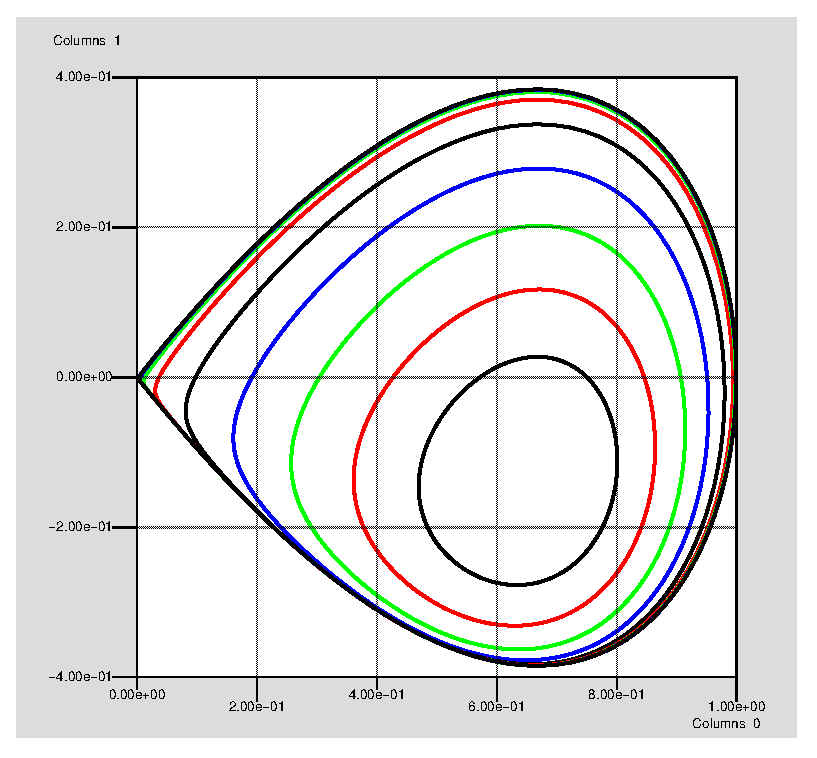
\includegraphics[scale=0.5]{include/hopfbif.eps}}
\put(200,0){
\put(157,148){(b)}
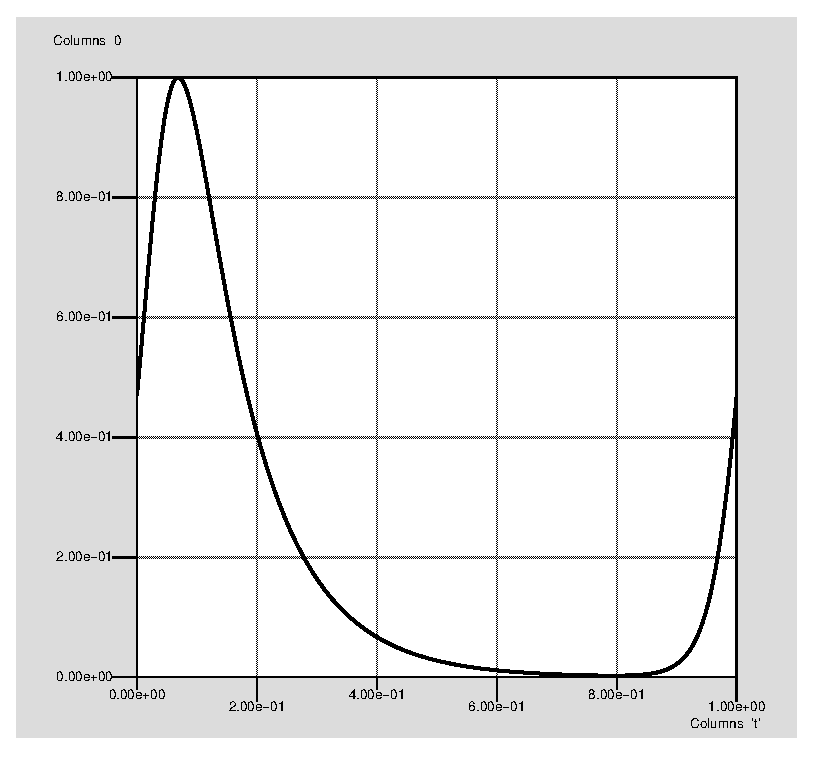
\includegraphics[scale=0.5]{include/notshifted.eps}}
\end{picture}
\caption{Periodic orbit growing from a Hopf bifurcation to a
  homoclinic orbit (a). The unshifted homoclinic orbit (b).}
\label{hopfbif}
\end{center}
\end{figure}

Note however, that the homoclinic orbit has the wrong left-hand and
right-hand end points. This can be seen by plotting the solution
corresponding to Label [13] using 't' vs. 'x' (coordinate [0]), 
as depicted in Figure~\ref{hopfbif}(b).

Hence, in order to continue this as a real homoclinic 
we have to give {\cal HomCont} special instructions, to do a phase-shift in
time. This can be done by setting \parf{ISTART=4}. Moreover, 
since we have not specified the value of
the equilibrium at the origin in \filef{ sib.c}, 
we need to set \parf{IEQUIB=1} to let
{\cal HomCont} detect the equilibrium. Note that in this case this is not
strictly necessary; however, we do this for instructional purposes.

Now we use {\cal HomCont} to continue the homoclinic orbit in $c$ and $\mu$ 
(\parf{PAR(3)}, \parf{PAR(5)}), to get the desired value $c=-2.0$.
\begin{center}
\commandf{ rn(c='sib.4',h='sib.shift',s='3') } \\
\commandf{ sv('4') }
\end{center}
\begin{verbatim}
  BR    PT  TY  LAB    PAR(3)        L2-NORM      ...    PAR(5)     
   3    51  EP   14  -2.00000E+00   4.01890E-01   ...  2.66146E-09
\end{verbatim}
The output is saved in the files \filef{ b.4}, \filef{ s.4} and
\filef{ d.4}. Note that \parf{PAR(5)}=$\mu$ remains zero, which is exactly
what we expect.

Next we want to add a solution to the adjoint equation to this
solution. This is achieved by making the change \parf{ ITWIST = 1}
saved in \filef{ h.sib.twist}. Also, we set \parf{ISTART} to 1 to tell 
{\cal HomCont} that it is should not try to shift the orbit anymore.
\begin{center}
\commandf{ rn(c='sib.5',h='sib.twist',s='4') } \\
\commandf{ sv('5') }
\end{center}
or, alternatively,
\begin{center}
\commandf{ cc("IRS",14) }\\
\commandf{ cc("ICP",[5,8])}\\
\commandf{ cc("NMX",2)}\\
\commandf{ hch("ITWIST",1)}\\
\commandf{ hch("ISTART",1)}\\
\commandf{ rn(s='4')}\\
\commandf{ sv('5')}
\end{center}
where \commandf{hch} means ``change {\cal HomCont} constant''.
The output is stored in \filef{ b.5}, \filef{ s.5}  and \filef{ d.5}.
\begin{verbatim}
  BR    PT  TY  LAB    PAR(5)        L2-NORM    ...    PAR(8)     
   3     2  EP   15   2.66146E-09   4.01890E-01 ...   1.00000E-02
\end{verbatim}
Here \parf{PAR(8)} is a dummy (unused) parameter and $\mu$ just stays where
it is. Now that we have obtained the solution of the adjoint equation,
we are able to detect inclination flips. This can be achieved by
setting \parf{NPSI} to 1, \parf{IPSI(1)} to 13, and monitoring \parf{PAR(33)}.
\begin{center}
\commandf{ rn(c='sib.6',h='sib.if',s='5') } \\
\commandf{ sv('6') }
\end{center} 
\begin{verbatim}
  BR    PT  TY  LAB    PAR(4)        L2-NORM    ...  PAR(5)        PAR(33)
   3    19  UZ   16   7.11774E-02   4.01890E-01 ... 1.24376E-11  -2.36702E-07
\end{verbatim}   
The output is stored in \filef{ b.6}, \filef{ s.6}  and \filef{ d.6}.
Hence an inclination flip was found at $\alpha=0.711774$.

Now we are ready to perform homoclinic branch switching, using
the techniques described in \cite{OlChKr:03}. 
Our first aim is to find a 2-homoclinic orbit. The
ingredients we need are: a homoclinic orbit where $n$-homoclinic orbits
are close by, and the solution to the adjoint equation to
obtain the Lin vector. Since both ingredients are there, we can now
continue in $\mu$, $\varepsilon_1$ and $T_1$, to obtain the initial
Lin gap. Recall from Chapter~\ref{ch:HomCont} that the Lin gaps 
$\varepsilon_i$ correspond to
\parf{PAR(20+i*2)} and the time intervals $T_i$ 
correspond to \parf{PAR(21+i*2)}. We stop when
$\varepsilon_1=0.2$. We need to specify \parf{ITWIST=2}, to tell 
{\cal HomCont} we
aim to find a 2-homoclinic orbit, so that it will split it up in three
parts with two potential Lin gaps. We effectively have a 9-dimensional
system at this point.
\begin{center}
\commandf{ rn(c='sib.7',h='sib.hbs2',s='6') } \\
\commandf{ sv('7') }
\end{center} 
\begin{verbatim}
  BR    PT  TY  LAB    PAR(21)       L2-NORM    ...  PAR(22)       PAR(5)     
   3    10       18   3.45897E+01   4.46818E-01 ... 7.87712E-07  -1.55885E-11
   3    20       19   2.73699E+01   4.46818E-01 ... 2.91119E-05  -1.63974E-09
   3    30       20   1.73720E+01   4.46817E-01 ... 4.42273E-03  -3.10167E-05
   3    38  EP   21   1.01451E+01   4.46796E-01 ... 2.00000E-01  -1.48615E-02
\end{verbatim}
The output is stored in \filef{ b.7}, \filef{ s.7}  and \filef{ d.7}.
Here we see that $T_1$, the time it takes to make the first loop with
respect to the Poincar\'e section, decreases. This is illustrated in
Figure~\ref{broken}. Next we are ready to close this gap, by continuing
in $\alpha$, $\mu$, and $\varepsilon_1$, while keeping $T_1$ at a
constant value.
\begin{figure}[htb]
\begin{center}
\begin{picture}(400,180)
\put(0,0){
\put(157,148){(a)}
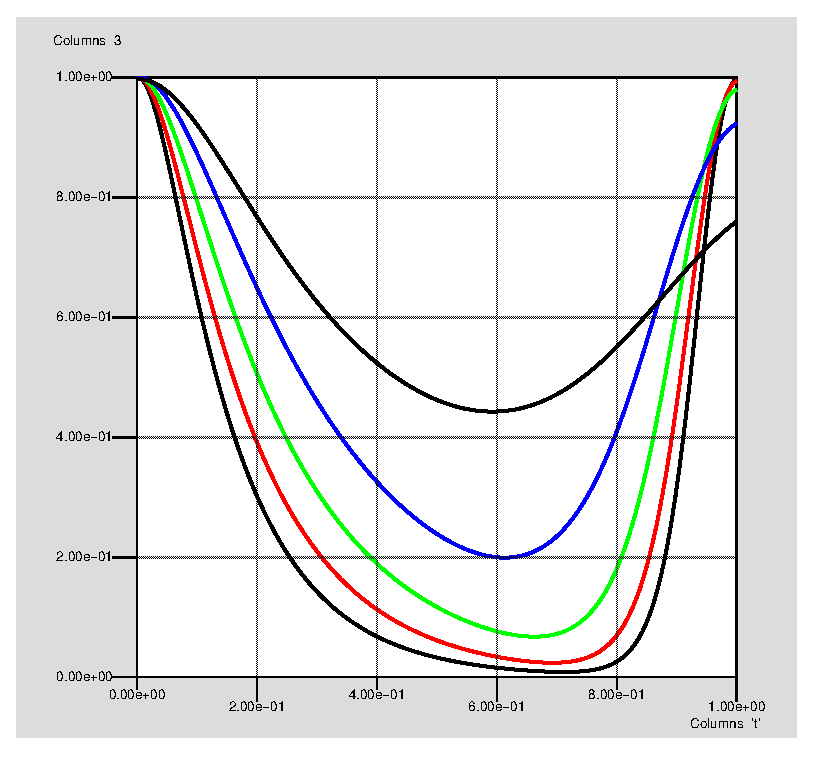
\includegraphics[scale=0.5]{include/loop.eps}}
\put(200,0){
\put(157,148){(b)}
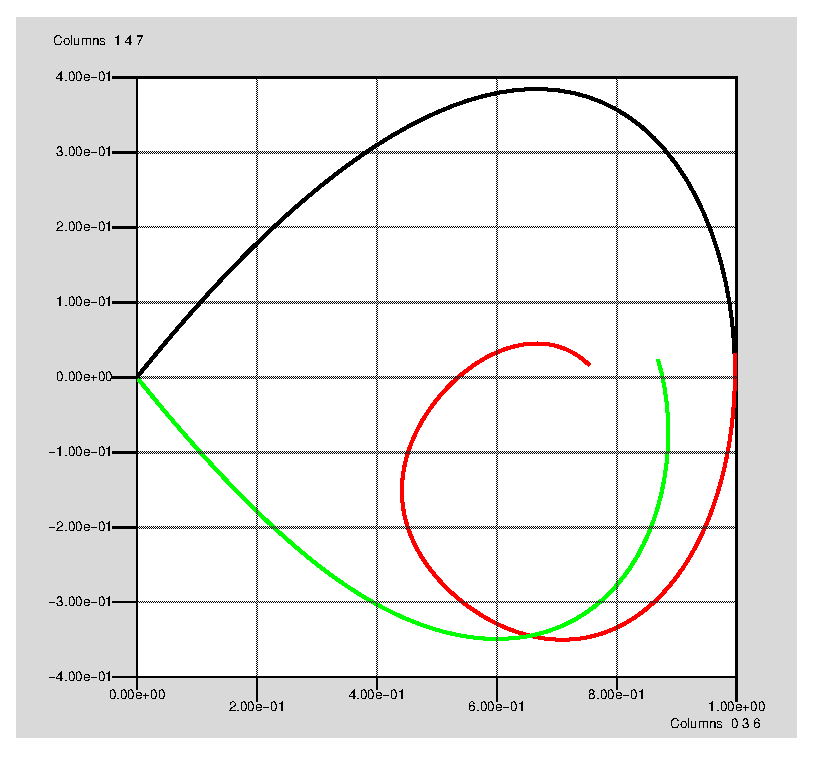
\includegraphics[scale=0.5]{include/broken.eps}}
\end{picture}
\caption{Behaviour of the second piece of the
`broken homoclinic orbit' when creating a Lin gap (a).
Projection of the ``broken homoclinic orbit''
onto the $(x,y)$-plane, where $\varepsilon_1=0.2$. To include all the
pieces necessary to obtain this
figure, the ``X'' box must contain [0,3,6] and the ``Y'' box must contain
[1,4,7] (b).}
\label{broken}
\end{center}
\end{figure}
\begin{center}
\commandf{ rn(c='sib.8',h='sib.hbs2',s='7') } \\
\commandf{ ap('6') }
\end{center} 
\begin{verbatim}
  BR    PT  TY  LAB    PAR(4)        L2-NORM    ...   PAR(5)        PAR(22)    
   3     3  UZ   22   7.40000E-02   4.46781E-01 ... -1.43162E-02   1.93746E-01
   3    32  EP   23   1.98414E-01   4.46590E-01 ... -6.05495E-03   2.29300E-06
\end{verbatim}
The output is appended to \filef{ b.6}, \filef{ s.6}  and \filef{  d.6}.
Now we have obtained a 2-homoclinic orbit at label 24. However, the
homoclinic orbit is still split in three parts. We can switch back to
a normal orbit by setting \parf{ITWIST} back to 0 and continuing in the usual
way. Here we continue back to the inclination flip point in $\alpha$
and $\mu$.
\begin{center}
\commandf{ rn(c='sib.9',h='sib.hom',s='6') } \\
\commandf{ ap('6') }
\end{center} 
\begin{verbatim}
  BR    PT  TY  LAB    PAR(4)        L2-NORM    ...   PAR(5)     
   3     7  UZ   24   1.50000E-01   4.94490E-01 ... -3.60248E-03
   3    30  EP   25   7.61403E-02   4.98746E-01 ... -2.64847E-06
\end{verbatim}
So the 2-homoclinic orbit converges back to the 1-homoclinic orbit at
the inclination flip bifurcation.
The output is appended to \filef{ b.6}, \filef{ s.6}  and \filef{  d.6}.
The resulting 2-homoclinic orbits can be seen using
\begin{center}
\commandf{ plot('6') }
\end{center} 
and is depicted in Figure~\ref{hom2.eps}(a).
\begin{figure}[htb]
\begin{center}
\begin{picture}(400,180)
\put(0,0){
\put(157,148){(a)}
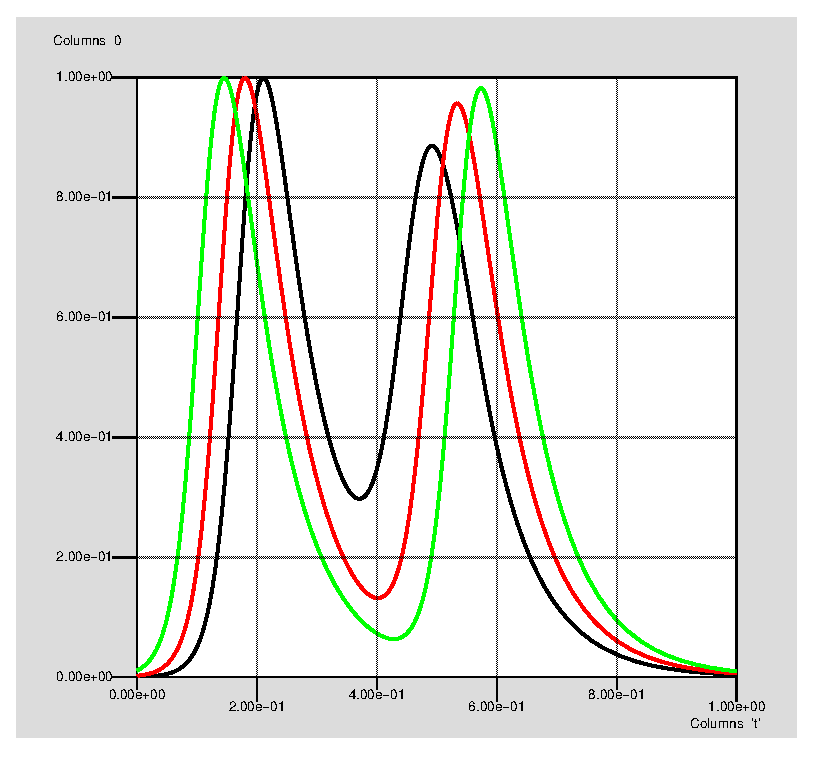
\includegraphics[scale=0.5]{include/hom2.eps}}
\put(200,0){
\put(157,148){(b)}
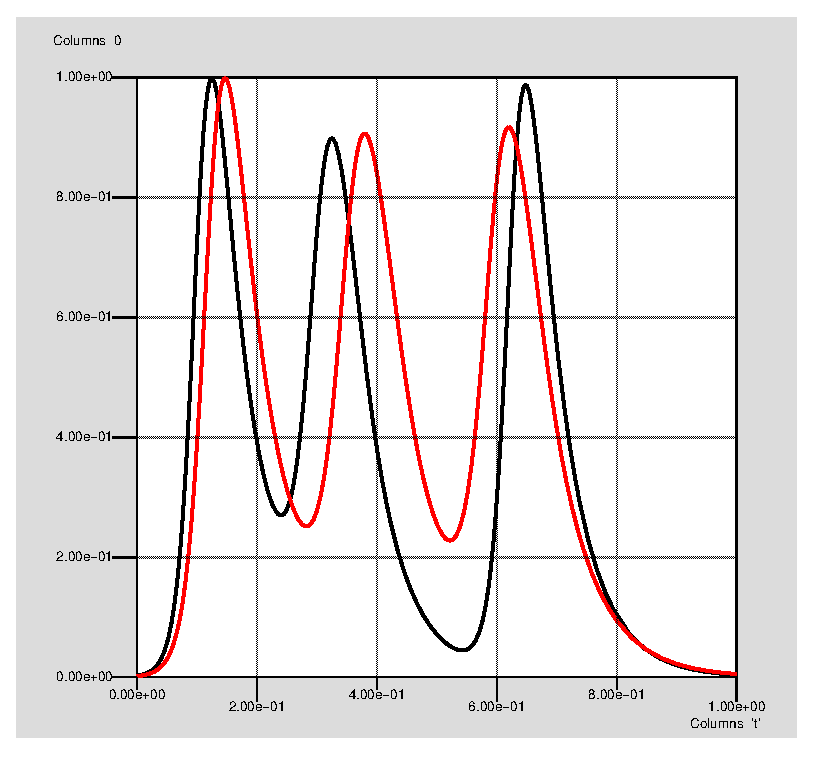
\includegraphics[scale=0.5]{include/hom3.eps}}
\end{picture}
\caption{The 2-homoclinic orbit as $a$ is changed (a).
The two different 3-homoclinic orbits (b).}
\label{hom2.eps}
\end{center}
\end{figure}

Next, we aim to find a 3-homoclinic orbit. To do so, we
restart at the inclination flip point at label 16 and set
\parf{ITWIST=3}. Moreover, we need to continue in one more
gap, $\varepsilon_2$=\parf{PAR(24)} and, once again, stop
when $\varepsilon_1$=\parf{PAR(22)=0}. Note that the 
dimension of the boundary value problem we continue
is now equal to 12. This is not to be confused with the setting
of \parf{NDIM=3} in the parameter file, because {\cal HomCont} handles this
internally.
\begin{center}
\commandf{ rn(c='sib.10',h='sib.hbs3',s='6') } \\
\commandf{ sv('10') }
\end{center} 
\begin{verbatim}
  BR    PT  TY  LAB    PAR(21)    ...   PAR(22)       PAR(24)       PAR(5)     
   3    10       26   3.45896E+01 ...  7.87894E-07   6.42157E-07  -1.06346E-11
   3    20       27   2.73699E+01 ...  2.91126E-05   6.51591E-07  -1.63655E-09
   3    30       28   1.73719E+01 ...  4.42289E-03   1.44090E-04  -3.10188E-05
   3    38  EP   29   1.01451E+01 ...  2.00000E-01   6.97445E-02  -1.48615E-02
\end{verbatim}
The output is stored in \filef{ b.10}, \filef{ s.10}  and \filef{ d.10}.
Now we need to subsequently close the Lin gaps. Our strategy is to
keep $T_1$ fixed. We first continue in $\alpha$, $\mu$,
$\varepsilon_1$ and $\varepsilon_2$ until $\varepsilon_1=0$.
\begin{center}
\commandf{ rn(c='sib.11',h='sib.hbs3',s='10') } \\
\commandf{ ap('6') }
\end{center} 
\begin{verbatim}
  BR    PT  TY  LAB    PAR(4)     ...   PAR(5)        PAR(22)       PAR(24)
   3     6  UZ   30   8.20000E-02 ... -1.29790E-02   1.76995E-01   6.37184E-02
   3    32  EP   31   1.98414E-01 ... -6.05495E-03   2.30717E-06   3.62449E-02
\end{verbatim}
The output is appended to \filef{ b.6}, \filef{ s.6}  and \filef{ d.6}.
Note that this continuation is very similar to the one where we found
a 2-homoclinic orbit. In fact we have now found a 2-homoclinic orbit
(numerically) followed by a `broken' 1-homoclinic orbit; only the mesh
is not aligned.

The next step is to close the gap corresponding to $\varepsilon_2$ to
obtain a 3-homoclinic orbit. We replace the continuation parameter
$\varepsilon_1$ by $T_2$, because $T_2$ (\parf{PAR(23)})
still has to be decreased from
its high value (35) and $\varepsilon_1$ needs to stay at 0.
\begin{center}
\commandf{ rn(c='sib.12',h='sib.hbs3',s='6') } \\
\commandf{ ap('6') }
\end{center} 
\begin{verbatim}
  BR    PT  TY  LAB    PAR(4)     ...   PAR(5)        PAR(23)       PAR(24)
   3    16  UZ   32   1.98395E-01 ... -6.05536E-03   2.01311E+01   1.82491E-08
   3    24  UZ   33   1.80000E-01 ... -6.50293E-03   1.27554E+01  -3.14294E-02
   3    30  UZ   34   1.66990E-01 ... -6.89269E-03   9.41745E+00  -1.03179E-06
   3    32  EP   35   1.78172E-01 ... -6.55364E-03   9.50300E+00  -7.20367E-02
\end{verbatim}
The output is appended to \filef{ b.6}, \filef{ s.6}  and \filef{ d.6}.
Note that we have found two zeros of \parf{PAR(24)}, at labels 32 and
34, respectively. The two zeros
correspond to two different 3-homoclinic
orbits, which, when followed from periodic orbits, both emanate from
from the same saddle-node bifurcation.
These two 3-homoclinic orbits are depicted in Figure~\ref{hom2.eps}(b).
We can follow both of these back to the inclination flip point, by
setting \parf{ITWIST} back to 0:
\begin{center}
\commandf{ rn(c='sib.13',h='sib.hom',s='6') } \\
\commandf{ ap('6') }
\end{center} 
\begin{verbatim}
  BR    PT  TY  LAB    PAR(4)        L2-NORM    ...   PAR(5)     
   3    13  UZ   36   1.29999E-01   5.04807E-01 ... -2.33902E-03
   3    30  EP   37   9.27258E-02   5.06560E-01 ... -2.76788E-04
\end{verbatim}
\begin{center}
\commandf{ rn(c='sib.14',h='sib.hom',s='6') } \\
\commandf{ ap('6') }
\end{center}
\begin{verbatim}
  BR    PT  TY  LAB    PAR(4)        L2-NORM    ...   PAR(5)     
   3     7  UZ   38   1.45000E-01   5.47347E-01 ... -4.79400E-03
   3    30  EP   39   8.39401E-02   5.52605E-01 ... -7.36741E-05
\end{verbatim}
All the output is appended to \filef{ b.6}, \filef{ s.6}  and \filef{  d.6}.
The bifurcation diagram and the paths we followed when closing the Lin
gaps are depicted in Figure~\ref{parspace}. It is possible and
straightforward to obtain $4, 5, 6, \dots$-homoclinic orbits by 
extending the above strategy.
\begin{figure}[htb]
\begin{center}
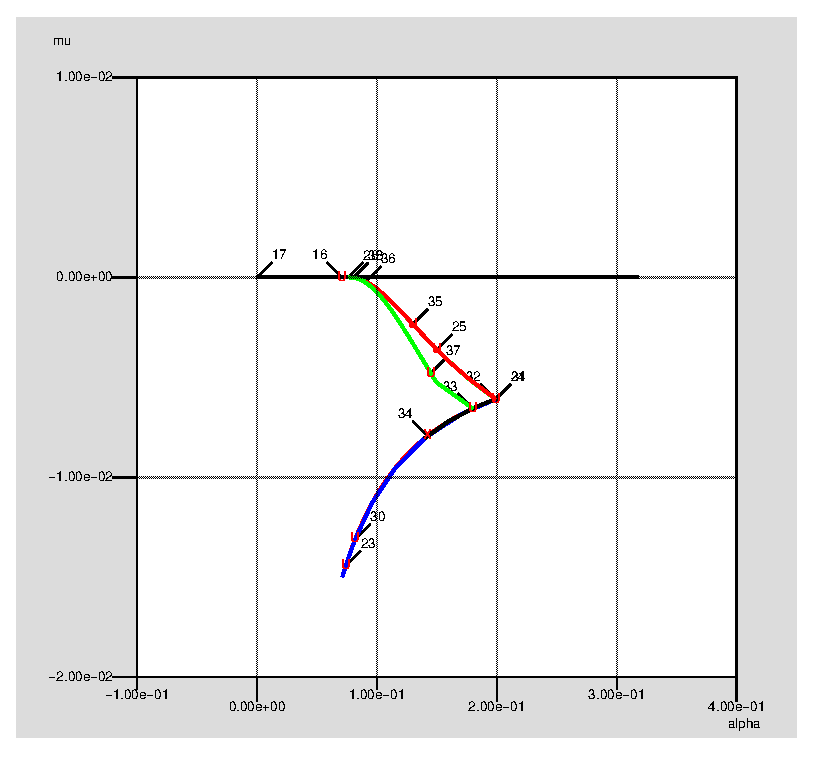
\includegraphics[scale=0.5]{include/parspace.eps}
\caption{Parameter space diagram near an inclination flip. 
The curve
through label 17 corresponds to a 1-homoclinic orbit. 
The opening of the Lin gaps occurs along the vertical line from
label 16 to label 23. The curves
through labels 23 and 30 denote the path that is followed when
closing the Lin gaps. The (approximately overlaid)
curves though labels 25 and 35 correspond to the 
2- and one of the 3-homoclinic orbits.
Finally, the curve through label 37 corresponds to the other
3-homoclinic orbit, which was obtained for \parf{PAR(22)}=$T_2=12.03201$.}
\label{parspace}
\end{center}
\end{figure}

\section{ Branch switching for a Shil'nikov type homoclinic orbit in
the FitzHugh-Nagumo equations.}

The FitzHugh-Nagumo (FHN) equations \cite{FitzH:61,NaArYo:62} 
are a simplified version of the
Hodgkin-Huxley equations \cite{HoHu:52}. 
They model nerve axon dynamics and are given by

\begin{equation}
\begin{split}
u_t&=u_{xx}-f_a(u)-w, \\
w_t&=\epsilon(u-\gamma w),
\end{split}
\label{fhnpde}
\end{equation}
where
\[
f_a(u) = u (u-a)(u-1).
\]

Travelling wave solutions of the form $(u,w)(x,t)=(u,w)(\xi)$, where
$\xi=x+ct$ are solutions of the following ODE system:

\begin{equation}
\begin{split}
\dot u &= v,\\
\dot v &= c v + f_a(u) + w,\\
\dot w &= \frac{\epsilon}{c} (u - \gamma w).
\end{split}
\label{fhnode}
\end{equation}
In particular we consider solitary wave solutions of \eqref{fhnpde}.
These correspond to orbits homoclinic to $(u,v,w)=0$ in system \eqref{fhnode}.
In our numerical example we keep $\gamma=0$.

We aim to find a $2$-homoclinic orbit at a Shil'nikov bifurcation.
All the commands given here are in the file fnb.auto.
First we obtain a homoclinic orbit using a homotopy technique (see
\citeasnoun{FrDoMo:94}), using \parf{ISTART=3}, for the parameter 
values $c=0.21, a=0.2, \epsilon=0.0025$.

\begin{center}
\commandf{ demo('sib') }\\
\commandf{ld('fnb')}\\
\commandf{rn()}\\
\commandf{sv('1')}
\end{center}

Among the output we see:
\begin{verbatim}
  BR    PT  TY  LAB     PERIOD       L2-NORM    ...   PAR(17)
   1    20  UZ    3   2.92257E+01   2.37916E-01 ... -1.68000E-09
\end{verbatim}
and a zero of \parf{PAR(17)} means that a zero of an artificial parameter has
been located and the right-hand end point of the corresponding
solution belongs to the plane that is tangent to the stable manifold
at the saddle. This point still needs to come closer to the
equilibrium, which we can achieve by further increasing the period to
300, while keeping \parf{PAR(17)} at 0:
\begin{center}
\commandf{rn(c='fnb.2',h='fnb.1',s='1')}\\
\commandf{sv('2')}
\end{center}
\begin{verbatim}
  BR    PT  TY  LAB     PERIOD       L2-NORM    ...   PAR(2)
   1   190  UZ   10   3.00000E+02   7.37932E-02 ...  1.79286E-01
\end{verbatim}

Next we stop using the homotopy technique and increase the period even
further, to 1000.
\begin{center}
\commandf{rn(c='fnb.3',h='fnb.3',s='2')}\\
\commandf{sv('3')}
\end{center}
\begin{verbatim}
  BR    PT  TY  LAB     PERIOD       L2-NORM    ...   PAR(2)
   1    80  UZ   13   1.00000E+03   4.04183E-02 ...  1.79286E-01
\end{verbatim}

A continuation in \parf{PAR(2)}=$a$ and \parf{PAR(1)}=$c$ needs to be 
performed to arrive
at the place where we wish to find a 2-homoclinic orbit: $a=0$. At the
same time we monitor \parf{PAR(22)} to locate Belyakov points.
\begin{center}
\commandf{rn(c='fnb.4',h='fnb.4',s='3')}\\
\commandf{sv('4')}
\end{center}
\begin{verbatim}
  BR    PT  TY  LAB    PAR(2)        L2-NORM    ...   PAR(1)        PAR(22)
   1     6  UZ   15   1.31812E-01   3.28710E-02 ...  2.17166E-01  -6.31243E-06
   1    23  UZ   19  -8.54548E-08   1.56158E-02 ...  2.74218E-01  -9.88772E-02
\end{verbatim}
Hence, there exists a Belyakov point at $(a,c)=(0.131812,0.21766)$.
At label 19 we have a lower value of $a$ than at the Belyakov point,
and by inspection of the file
\filef{d.4} we can observe that the equilibrium has one positive
eigenvalue and a complex conjugate pair of eigenvalues with negative
real part, and conclude that this orbit is of Shil'nikov type.
Before starting the homoclinic branch switching, we calculate
the adjoint to obtain a `Lin vector':
\begin{center}
\commandf{rn(c='fnb.5',h='fnb.5',s='4')}\\
\commandf{sv('5')}
\end{center}
\begin{verbatim}
  BR    PT  TY  LAB    PAR(9)        L2-NORM    ...   PAR(3)     
   1     2  EP   28  -1.00000E+00   1.56158E-02 ...  2.50000E-03
\end{verbatim}
Next, we continue in the time $T_1$ (\parf{PAR(21)}), the gap
$\varepsilon_1$ (\parf{PAR(22)}) and $c$ (\parf{PAR(1)}), 
and by setting \parf{ISTART}=-2
we try to locate a 2-homoclinic orbit:
\begin{center}
\commandf{rn(c='fnb.6',h='fnb.6',s='5')}\\
\commandf{sv('6')}
\end{center}
In fact we find many of them, exactly as is predicted by the theory:
\begin{verbatim}
  BR    PT  TY  LAB    PAR(21)    ...   PAR(1)        PAR(22)
... 
   1   175  UZ   46   1.64818E+02 ...  2.74218E-01   4.59218E-16
   1   180  UZ   47   1.44759E+02 ...  2.74218E-01  -1.43728E-14
   1   184  UZ   48   1.24939E+02 ...  2.74218E-01   1.55506E-13
   1   189  UZ   49   1.04615E+02 ...  2.74218E-01  -2.37665E-11
   1   193  UZ   50   8.53538E+01 ...  2.74218E-01   1.02165E-11
   1   198  UZ   51   6.37899E+01 ...  2.74218E-01  -5.74204E-14
\end{verbatim}
Each of these homoclinic orbits differ 
by about 20 in the value $T_1$. This is about 
the time it takes to make one half-turn close to and
around the equilibrium, so that orbits differ by the number of 
half turns around the equilibrium before a big excursion
in phase space. Note that the variation of 
$c$ is so small that it does not appear.

A plot of $T_1$ vs. $\varepsilon_1$ gives insight into how the gap
is opened and closed in the continuation process. This is depicted in 
Figure~\ref{shilgap}.
\begin{figure}[htb]
\begin{center}
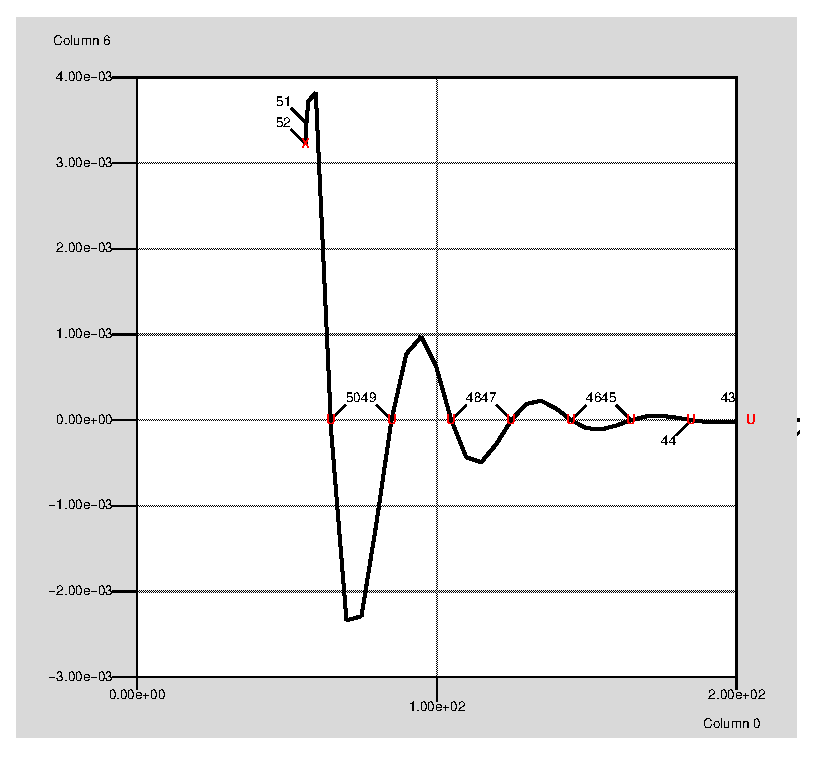
\includegraphics[scale=0.5]{include/shilgap.eps}
\caption{A plot of $\varepsilon_1$ as a function of $T_1$ 
during our computation of Shil'nikov-type two-homoclinic orbits. 
Each zero corresponds to a different orbit.}
\label{shilgap}
\end{center}
\end{figure}
We are now in a
position to continue each of these orbits as a
normal homoclinic orbit by setting \parf{ISTART=1} and
\parf{ITWIST=0}. We leave
this as an exercise to the reader.

\section{ Branch switching to a 3-homoclinic orbit in
a\\ 5th-order Korteweg-De Vries model}

In \citeasnoun{ChGr:97} the following water wave model was considered:
\begin{equation}
\frac{2}{15}r''''-b r''+ar+\frac{3}{2}r^2-
\frac{1}{2}(r')^2+[rr']' = 0.
\label{cgode}
\end{equation}
It represents solitary-wave solutions $r(x+at)$, $r\to 0$ as $x\to
\pm\infty$ of the 5th-order PDE
\[
r_t+\frac{2}{15}r_{xxxx}-b r_{xxx}+3r r_x+2 r_x r_{xx}+r r_{xxx=0},
\]
where $a$ is the wave speed.
The ODE corresponds to a Hamiltonian system with Hamiltonian
\[ H=-\frac{1}{2}q_1^3-\frac{1}{2}a q_1^2+p_1 q_2-\frac{1}{2}b q_2^2+
\frac{15}{4}p_2^2+\frac{1}{2}q_2^2 q_1 \]
and 
\[q_1=r, \quad q_2=r', \quad p_1=-\frac{2}{15}r'''+br'-rr', \quad p_2=\frac{2}{15}r''.\]
System \eqref{cgode} is also reversible under the transformation 
\[ t \mapsto -t, (q_1,q_2,p_1,p_2)\mapsto (q_1,-q_2,-p_1,p_2),\] 
but we do not exploit the reversible structure (\parf{IREV=0}), and
instead use it as an example of Hamiltonian system.
This system exhibits an orbit flip for a reversible Hamiltonian system.
In Hamiltonian systems, homoclinic orbits are codimension-zero
phenomena, and we have to add an additional parameter $\lambda$ that breaks
the Hamiltonian structure in this system, by introducing artificial friction.
Thus, the actual system of equations that is
used for continuation is
\[\dot x=(\lambda I + J)\nabla H(x),\]
where $x=(q_1,q_2,p_1,p_2)$ and $J$ is the usual skew symmetric matrix
in $\mathbb{R}^4$.
It is now possible to continue a homoclinic orbit in {\cal HomCont} in two
parameters ($\lambda$ and either $a$ or $b$); see also
\citeasnoun{Be:90a}.

An explicit solution exists for $a=3/5(2b+1)(b-2), b\geq -1/2$, and it is
given by 
\[r(t)=3(b+\frac{1}{2})\mathrm{sech}^2\left([\frac{3}{4}(2b+1)]^{1/2}t\right).\]
It corresponds to a reversible orbit flip for $b>2$ ($a>0$) 
We start from this explicit solution, using \parf{ISTART=2}, for $a=3$ and
$b=(\sqrt{65}+3)/4$:

\begin{center}
\commandf{demo('kdv') }\\
\commandf{ld('kdv')}\\
\commandf{rn()}\\
\commandf{sv('1')}
\end{center}
\begin{verbatim}
  BR    PT  TY  LAB    PAR(1)        L2-NORM    ...   PAR(3)     
   1     1  EP    1   3.00000E+00   5.56544E+00 ...  0.00000E+00
   1     2  EP    2   3.04959E+00   5.49141E+00 ...  1.77919E-17
\end{verbatim}
Here \parf{PAR(1)}=$a$, \parf{PAR(2)}=$b$, and
\parf{PAR(3)}=$\lambda$. We have only done a
very small continuation to give \AUTO a chance to create a good mesh
and avoid convergence problems later.
Next, we set \parf{ITWIST=1} and calculate the adjoint:
\begin{center}
\commandf{rn(c='kdv.2',h='kdv.2',s='1')}\\
\commandf{sv('2')}
\end{center}
\begin{verbatim}
  BR    PT  TY  LAB    PAR(2)        L2-NORM    ...   PAR(9)
   1     2  EP    3   2.76556E+00   5.49140E+00 ... -7.62944E-08
\end{verbatim}
We now need to move back to the orbit flip at $a=3$:
\begin{center}
\commandf{rn(c='kdv.3',h='kdv.3',s='2')}\\
\commandf{sv('3')}
\end{center}
\begin{verbatim}
  BR    PT  TY  LAB    PAR(1)        L2-NORM    ...   PAR(3)     
   1    14  UZ    5   3.00000E+00   5.47612E+00 ...  1.47274E-09
\end{verbatim}
Now all preparations are done to start homoclinic branch
switching. This is very similar to the technique used in 
Sandstede's model in Section~\ref{sec:HomCont_hbs_san}; 
to find a 3-homoclinic orbit, we open 2 Lin gaps,
until $T_1=3.5$, while also varying $\lambda$=\parf{PAR(3)}.
\begin{center}
\commandf{rn(c='kdv.4',h='kdv.4',s='3')}\\
\commandf{sv('4')}
\end{center}
\begin{verbatim}
  BR    PT  TY  LAB    PAR(3)     ...   PAR(21)       PAR(22)       PAR(24)
   1    13        8   6.31458E-10 ...  1.65469E+01  -8.57681E-08  -7.30773E-07
   1    23  UZ    9   1.46493E-09 ...  9.92489E+00  -5.84373E-12   1.93098E-07
   1    26       10   4.01320E-09 ...  6.92406E+00   2.59555E-07   7.47534E-07
   1    33  EP   11   2.15487E-06 ...  3.50000E+00   7.92587E-04   3.98390E-04
\end{verbatim}
We then look for an orbit with $a<3$ and close the gap corresponding 
to $\varepsilon_1$=\parf{PAR(22)}, for decreasing $a$.
\begin{center}
\commandf{rn(c='kdv.5',h='kdv.5',s='4')}\\
\commandf{sv('5')}
\end{center}
\begin{verbatim}
  BR    PT  TY  LAB    PAR(2)     ...   PAR(3)        PAR(22)       PAR(24)
   1    10       12   2.58030E+00 ...  2.15869E-06   7.65037E-04   3.82464E-04
   1    13  UZ   13   2.32044E+00 ...  4.02730E-11   1.17522E-10   1.69655E-08
   1    20  EP   14  -1.14985E-01 ... -8.87194E-04  -7.18231E-01  -3.31153E-01
\end{verbatim}
and finally close the gap corresponding to $\varepsilon_2$=\parf{PAR(24)},
\begin{center}
\commandf{rn(c='kdv.6',h='kdv.6',s='5')}\\
\commandf{sv('6')}
\end{center}
\begin{verbatim}
  BR    PT  TY  LAB    PAR(2)     ...   PAR(3)        PAR(23)       PAR(24)
   1    35       15   2.31893E+00 ... -2.16070E-08   7.69046E+00  -1.08126E-05
   1    51  UZ   16   2.34039E+00 ...  2.83533E-07   3.47976E+00   1.42651E-04
   1    58  UZ   17   3.08085E+00 ...  1.84952E-12   3.50004E+00  -1.64827E-10
   1    70  EP   18   3.08870E+00 ... -8.10422E-08   5.87541E+00  -4.82991E-05
\end{verbatim}
so that a three-homoclinic orbit is found. Here the zero at label
16 is the one we are looking for. At label 17, $a$=\parf{PAR(1)} 
has changed
considerably to the extend that $a>3$ and a second 3-homoclinic orbit 
is found. Note that for all zeros of \parf{PAR(24)}=$\varepsilon_2$, the
parameter $\lambda$=\parf{PAR(3)} is also zero (within \AUTO accuracy), 
which it has to be to remain
within the original Hamiltonian system.
Setting \parf{ISTART=1}, a normal ``trivial'' continuation (with \parf{NMX=1})
of the orbit corresponding to label 16
lets {\cal HomCont} produce a proper concatenated
3-homoclinic orbit:
\begin{center}
\commandf{rn(c='kdv.7',h='kdv.7',s='6')}\\
\commandf{sv('7')}
\end{center}
\begin{verbatim}
  BR    PT  TY  LAB    PAR(2)        L2-NORM    ...   PAR(3)     
   1     1  EP   19   2.34039E+00   7.51157E+00 ...  2.83533E-07
\end{verbatim}
This 3-homoclinic orbit is depicted in Figure~\ref{kdv3hom}.
\begin{figure}[htb]
\begin{center}
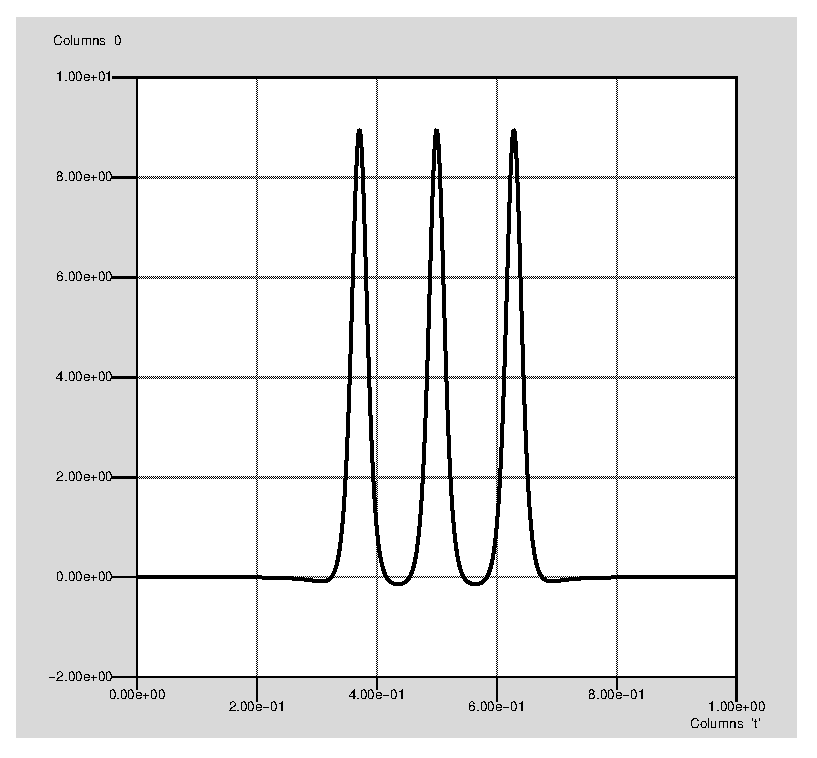
\includegraphics[scale=0.5]{include/kdv3hom.eps}
\caption{A 3-homoclinic orbit in a 5th-order Hamiltonian 
Korteweg-De Vries model.}
\label{kdv3hom}
\end{center}
\end{figure}

%==============================================================================
%==============================================================================


\bibliography{include/auto} \label{sec:bibliography}


\end{document}
